% document class -------------------------------------------
\documentclass[11pt,oneside,openright]{./style/phdthesis}
% ----------------------------------------------------------

% my definitions -------------------------------------------
%\def\qpsk{}
%\def\optical{}
\def\bpsk{}
%\def\mQAM{}
%\def\sdf{}
%\def\dsp{}
\def\quantumRNG{}
%\def\bb{}
%\def\qokd{}
%\def\quantumA{}
%\def\cvQuantum{}
%\def\intradyne{}
\def\classicalMpc{}
\def\quantumMpc{}

% ----------------------------------------------------------

% my packages ----------------------------------------------
\usepackage{amsmath}
\usepackage[ansinew]{inputenc}
%\usepackage[portuguese]{babel}
\usepackage[printonlyused, withpage]{acronym}
\usepackage{a4wide}
\usepackage{palatino}
\usepackage{fancyhdr}
\usepackage{fancybox}
\usepackage{amssymb}

% biblatex ------------------------------------------------------------------------------------------
% used to divide the bibliography into multiple parts for example per chapter or per section
\usepackage[sorting=none, backend=biber]{biblatex}
% ---------------------------------------------------------------------------------------------------

%\usepackage{chapterbib} %com este package as referencias bibliográficas aparecem no final de cada capítulo
%\usepackage{cite}
\usepackage{epsfig}
%\usepackage{subfigure}
\usepackage{graphics}
\usepackage{float}
\usepackage{here}
\usepackage[T1]{fontenc}
\usepackage{rotating}
\usepackage{multirow}
%\usepackage{comment}
%\usepackage{captionhack}
\usepackage{epigraph}
\usepackage[linkcolor=black]{hyperref}
%\renewcommand{\thesubfigure}{}
\hypersetup{colorlinks=true}
\usepackage{enumerate}
%\usepackage[numbers,sort&compress]{natbib}
%\usepackage{hypernat}
\usepackage{booktabs}
\usepackage{url}                    % needed to cite a site
\usepackage{eurosym}
\usepackage{makeidx}
\usepackage{datatool}
\usepackage[toc, acronym]{glossaries}
\usepackage{graphicx}
\usepackage{caption}
\usepackage{subcaption}

\usepackage{tabulary}
\usepackage{braket}

% subfile handling packages
\usepackage{subfiles}

% For box
\usepackage{multicol}
\usepackage{tcolorbox}
\usepackage{booktabs}

% For flow chart
\usepackage{tikz}
\usetikzlibrary{shapes,arrows}

\usepackage{epstopdf}
\usepackage{listings}
\usepackage{color}
\usepackage{textcomp,xcolor}

\usepackage{mathrsfs}



% ----------------------------------------------------------

% my bib files ---------------------------------------------
%%%%%%%%%%%%%%%%%%%%%%%%%%%%%%%%%%%%%%%%%%%%%%%%%%%%%%%%%%%%%%%%%%%%%%%%%%%%%%%%%%
% Bibliography for the Simulator Strucuture
%%%%%%%%%%%%%%%%%%%%%%%%%%%%%%%%%%%%%%%%%%%%%%%%%%%%%%%%%%%%%%%%%%%%%%%%%%%%%%%%%%

\addbibresource{./chapter/simulator_structure/simulator_structure.bib}

%%%%%%%%%%%%%%%%%%%%%%%%%%%%%%%%%%%%%%%%%%%%%%%%%%%%%%%%%%%%%%%%%%%%%%%%%%%%%%%%%%
% Bibliography for SDF
%%%%%%%%%%%%%%%%%%%%%%%%%%%%%%%%%%%%%%%%%%%%%%%%%%%%%%%%%%%%%%%%%%%%%%%%%%%%%%%%%%

\ifdefined\qpsk         \addbibresource{./sdf/qpsk_transmitter/qpsk_transmitter.bib}\fi
\ifdefined\optical      \addbibresource{./sdf/optical_detection/optical_detection.bib}\fi
\ifdefined\bpsk         \addbibresource{./sdf/bpsk_system/bpsk_system.bib}\fi
\ifdefined\mQAM         \addbibresource{./sdf/m_qam_system/m_qam_system.bib}\fi
\ifdefined\simplified   \addbibresource{./sdf/simplified_coherent_receiver/simplified_coherent_receiver.bib}\fi
\ifdefined\dsp          \addbibresource{./sdf/dsp_laser_phase_compensation/dsp_laser_phase_compensation.bib}\fi
\ifdefined\quantumRNG   \addbibresource{./sdf/quantum_random_number_generator/quantum_random_number_generator.bib}\fi
\ifdefined\bb           \addbibresource{./sdf/bb84_with_discrete_variables/bb84_with_discrete_variables.bib}\fi
\ifdefined\qokd         \addbibresource{./sdf/qokd_with_discrete_variables/qokd_with_discrete_variables.bib}\fi
\ifdefined\quantumA     \addbibresource{./sdf/quantum_noise/quantum_noise.bib}\fi
\ifdefined\cvQuantum    \addbibresource{./sdf/cv_system/cv_system.bib}\fi
\ifdefined\intradyne    \addbibresource{./sdf/intradyne_cv_system/intradyne_cv_system.bib}\fi
\ifdefined\classicalMpc \addbibresource{./sdf/classical_mpc/classical_mpc.bib}\fi
\ifdefined\classicalMpc \addbibresource{./sdf/quantum_mpc/quantum_mpc.bib}\fi

%%%%%%%%%%%%%%%%%%%%%%%%%%%%%%%%%%%%%%%%%%%%%%%%%%%%%%%%%%%%%%%%%%%%%%%%%%%%%%%%%%
% Bibliography for the Library
%%%%%%%%%%%%%%%%%%%%%%%%%%%%%%%%%%%%%%%%%%%%%%%%%%%%%%%%%%%%%%%%%%%%%%%%%%%%%%%%%%

\addbibresource{./lib/snr_photoelectron_generator/snr_photoelectron_generator.bib}

%%%%%%%%%%%%%%%%%%%%%%%%%%%%%%%%%%%%%%%%%%%%%%%%%%%%%%%%%%%%%%%%%%%%%%%%%%%%%%%%%%
% Bibliography for the Algorithms
%%%%%%%%%%%%%%%%%%%%%%%%%%%%%%%%%%%%%%%%%%%%%%%%%%%%%%%%%%%%%%%%%%%%%%%%%%%%%%%%%%

\addbibresource{./algorithms/fft/fft.bib}

% ----------------------------------------------------------

% my commands ----------------------------------------------
\newcommand{\onlyinsubfile}[1]{#1}
\newcommand{\notinsubfile}[1]{}
\renewcommand{\textfraction}{0.01}
\renewcommand{\topfraction}{0.99}
\renewcommand{\floatpagefraction}{0.99}
\renewcommand{\bottomfraction}{0.99}
\renewcommand{\heavyrulewidth}{1pt}
\renewcommand{\lightrulewidth}{0.50pt}
\renewcommand{\chaptername}{Chapter}
\renewcommand{\figurename}{Figure}
\renewcommand{\appendixname}{\Large{Anex}}
\renewcommand{\tablename}{Table}
\renewcommand{\acronymname}{Acronimous}

\newcommand{\mli}[1]{\mathit{#1}}
\newcommand{\intSpace}{\!\!\!\!}
\newcommand{\doubleInt}{\!\!\int\intSpace\int\!\!}
\newcommand{\TX}{\mathit{TX}}
\newcommand{\NLI}{\mathit{NLI}}
\newcommand{\eff}{\mathit{eff}}
\newcommand{\LOASE}{\mathit{LO-ASE}}
\newcommand{\LONLI}{\mathit{LO-NLI}}


%\makesavenoteenv{tabular}



\hyphenpenalty=50000
\tolerance=10000
%%% General page formatting

\oddsidemargin 0.2in
\evensidemargin 0in
%\textwidth 155mm
\headheight 15.0pt
\topmargin 0in
%\textheight 237mm

% footheight 1.0in

\makeatletter
\providecommand*{\diff}%
{\@ifnextchar^{\DIfF}{\DIfF^{}}}
\def\DIfF^#1{%
\mathop{\mathrm{\mathstrut d}}%
\nolimits^{#1}\gobblespace}
\def\gobblespace{%
\futurelet\diffarg\opspace}
\def\opspace{%
\let\DiffSpace\!%
\ifx\diffarg(%
\let\DiffSpace\relax
\else
\ifx\diffarg[%
\let\DiffSpace\relax
\else
\ifx\diffarg\{%
\let\DiffSpace\relax
\fi\fi\fi\DiffSpace}

\providecommand*{\tDeriv}[3][]{%
\frac{\diff^{#1}#2}{\diff #3^{#1}}}
\providecommand*{\pDeriv}[3][]{%
\frac{\partial^{#1}#2}%
{\partial #3^{#1}}}

\graphicspath{{./figures/}{./sdf/bpsk_system/figures/}{./sdf/cv_system/figures/}}


\DeclareMathOperator{\erf}{erf}
\DeclareMathOperator{\erfc}{erfc}
\DeclareMathOperator{\sinc}{sinc}
\DeclareMathOperator{\R}{Re}
\DeclareMathOperator{\I}{Im}
\DeclareMathOperator{\asinh}{asinh}

%\newcommand{\publ}{}

\pagenumbering{arabic} 
% ----------------------------------------------------------

% index ----------------------------------------------------
\makeindex
% ----------------------------------------------------------


\begin{document}

% title -----------------------------------------------------
\title{NetXPTO - LinkPlanner}
\author{Armando Nolasco Pinto}
\date{\today}
\maketitle
% -----------------------------------------------------------

% table of contents -----------------------------------------
\tableofcontents
% -----------------------------------------------------------

% chapters --------------------------------------------------
%
% ------------------------------------------------------------------------
\chapter{Preface}

Th



%\include{chapter/introduction}
%
% ------------------------------------------------------------------------
\chapter{Simulator Structure}

\begin{refsection}



LinkPlanner is a signals open-source simulator.

The major entity is the system.

A system comprises a set of blocks.

The blocks interact with each other through signals.

\section{System}

\section{Blocks}

\section{Signals}

List of available signals:

\begin{itemize}
    \item Signal

\end{itemize}

\subsubsection{PhotonStreamXY}
A single photon is described by two amplitudes $A_x$ and $A_y$ and a phase difference between them, $\delta$. This way, the signal PhotonStreamXY is a structure with two complex numbers, $x$ and $y$.


\subsubsection{PhotonStreamXY\_MP}
The multi-path signals are used to simulate the propagation of a quantum signal when the signal can follow multiple paths. The signal has information about all possible paths, and a measurement performed in one path immediately affects all other possible paths.
From a Quantum approach, when a single photon with a certain polarization angle reaches a $50:50$ Polarizer, it has a certain probability of follow one path or another. In order to simulate this, we have to use a signal PhotonStreamXY\_MP, which contains information about all the paths available. In this case, we have two possible paths: $0$ related with horizontal and $1$ related with vertical. This signal is the same in both outputs of the polarizer. The first decision is made by the detector placed on horizontal axis. Depending on that decision, the information about the other path $1$ is changed according to the result of the path $0$. This way, we guarantee the randomness of the process. So, signal PhotonStreamXY\_MP is a structure of two PhotonStreamXY indexed by its path.


\section{Log File}
\subsection{Introduction}
The Log File allows for a detailed analysis of a simulation. It will output a file containing the timestamp when a block is initialized, the number of samples in the buffer ready to be processed for each input signal, the signal buffer space for each output signal and the amount of time in seconds that took to run each block. Log File is enabled by default, so no change is required. If you want to turn it off, you must call the set method for the logValue and pass $false$ as argument. This must be done before method $run()$ is called, as shown in line 125 of Figure \ref{fig:logfileexample}.

\renewcommand{\figurename}{Figure}
\begin{figure}[H]
\centering
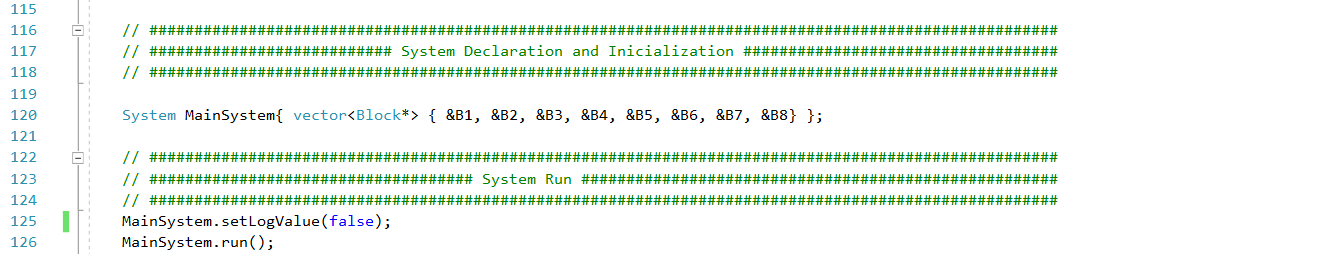
\includegraphics[width=1.3\linewidth]{./chapter/simulator_structure/figures/log_file_example}
\caption{Disabling Log File}
\label{fig:logfileexample}
\end{figure}

\subsection{Parameters}
The Log File accepts two parameters: $logFileName$ which correspond to the name of the output file, i.e., the file that will contain all the information listed above and $logValue$ which will enable the Log File if $true$ and will disable it if $false$.
\begin{table}[H]
\centering
\begin{tabulary}{1.0\textwidth}{|p{6cm}|p{4cm}|p{5cm}|}
\hline
\multicolumn{3}{|c|}{ \textbf{Log File Parameters} } \\
\hline
\textbf{Parameter}     & \textbf{Type}       & \textbf{Default Value} \\ \hline
logFileName            & string	             & "log.txt"\\ \hline
logValue               & bool	             & true\\ \hline
\end{tabulary}
\end{table}

\begin{table}[H]
\centering
\begin{tabulary}{1.0\textwidth}{|p{6cm}|p{4cm}|p{5cm}|}
\hline
\multicolumn{3}{|c|}{ \textbf{Available Set Methods} } \\
\hline
\textbf{Parameter}                    & \textbf{Type}        & \textbf{Comments} \\ \hline
setLogFileName(string newName)        & void	             & Sets the name of the output file to the name given as argument\\ \hline
setLogValue(bool value)               & void	             & Sets the value of logValue to the value given as argument\\ \hline
\end{tabulary}
\end{table}	

\subsection{Output File}
The output file will contain information about each block. From top to bottom, the output file shows the timestamp (time when the block was started), the number of samples in the buffer ready to be processed for each input signal and the signal buffer space for each output signal. This information is taken before the block has been executed. The amount of time, in seconds, that each block took to run, is also registered.
Figure \ref{fig:outputfile} shows a portion of an output file. In this example, 4 blocks have been run: MQamTransmitter, LocalOscillator, BalancedBeamSplitter and I\_HomodyneReceiver. In the case of the I\_HomodyneReceiver block we can see that the block started being ran at 23:27:37 and finished running 0.004 seconds later.

\renewcommand{\figurename}{Figure}
\begin{figure}[H]
\centering
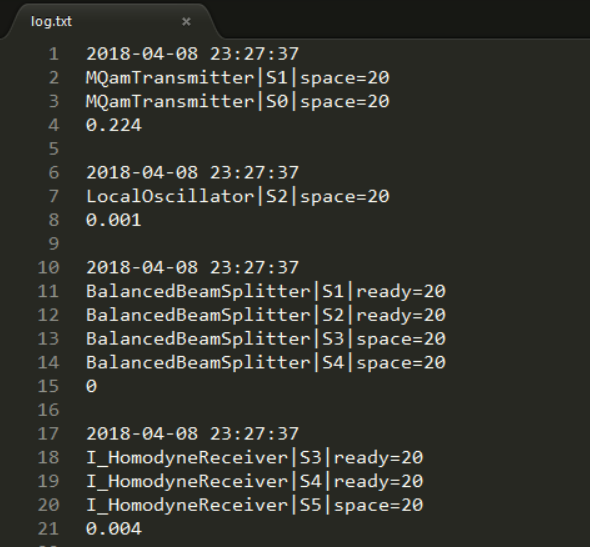
\includegraphics[width=.35\linewidth]{./chapter/simulator_structure/figures/output_file}
\caption{Output File Example}
\label{fig:outputfile}
\end{figure}

Figure \ref{fig:homodynesignals} shows a portion of code that consists in the declaration and inicialization of the I\_HomodyneReceiver block. In line 97, we can see that the block has 2 input signals, $S3$ and $S4$, and is assigned 1 output signal, $S5$. Going back to Figure \ref{fig:outputfile} we can observe that $S3$ and $S4$ have 20 samples ready to be processed and the buffer of $S5$ is empty.

\renewcommand{\figurename}{Figure}
\begin{figure}[H]
\centering
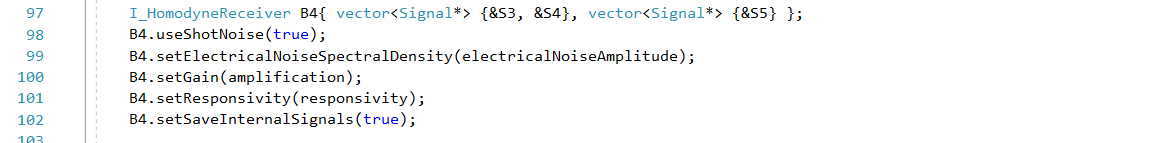
\includegraphics[width=1.3\linewidth]{./chapter/simulator_structure/figures/homodyne_signals}
\caption{I-Homodyne Receiver Block Declaration}
\label{fig:homodynesignals}
\end{figure}

\subsection{Testing Log File}
In directory \textit{doc/tex/chapter/simulator\_structure/test\_log\_file/bpsk\_system/} there is a copy of the BPSK system. You may use it to test the Log File. The main method is located in file \textit{bpsk\_system\_sdf.cpp}

% bibliographic references for the section ----------------------------
\clearpage
\printbibliography[heading=subbibliography]
\end{refsection}
\addcontentsline{toc}{subsection}{Bibliography}
\cleardoublepage
% ---------------------------------------------------------------------



%\include{chapter/development_cycle}
%\include{chapter/visualizer}

% ------------------------------------------------------------------------
\chapter{Case Studies}

\ifdefined\qpsk         \input{./sdf/qpsk_transmitter/qpsk_transmitter} \fi
\ifdefined\optical      \input{./sdf/optical_detection/optical_detection} \fi
\ifdefined\bpsk         \input{./sdf/bpsk_system/bpsk_system} \fi
\ifdefined\mQAM         \input{./sdf/m_qam_system/m_qam_system} \fi
\ifdefined\sdf          \input{./sdf/simplified_coherent_receiver/simplified_coherent_receiver} \fi
\ifdefined\rofKK        \input{./sdf/radio_over_fiber_with_kramers_kronig/radio_over_fiber_with_kramers_kronig} \fi
\ifdefined\dsp          \input{./sdf/dsp_laser_phase_compensation/dsp_laser_phase_compensation} \fi
\ifdefined\quantumRNG   \clearpage
\section{Quantum Random Number Generator}

\begin{refsection}

\begin{tcolorbox}	
\begin{tabular}{p{2.75cm} p{0.2cm} p{10.5cm}} 	
\textbf{Students Name}  &:& Mariana Ramos (12/01/2018 - )\\
\textbf{Goal}          &:& Simulate and implement an experimental setup of a Quantum Random Number Generator.\\
\textbf{Directory}          &:& sdf/quantum\_random\_number\_generator.
\end{tabular}
\end{tcolorbox}

True random numbers are indispensable in the field of cryptography \cite{Katsoprinakis08}. There are two approaches for random number generation: the pseudorandom generation which are based on an algorithm implemented on a computer, and the physical random generators which consist in measuring some physical observable with random behaviour. Since classical physics description is deterministic, all classical processes are in principle predictable. Therefore, a true random number generator must be based on a quantum process \cite{Jennewein00}.

In this chapter, it is presented the theoretical, the simulation and the experimental analysis of a quantum random generator based on the use of single photons linearly polarized at $45^{\circ}$.

\subsection{Theoretical Analysis}

One of the optical processes available as a source of randomness is the splitting of a polarized single photon beam. The principle of operation of the random generator is shown in figure \ref{qrng}. Each individual photon coming from the source is linearly polarized at $45^\circ$ and has equal probability of be found in the horizontal (H) or in the vertical (V) output of the PBS. Quantum theory estimates for both cases that the individual choices are truly random, independent one from each other , and with a probability of 1/2.

\begin{figure}[H]
    \centering
        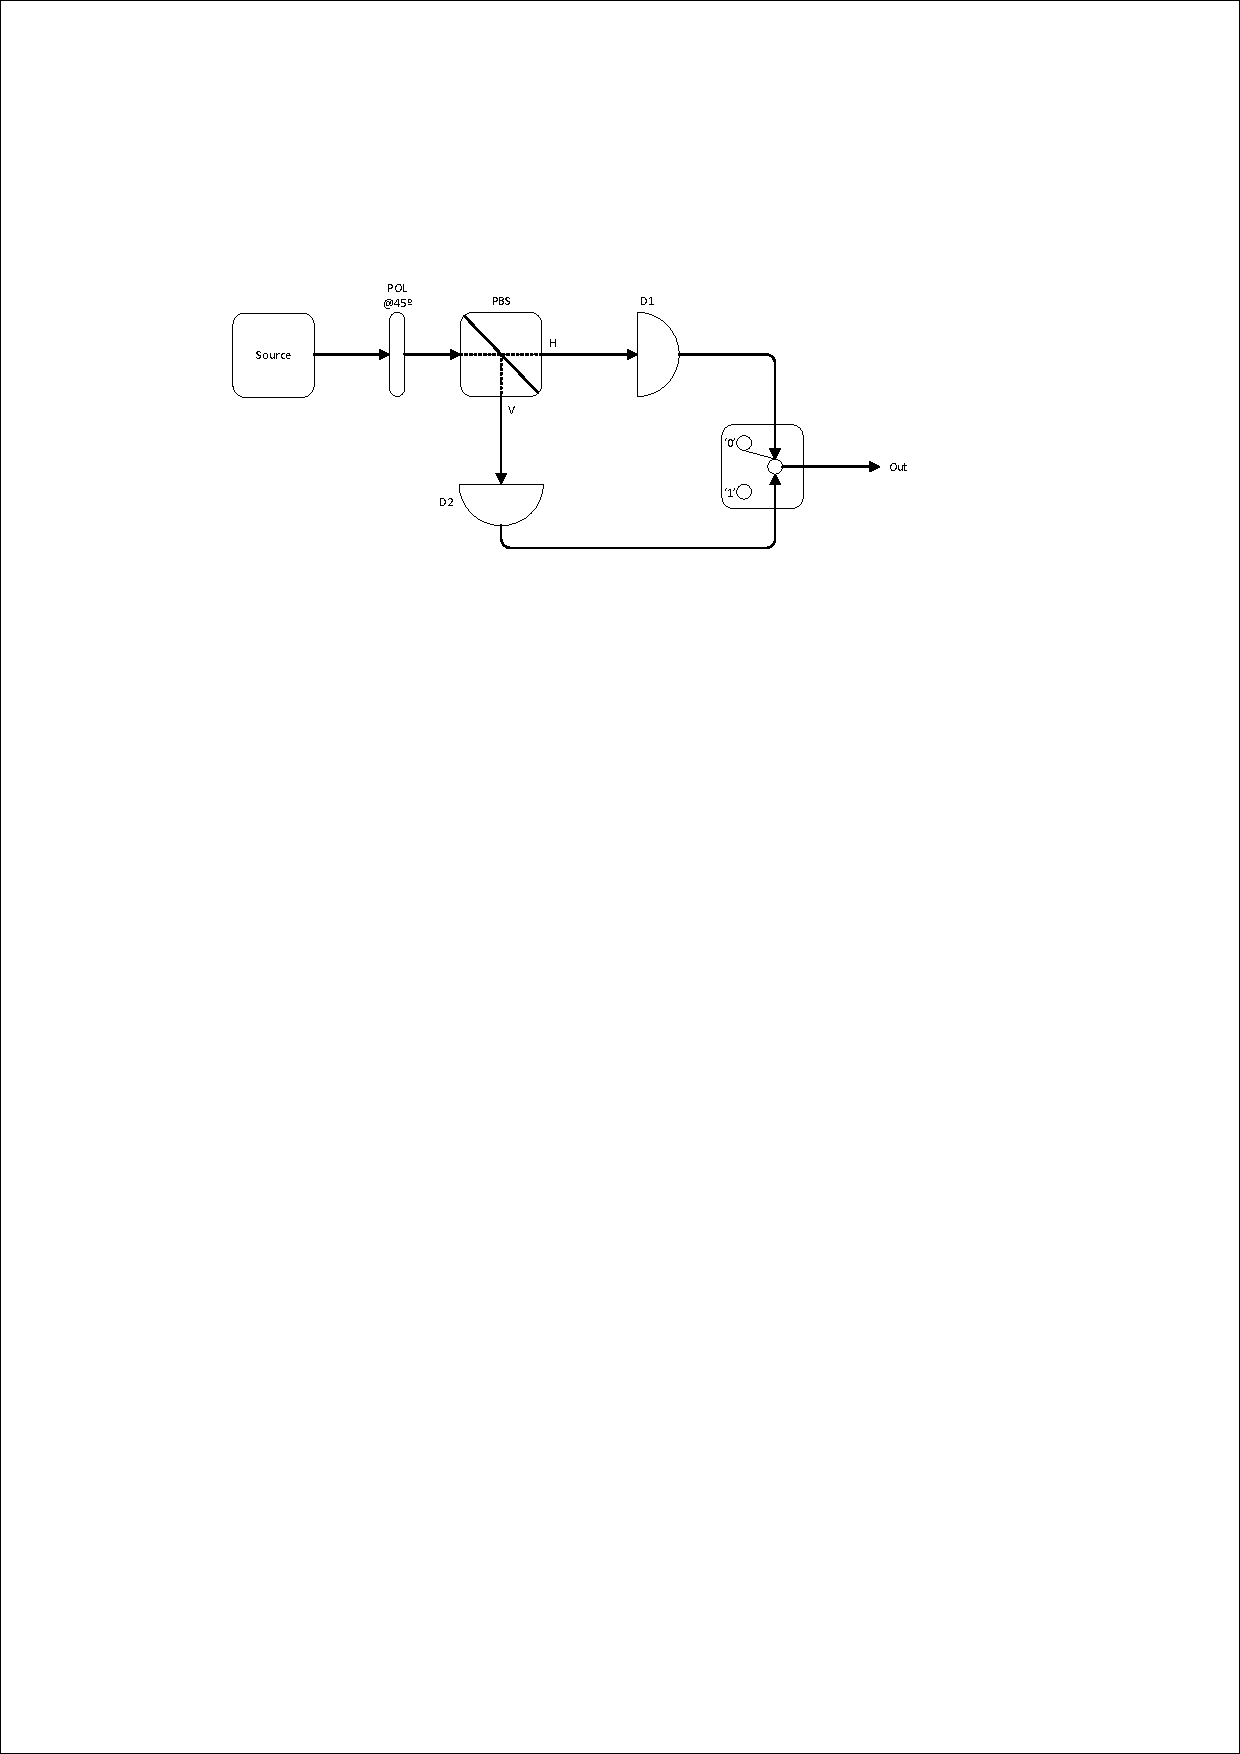
\includegraphics[clip, trim=3cm 20cm 5cm 5cm, width=1.00\textwidth]{./sdf/quantum_random_number_generator/figures/Random_Number_Generator.pdf}
    \caption{Source of randomness with a polarization beam splitter PBS where the incoming light is linearly polarized at $45^{\circ}$ with respect to the PBS. Figure adapted from \cite{Jennewein00}.}\label{qrng}
\end{figure}

From a classical approach, the information is stored as binary bits that can take the logical value '0' or '1'. From a quantum approach, the information can be stored in quantum bits or qubits for short. As a consequence of the superposition principle of quantum mechanics, qubits can not only represent the pure '0' or '1' states, but they can also represent a superposition of both. This way, qubits are governed by a quantum wave function $\psi$. Lets use the Dirac notation to represent the general state of the qubit:
\begin{equation}\label{eq:qubit}
  |\psi\rangle = C_0 |0\rangle + C_1 |1\rangle,
\end{equation}

and the normalization condition of $|\psi\rangle$ requires that $|C_0|^2+|C_1|^2=1$. This way, the relative proportion of each of the binary states on a qubit is governed by the amplitude coefficients $C_0$ and $C_1$. In the present example, we consider a linear polarization in which the two possible states are orthogonal, such that: $\langle 0|1 \rangle=0$. We define the $|0\rangle$ and $|1\rangle$ states to correspond to the horizontal and vertical polarization states, respectively:

\begin{eqnarray}
 %\nonumber % Remove numbering (before each equation)
  |\psi\rangle &=& C_0 |0\rangle+C_1 |1\rangle \\
             &=& C_0 |0^{\circ}\rangle + C_1 |90^{\circ}\rangle .
\end{eqnarray}

Amplitude coefficients $C_0$ and $C_1$ store the quantum information. Therefore, if one makes a measurement, the result will be '0' with probability $|C_0|^2$ or '1' with probability $|C_1|^2$.
Moreover, the state of a single photon can be also described by a wave function as a column vector:

\begin{equation}\label{eq:wavefvector}
  |\psi\rangle = \binom{C_0}{C_1},
\end{equation}
which will be used in simulation analysis.

\begin{figure}[h]
    \centering
        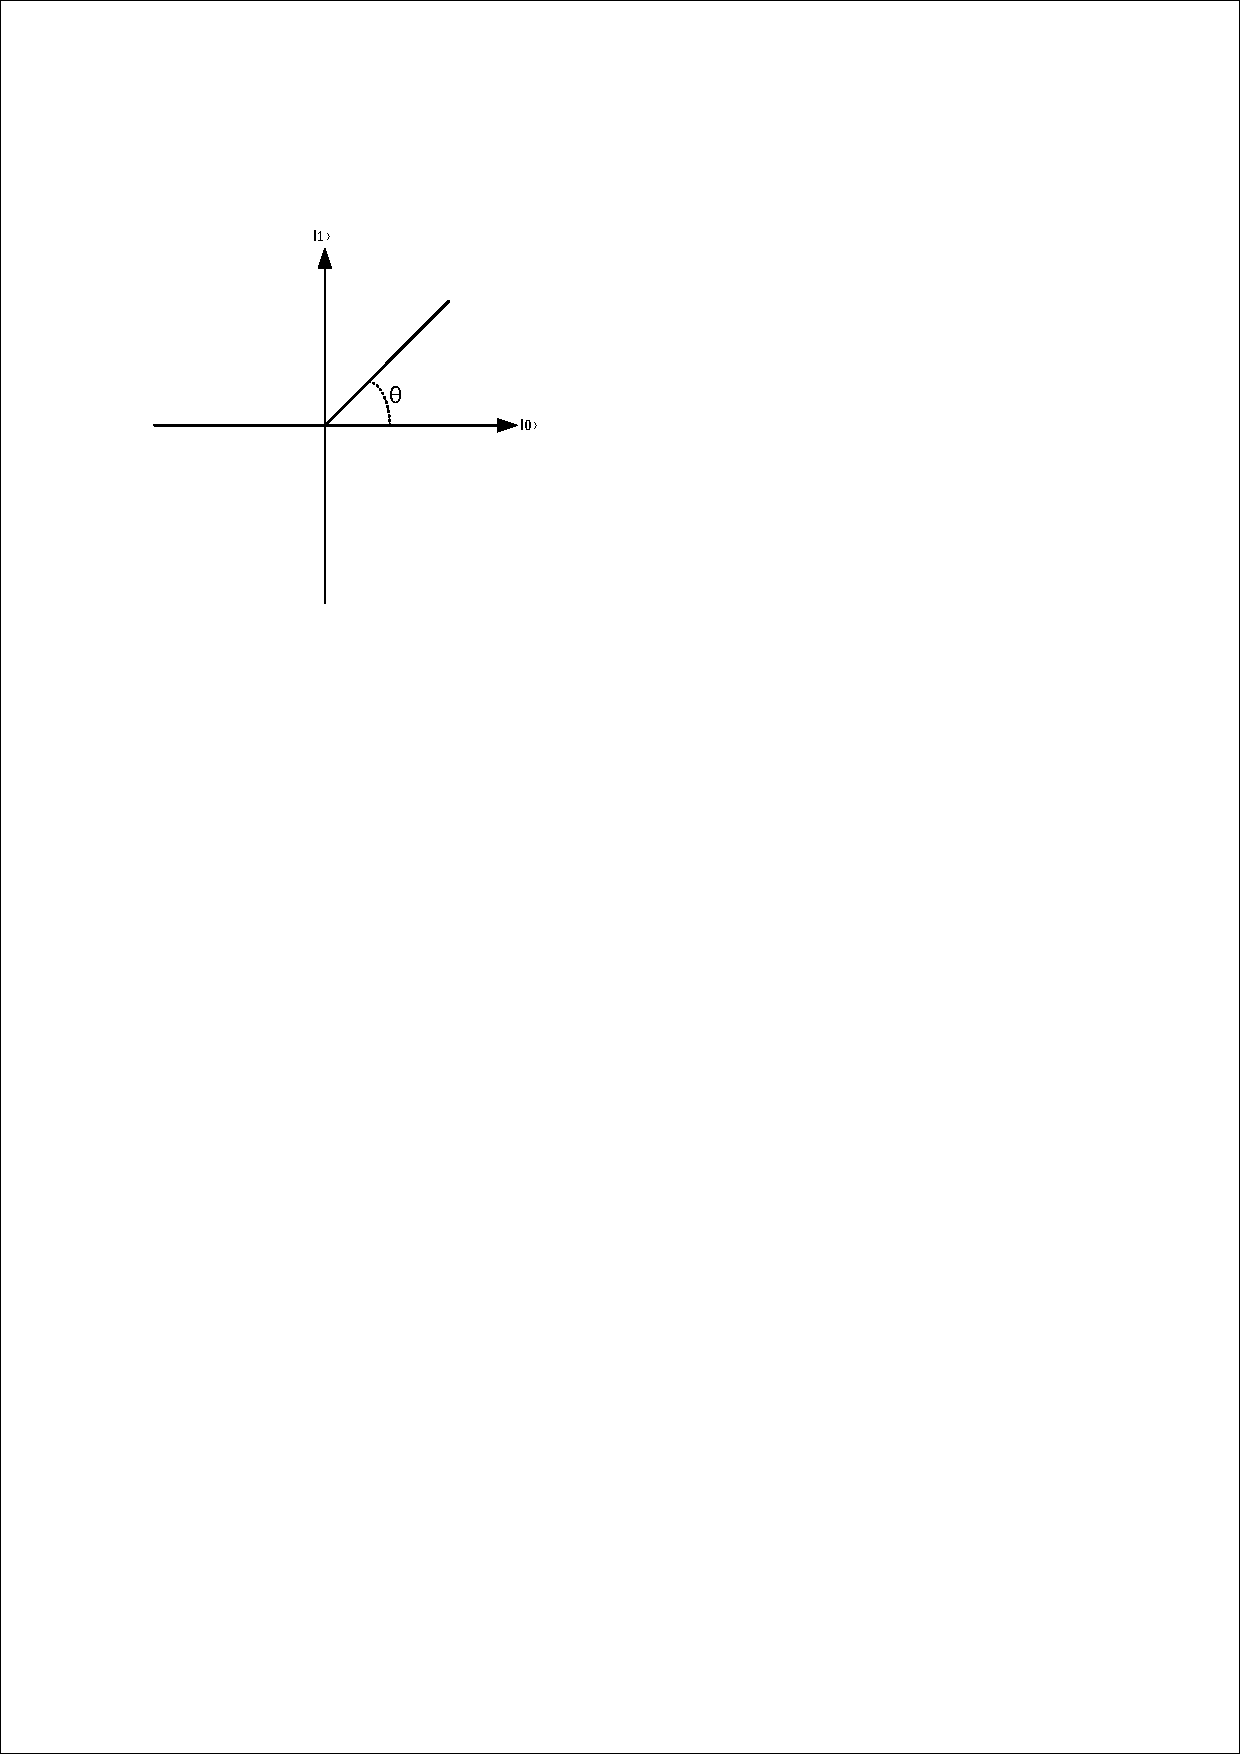
\includegraphics[clip, trim=3cm 20cm 12cm 3cm, height=6cm]{./sdf/quantum_random_number_generator/figures/axis_states.pdf}
    \caption{Representation of polarization states of a qubit in a bi-dimensional space.}\label{fig:stateaxis}
\end{figure}

As one can see in figure \ref{fig:stateaxis} the amplitude coefficients can be written as a function of $\theta$:
\begin{eqnarray}
% \nonumber % Remove numbering (before each equation)
  C_0 &=& cos(\theta) \\
  C_1 &=& sin(\theta).
\end{eqnarray}

According with the setup presented in figure \ref{qrng} and considering the polarization angle $\theta = 45^{\circ}$, the single photon has the probability of reach \textbf{D1} and outputs a "$0$" is equals to $|cos(\theta)|^2$ and the probability of reach \textbf{D2} and outputs a "$1$" is equals to $|sin(\theta)|^2$, which in the case $\theta = 45^{\circ}$ both have the same value equals to $0.5$.

\subsection{Simulation Analysis}
The simulation diagram of the setup described in the previous section is presented in figure \ref{sim_qrng}. The linear polarizer has an input control signal (S1) which allows to change the rotation angle. Nevertheless, the only purpose is to generate a time and amplitude continuous real signal with the value of the rotation angle in degrees. In addition, the photons are generated by single photon source block at a rate defined by the clock rate. At the end of the simulation there is a circuit decision block which will outputs a binary signal with value "$0$" \space if the detector at the end of the horizontal path clicks or "$1$" \space if the detector at the end of the vertical path clicks.

\begin{figure}[h]
    \centering
        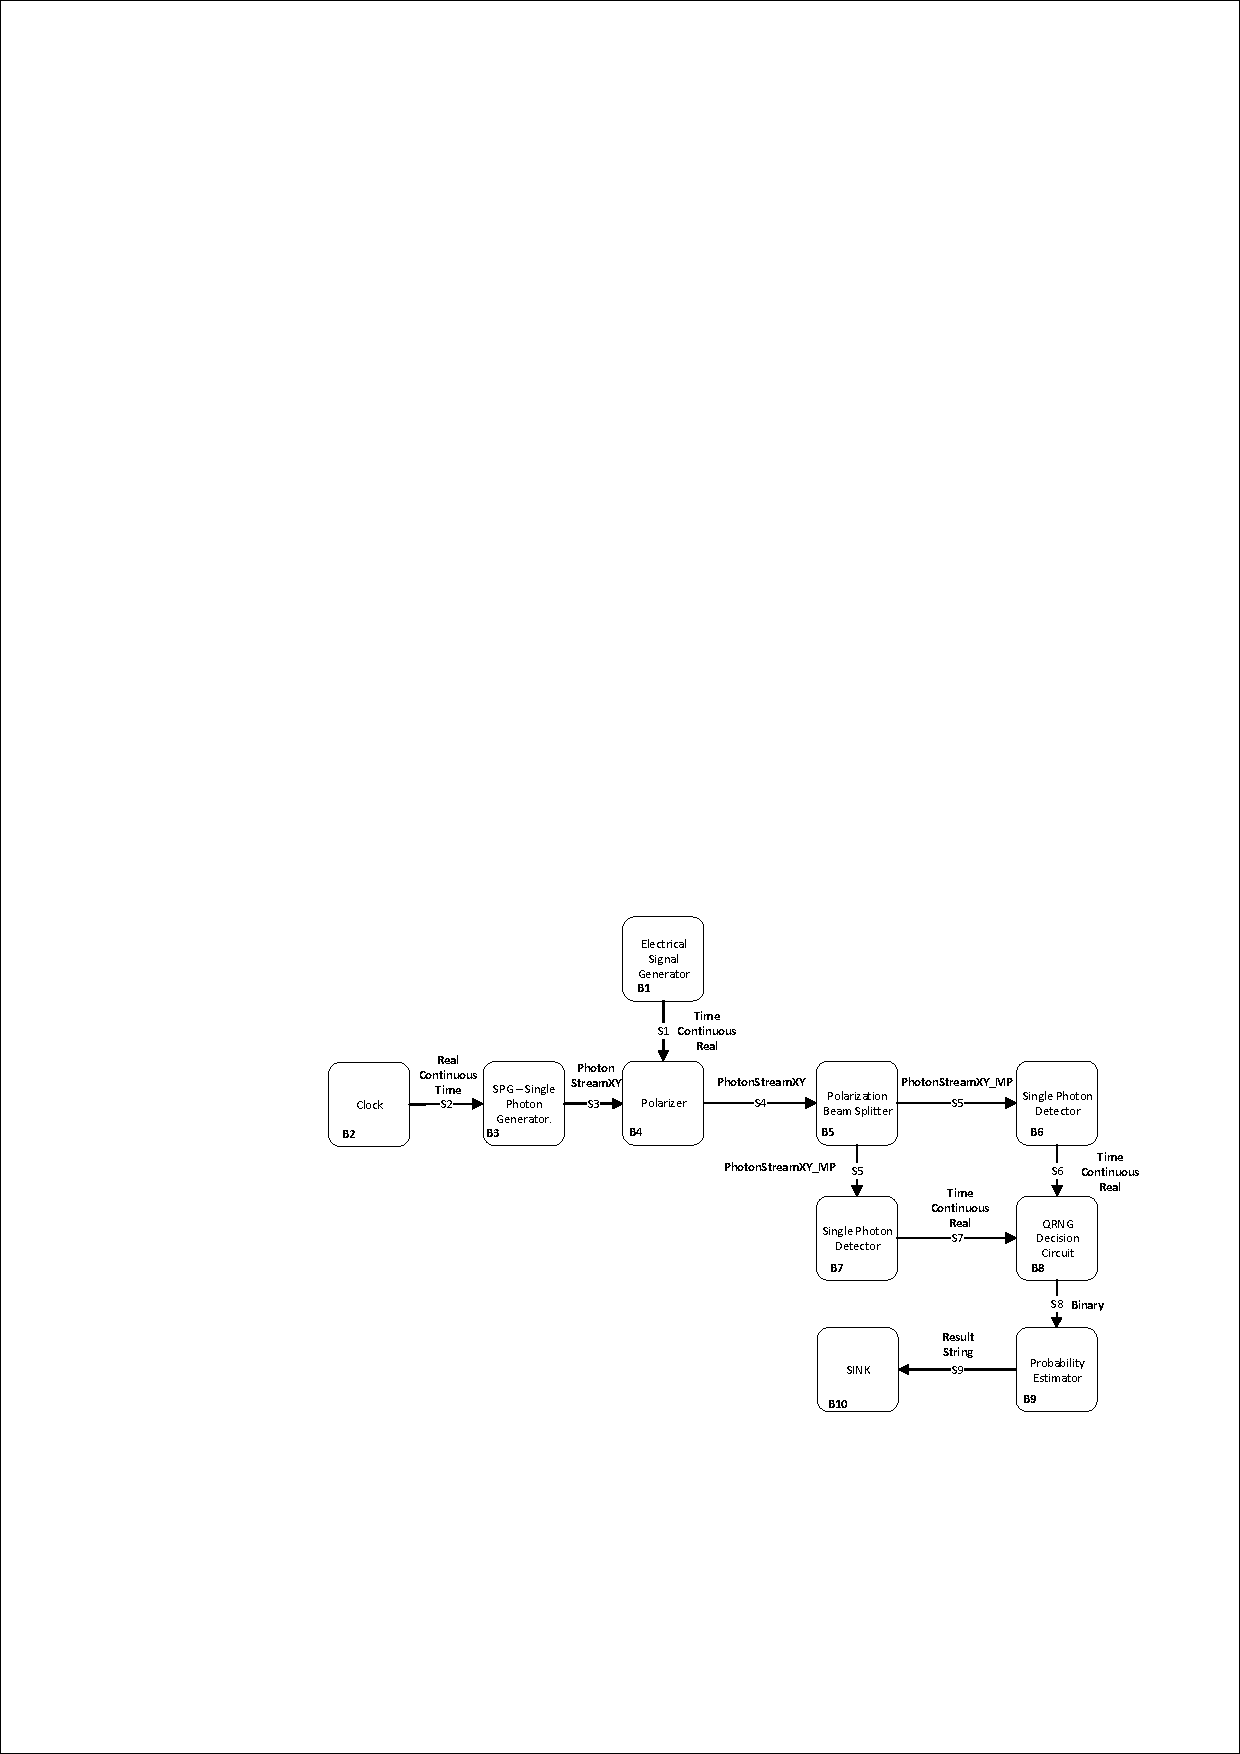
\includegraphics[clip, trim=5cm 5cm 0.5cm 15cm, width=1.00\textwidth]{./sdf/quantum_random_number_generator/figures/Simulation_qrng.pdf}
    \caption{Block diagram of the simulation of a Quantum Random Generator.}\label{sim_qrng}
\end{figure}

In table \ref{tb:inputparameters2} are presented the input parameters of the system.


\begin{table}[H]
\centering
\caption{System Input Parameters}
\label{tb:inputparameters2}
\begin{tabular}{|c|c|c|}
\hline
\textbf{Parameter}                      & \textbf{Default Value}                                       \\ \hline
RateOfPhotons                           & 1e6                                                          \\ \hline
NumberOfSamplesPerSymbol                & 16                                                           \\ \hline
PolarizerAngle                          & 45.0                                                         \\ \hline

\end{tabular}
\end{table}

In table \ref{tb:signals2} are presented the system signals to implement the simulation presented in figure \ref{sim_qrng}.
\begin{table}[H]
\centering
\caption{System Signals}
\label{tb:signals2}
\begin{tabular}{|c|c|c|}
\hline
\textbf{Signal name}                            & \textbf{Signal type}                      \\ \hline
S1                                              &  TimeContinuousAmplitudeContinuousReal    \\ \hline
S2                                              &  TimeContinuousAmplitudeContinuousReal    \\ \hline
S3                                              &  PhotonStreamXY                           \\ \hline
S4                                              &  PhotonStreamXY                           \\ \hline
S5                                              &  PhotonStreamXYMP                         \\ \hline
S6                                              &  TimeContinuousAmplitudeContinuousReal    \\ \hline
S7                                              &  TimeContinuousAmplitudeContinuousReal    \\ \hline
S8                                              &  Binary                                   \\ \hline
S9                                              &  Binary                                   \\ \hline
\end{tabular}
\end{table}

Table \ref{tb:signalsh} presents the header files used to implement the simulation as well as the specific parameters that should be set in each block. Finally, table \ref{tb:signalss} presents the source files.

\begin{table}[H]
\centering
\caption{Header Files}
\label{tb:signalsh}
\begin{tabular}{|c|c|c|}
\hline
\textbf{File name}                              & \textbf{Description}                                                          & \textbf{Status} \\ \hline
netxpto\_20180118.h                             &                                                                               &    \checkmark   \\ \hline
electrical\_signal\_generator\_20180124.h       &setFunction(), setGain()                                                       &    \checkmark   \\ \hline
clock\_20171219.h                               &ClockPeriod(1 / RateOfPhotons)                                                 &    \checkmark   \\ \hline
polarization\_beam\_splitter\_20180109.h        &                                                                               &   \checkmark   \\ \hline
polarizer\_20180113.h                           &                                                                               &    \checkmark   \\ \hline
single\_photon\_detector\_20180111.h            &setPath(0), setPath(1)                                                         &    \checkmark   \\ \hline
single\_photon\_source\_20171218.h              &                                                                               &    \checkmark   \\ \hline
probability\_estimator\_20180124.h              &                                                                               &    \checkmark   \\ \hline
sink.h                                          &                                                                               &    \checkmark   \\ \hline
qrng\_decision\_circuit.h                       &                                                                               &    \checkmark   \\ \hline
\end{tabular}
\end{table}

\begin{table}[H]
\centering
\caption{Source Files}
\label{tb:signalss}
\begin{tabular}{|c|c|c|}
\hline
\textbf{File name}                              & \textbf{Description} & \textbf{Status} \\ \hline
netxpto\_20180118.cpp                           &                      &    \checkmark   \\ \hline
electrical\_signal\_generator\_20180124.cpp     &                      &    \checkmark   \\ \hline
clock\_20171219.cpp                             &                      &    \checkmark   \\ \hline
polarization\_beam\_splitter\_20180109.cpp      &                      &   \checkmark   \\ \hline
polarizer\_20180113.cpp                         &                      &    \checkmark   \\ \hline
single\_photon\_detector\_20180111.cpp          &                      &    \checkmark   \\ \hline
single\_photon\_source\_20171218.cpp            &                      &    \checkmark   \\ \hline
probability\_estimator\_20180124.cpp            &                      &    \checkmark   \\ \hline
sink.cpp                                        &                      &    \checkmark   \\ \hline
qrng\_decision\_circuit.cpp                     &                      &    \checkmark   \\ \hline
qrng\_sdf.cpp                                   &                      &    \checkmark   \\ \hline
\end{tabular}
\end{table}

 Lets assume, for an angle of $45^{\circ}$, a number of samples$N=1 \times 10^{6}$ and the expected probability of reach each detector of $\hat{p} = 0.5$. We have an error margin of $E = 1.288 \times 10 ^{-3}$, which is acceptable. This way, the simulation will be performed for $N=1 \times 10^{6}$ samples for different angles of polarization shown in figure \ref{sphere} with different error margin's values since the expected probability changes depending on the polarization angle.

\begin{figure}[H]
    \centering
        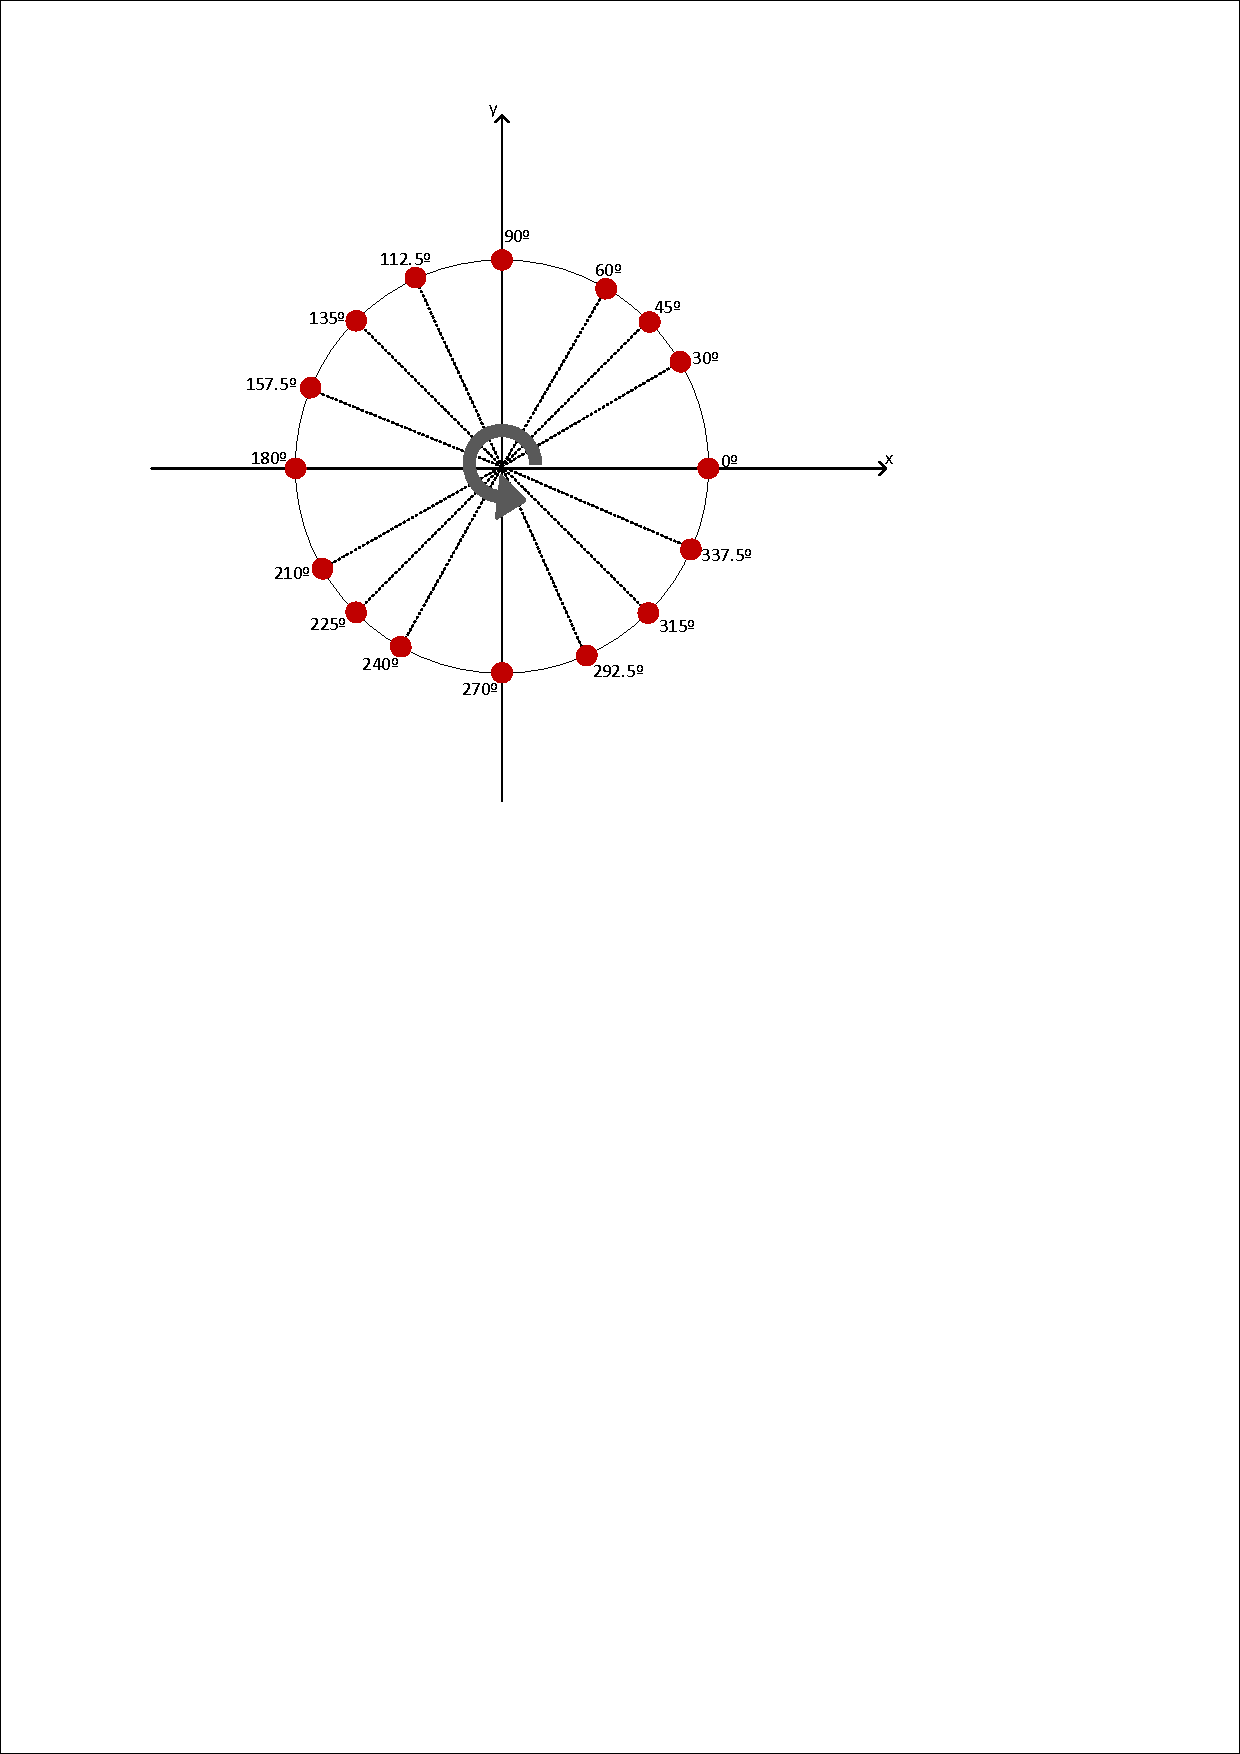
\includegraphics[clip, trim=0.5cm 15.5cm 2.5cm 1cm, height = 10cm]{./sdf/quantum_random_number_generator/figures/sphere.pdf}
    \caption{Angles used to perform the qrng simulation for $N=1 \times 10^{6}$ samples. }\label{sphere}
\end{figure}

For a quantum random number generator with equal probability of obtain a "0" \space or "1" \space the polarizer must be set at $45^{\circ}$. This way, we have $50\%$ possibilities to obtain a "0" \space and $50\%$ of possibilities to obtain a "1" \space. This theoretical value meets the value obtained from the simulation when it is performed for the number of samples mentioned above.

\begin{figure}[H]
    \centering
        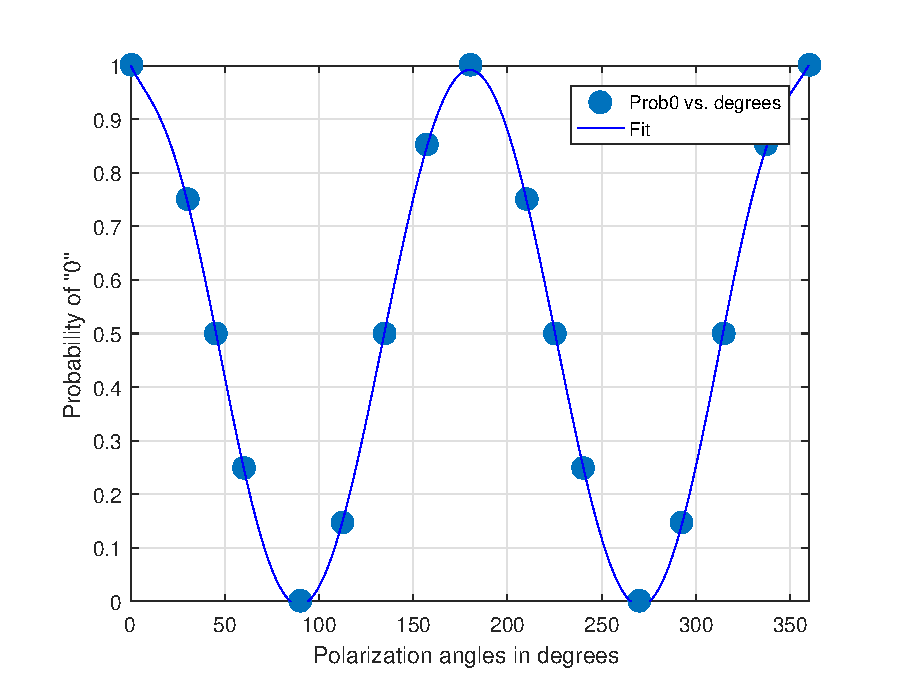
\includegraphics[width=15cm,height=10cm]{./sdf/quantum_random_number_generator/figures/prob0.eps}
    \caption{Probability of outputs a number "0" \space depending on the polarization angle.}\label{probx}
\end{figure}

Figure \ref{probx} shows the probability of a single photons reaches the detector placed on Horizontal axis depending on the polarization angle of the photon, and this way the output number is "0". The following table shows the goodness of the fit:
\begin{table}[H]
\centering
\label{tab:goodnessfitprob0}
    \begin{tabular}{c|c}
      SSE:                  & 0.0004785\\
      R-square:             &0.9998\\
      Adjusted R-square:    &0.9995\\
      RMSE:                 &0.007734
  \end{tabular}
\end{table}

On the other hand, figure \ref{proby} shows the probability of a single photon reaches the detector placed on Vertical component of the polarization beam splitter, and this way the output number is "1". As we can see in the figures the two detectors have complementary probabilities, i.e the summation of both values must be equals to $1$. One can see that "Probability of $1$" \space behaves almost like a sine function and "Probability of 0" \space behaves almost like a cosine function with a variable angle.

\begin{figure}[H]
    \centering
        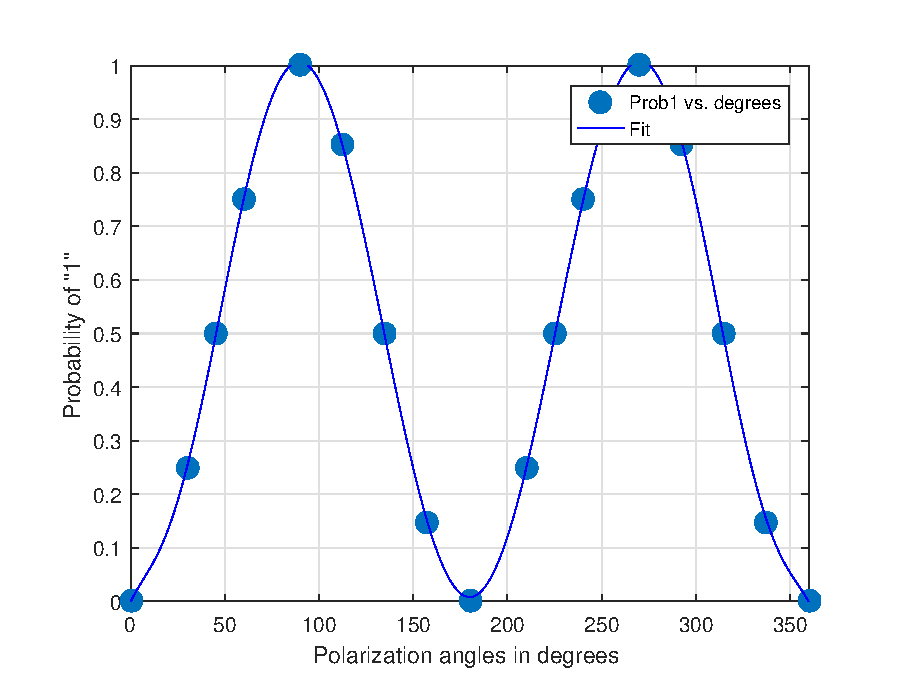
\includegraphics[width=15cm,height=10cm]{./sdf/quantum_random_number_generator/figures/prob1.eps}
    \caption{Probability of outputs a number "1" \space depending on the polarization angle.}\label{proby}
\end{figure}

The goodness of the fit presented in figure \ref{proby} is shown in the following table:
\begin{table}[H]
\centering
\label{tab:goodnessfitprob0}
    \begin{tabular}{c|c}
        SSE:                &0.0004785\\
        R-square:           &0.9998\\
        Adjusted R-square:  &0.9995\\
        RMSE:               &0.007734
  \end{tabular}
\end{table}

The goodness of the fit is evaluated based on four parameters:
\begin{enumerate}
  \item The sum of squares due to error (SSE), which measures the total deviation between the fit values and the values that the simulation outputs. This value is calculated from the expression
      \begin{equation}\label{}
        \textrm{SSE} = \sum_{i=1}^{n} w_i(y_{i}-\hat{y_{i}})^2.
        \nonumber
      \end{equation}
      A value of SSE closer to 0 means that the model has a small random error component.

  \item The R-square measures how good the fit in explaining the data.
    \begin{equation}\label{}
    \textrm{R-square} = 1-\frac{\textrm{SSE}}{\textrm{SST}},
    \nonumber
    \end{equation}
    where,
    \begin{equation}\label{}
    \textrm{SST} = \sum_{i=1}^{n} w_i (y_i - \bar{y_i})^2.
      \nonumber
    \end{equation}
    R-square can take a value between 0 and 1. If the value is closer to 1, it means that the fit better explains the total variation in the data around the average.

  \item Degrees of freedom adjusted R-square uses the R-square and adjusts it based on the number of degrees of freedom.
    \begin{equation}\label{}
      \textrm{adjusted R-square} = 1 - \frac{\textrm{SSE}(n-1)}{\textrm{SST}(v)},
      \nonumber
    \end{equation}
    where,
    \begin{equation}\label{}
      v = n - m,
      \nonumber
    \end{equation}
    where n is the number of values in test and m is the number of fitted coefficients estimated from the values in test. A value of adjusted R-square close to 1 is a indicative factor of a good fit.

  \item The root mean square error (RMSE) is also a fit standard error and it can be calculated from:
    \begin{equation}\label{}
      \textrm{RMSE} = \sqrt{\textrm{MSE}},
      \nonumber
    \end{equation}
    where,
    \begin{equation}\label{}
      \textrm{MSE} = \frac{\textrm{SSE}}{v}.
      \nonumber
    \end{equation}

\end{enumerate}

\subsection{Experimental Analysis}

In order to have a real experimental quantum random number generator, a setup shown in figure \ref{experimental_qrng} was built in the lab. To simulate a single photon source we have a CW-Pump laser with $1550$ nm wavelength followed by an interferometer Mach-Zenhder in order to have a pulsed beam. The interferometer has an input signal given by a Pulse Pattern Generator. This device also gives a clock signal for the Single Photon Detector (APD-Avalanche Photodiode) which sets the time during which the window of the detector is open. After the MZM there is a Variable Optical Attenuator (VOA) which reduces the amplitude of each pulse until the probability of one photon per pulse is achieved. Next, there is a polarizer controller followed by a Linear Polarized, which is set at $45^{\circ}$, then a Polarization Beam Splitter (PBS) and finally, one detector at the end of each output of the PBS. The output signals from the detector will be received by a Processing Unit. Regarding to acquired the output of the detectors, there is an oscilloscope capable of record $1 \times 10^{6}$ samples.



\begin{figure}[H]
    \centering
        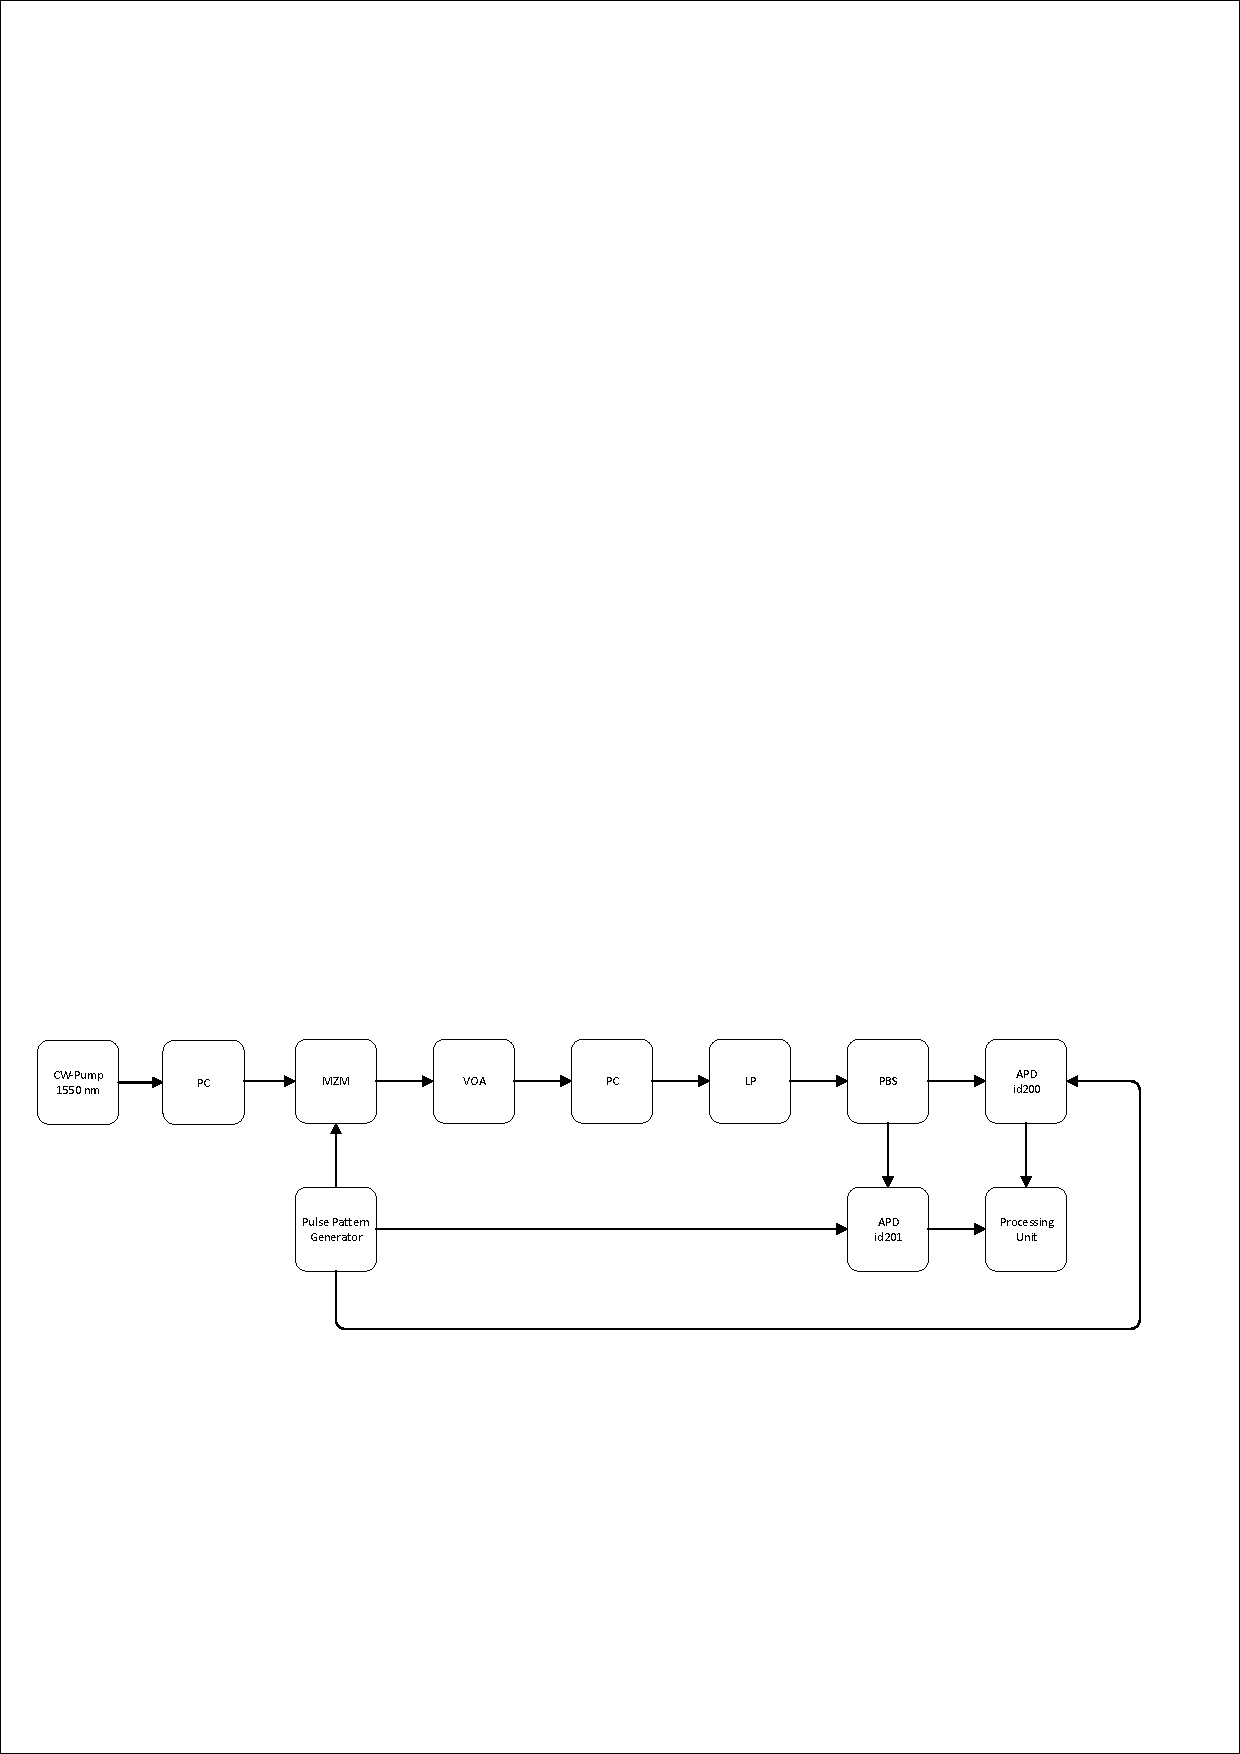
\includegraphics[clip, trim=0.5cm 7cm 0.5cm 17cm, width=1.00\textwidth]{./sdf/quantum_random_number_generator/figures/experimental_qrng.pdf}
    \caption{Experimental setup to implement a quantum random number generator.}\label{experimental_qrng}
\end{figure}

\subsubsection{IDQuantique detector}
%
The detector used in the laboratory is the Thorlabs PDB 450C. This detector consists of two well-matched photodiodes and a transimpedance amplifier that generates an output voltage (RF OUTPUT) proportional to the difference between the photocurrents of the photodiodes.\\
Additionally, the unit has two monitor outputs (MONITOR+ and MONITOR-) to observe the optical input power level on each photodiode separately.

Since we do not have a single photon source, we must use the Poisson Statistics in order to calculate the best value for a mean of photons per pulse. A weak laser pulse follows a Poissonian Statistics\cite{Fox06}:
\begin{equation}\label{eq:poisson}
  S_n = e^{-\mu}\frac{\mu^{n}}{n!},
\end{equation}
where $\mu$ is the average photon number. In addition, the probability of an optical pulse carries one photon at least is:
\begin{equation}\label{eq:prob1photon}
  P = 1 - S_0 = 1 - e^{-\mu}.
\end{equation}

On the other hand, the probability of a detector clicks is:

\begin{equation}\label{eq:detectorclickprob}
  P_{click} = P_{det}+P_{dc} + P_{det}P_{dc},
\end{equation}

where $P_{det}$ is the probability of the detector clicks due a photon which cross its window and $P_{dc}$ is the probability of dark counts. Considering the detector efficiency $\eta_{D}$, the probability of the detector clicks due to a photon is:

\begin{equation}\label{eq:probclickefficiency}
  P_{det} = 1 - e^{- \eta_{D}\mu}.
\end{equation}

The probability of dark counts is calculated as a ratio between the frequency counts and the trigger frequency when no laser is connected to the detector. Nevertheless, the detector click frequency is
\begin{equation}\label{eq:frequencyclick}
  f_{click} = f_{trigger}P_{click} \longrightarrow P_{click}=\frac{f_{click}}{f_{trigger}}.
\end{equation}

This way the mean average photon number can be calculate using the following equation:
\begin{equation}\label{eq:meanphotonnumber}
  \mu = - \frac{1}{\eta_{D}}\ln\left [1-\frac{1}{1-P_{dc}}\left (\frac{f_{click}}{f_{trigger}}-P_{dc} \right)\right]
\end{equation}

\subsection{Open Issues}

\newpage


% bibliographic references for the section ----------------------------
\clearpage
\printbibliography[heading=subbibliography]
\end{refsection}
\addcontentsline{toc}{subsection}{Bibliography}
\cleardoublepage
% ---------------------------------------------------------------------  \fi
\ifdefined\bb           \clearpage
\section{BB84 with Discrete Variables}

\begin{refsection}

\begin{tcolorbox}	
\begin{tabular}{p{2.75cm} p{0.2cm} p{10.5cm}} 	
\textbf{Students Name}  &:& Mariana Ramos (7/11/2017 - 9/4/2018) \\
                        & & Kevin Filipe (7/11/2017 - 10/11/2017) \\
\textbf{Starting Date} &:& November 7, 2017\\
\textbf{Goal}          &:& BB84 implementation with discrete variables.
\end{tabular}
\end{tcolorbox}

BB84 is a key distribution protocol which involves three parties, Alice, Bob and Eve. Alice and Bob exchange information between each other by using a quantum channel and a classical channel. The main goal is continuously build keys only known by Alice and Bob, and guarantee that eavesdropper, Eve, does not gain any information about the keys.


\subsection{Protocol Analysis}
\begin{tcolorbox}	
	\begin{tabular}{p{2.75cm} p{0.2cm} p{10.5cm}} 	
		\textbf{Students Name}  &:& Kevin Filipe (7/11/2017 - 10/11/2017)\\
		\textbf{Goal}          &:& BB84 - Protocol Description
	\end{tabular}
\end{tcolorbox}

BB84 protocol was created by Charles Bennett and Gilles Brassard in 1984 \cite{Bennet84}. It involves two parties, Alice and Bob, sharing keys through a quantum channel in which could be accessed by a eavesdropper, Eve. A basic model is depicted in figure \ref{fig:qkd model}.

\begin{figure}[H]
	\centering
	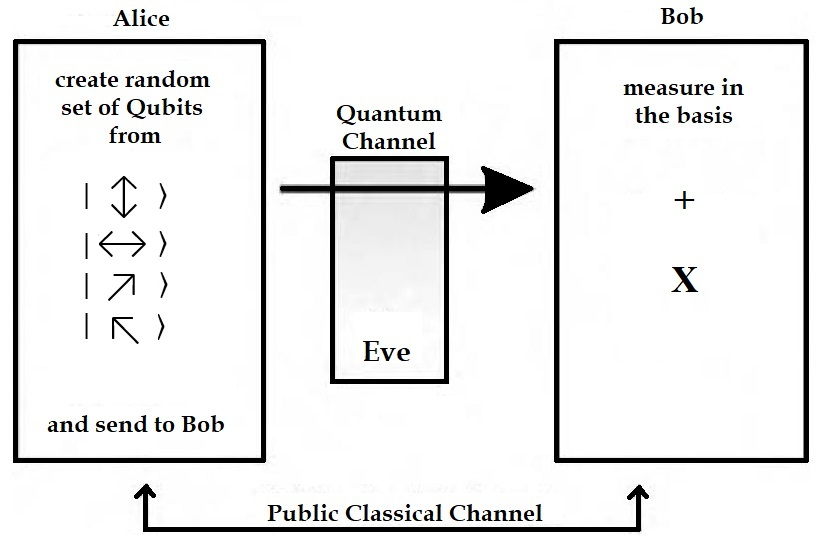
\includegraphics[width=0.8\textwidth,height=7cm]{./sdf/bb84_with_discrete_variables/figures/QKD_Model.png}
	\caption{Basic QKD Model. Alice and Bob are connected by 2 communication channels, a public quantum channel and a authenticated classical channel, with an eavesdropper, Eve (figure adapted from \cite{Gerry05}).}\label{fig:qkd model}
\end{figure}

We are going to analyse the BB84 protocol with bit encoding into photon state polarization. Two non-orthogonal basis are used to encode the information, the rectilinear and diagonal basis, + and x respectively. The following table shows this bit encoding.
\begin{table}[H]
	\centering
	\begin{tabular}{c|c|c}
		 Bit &  \textit{Rectilinear Basis,+} & \textit{Diagonal Basis,$\times$}\\ \hline
		0 &  0$º$ & -45$º$ \\
		1 & 90$º$ & 45$º$\\
	\end{tabular}
\end{table}

The protocol requires the following parameter and it is implemented with the following steps:

\begin{table}[hbt]
	\centering
	\caption{Initial Parameters.}
	\label{tb:param}
	\begin{tabular}{|c|c|}
		\hline
		\textbf{Parameter}  & \textbf{Description} 	   \\ \hline
			$M \times N$    & Scrambling Matrix M by N \\ \hline
			k				& Number of revealed bits for BER calculation \\ \hline
			$\alpha$        & Confidence level 	       \\ \hline
			    A    & B                \\ \hline
	\end{tabular}
\end{table}

\begin{enumerate}
	\item Alice generates two random bit strings. The random string , $R_{A1}$, corresponds to the data to be encoded into photon state polarization. $R_{A2}$ is a random string in which 0 and 1 corresponds to the rectilinear, +, and diagonal, $\times$, respectively.
	
	$$ R_{A1} = \{0,1,1,0,1,0,0,1,1,0,1,1,1,0,0,1,0,0,0,1\}$$
	\begin{eqnarray}
		R_{A2} &=& \{0,0,1,0,1,1,1,0,1,1,1,0,1,0,0,0,1,0,1,0\} \nonumber \\
		&=& \{+,+,\times,+,\times, \times, \times, +,\times, \times, \times,+,\times,+,+,+,\times,+,\times,+\}\nonumber
	\end{eqnarray}
	
	\item Alice transmits a train of photons, $S_{AB}$, obtained by encoding the bits, $R_{A1}$ with the respective photon polarization state $R_{A2}$.
	
	$$S_{AB} = \{\to, \uparrow, \searrow, \to, \searrow, \nearrow, \nearrow, \uparrow, \searrow, \nearrow, \searrow, \uparrow, \searrow, \to, \to, \uparrow, \nearrow, \to, \nearrow, \uparrow\}.$$
	
	\item Bob generates a random string, $R_{B}$, to receive the photon trains with the correspondent basis.
	\begin{eqnarray}
		R_{B} &=& \{0,1,1,1,0,1,0,0,1,1,0,0,1,1,0,0,1,1,0,0\} \nonumber\\
		&=&\{+,\times,\times,\times,+,\times,+,+,\times,\times,+,+,\times,\times,+,+,\times,\times,+,+\} \nonumber
	\end{eqnarray}
	
	\item Bob performs the incoming photon states measurement, $M_{B}$, with its generated random basis, $R_{B}$. If the two photon detectors don't click, means the bit was lost during transference due to attenuation. If both photon detectors click, a false positive was detected. In the measurements, $M_{B}$, the no-click in both detectors is represented by a -1 and the false positives to -2. The measurements done in rectilinear or diagonal basis are represented by 0 or 1, respectively. This is represented \ref{fig:bb84 detector}
	
	$$M_{B} = \{0,1,1,1,-1,1,0,0,-2,1,0,0,-2,1,0,0,1,-1,0,0\}$$	

	\begin{figure}[H]
		\centering
		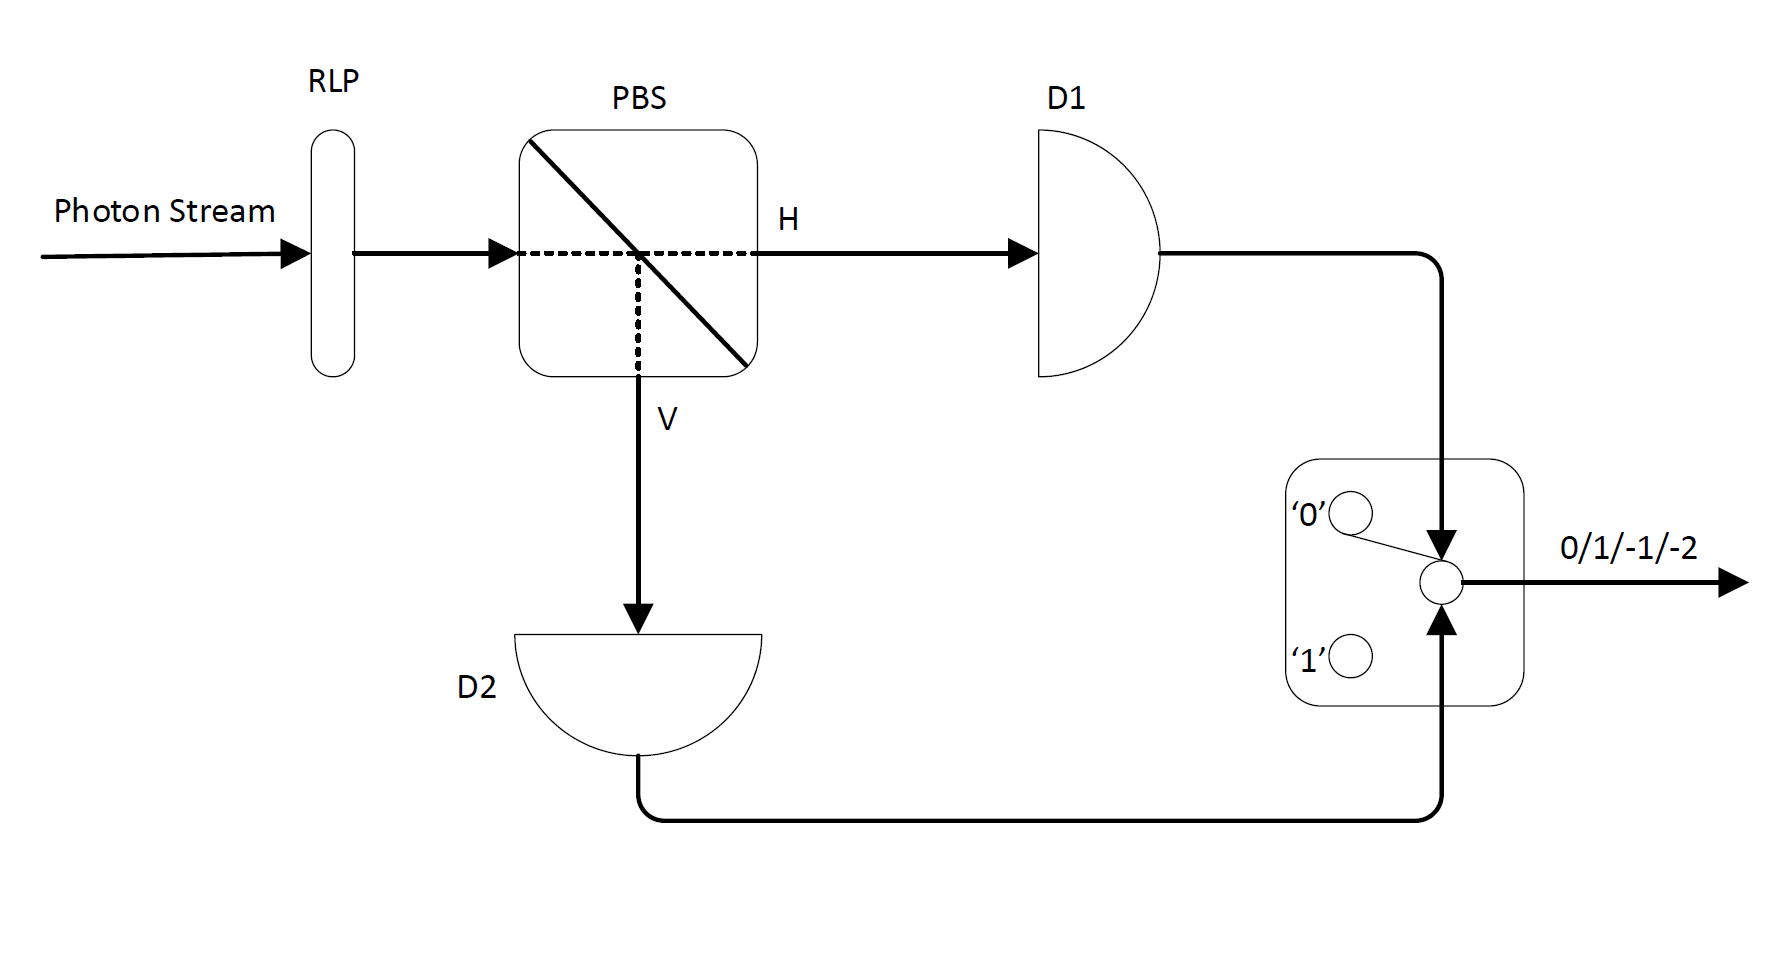
\includegraphics[width=0.8\textwidth,height=7cm]{./sdf/bb84_with_discrete_variables/figures/detector.png}
		\caption{Single-Photon Detection block with false-positives, -2, and attenuation, -1, detection depending on D1 and D2 output.\label{fig:bb84 detector}}
	\end{figure}
	
	\item After the measurement, Bob sends to Alice, using the classical channel, the used basis values, $R_{B}$ with the attenuation, -1, and false positives,-2.
	\item Alice performs a modified negated XOR, generating a sequence that detects when the same basis she used $B_{AB}$.
	
	\begin{table}[H]
		\centering
		\begin{tabular}{c|c c c c c c c c c c c c c c c c c c c c}
			$R_{A2}$ & 0 & 0 & 1 & 0 &  1 & 1 & 1 & 0 &  1 & 1 & 1 & 0 &  1 & 0 & 0 & 0 & 1 &  0 & 1 & 0 \\
			$R_{B}$  & 0 & 1 & 1 & 1 & -1 & 1 & 0 & 0 & -2 & 1 & 0 & 0 & -2 & 1 & 0 & 0 & 1 & -1 & 0 & 0 \\ \hline
			$B_{AB}$ & 1 & 0 & 1 & 0 &  0 & 1 & 0 & 1 &  0 & 1 & 0 & 1 &  0 & 0 & 1 & 1 & 1 &  0 & 0 & 1 \\
		\end{tabular}
	\end{table}

	\item Alice sends the $B_{AB}$ sequence to Bob, in which he can correlate with, $M_{B}$, and deduce the key $K_{AB}$.
	
			$$ K_{AB} = \{0,1,0,1,0,1,0,1,0,1\}.$$
	
	\item Alice then by having knowledge of $R_{A2}$ and $B_{AB}$ performs a scrambling algorithm over the deduced key. It is generated a matrix $M \times N$, according to the input parameter. Assuming a scrambling matrix of 3x4, \ref{tb:scram}. And being the scramble key represented as $KS_{AB}$
	
	\begin{table}[hbt]
		\centering
		\caption{Scrambling matrix}
		\label{tb:scram}
		\begin{tabular}{|c|c|c|c|c|}
			\hline
				0 & 1 & 0 & 1 \\ \hline
			    0 & 1 & 0 & 1 \\ \hline
				0 & 1 & - & - \\ \hline
		\end{tabular}
	\end{table}

	$$KS_{B} = \{0,0,0,1,1,1,0,0,1,1\}$$	
	
	\item Bob uses the same algorithm as Alice and scrambles his key.
	
	\item Bob then reveals a fixed number of his key to Alice. This number is also an input parameter value, k. With this the Quantum Bit Error Rate (QBER).
		
\end{enumerate}

	To determine the QBER, it is necessary to know the confidence interval parameter, $\alpha$ and the QBER limit, in which states the maximum allowed QBER by the user.
	Then to verify if the channel is reliable or not, the flowchart presented in figure \ref{fig:flowQber}.
	
	\begin{enumerate}
		\item Bob will reveals k bits sequence from the scrambled key, $SK_{AB}$ to Alice.
		\item Alice then returns to Bob the estimated QBER value, mQBER, with a confidence interval, [qLB, qUB] using the using the equations in the Bit Error Rate section, but applied to this protocol
		\item To check if the channel is compromised or not it is necessary to check if the QBER limit is higher than the QBER upper bound. If QBER limit is between the QBER lower and upper bound it is necessary to reveal more k bits from the key. Otherwise the channel is compromised and the key determination process needs to restart.
	\end{enumerate}
	
	
\begin{figure}[H]
	\centering
	\includegraphics[width=1\textwidth,height=7cm]{./sdf/bb84_with_discrete_variables/figures/qberEstimation.png}
	\caption{Flowchart to determine if the channel is reliable or not.}\label{fig:flowQber}
\end{figure}



\newpage

\subsection{Simulation Analysis}

\begin{tcolorbox}	
\begin{tabular}{p{2.75cm} p{0.2cm} p{10.5cm}} 	
\textbf{Students Name}  &:& Mariana Ramos (7/11/2017 - 9/4/2018) \\
\textbf{Goal}          &:& Perform a simulation of BB84 communication protocol.
\end{tabular}
\end{tcolorbox}

In this sub section the simulation setup implementation will be described in order to implement the BB84 protocol. In figure \ref{simulationimplemented} a top level diagram is presented. Then it will be presented the block diagram of the transmitter block (Alice) in figure \ref{alicesimulation} and the receiver block (Bob) in figure \ref{bobsimulation}. In a first approach, we do not consider the existence of eavesdropper.

\begin{figure}[H]
    \centering
        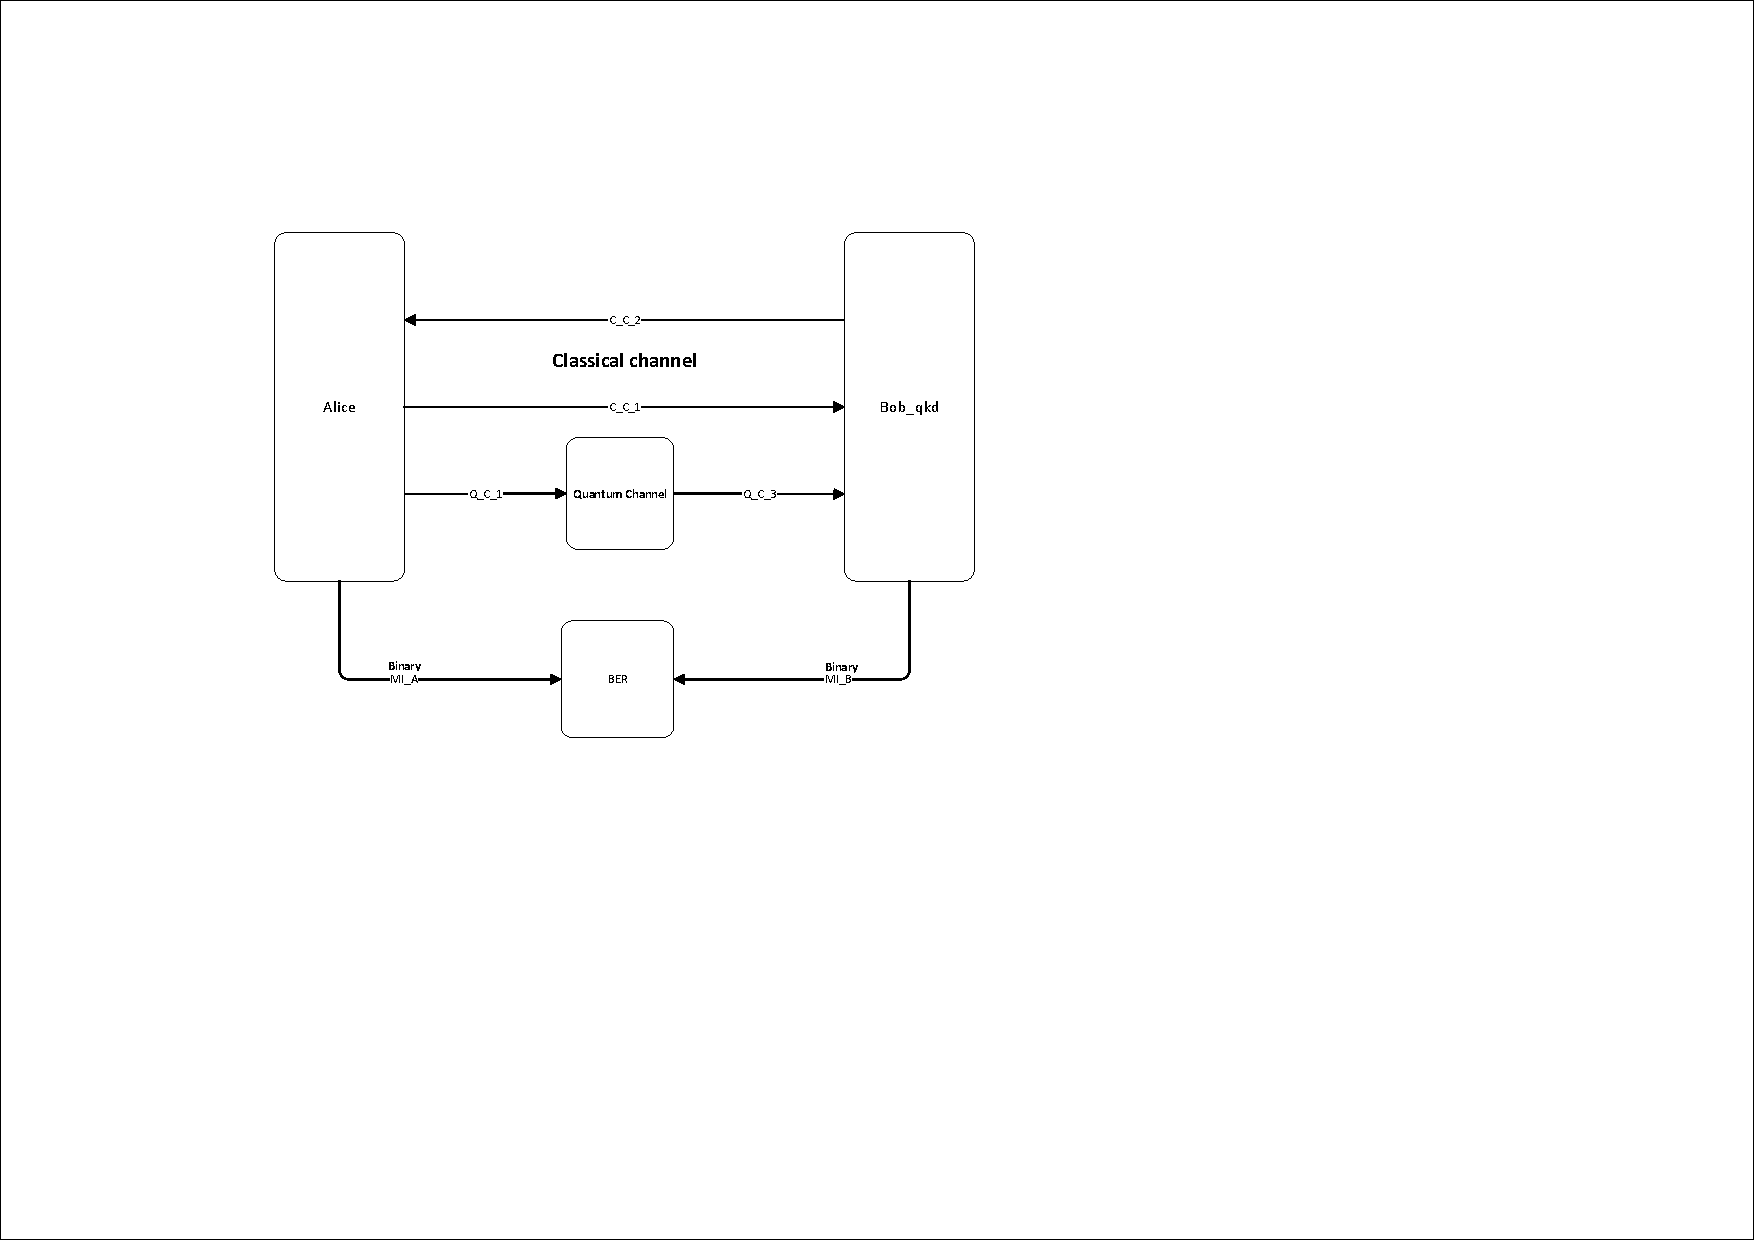
\includegraphics[clip, trim=1cm 8cm 10cm 3cm, width=1.00\textwidth]{./sdf/bb84_with_discrete_variables/figures/Simulation_toplevel_implemented.pdf}
    \caption{Simulation diagram at Alice's side}\label{simulationimplemented}
\end{figure}


Figure \ref{simulationimplemented} presents the top level diagram of our simulation. The setup contains two parties Alice and Bob, where the communication between them is done throughout two authenticated classical channels and one public quantum channel. In a first approach we will perform the simulation without eavesdropper presence. Furthermore, for bit error rate calculation between Alice and Bob.

\begin{figure}[h]
    \centering
        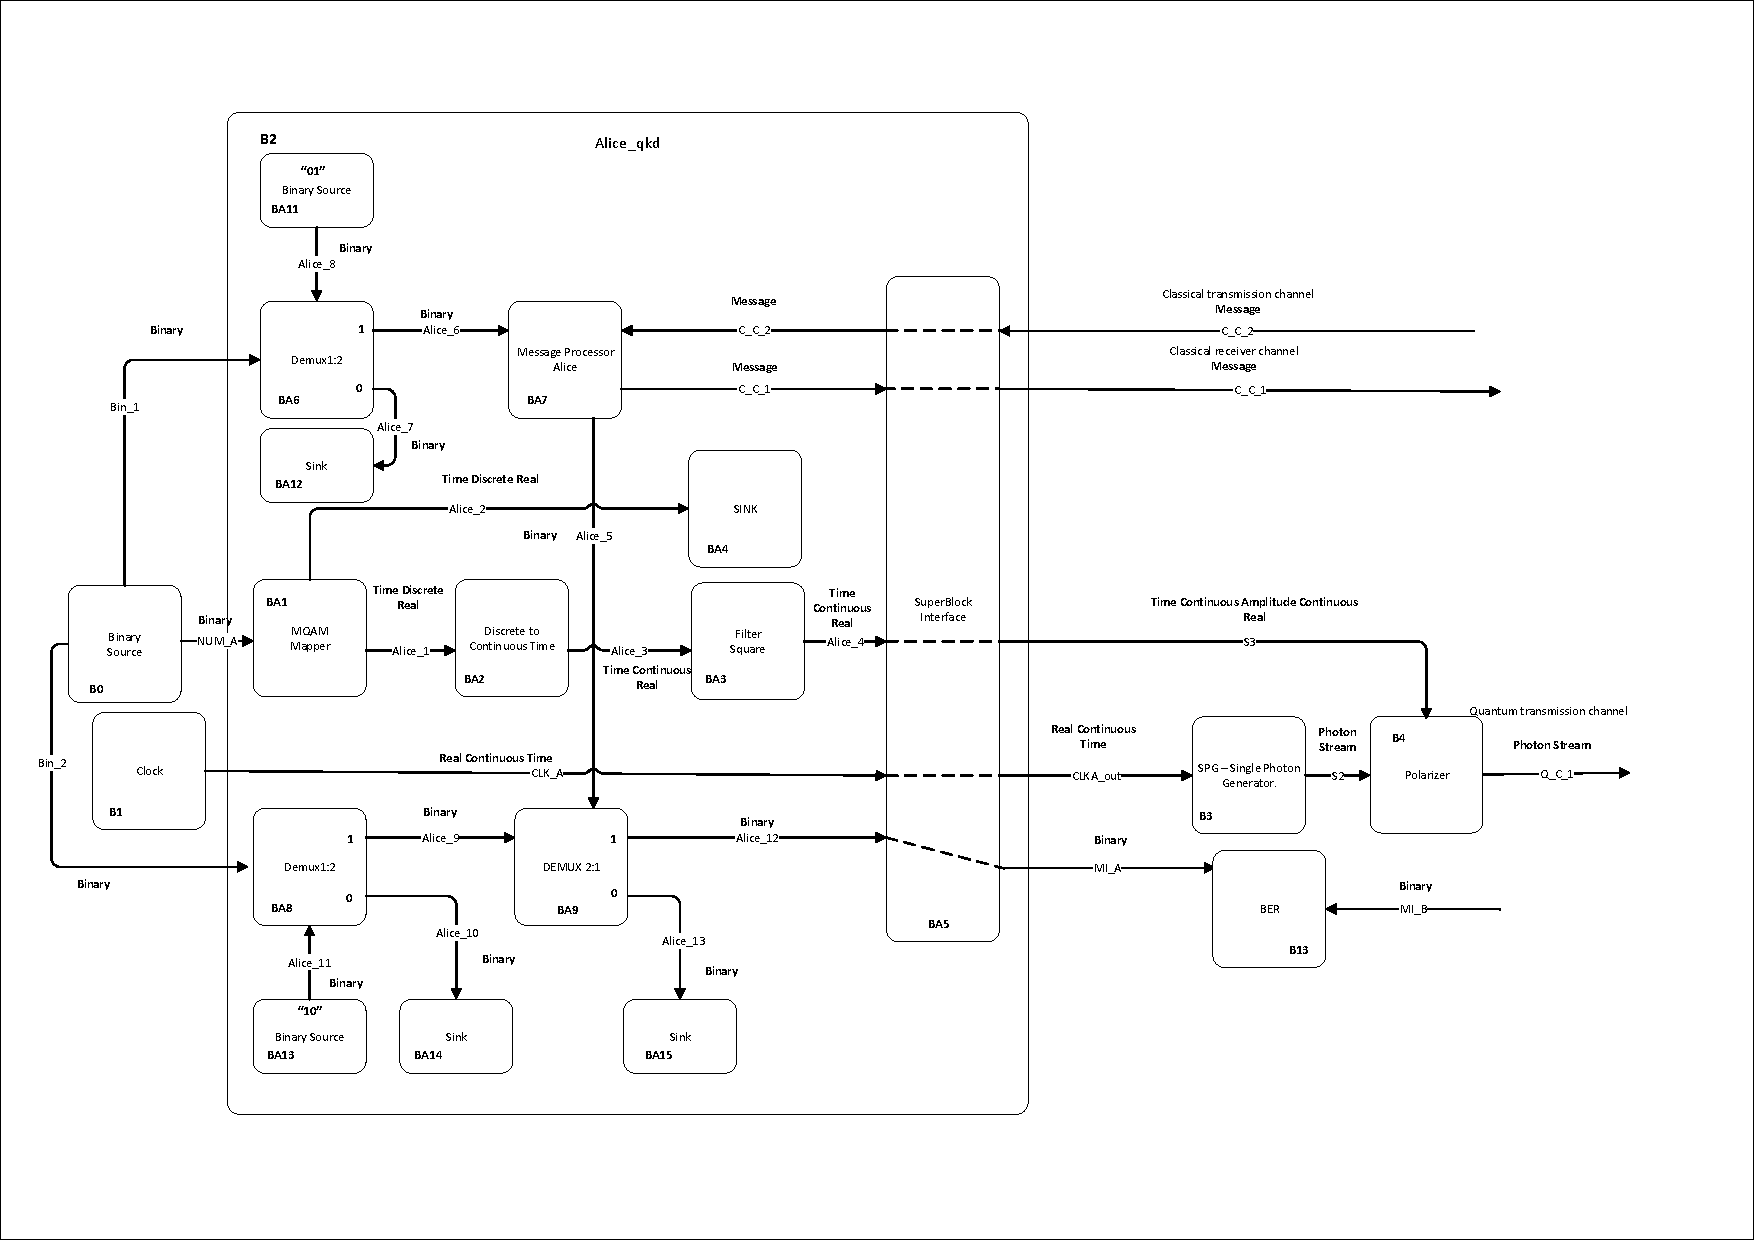
\includegraphics[clip, trim=0.5cm 1cm 0.5cm 1cm, width=1.10\textwidth]{./sdf/bb84_with_discrete_variables/figures/Simulation_Alice_bb84.pdf}
    \caption{Simulation diagram at Alice's side}\label{alicesimulation}
\end{figure}


\begin{figure}[h]
    \centering
        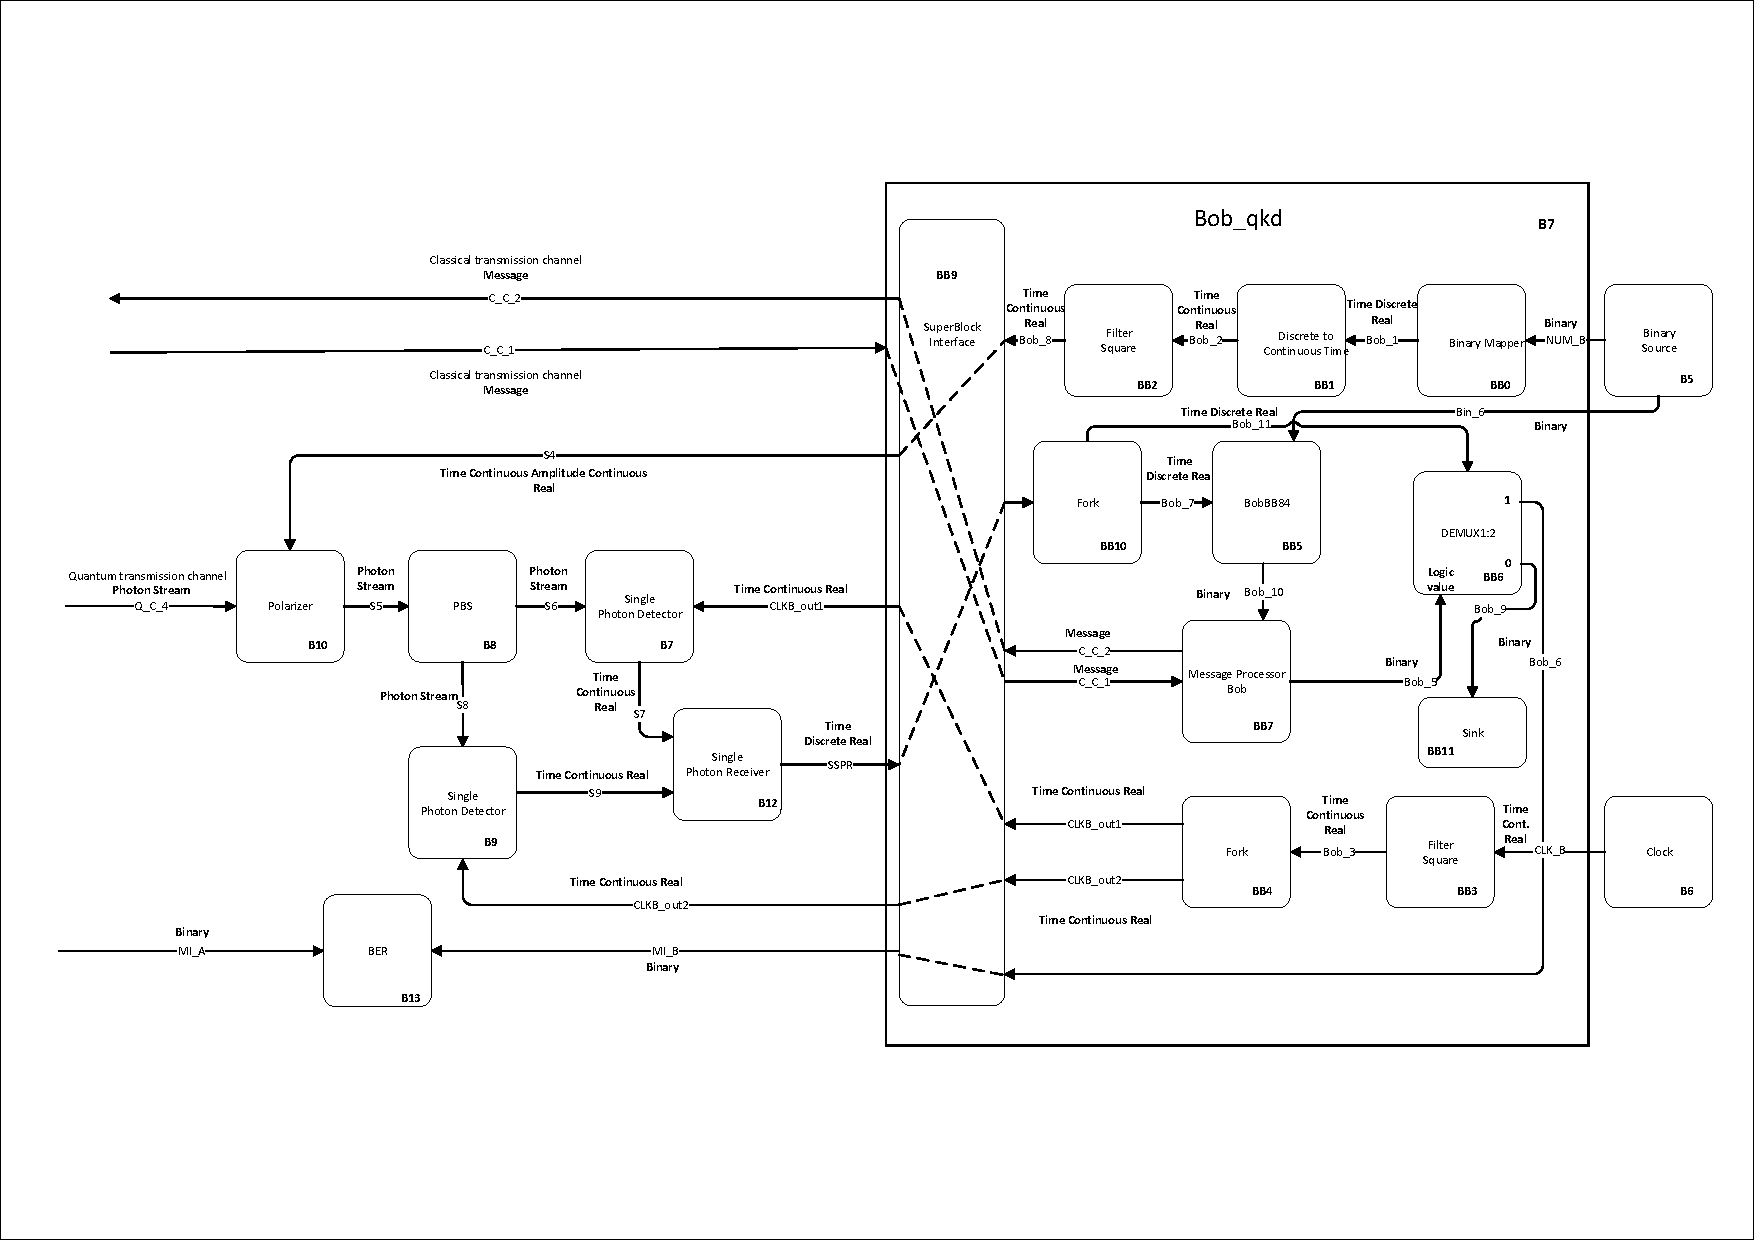
\includegraphics[clip, trim=0.5cm 2.0cm 0.5cm 0.5cm, width=1.00\textwidth]{./sdf/bb84_with_discrete_variables/figures/Simulation_Bob_bb84.pdf}
    \caption{Simulation diagram at Bob's side}\label{bobsimulation}
\end{figure}

    In figure \ref{alicesimulation} one can observe a block diagram of the simulation at Alice's side. As it is shown in the figure, Alice must have one block for random number generation which is responsible for basis generation to polarize the photons, and for key random generation in order to have a random state to encode each photon. Furthermore, she has a Processor block for all logical operations: array analysis, random number generation requests, and others. This block also receives the information from Bob after it has passed through a fork's block. In addition, it is responsible for set the initial length $l$ of the first array of photons which will send to Bob. This block also must be responsible for send classical information to Bob. Finally, Processor block will also send a real continuous time signal to single photon generator, in order to generate photons according to this signal, and finally this block also sends to the polarizer a real discrete signal in order to inform the polarizer which basis it should use. Therefore, she has two more blocks for quantum tasks: the single photon generator and the polarizer block which is responsible to encode the photons generated from the previous block and send them throughout a quantum channel from Alice to Bob.

    Finally, Alice's processor has an output to Mutual Information top level block, $Ms_{A}$.

    In figure \ref{alicesimulation} one can observe a block diagram of the transmitter. As it is shown in the figure, the transmitter must have one block for random number generation (binary source) which is responsible for basis generation to polarize the photons, and for key random generation in order to have a random state to encode each photon. This block has three outputs which will be inputs for the super block Alice. Furthermore, Alice block is responsible for all logical operations: random single photons state values generation, receive and send messages to the receiver Bob by using the classical channels, binary output for mutual information calculations. Each block of the super block is described in Library chapter. Finally, Alice block will also send a real continuous time signal to single photon generator (clock sets the rate oh photons generation), in order to generate photons polarized in the horizontal axis by default. Therefore, the transmitter has one more block, the polarizer block, which is responsible to encode the photons generated from the previous block and send them throughout a quantum channel from Alice to Bob.

     In figure \ref{bobsimulation} one can see a block diagram of the simulation for receiver (Bob). The receiver has one block for Random Number Generation which is responsible for randomly generate basis values which Bob will use to measure the photons sent by Alice throughout the quantum channel. Like transmitter, the receiver has the Bob block responsible for receive and send messages through the classical channel, receive single photons values detection from the single photon detectors, provides a clock signal to the detectors and send binary values for mutual information calculation. Furthermore, the receiver has two blocks for single photon detection (one for horizontal detection and other for vertical detection) which receives from Bob block a real continuous time signal which will set the detection window for the detector and outputs for Bob block the result value for detection. In addition, there is a polarizer which receives from Bob block a time continuous real signal which provides information about the rotation angle. If the basis chosen by Bob is the diagonal basis he sends "$45^\circ$", otherwise sends "$0^\circ$". The polarization beam splitter divides the input photon stream in horizontal component and vertical component.




%\begin{figure}[h]
%	\centering
%	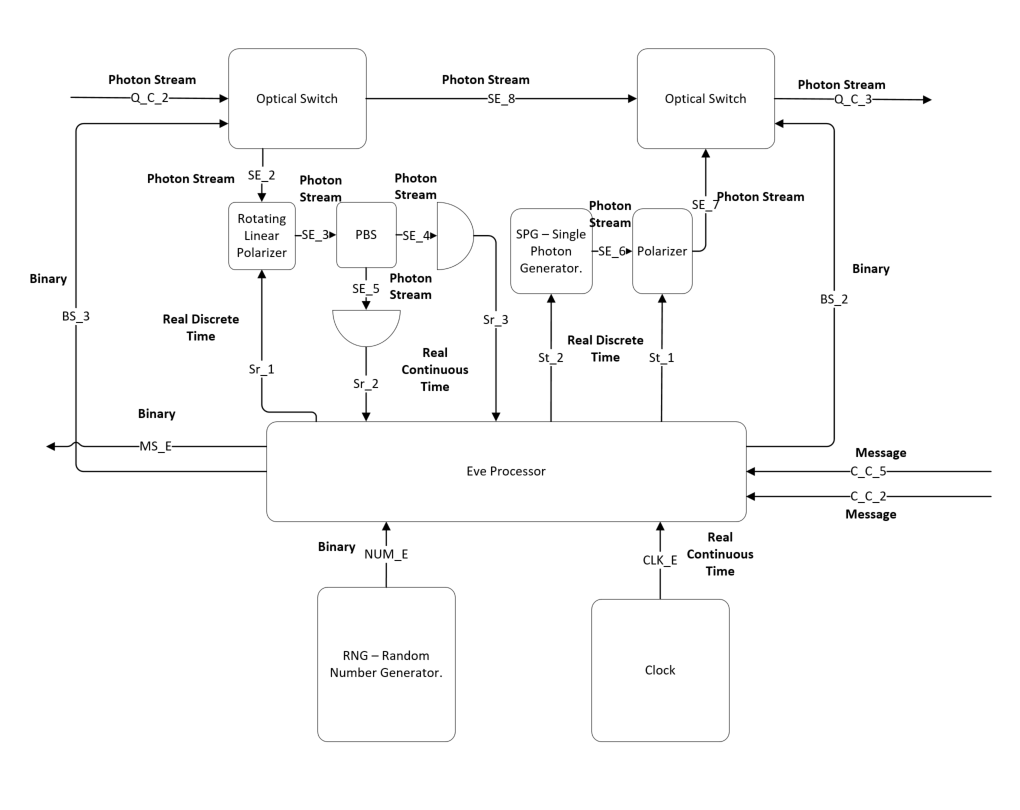
\includegraphics[width=1.1\textwidth, height=14cm]{./sdf/bb84_with_discrete_variables/figures/eve_simulation.png}
%	\caption{Simulation diagram at Eve's side}\label{evesimulation}
%\end{figure}
%
%Figure \ref{evesimulation} presents the Eve's side diagram. Eve's processor has two receiver classical signals, one from Alice (\textbf{C\_C\_2}) and other from Bob (\textbf{C\_C\_5}). About quantum channel, Eve received a quantum message from Alice through the channel \textbf{Q\_C\_1} and depends on her decision the photon can follows directly to Bob or the photon's state can be changed by her. In this case, the photon is received by a block similar to Bob's diagram \ref{bobsimulation} and this block sends a message to Eve's processor in order to reveal the measurement result. After that, Eve's processor sends a message to Alice's diagram similar to figure \ref{alicesimulation} and this block is responsible for encode the photon in a new state. Now, the changed photon is sent to Bob.
%
%In addition, Eve's diagram has one more output $Ms_{E}$ which is a message sent to the mutual information block as an input parameter.

\begin{table}[H]
\centering
\caption{System Signals}
\label{tb:signals}
\begin{tabular}{|c|c|c|}
\hline
\textbf{Signal name}                        & \textbf{Signal type}                      \\ \hline
NUM\_A, NUM\_B, Bin\_1, Bin\_2, Bin\_6      &  Binary                                   \\ \hline
MI\_A, MI\_B                                &  Binary                                   \\ \hline
CLK\_A, CLK\_B                              &  TimeContinuousAmplitudeContinuous        \\ \hline
CLK\_A\_out, CLKB\_out1, CLKB\_out2         &  TimeContinuousAmplitudeContinuous        \\ \hline
S2, S5, S6, S8                              &  PhotonStreamXY                           \\ \hline
S3, S7, S9                                  &  TimeContinuousAmplitudeDiscreteReal      \\ \hline
S4                                          &  TimeContinuousAmplitudeContinuousReal      \\ \hline
C\_C\_1, C\_C\_3                            &  Messages                                 \\ \hline
C\_C\_6, C\_C\_4                            &  Messages                                 \\ \hline
Q\_C\_1, Q\_C\_4                            &  PhotonStreamXY                           \\ \hline

\end{tabular}
\end{table}

Table \ref{tb:signals} presents the system signals as well as them type.

\begin{table}[H]
\centering
\caption{System Input Parameters}
\label{tb:inputparameters}
\begin{tabular}{|c|c|c|}
\hline
\textbf{Parameter}                      & \textbf{Default Value}                                & \textbf{Description} \\ \hline
RateOfPhotons                           & 1K                                                    &                 \\ \hline
iqAmplitudeValues                       & \{-45,0\},\{0,0\},\{45,0\},\{90,0\}   &                 \\ \hline
NumberOfSamplesPerSylbom                & 16                                                    &                   \\ \hline
DetectorWindowTimeOpen                  & 0.2                                                   & smaller than 1 ms \\ \hline
DetectorPulseDelay                      & 0.7                                                   & in units of ms \\ \hline
DetectorProbabilityDarkCount            & 0.0                                                   &    \\ \hline
RotationAngle                           & 0.0                                                   & \\ \hline
ElevationAngle                          & 0.0                                                   & \\ \hline

\end{tabular}
\end{table}

\begin{table}[H]
\centering
\caption{Header Files}
\label{tb:signals}
\begin{tabular}{|c|c|c|}
\hline
\textbf{File name}                                          & \textbf{Description} & \textbf{Status} \\ \hline
netxpto\_20180118.h                                         &                      &    \checkmark      \\ \hline
alice\_qkd\_20180409.h                                      &                      &    \checkmark      \\ \hline
binary\_source\_20180118.h                                  &                      &    \checkmark      \\ \hline
bob\_qkd\_20180409.h                                        &                      &    \checkmark      \\ \hline
clock\_20171219.h                                           &                      &    \checkmark      \\ \hline
discrete\_to\_continuous\_time\_20180118.h                  &                      &    \checkmark      \\ \hline
m\_qam\_mapper\_20180118.h                                  &                      &    \checkmark      \\ \hline
polarization\_beam\_splitter\_20180109.h                    &                      &    \checkmark      \\ \hline
polarization\_rotator\_20180113.h                           &                      &    \checkmark      \\ \hline
pulse\_shaper\_20180111.h                                   &                      &    \checkmark      \\ \hline
single\_photon\_detector\_20180206.h                        &                      &    \checkmark      \\ \hline
single\_photon\_receiver\_20180303.h                        &                      &    \checkmark      \\ \hline
SOP\_modulator\_20180319.h                                  &                      &    \checkmark      \\ \hline
coincidence\_detector\_20180206.h                           &                      &    \checkmark      \\ \hline
single\_photon\_source\_20171218.h                          &                      &    \checkmark      \\ \hline
sink\_20180118.h                                            &                      &    \checkmark      \\ \hline
super\_block\_interface\_20180118.h                         &                      &    \checkmark      \\ \hline
message\_processor\_alice\_20180205.h                       &                      &    \checkmark      \\ \hline
demux\_1\_2\_20180205.h                                     &                      &    \checkmark      \\ \hline
binary\_mapper\_20180205.h                                  &                      &    \checkmark      \\ \hline
bobBB84\_20180221.h                                         &                      &    \checkmark      \\ \hline
message\_processor\_bob\_20180221.h                         &                      &    \checkmark      \\ \hline
sampler\_20171119.h                                         &                      &    \checkmark      \\ \hline
optical\_attenuator\_20180304.h                             &                      &    \checkmark      \\ \hline
fork\_20180112.h                                            &                      &    \checkmark      \\ \hline
\end{tabular}
\end{table}

\begin{table}[H]
\centering
\caption{Source Files}
\label{tb:signals}
\begin{tabular}{|c|c|c|}
\hline
\textbf{File name}                                          & \textbf{Description} & \textbf{Status}    \\ \hline
netxpto\_20180118.cpp                                       &                      &    \checkmark      \\ \hline
bb84\_with\_discrete\_variables\_sdf.cpp                    &                      &    \checkmark      \\ \hline
alice\_qkd\_20180409.cpp                                    &                      &    \checkmark      \\ \hline
binary\_source\_20180118.cpp                                &                      &    \checkmark      \\ \hline
bob\_qkd\_20180409.cpp                                      &                      &    \checkmark      \\ \hline
clock\_20171219.cpp                                         &                      &    \checkmark      \\ \hline
discrete\_to\_continuous\_time\_20180118.cpp                &                      &    \checkmark      \\ \hline
m\_qam\_mapper\_20180118.cpp                                &                      &    \checkmark      \\ \hline
polarization\_beam\_splitter\_20180109.cpp                  &                      &    \checkmark      \\ \hline
polarization\_rotator\_20180113.cpp                         &                      &    \checkmark      \\ \hline
pulse\_shaper\_20180111.cpp                                 &                      &    \checkmark      \\ \hline
single\_photon\_detector\_20180206.cpp                      &                      &    \checkmark      \\ \hline
single\_photon\_receiver\_20180303.cpp                      &                      &    \checkmark      \\ \hline
SOP\_modulator\_20180319.cpp                                &                      &    \checkmark      \\ \hline
coincidence\_detector\_20180206.cpp                         &                      &    \checkmark      \\ \hline
single\_photon\_source\_20171218.cpp                        &                      &    \checkmark      \\ \hline
sink\_20180118.cpp                                          &                      &    \checkmark      \\ \hline
super\_block\_interface\_20180118.cpp                       &                      &    \checkmark      \\ \hline
message\_processor\_alice\_20180205.cpp                     &                      &    \checkmark      \\ \hline
demux\_1\_2\_20180205.cpp                                   &                      &    \checkmark      \\ \hline
binary\_mapper\_20180205.cpp                                &                      &    \checkmark      \\ \hline
bobBB84\_20180221.cpp                                       &                      &    \checkmark      \\ \hline
message\_processor\_bob\_20180221.cpp                       &                      &    \checkmark      \\ \hline
sampler\_20171119.cpp                                       &                      &    \checkmark      \\ \hline
optical\_attenuator\_20180304.cpp                           &                      &    \checkmark      \\ \hline
fork\_20180112.cpp                                          &                      &    \checkmark      \\ \hline
\end{tabular}
\end{table}

\subsubsection{Simulation Results}

Figure \ref{toplevelalicebob} represents the block diagram of the first simulation performed between Alice and Bob. This simulation intends to simulate the communication protocol between Alice and Bob until they do the Basis Reconciliation. At this time, it is not taken into account any attack from an eavesdropper. However, as one can learn from theoretical protocol analysis, the attenuation due the fiber losses, dark counts probabilities from single photon detectors and the SOP drift over the quantum channel are all taken into account.

\begin{figure}[h]
    \centering
        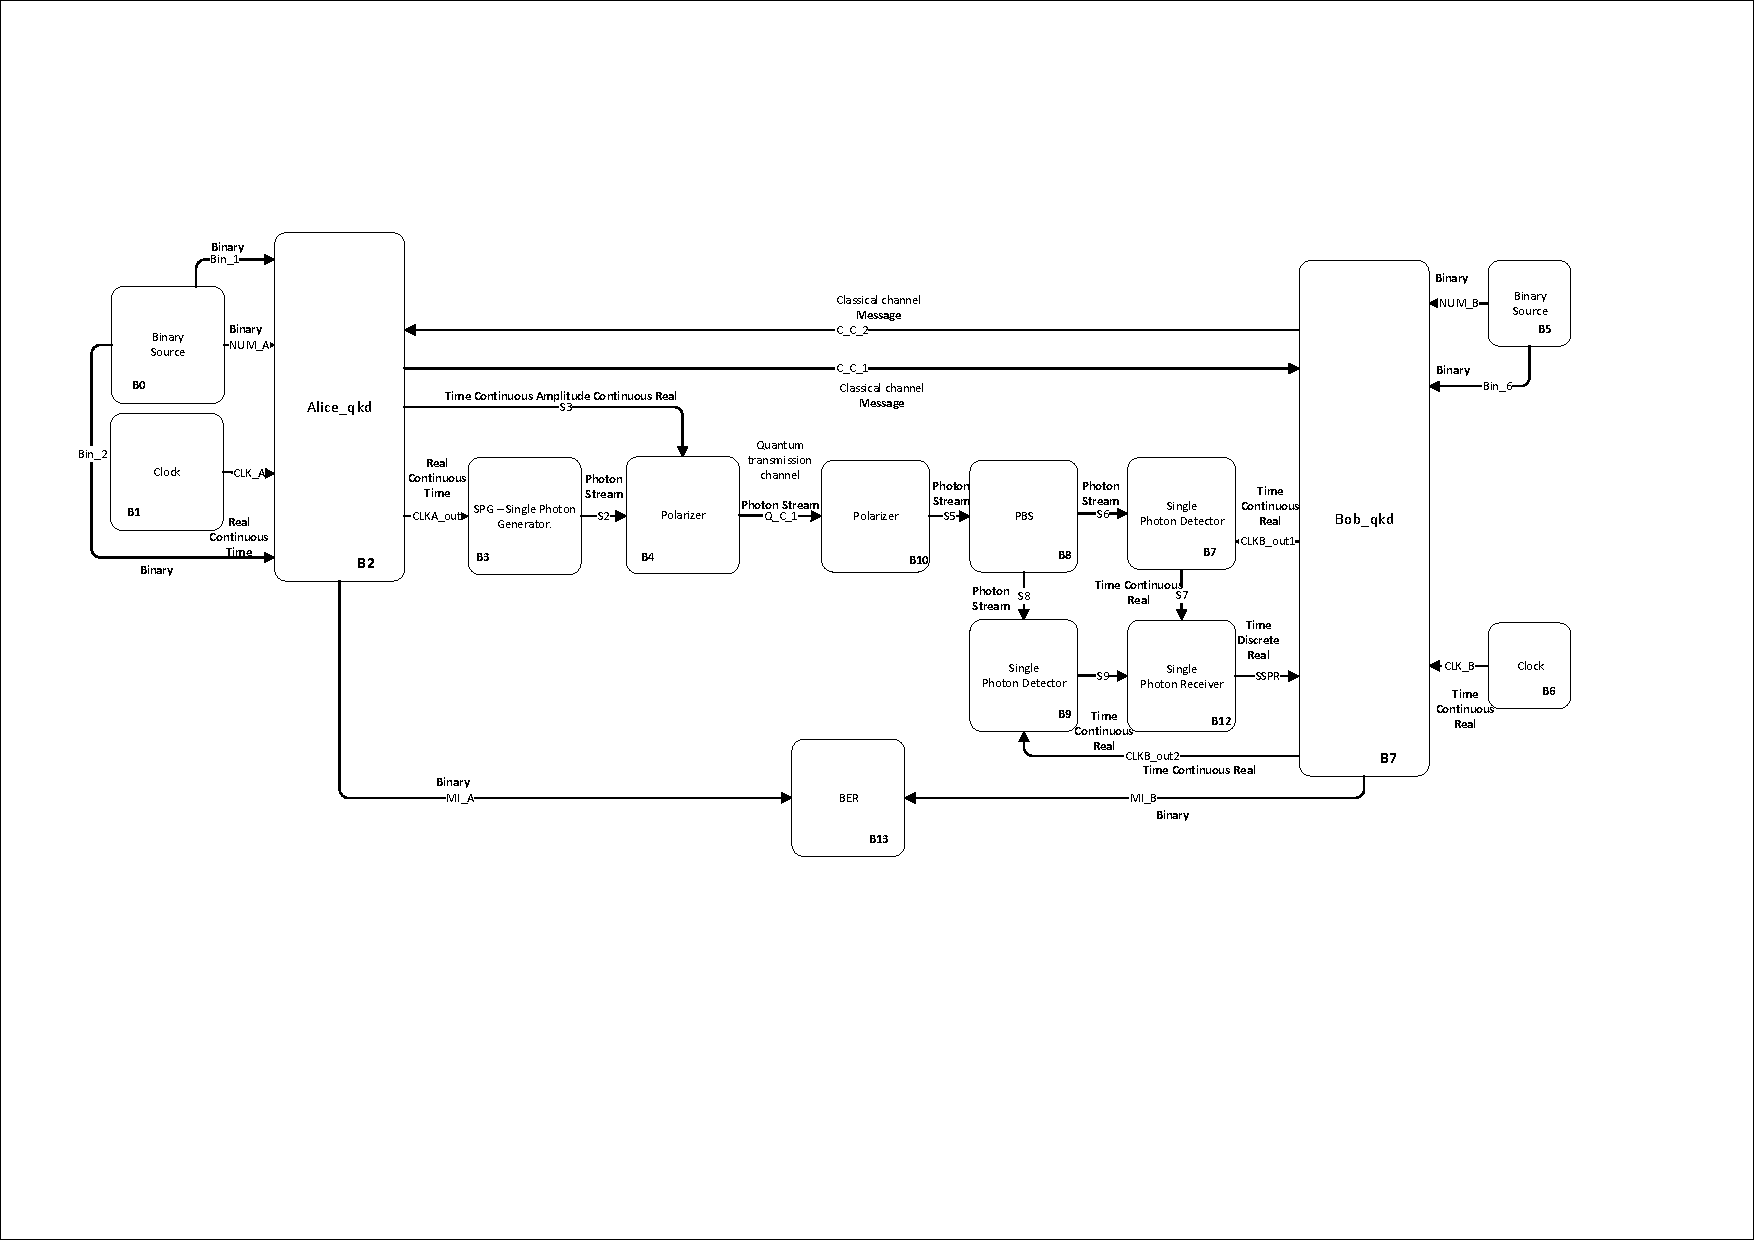
\includegraphics[clip=true, trim=1.2cm 5.0cm 0.5cm 2.5cm, width=1.10\textwidth]{./sdf/bb84_with_discrete_variables/figures/Simulation_toplevel_bb84.pdf}
    \caption{Diagram block of simulation performed between Alice and Bob until Basis Reconciliation. }\label{toplevelalicebob}
\end{figure}

Alice starts by sending a sequence of photons to Bob, and then he measures the photons according to random basis randomly generated by his binary source. After that, he follows the protocol described above until Alice sends to him a string of '0' and '1' where '0' means that both used different basis and '1' means that they used the same basis. Therefore, Alice and Bob outputs a binary signal "MI\_A" and "MI\_B", respectively. In case of no errors occurred in the quantum channel, these signals should be equal in order to both have the same sequence of bits. Furthermore, QBER between the two sequences should be $0$. This way, Alice can encode messages using these keys and Bob will be capable of decrypt the message using these symmetric keys. When errors are introduced in quantum channel QBER value will increase as we can see later.

\begin{figure}[H]
    \centering
        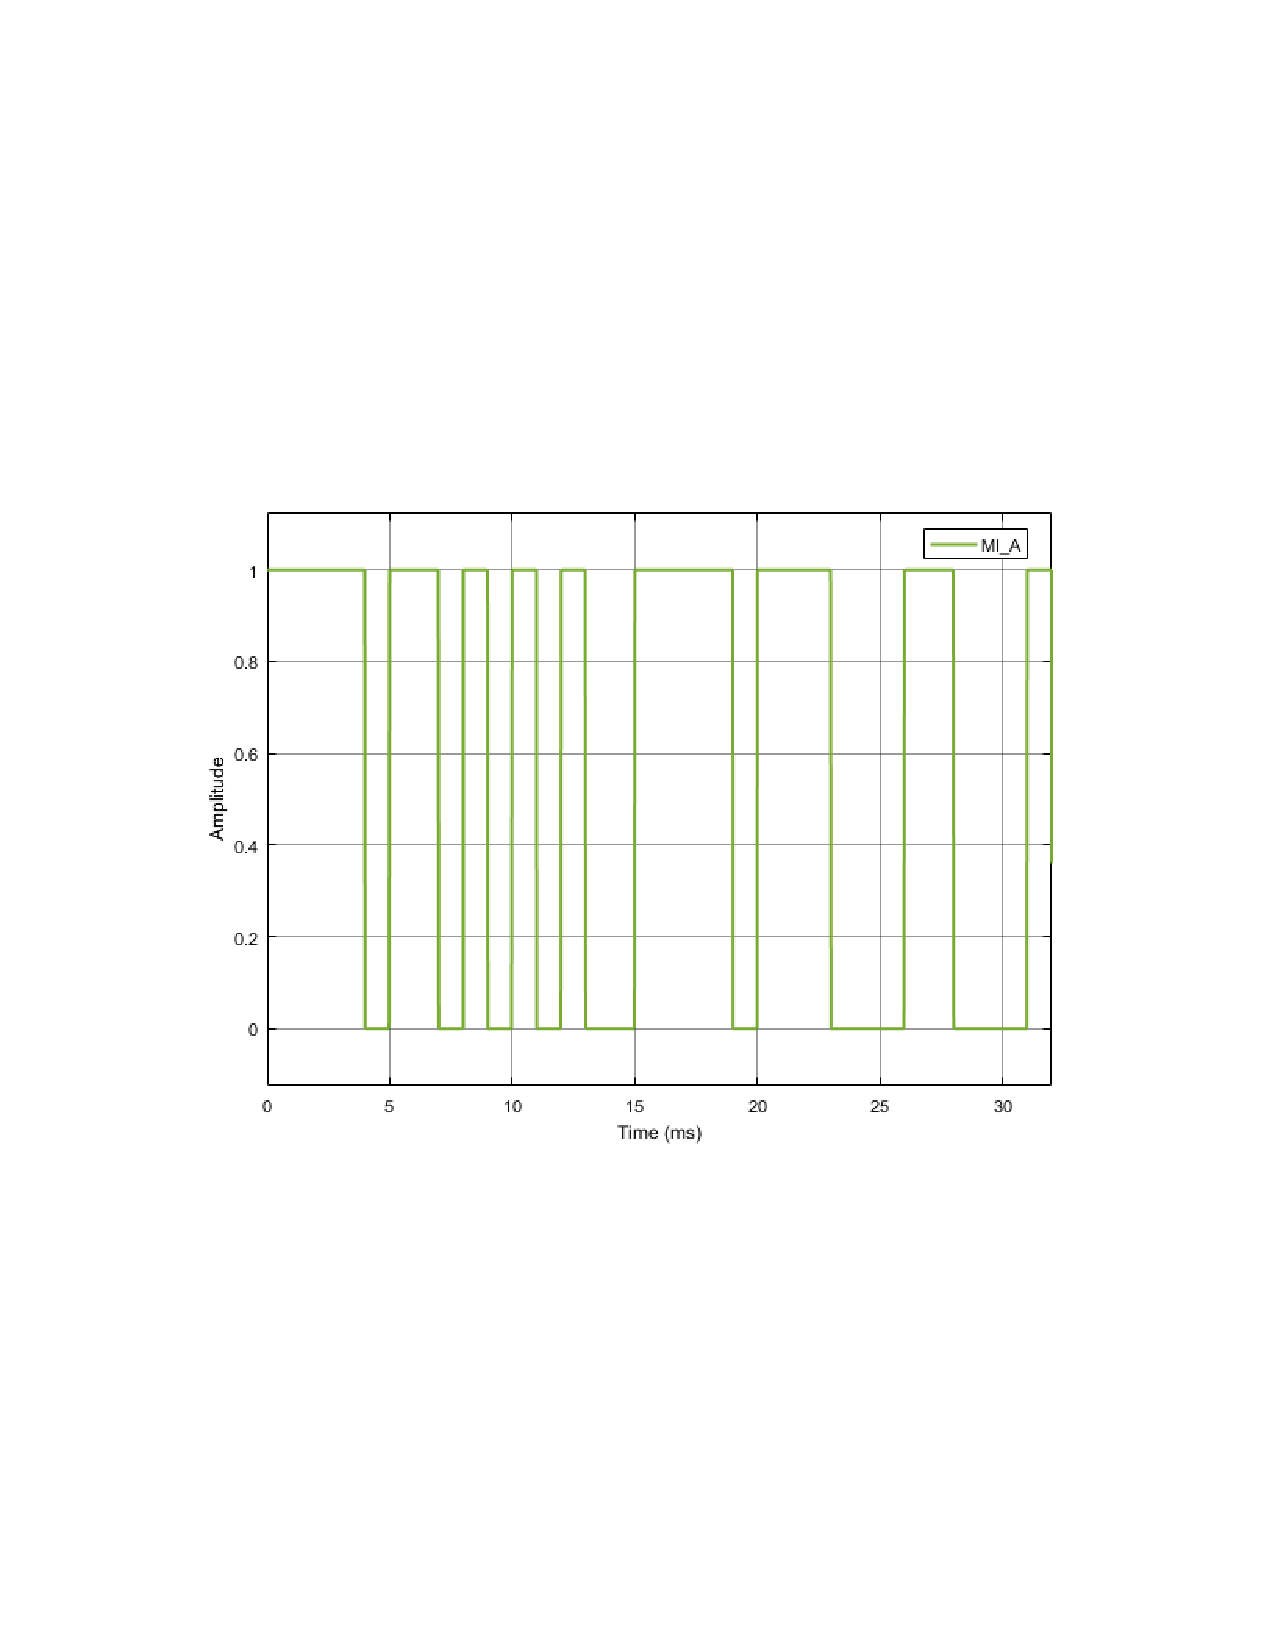
\includegraphics[clip, trim=3cm 9.0cm 2cm 7cm, width=0.50\textwidth]{./sdf/bb84_with_discrete_variables/figures/mia.pdf}
    \caption{MI\_A signal. }\label{mia}
\end{figure}

Figure \ref{mia} and figure \ref{mib} represent the sequence of bits which will be used by Alice to encode the messages and the sequence of bits used by Bob to decode the message when no errors in quantum channel are taken into account, respectively. As one can see the two signals are equal which meets the expected result. In this way, the first step of the protocol has been achieved.

\begin{figure}[h]
    \centering
        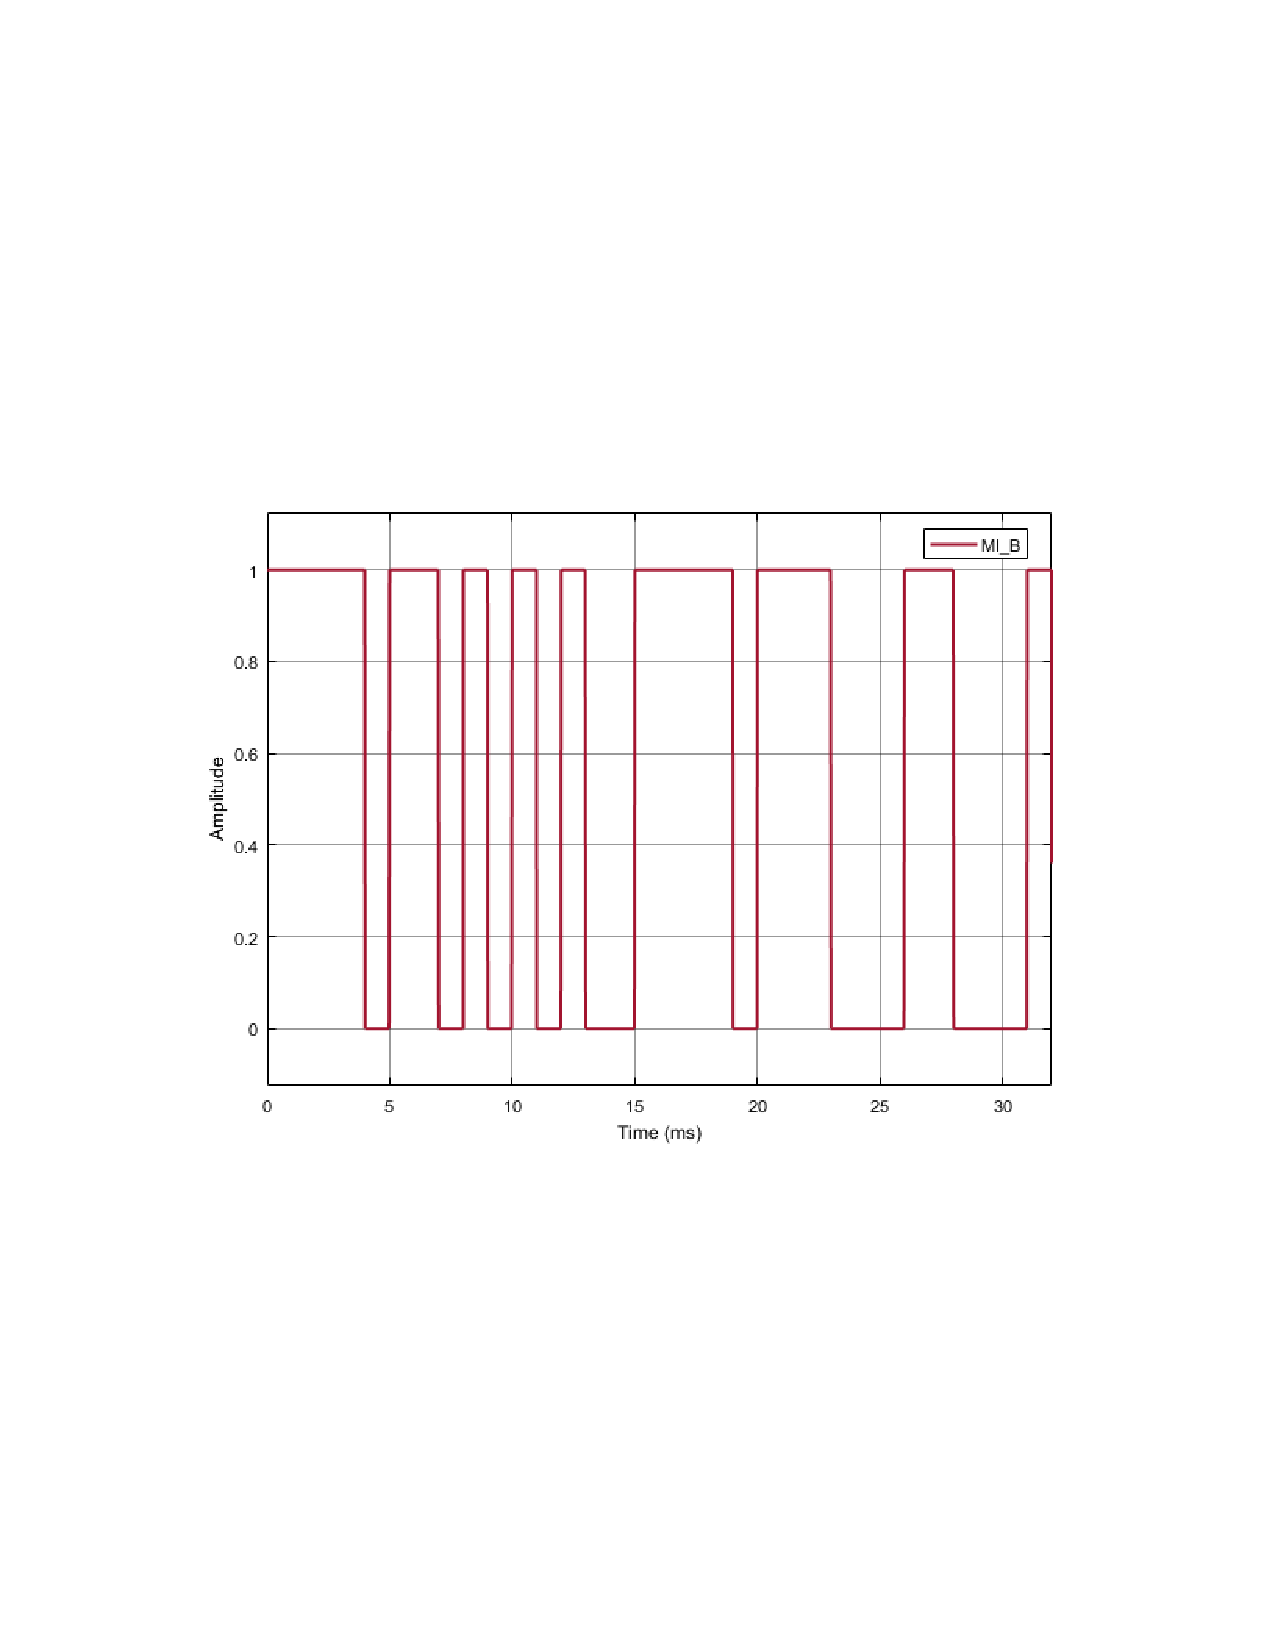
\includegraphics[clip, trim=3cm 9.5cm 2cm 7cm, width=0.50\textwidth]{./sdf/bb84_with_discrete_variables/figures/mib.pdf}
    \caption{MI\_B signal. }\label{mib}
\end{figure}

As one can see in figure \ref{toplevelsimulation} a block which calculates QBER is connected to Alice and Bob. This block calculates the QBER between the measurements that Bob performed with the same basis as Alice, based on method described in \cite{Muga11}. Thus, as expected, the QBER is $0 \%$ when no errors are taken into account.

Next, some errors due the changes in state of polarization of the single photons transmitted between Alice and Bob were added. This way, a polarization rotator in the middle of the quantum channel was added, which is controlled by a SOP modulator block as it is shown in figure \ref{sop_channel} with modelled with deterministic \cite{Muga15} and stochastic \cite{Czegledi16} methods. Additional information about the blocks presented in this quantum channel can be found in library chapter.

\begin{figure}[h]
    \centering
        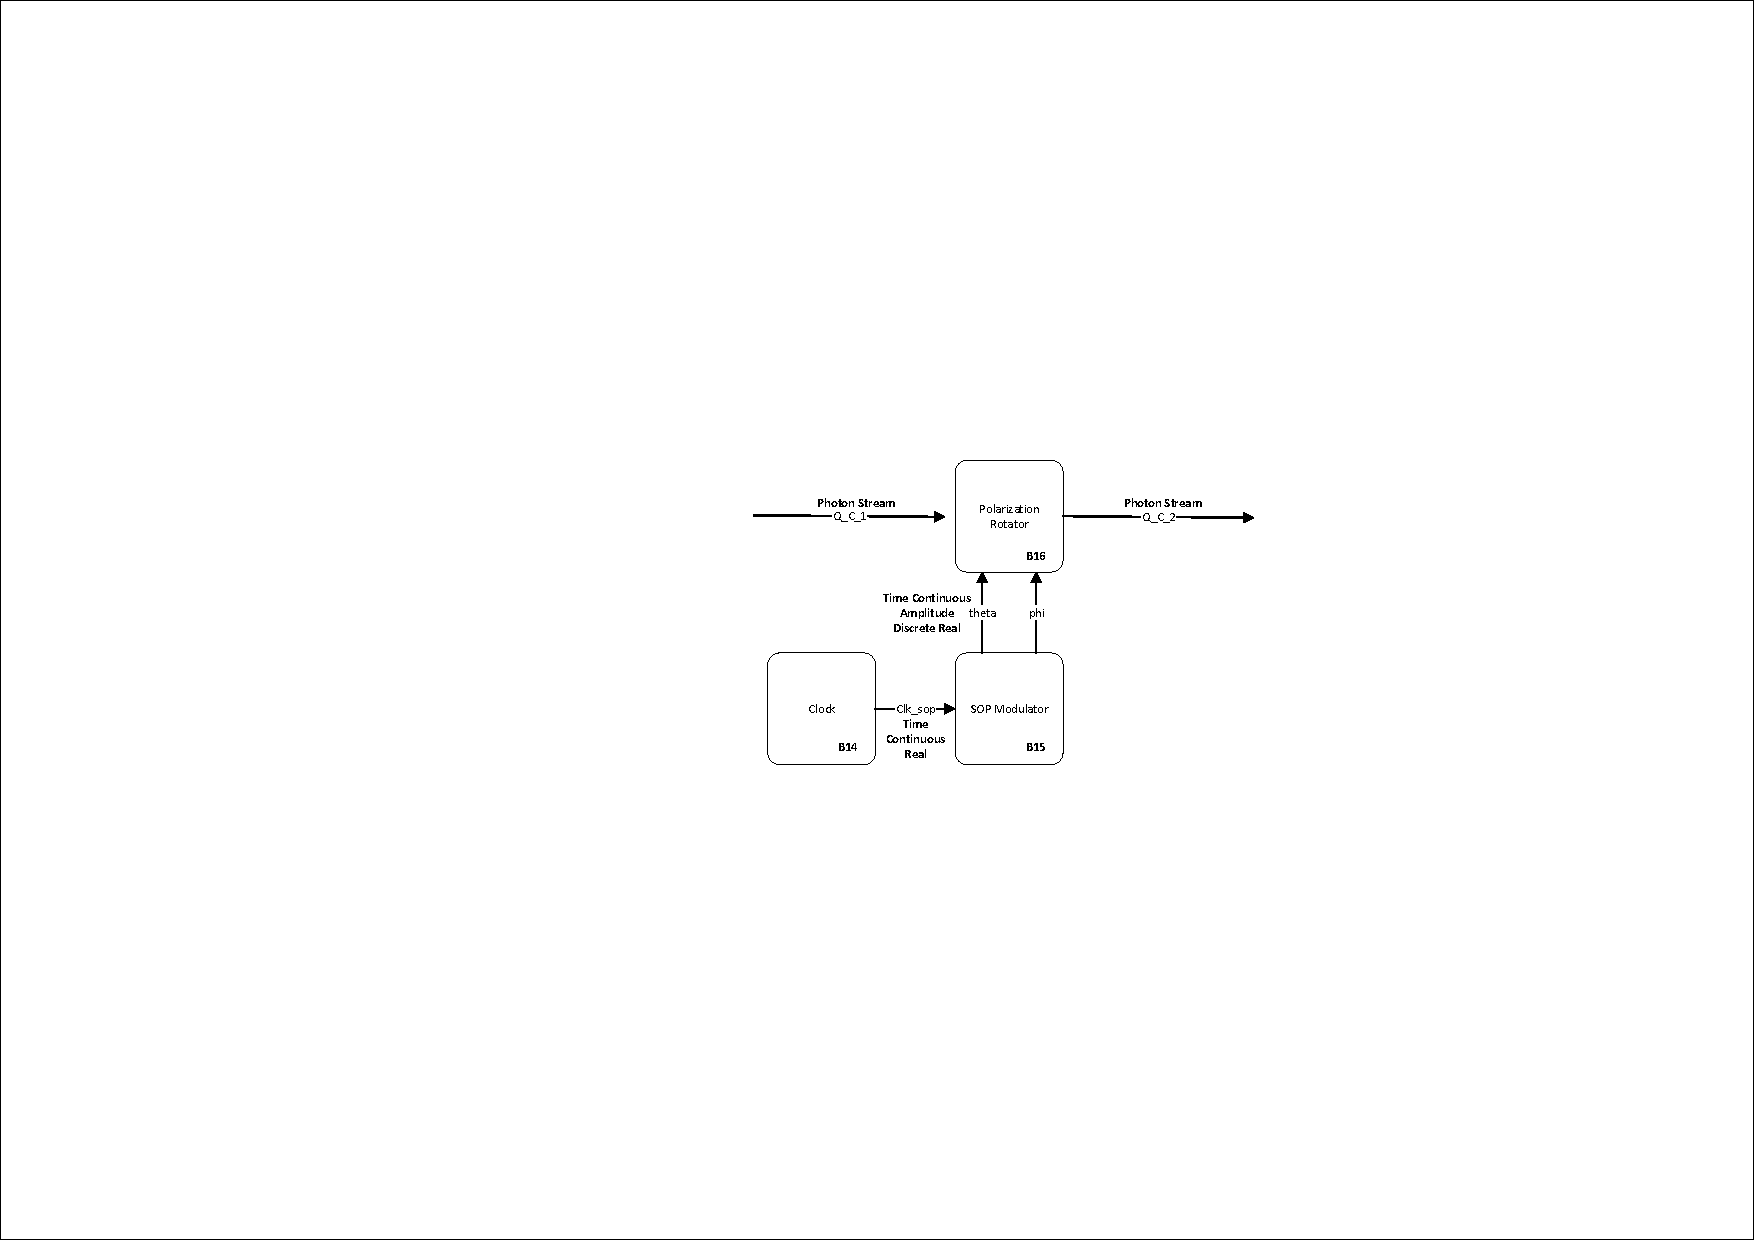
\includegraphics[clip, trim=9cm 7.0cm 5cm 7.5cm, width=0.80\textwidth]{./sdf/bb84_with_discrete_variables/figures/Simulation_sop.pdf}
    \caption{Quantum channel diagram. }\label{sop_channel}
\end{figure}

Now, it is important to calculate the QBER as a function of the rotation angle $\theta$. In order to do that, it was simulated a deterministic SOP modulation, in which the $\theta$ angle varies over the time. In figure \ref{qber} is presented the variation in the value of QBER with respect with theta changes from $0^\circ$ to $45^\circ$. Theoretically, QBER corresponds to the probability of errors in the channel. Which means that in practice this probability corresponds to the probability of a photon following the wrong path in the polarization beam splitter immediately before the detection circuit.

\begin{figure}[h]
    \centering
        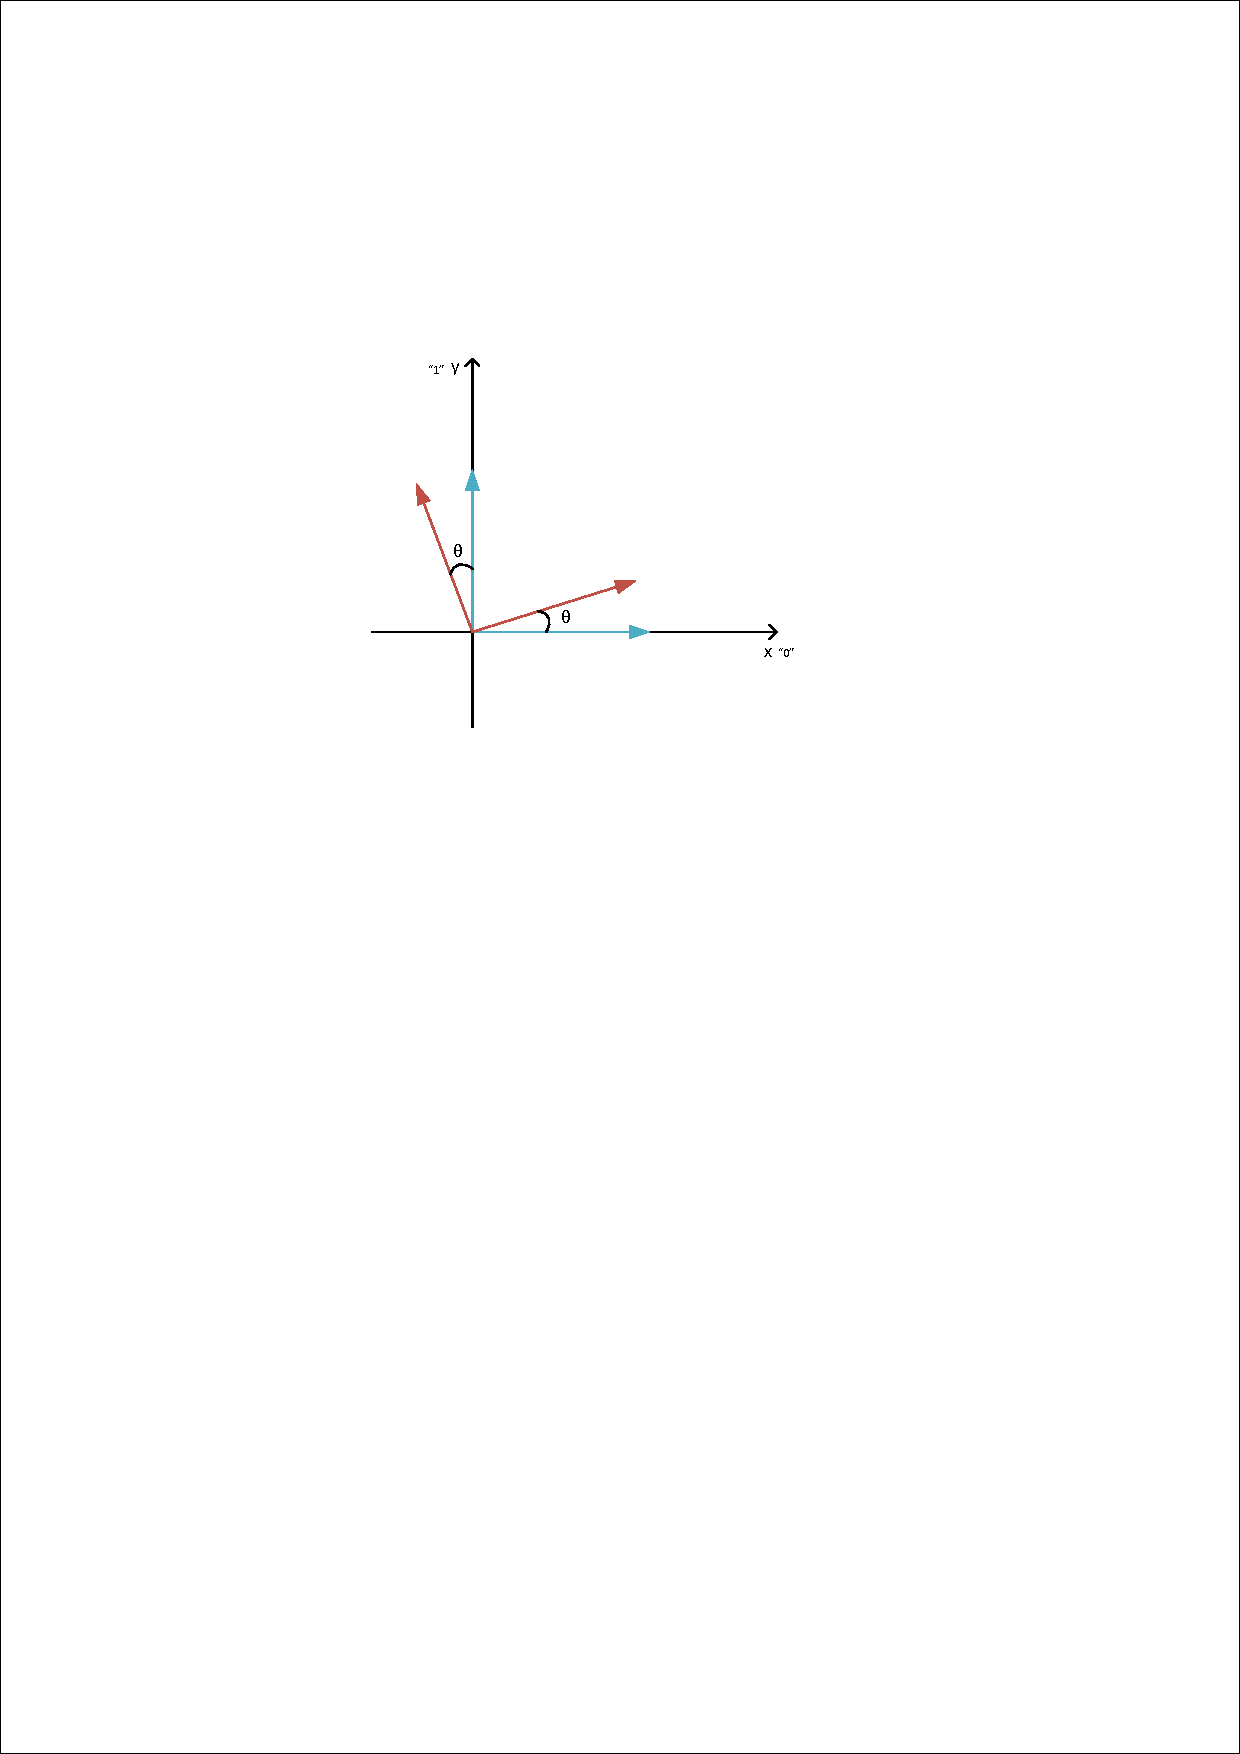
\includegraphics[clip, trim=4cm 17.0cm 5cm 17cm, width=0.80\textwidth]{./sdf/bb84_with_discrete_variables/figures/prob_qber.pdf}
    \caption{Representation of two orthogonal states rotated by an angle $\theta$.}\label{rep_rotation}
\end{figure}

Figure \ref{rep_rotation} presents the graphical representation of two orthogonal states rotated by an angle $\theta$. This rotation is induced by the SOP modulator block which selects a deterministic $\theta$ and $\phi$ angles that do not change over the time. This same rotation is applied for all sequential samples. From figure \ref{rep_rotation} the theoretical QBER can be calculated using the following equation:

\begin{equation}\label{eq:qber}
  QBER = P(0)P(1|0)+P(1)P(0|1).
\end{equation}

Since we have been using a polarization beam splitter 50:50,

\begin{equation*}
  P(0) = P(1) = \frac{1}{2}.
\end{equation*}

This way,
\begin{eqnarray}\label{eq:qber_final}
% \nonumber % Remove numbering (before each equation)
   QBER & = & \frac{1}{2}sin^2(\theta)+ \frac{1}{2}sin^2(\theta)\\
   QBER & = & sin^2(\theta).
\end{eqnarray}

 In figure \ref{qber} are represented two curves: qber calculated from simulated data and qber calculated using theoretical model from equation \ref{eq:qber_final}. Furthermore, the cross correlation coefficient between the two signals was calculated using a function from MATLAB \textit{xcorr(x,y,'coeff')} which the result is $99.92\%$. From that, we can conclude that the QBER calculated from simulated data follows the theoretical curve with high correlation. Nevertheless, the error bars presented in figure \ref{qber} were calculated based on a confidence interval of $95\%$.

\begin{figure}[h]
    \centering
        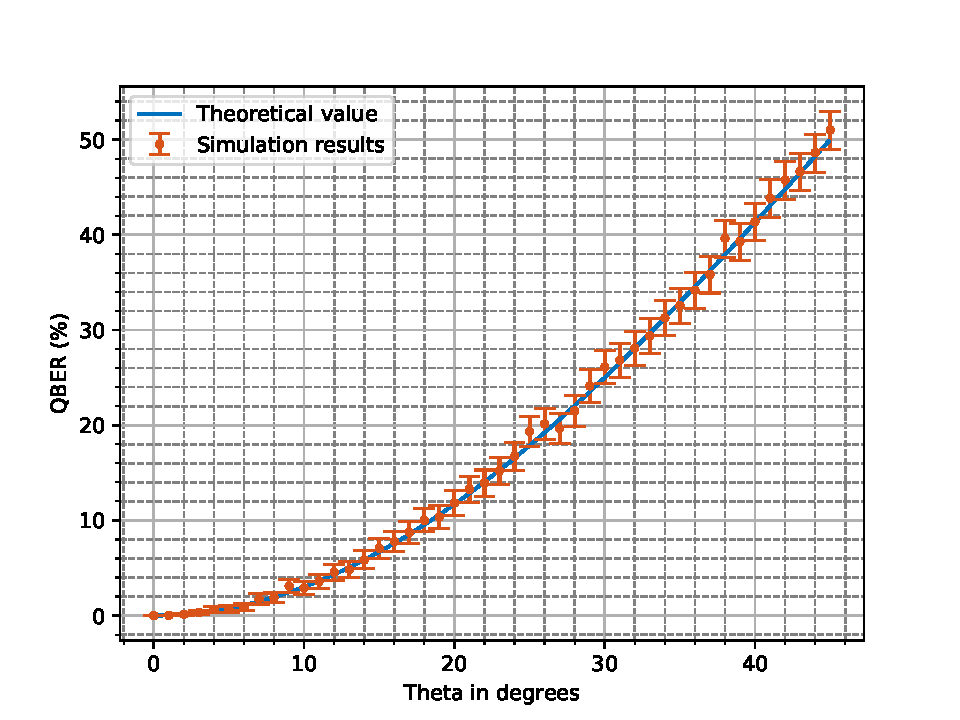
\includegraphics[clip, trim=0.5cm 0.0cm 0.5cm 1cm, width=0.80\textwidth]{./sdf/bb84_with_discrete_variables/figures/QBER_vs_theta_normal_scale.pdf}
    \caption{Qber evolution in relation with deterministic SOP drift.}\label{qber}
\end{figure}

\begin{figure}[H]
    \centering
        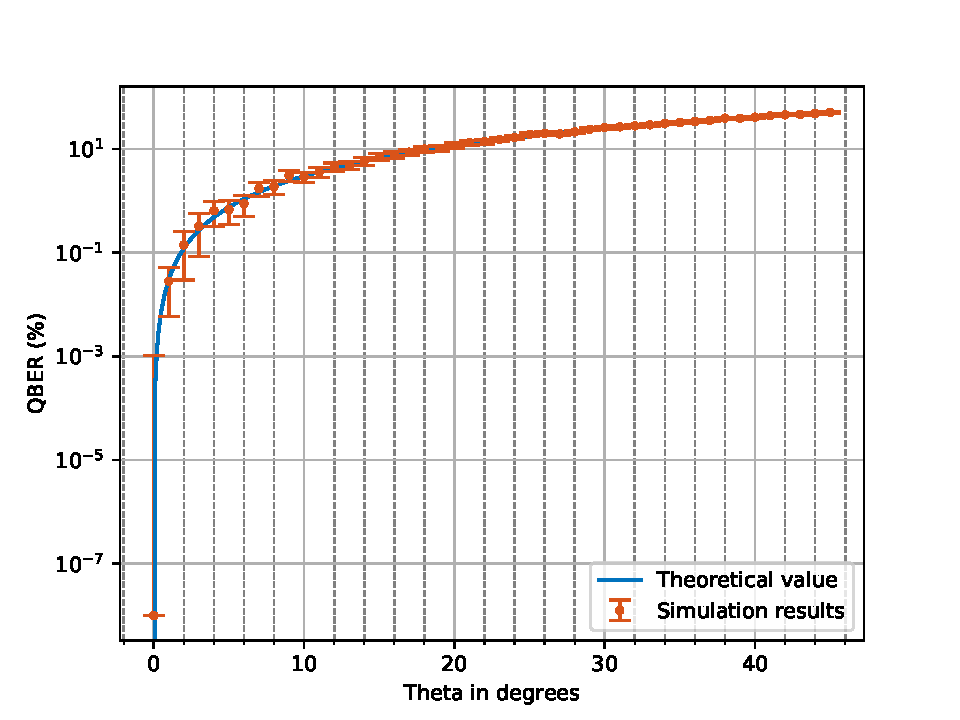
\includegraphics[clip, trim=0.2cm 0.0cm 0.5cm 1cm, width=0.80\textwidth]{./sdf/bb84_with_discrete_variables/figures/qber_vs_theta_all.pdf}
    \caption{Qber evolution in relation with deterministic SOP drift in log scale.}\label{qber_log}
\end{figure}

\begin{figure}[H]
    \centering
        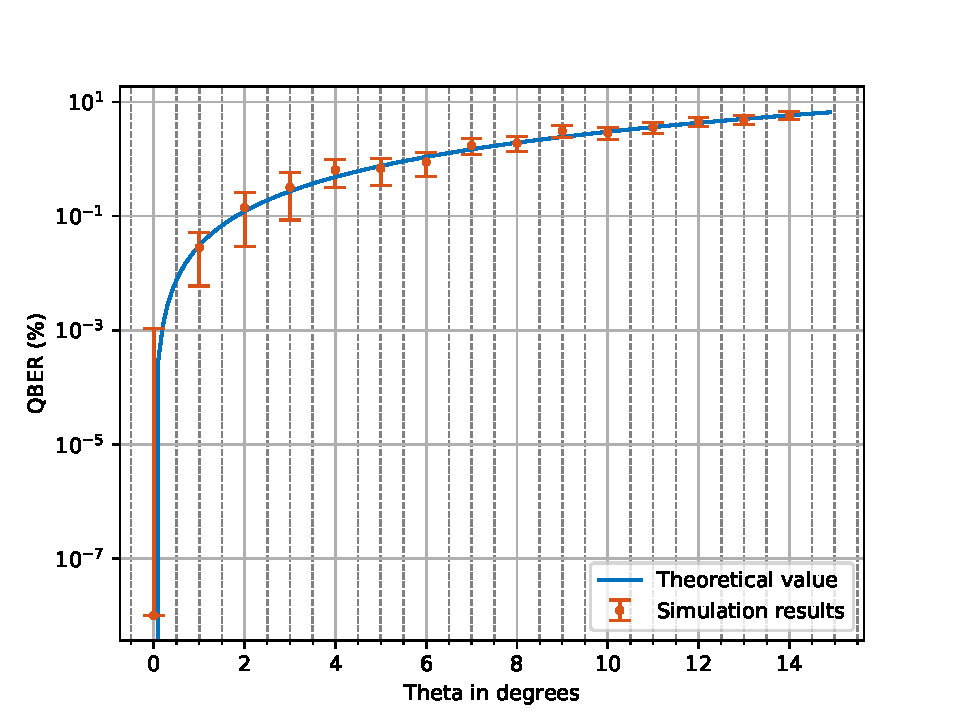
\includegraphics[clip, trim=0.2cm 0.0cm 0.5cm 1cm, width=0.80\textwidth]{./sdf/bb84_with_discrete_variables/figures/QBER_vs_theta_upto15.pdf}
    \caption{Qber evolution in relation with deterministic SOP drift scaled.}\label{qber_log_scaled}
\end{figure}
\newpage

\subsection{Open Issues}
\begin{enumerate}
   
    \item Implementation of the scrambling algorithm in order to spread the errors.
    \item Implementation of the control system for polarization rotations.
    \item Implementation of a QBER estimation protocol.
    \item Implementation of the cascade for error correction.
    \item Implementation of the output which represents the final key that is built.
    \item Introduce EVE in simulation as shown in figure \ref{toplevelsimulation2}.
        \begin{figure}[H]
        	\centering
        	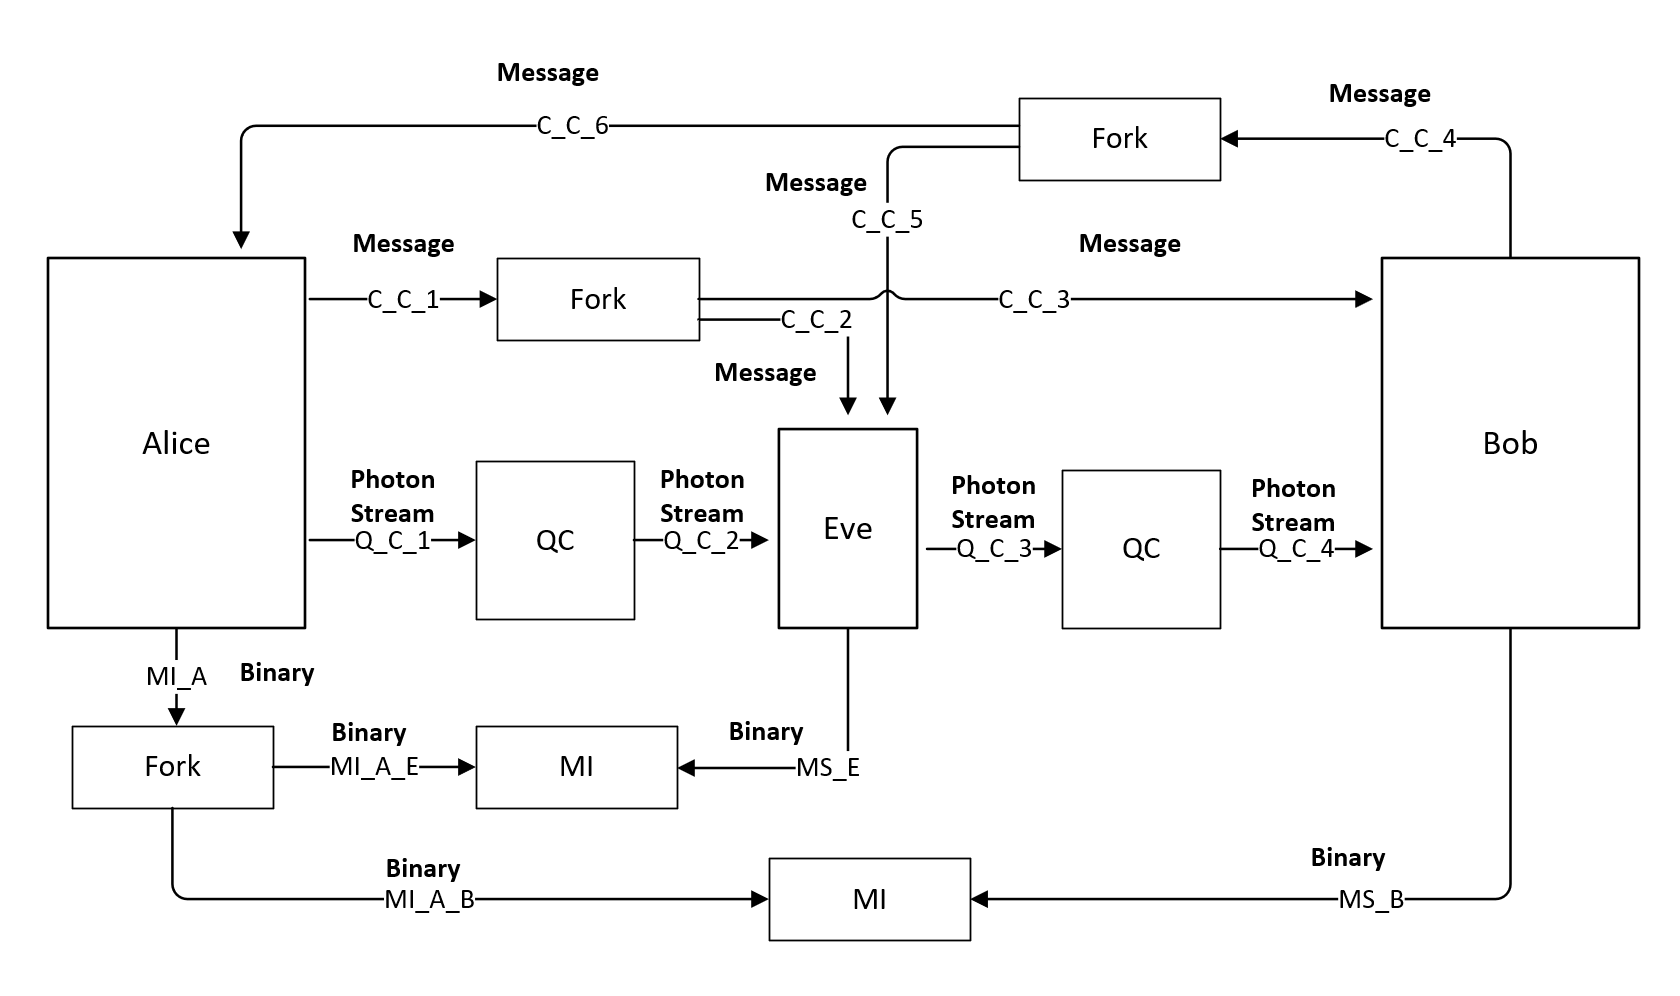
\includegraphics[width=1.0\textwidth, height=9cm]{./sdf/bb84_with_discrete_variables/figures/toplevel_simulation.png}
        	\caption{Simulation diagram at a top level}\label{toplevelsimulation2}
        \end{figure}
    \item Experimental Implementation.
\end{enumerate}
  


\newpage


% COLOCAR ESTAS REFERÊNCIAS NUM FICHEIRO BIB
%
%\begin{thebibliography}{2}
%	\bibitem{BB84}
%	Bennett, C. H. and Brassard,
%	G. Quantum Cryptography: Public key distribution and coin tossing.
%	International Conference on Computers, Systems and Signal Processing, Bangalore, India, 10-12 December 1984, pp. 175-179.
%	
%	\bibitem{SURV}
%	Mart Haitjema, A Survey of the Prominent Quantum Key Distribution Protocols
%	
%	\bibitem{iqo}
%	Christopher Gerry, Peter Knight, "Introductory Quantum Optics" Cambridge University Press, 2005
%	
%	\bibitem{SPREADING}
%	Varadarajan, S., Ngo, H. Q., \& Srivastava, J. (n.d.). An Adaptive , Perception-Driven Error Spreading Scheme in Continuous Media Streaming.
%	
%\end{thebibliography}

% bibliographic references for the section ----------------------------
\clearpage
\printbibliography[heading=subbibliography]
\end{refsection}
\addcontentsline{toc}{subsection}{Bibliography}
\cleardoublepage
% ---------------------------------------------------------------------  \fi
\ifdefined\qokd         \input{./sdf/qokd_with_discrete_variables/qokd_with_discrete_variables} \fi
\ifdefined\quantumA     \input{./sdf/quantum_noise/quantum_noise} \fi
\ifdefined\cvQuantum    \input{./sdf/cv_system/cv_system} \fi
\ifdefined\intradyne    \input{./sdf/intradyne_cv_system/intradyne_cv_system} \fi
\ifdefined\classicalMpc \section{Classical Multi-Party Computation}

\begin{refsection}

\subsection{Introduction}
Multi-Party Computation (MPC), also known as Secure Function Evaluation, allows two or more parties
to correctly compute a function of their private inputs without exposure, i.e., without
the input of one party being revealed to the other parties.
In other terms, a generic function \textit{f} receives as input a set $\{a_1,a_2,\dots,a_n\}$
of arguments, where $a_i$ is the input of the i-th party, and $1\leq i\leq n$, and outputs a value \textit{c}, which represents the result
of the joint computation of \textit{f}, as shown in Figure \ref{fig:mpcscheme}.
The output of \textit{f} is given by the following expression.
\begin{equation}\label{eq:mpc}
c = f(a_1,a_2,\dots,a_n)
\end{equation}

\renewcommand{\figurename}{Figure}
\begin{figure}[H]
\centering
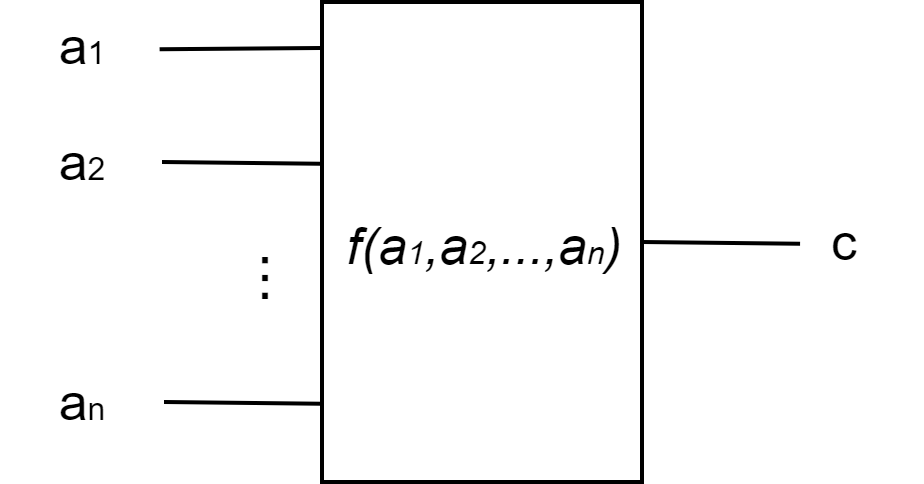
\includegraphics[width=.4\linewidth]{./sdf/classical_mpc/figures/mpc_scheme}
\caption{Multi-Party Computation Diagram}
\label{fig:mpcscheme}
\end{figure}

There are two main models in the literature for the analysis of the Multi-Party Computation problems. The ideal model, which consists in using a Trusted Third Party (TTP). The parties provide their input to the TTP, who will perform the computation of the function. The result is then sent to all the parties. This paradigm relies on the trustworthiness of the TTP because if it turns corrupt, it can supply the private input of one party to the others. This model is extensively used due to its easy implementation and protocols available which prevent the TTP from acting maliciously. The real model of MPC does not use a TTP. In this model, the parties agree on some protocol which will allow them to jointly compute the function. Different protocols are needed for different MPC models and different party behavior models. In \ref{mpcproblemsandsolutions} we will be analyzing different solutions to known MPC problems.

\renewcommand{\figurename}{Figure}
\begin{figure}[H]
\centering
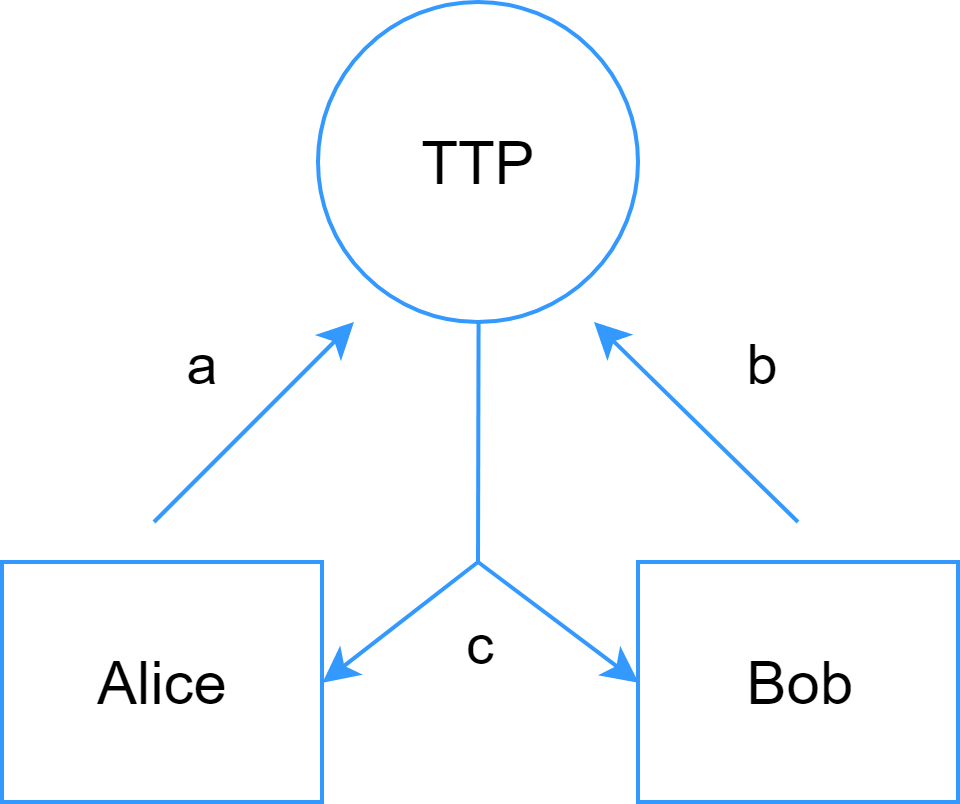
\includegraphics[width=.3\linewidth]{./sdf/classical_mpc/figures/ttp_scheme}
\caption{MPC using a Third Trusted Party}
\label{fig:ttpscheme}
\end{figure}

\subsection{Two-Party Computation}
Two-Party Computation (2PC) is a specific case of MPC, where a generic function \textit{f} receives as input a set $\{a,b\}$
of arguments, where \textit{a} is the input from the first party and \textit{b} is the input from the second,
and outputs a value \textit{c}, as shown in Figure \ref{fig:tpcscheme}.
The output of \textit{f} is given by the following expression.
\begin{equation}\label{eq:tpc}
c = f(a,b)
\end{equation}

\renewcommand{\figurename}{Figure}
\begin{figure}[H]
\centering
\includegraphics[width=.4\linewidth]{./sdf/classical_mpc/figures/two_party_computation_scheme}
\caption{Two-Party Computation Diagram}
\label{fig:tpcscheme}
\end{figure}

\subsection{Party Behavior Models}
There are three main models to describe the behavior of a party. The honest model, where the party follows the protocol and respects the privacy of other parties. A semi honest model, where the party follows the protocol but also tries to gain additional information other than the result. The corrupt model, where the party neither follows the protocol nor respects the privacy of other parties.

\pagebreak

\subsection{MPC Problems and Solutions}\label{mpcproblemsandsolutions}
In this subsection, we will be analyzing different solutions to known MPC problems without the presence of a TTP. We will present a problem and then analyze various solution.

\subsubsection{The Millionaires' Problem}
Consider 2 parties, Alice and Bob, with inputs $a$ and $b$ respectively. The output of this function is $1$ when $a < b$
and $0$ when $a \geq b$. In other terms,
\[
f(a,b) = \left \{
          \begin{tabular}{ccc}
          0, if $a \geq b$ \\
          1, if $a < b$
          \end{tabular}
        \right.
\]
%%%%%%%%%%%%%%%%%%%%%%%%%%%% Solutions Millionaires' Problem %%%%%%%%%%%%%%%%%%%%%%%%%%%%
\paragraph{Yao's Solution}
This method was proposed by Andrew C. Yao in 1982 \cite{yao1982}. Let $E_a$ be Alice's public key, $E_a(x)$ the process of encrypting input $x$ by performing
a bitwise XOR between $x$ and Alice's public key and $D_a(x)$ the process of decrypting input x.
For this example, we will assume the following values: $a = 7$, $b = 3$, $N = 16$, $x = 39226$, $p = 211$ and $E_a = 24698$.

\begin{enumerate}
\item Bob picks a random N-bit integer, $x$, and computes privately the value of $E_a(x)$; calls the result k.
\begin{equation}\label{eq:encryptingX}
k = E_a(x) = x \oplus E_a = 63808
\end{equation}

\item Bob sends Alice the number $k - b + 1$
\begin{equation}\label{eq:encryptingX}
k - b + 1 = 63806
\end{equation}

\item Alice computes privately the values of $Y_u = D_a(k - b + u)$ for $u = 1,2,\ldots,10$\\
\[
Y_u = \begin{bmatrix}
        39236,&39237,&39226,&39227,&39224,&39225,&39230,&39231,&39228,&39229
      \end{bmatrix}
\]

\item Alice generates a random prime $p$ of $N/2$ bits, and computes $Z_u = Y_u$  mod  $p$
\[
Z_u = \begin{bmatrix}
        201,&202,&191,&192,&189,&190,&195,&196,&193,&194
      \end{bmatrix}
\]

\item Alice sends the prime $p$ and the following 10 numbers to Bob: $Z_1,Z_2,\ldots,Z_a$
followed by $Z_{a+1}+1,\ldots,Z_{10}+1$
\[
M = \begin{bmatrix}
        201,&202,&191,&192,&189,&190,&195,&197,&194,&195
      \end{bmatrix}
\]
Note that only the elements of $Z_u$ and $M$ with indexes 7, 8, 9 and 10 are different, since $a = 7$

\item Bob looks at the b-th number sent by Alice, and decides that $a \geq b$ if it is equal to $x$ mod $p$,
and $a < b$ otherwise. In other terms,
\[
f(a,b) = \left \{
          \begin{tabular}{ccc}
          0, if $M_b = x$ mod $p$ \\
          1, if $M_b \ne x$ mod $p$
          \end{tabular}
        \right.
\]
Since $M_b = x$ mod $p = 191$, we have $f(a,b) = 0$, which means that $a \geq b$.
\end{enumerate}
%%%%%%%%%%%%%%%%%%%%%%%%%%%%%%%%%%%%%%%%%%%%%%%%%%%%%%%%%%%%%%%%%%%%%%%%%%%%%%%%%%%%%%%%%%

\subsubsection{1-2 Oblivious Transfer}
Consider 2 parties, Alice and Bob. Alice has a set of messages $A=\{m_0,m_1,m_2,\ldots,m_{n-1}\}$
and Bob has an index $b$. The output of this function should be $m_b$, i.e., the message from Alice's set of index $b$. Bob should not gain any more information other than $m_b$ and Alice should not know the value of $b$.
\begin{equation}\label{eq:messageaccess}
f(A,b) = A_b
\end{equation}

<<<<<<< HEAD
\renewcommand{\figurename}{Figure}
\begin{figure}[H]
\centering
\includegraphics[width=.4\linewidth]{./sdf/classical_mpc/figures/OT}
\caption{Oblivious Transfer Diagram}
\label{fig:otscheme}
\end{figure}

%%%%%%%%%%%%%%%%%%%%%%%%%%%% Solutions 1-2 Oblivious Transfer %%%%%%%%%%%%%%%%%%%%%%%%%%%%



%%%%%%%%%%%%%%%%%%%%%%%%%%%%%%%%%%%%%%%%%%%%%%%%%%%%%%%%%%%%%%%%%%%%%%%%%%%%%%%%%%%%%%%%%%

\subsubsection{Average Value}
Consider 2 parties, Alice and Bob, with inputs $a$ and $b$ respectively. The output of this function should be the average value of $a$ and $b$
. In other terms,
\begin{equation}\label{eq:tpc}
f(a,b) = \frac{a+b}{2}
\end{equation}
=======
\subsubsection{Average Value}
%Complete this section


>>>>>>> Goncalo

%%%%%%%%%%%%%%%%%%%%%%%%%%%%% Solutions Average Value %%%%%%%%%%%%%%%%%%%%%%%%%%%%%%%%%%


%%%%%%%%%%%%%%%%%%%%%%%%%%%%%%%%%%%%%%%%%%%%%%%%%%%%%%%%%%%%%%%%%%%%%%%%%%%%%%%%%%%%%%%%%%
\subsection{Garbled Circuit Protocol}
Introduced in 1986 by Andrew Yao, the Garbled Circuit protocol (GC) addresses the case
of Two-Party Computation (2PC), without the presence of a trusted third party.
GC allows a secure evaluation of a function given as a Boolean circuit that is represented as a series of logic gates.
The circuit is known to both parties.\\

\subsection{Hardware Description Languages}
Contrary to Programming Languages such as C or C++, which are used to specify a set of instructions to a computer, Hardware Description Languages (HDL) are computer languages used to describe the structure and behavior of digital logic circuits. They allow for the synthesis of HDL description code into a netlist (specification of physical eletronic components, such as AND gates or NOT gates, and how they are connected together).

\subsection{TinyGarble}
TinyGarble is a GC framework that takes advantage of powerful logic synthesis techniques, provided by both HDL synthesis tools
and TinyGarble's custom libraries, in order improve the overall efficiency of the GC protocol.
It it possible to describe the circuit using High-Level Programming Languages (HLPL) such as C, although High-Level Synthesis (HLS) is required. HLS is performed by High-Level Synthesis tools, such as SPARK for the C language.

\renewcommand{\figurename}{Figure}
\begin{figure}[H]
\centering
\includegraphics[width=.9\linewidth]{./sdf/classical_mpc/figures/tinygarble_flow_diagram}
\caption{TinyGarble Flow Diagram}
\label{fig:tgdiagram}
\end{figure}

\subsection{ARM2GC}
Although circuit description in HLPL is possible, it is not very efficient when compared to HDL circuit description. ARM2GC addresses this problem, significantly improving the performance of garbled circuits described in HLPL.\\
In the case of 2PC, ARM2GC's approach to GC is based on the ARM processor architecture and consists in providing a public parameter to function \textit{f}, so that its output would be given by the following expression.
\begin{equation}\label{eq:arm2gc}
z = f(a,b,p)
\end{equation}
, where $p$ represents a public parameter, known to both parties.\\
In ARM2GC the Boolean circuit required to perform GC is that of a processor to which the compiled binary of the function is given as a public input ($p$\textit{ = compiled binary of the function}). This optimization is performed by the SkipGate algorithm.



% bibliographic references for the section ----------------------------
\clearpage
\printbibliography[heading=subbibliography]
\end{refsection}
\addcontentsline{toc}{subsection}{Bibliography}
\cleardoublepage
% ---------------------------------------------------------------------  \fi
\ifdefined\quantumMpc   \section{Quantum Multi-Party Computation}

\begin{refsection}

\subsection{Our Approach}
\subsubsection{Message Access}
Let's consider 2 parties, Alice and Bob. Alice has a set $M = \{m_0,m_1\}$ of messages and Bob has the index, $i$, of the message he wants to receive from Alice, $m_i$.\\
For this example we will be assuming that $i=1$ and $M = \{11,10\}$. Both messages are 2-bit binary numbers.
\begin{enumerate}
%%%%%%%%%%%%%%%%%%%%%%%%%%%%%%%%%%%%%%%%%%%%%%%%%%%%%%%%%%%%%%%%%%%%%%%%%%%%%%%%%%%%%%%%%%%%%%%%%%%%%%%%%%%%%%%%%%%%%%%%
\item Bob generates a 4-bit key, $K_b=0111$ where only the bits of indexes $2i$ and $2i+1$ are known ($C$) to him. Since i=1, Bob only knows the last 2 bits of $K_b$. The remaining 2 bits of $K_b$ are random ($R$), thus unknown to Bob.
\renewcommand{\figurename}{Figure}
\begin{figure}[H]
\centering
\includegraphics[width=.25\linewidth]{./figures/mpc/mpc_bob_key}
\caption{Known ($C$) and Unknown ($R$) bits from Bob's perspective }
\label{fig:knownbob}
\end{figure}
%%%%%%%%%%%%%%%%%%%%%%%%%%%%%%%%%%%%%%%%%%%%%%%%%%%%%%%%%%%%%%%%%%%%%%%%%%%%%%%%%%%%%%%%%%%%%%%%%%%%%%%%%%%%%%%%%%%%%%%%
\item Bob sends to Alice the set $I = \{2,3\}$ corresponding to the indexes of the bits known to him.
%%%%%%%%%%%%%%%%%%%%%%%%%%%%%%%%%%%%%%%%%%%%%%%%%%%%%%%%%%%%%%%%%%%%%%%%%%%%%%%%%%%%%%%%%%%%%%%%%%%%%%%%%%%%%%%%%%%%%%%%
\item Alice generates a 4-bit key, $K_a=1011$ where the last 2 bits of $K_a$ must be the same as the last 2 of $K_b$. All 4 bits from the key
are unknown to Alice. She doesn't know which 2 bits from $K_a$ are equal to $K_b$ (only Bob has that information),i.e., from her perspective
all bits are random.
\renewcommand{\figurename}{Figure}
\begin{figure}[H]
\centering
\includegraphics[width=.25\linewidth]{./figures/mpc/mpc_alice_key}
\caption{Known ($C$) and Unknown ($R$) bits from Alice's perspective }
\label{fig:knownalice}
\end{figure}
%%%%%%%%%%%%%%%%%%%%%%%%%%%%%%%%%%%%%%%%%%%%%%%%%%%%%%%%%%%%%%%%%%%%%%%%%%%%%%%%%%%%%%%%%%%%%%%%%%%%%%%%%%%%%%%%%%%%%%%%
\item Alice encrypts the messages with $K_a$ and sends the encrypted information to Bob. In this example, $1101$ will be sent to Bob.
\renewcommand{\figurename}{Figure}
\begin{figure}[H]
\centering
\includegraphics[width=.4\linewidth]{./figures/mpc/mpc_message_encrypting}
\caption{Alice encrypts the messages with $K_a$}
\label{fig:mpcencryption}
\end{figure}
%%%%%%%%%%%%%%%%%%%%%%%%%%%%%%%%%%%%%%%%%%%%%%%%%%%%%%%%%%%%%%%%%%%%%%%%%%%%%%%%%%%%%%%%%%%%%%%%%%%%%%%%%%%%%%%%%%%%%%%%
\item Bob decrypts the information received from Alice with $K_b$ and retrieves the message $m_1$, which correspond to bits of indexes 2 and 3 (since $i=1$).\\
The first two bits of the decrypted information do not represent $m_0$.
\renewcommand{\figurename}{Figure}
\begin{figure}[H]
\centering
\includegraphics[width=.4\linewidth]{./figures/mpc/mpc_message_decrypting}
\caption{Bob decrypts the information with $K_b$}
\label{fig:mpcdecryption}
\end{figure}
\end{enumerate}

\subsubsection{The Millionaire' Problem}
%Complete this section
\subsubsection{Average Value}
%Complete this section



% bibliographic references for the section ----------------------------
\clearpage
\printbibliography[heading=subbibliography]
\end{refsection}
\addcontentsline{toc}{subsection}{Bibliography}
\cleardoublepage
% --------------------------------------------------------------------- \fi
\ifdefined\secureMPC   \input{./sdf/secure_multiparty_computation/secure_multiparty_computation} \fi


% ------------------------------------------------------------------------
\chapter{Library}

\clearpage

\section{ADC}

\begin{tcolorbox}	
	\begin{tabular}{p{2.75cm} p{0.2cm} p{10.5cm}} 	
		\textbf{Header File}   &:& adc$\_*$.h \\
		\textbf{Source File}   &:& adc$\_*$.cpp \\
        \textbf{Version}       &:& 20180423 (Celestino Martins) \\
	\end{tabular}
\end{tcolorbox}

This super block block simulates an analog-to-digital converter (ADC), including signal resample and quantization. It receives two real input signal and outputs two real signal with the sampling rate defined by ADC sampling rate, which is externally configured using the resample function, and quantized signal into a given discrete values.

\subsection*{Input Parameters}

\begin{table}[h]
	\centering
	\begin{tabular}{|c|c|c|c|c|c|cccc}
		\cline{1-4}
		\textbf{Parameter} & \textbf{Unity} & \textbf{Type} & \textbf{Values} &   \textbf{Default}& \\ \cline{1-5}
        samplingPeriod & -- & double & any & $--$ \\ \cline{1-5}
        rFactor       & --    & double & any & $1$ \\ \cline{1-5}	
		resolution & bits  & double & any & $inf$ \\ \cline{1-5}	
        maxValue   & volts & double & any & $1.5$ \\ \cline{1-5}	
        minValue   & volts & double & any    & $-1.5$ \\ \cline{1-5}	
	\end{tabular}
	\caption{ADC input parameters}
	\label{table:ADC_in_par}
\end{table}

\subsection*{Methods}

ADC(vector$<$Signal *$>$ \&InputSig, vector$<$Signal *$>$ \&OutputSig);
\bigbreak
//void setResampleSamplingPeriod(double sPeriod) { B1.setSamplingPeriod(sPeriod); B2.setSamplingPeriod(sPeriod); };
\bigbreak
void setResampleOutRateFactor(double OUTsRate) { B01.setOutRateFactor(OUTsRate); B02.setOutRateFactor(OUTsRate); }
\bigbreak
void setQuantizerSamplingPeriod(double sPeriod) { B03.setSamplingPeriod(sPeriod); B04.setSamplingPeriod(sPeriod); }
\bigbreak
void setSamplingPeriod(double sPeriod) { B03.setSamplingPeriod(sPeriod); };
\bigbreak
void setQuantizerResolution(double nbits) { B03.setResolution(nbits); B04.setResolution(nbits); }
\bigbreak
void setQuantizerMaxValue(double maxvalue) { B03.setMaxValue(maxvalue); B04.setMaxValue(maxvalue);}
\bigbreak
void setQuantizerMinValue(double minvalue) { B03.setMinValue(minvalue); B04.setMinValue(minvalue); }

\subsection*{Functional description}

This super block is composed of two blocks, resample and quantizer. It can perform the signal resample according to the defined input parameter \textit{rFactor} and signal quantization according to the defined input parameter \textit{nBits}.


\pagebreak
\subsection*{Input Signals}

\subparagraph*{Number:} 2

\subsection*{Output Signals}

\subparagraph*{Number:} 2

\subparagraph*{Type:} Electrical complex signal

\subsection*{Examples}

\subsection*{Sugestions for future improvement}



\clearpage

\section{Add}

\begin{tcolorbox}	
\begin{tabular}{p{2.75cm} p{0.2cm} p{10.5cm}} 	
\textbf{Header File}   &:& add.h \\
\textbf{Source File}   &:& add.cpp \\
\textbf{Version}       &:& 20180118
\end{tabular}
\end{tcolorbox}

\subsection*{Input Parameters}

This block takes no parameters.

\subsection*{Functional Description}

This block accepts two signals and outputs one signal built from a sum of the two inputs. The input and output signals must be of the same type, if this is not the case the block returns an error.

\subsection*{Input Signals}

\textbf{Number}: 2\\
\textbf{Type}: Real, Complex or Complex\_XY signal (ContinuousTimeContinuousAmplitude)

\subsection*{Output Signals}

\textbf{Number}: 1\\
\textbf{Type}: Real, Complex or Complex\_XY signal (ContinuousTimeContinuousAmplitude)

%\end{document}

\clearpage

\section{Balanced Beam Splitter}

\begin{tcolorbox}	
\begin{tabular}{p{2.75cm} p{0.2cm} p{10.5cm}} 	
\textbf{Header File}   &:& balanced\_beam\_splitter.h \\
\textbf{Source File}   &:& balanced\_beam\_splitter.cpp \\
\textbf{Version}       &:& 20180124
\end{tabular}
\end{tcolorbox}

\subsection*{Input Parameters}

\begin{table}[H]
\centering
\begin{tabular}{|l|l|l|}
\hline
Name           & Type    & Default Value     \\ \hline
Matrix         & array <t\_complex, 4> & $\lbrace~\lbrace \frac{1}{\sqrt{2}},~\frac{1}{\sqrt{2}},~\frac{1}{\sqrt{2}},~\frac{-1}{\sqrt{2}} \rbrace~\rbrace$                             \\ \hline
Mode           & double  & 0                 \\ \hline
\end{tabular}
\end{table}

\subsection*{Functional Description}
The structure of the beam splitter can be controlled with the parameter mode.\\
When \textbf{Mode = 0} the beam splitter will have one input port and two output ports - \textbf{1x2 Beam Splitter}. If Mode has a value different than 0, the splitter will have two input ports and two output ports - \textbf{2x2 Beam Splitter}.\\
Considering the first case, the matrix representing a 2x2 Beam Splitter can be summarized in the following way,

\begin{equation}
M_{BS}=~\frac{\sqrt{2}}{2}\begin{bmatrix}
              					1  & 1 \\
            					1 & -1
            			  \end{bmatrix}
\end{equation}
The relation between the values of the input ports and the values of the output ports can be established in the following way

\begin{equation}
\begin{bmatrix}
A' \\
B'
\end{bmatrix}=M_{BS} \dot{}{\begin{bmatrix}
			  				     A \\
			  	                 B
			  	                 \end{bmatrix}}
\end{equation}
Where, A and B represent the inputs and A' and B' represent the outputs of the Beam Splitter.

\subsection*{Input Signals}

\textbf{Number}: 1 or 2\\
\textbf{Type}: Complex

\subsection*{Output Signals}

\textbf{Number}: 2\\
\textbf{Type}: Complex




%%%%%%%%%%%%%%%%%%%%%%%%%%%%%%%%%%%%%%%%%%%%%%%%%%%%%%%%%%%%%%%%%%%%%%%%%%%%%%%%%%%%%%%%%%%%%%%%%%%%%%%%%%%%
% References
%%%%%%%%%%%%%%%%%%%%%%%%%%%%%%%%%%%%%%%%%%%%%%%%%%%%%%%%%%%%%%%%%%%%%%%%%%%%%%%%%%%%%%%%%%%%%%%%%%%%%%%%%%%%

%\renewcommand{\bibname}{References}
%
%\bibliographystyle{unsrt}
% argument is your BibTeX string definitions and bibliography database(s)
%\bibliography{./lib/balanced_beam_splitter/balanced_beam_splitter}
%
%


\clearpage

\section{Bit Error Rate}

\begin{refsection}

\begin{tcolorbox}	
\begin{tabular}{p{2.75cm} p{0.2cm} p{10.5cm}} 	
\textbf{Header File}   &:& bit\_error\_rate\_*.h \\
\textbf{Source File}   &:& bit\_error\_rate\_*.cpp \\
\textbf{Version}       &:& 20171810 (Daniel Pereira)
\end{tabular}
\end{tcolorbox}

\subsection*{Input Parameters}

\begin{table}[H]
\centering
\begin{tabular}{|l|l|l|}
\hline
Name           & Type           & Default Value     \\ \hline
alpha          & double         & 0.05              \\ \hline
m              & integer        & 0                 \\ \hline
lMinorant      & double         & $1\times10^{-10}$ \\ \hline
\end{tabular}
\end{table}

\begin{tcolorbox}	
\begin{tabular}{p{2.75cm} p{0.2cm} p{10.5cm}} 	
\textbf{Version}       &:& 20181424 (Mariana Ramos)
\end{tabular}
\end{tcolorbox}

\begin{table}[H]
\centering
\begin{tabular}{|l|l|l|}
\hline
Name           & Type           & Default Value     \\ \hline
alpha          & double         & 0.05              \\ \hline
m              & integer        & 0                 \\ \hline
lMinorant      & double         & $1\times10^{-10}$ \\ \hline
midRepType     & MidReportType  & Cumulative \\ \hline
\end{tabular}
\end{table}

\subsection*{Methods}

\begin{itemize}
  \item BitErrorRate(vector<Signal *> \&InputSig, vector<Signal *> \&OutputSig) :Block(InputSig,OutputSig)\{\};
  \item void initialize(void);
  \item bool runBlock(void);
  \item void setConfidence(double P) \{ alpha = 1-P; \}
  \item void setMidReportSize(int M) \{ m = M; \}
  \item void setLowestMinorant(double lMinorant) \{ lowestMinorant=lMinorant; \}
\end{itemize}

\begin{tcolorbox}	
\begin{tabular}{p{2.75cm} p{0.2cm} p{10.5cm}} 	
\textbf{Version}       &:& 20181424 (Mariana Ramos)
\end{tabular}
\end{tcolorbox}

\begin{itemize}
  \item BitErrorRate(vector<Signal *> \&InputSig, vector<Signal *> \&OutputSig) :Block(InputSig,OutputSig)\{\};
  \item void initialize(void);
  \item bool runBlock(void);
  \item void setConfidence(double P) \{ alpha = 1-P; \}
  \item void setMidReportSize(int M) \{ m = M; \}
  \item void setLowestMinorant(double lMinorant) \{ lowestMinorant=lMinorant; \}
  \item void setMidReportType(MidReportType mrt) \{ midRepType = mrt; \};
\end{itemize}

\subsection*{Input Signals}

\textbf{Number}: 2\\
\textbf{Type}: Binary (DiscreteTimeDiscreteAmplitude)


\subsection*{Output Signals}

\textbf{Number}: 1\\
\textbf{Type}: Binary (DiscreteTimeDiscreteAmplitude)

\subsection*{Functional Description}

This block accepts two binary strings and outputs a binary string, outputting a 1 if the two input samples are equal to each other and 0 if not. This block also outputs \textit{.txt} files with a report of the estimated Bit Error Rate (BER), $\widehat{\text{BER}}$ as well as the estimated confidence bounds for a given probability $\alpha$.
\par
The block allows for mid-reports to be generated, the number of bits between reports is customizable, if it is set to 0 then the block will only output the final report. In version \textbf{20180424} this block can operate mid-reports using a CUMULATIVE mode, in which the BER is calculated in a cumulative way taking into account all received bits, coincidences and errors, or in a RESET mode, in which at each \textbf{m} bits the number of received bits and coincidence bits is reset for the BER calculation.

\subsection*{Theoretical Description}\label{bercalc}
The $\widehat{\text{BER}}$ is obtained by counting both the total number received bits, $N_T$, and the number of coincidences, $K$, and calculating their relative ratio:
\begin{equation}
\widehat{\text{BER}}=1-\frac{K}{N_T}.
\end{equation}
The upper and lower bounds, $\text{BER}_\text{UB}$ and $\text{BER}_\text{LB}$ respectively, are calculated using the Clopper-Pearson confidence interval, which returns the following simplified expression for $N_T>40$~\cite{Almeida16}:
\begin{align}
\text{BER}_\text{UB}&=\widehat{\text{BER}}+\frac{1}{\sqrt{N_T}}z_{\alpha/2}\sqrt{\widehat{\text{BER}}(1-\widehat{\text{BER}})}+\frac{1}{3N_T}\left[2\left(\frac{1}{2}-\widehat{\text{BER}}\right)z_{\alpha/2}^2+(2-\widehat{\text{BER}})\right]\\
\text{BER}_\text{LB}&=\widehat{\text{BER}}-\frac{1}{\sqrt{N_T}}z_{\alpha/2}\sqrt{\widehat{\text{BER}}(1-\widehat{\text{BER}})}+\frac{1}{3N_T}\left[2\left(\frac{1}{2}-\widehat{\text{BER}}\right)z_{\alpha/2}^2-(1+\widehat{\text{BER}})\right],
\end{align}
where $z_{\alpha/2}$ is the $100\left(1-\frac{\alpha}{2}\right)$th percentile of a standard normal distribution.



% bibliographic references for the section ----------------------------
\clearpage
\printbibliography[heading=subbibliography]
\end{refsection}
\addcontentsline{toc}{subsection}{Bibliography}
\cleardoublepage
% --------------------------------------------------------------------- 
\clearpage

\section{Binary Source}

\begin{tcolorbox}	
	\begin{tabular}{p{2.75cm} p{0.2cm} p{10.5cm}} 	
		\textbf{Header File}   &:& binary\_source.h \\
		\textbf{Source File}   &:& binary\_source.cpp \\
	\end{tabular}
\end{tcolorbox}

\maketitle
This block generates a sequence of binary values (1 or 0) and it can work in four different modes:

\begin{multicols}{2}
\begin{enumerate}
	\item Random
	\item PseudoRandom
	\item DeterministicCyclic
	\item DeterministicAppendZeros
\end{enumerate}
\end{multicols}

This blocks doesn't accept any input signal. It produces any number of output signals.

\subsection*{Input Parameters}

%	\begin{itemize}
%		\item mode\{PseudoRandom\}\linebreak
%		(Random, PseudoRandom, DeterministicCyclic, DeterministicAppendZeros)
%		\item probabilityOfZero\{0.5\}\linebreak
%		(real $\in$ [0,1])
%		\item patternLength\{7\} \linebreak
%		(integer $\in$ [1,32])
%		\item bitStream\{"0100011101010101"\} \linebreak
%		(string of 0's and 1's)
%		\item numberOfBits\{-1\} \linebreak
%		(long int)
%		\item bitPeriod\{1.0/100e9\} \linebreak
%		(double)
%	\end{itemize}

\begin{table}[h]
	\centering
	\begin{tabular}{|c|c|p{60mm}|c|ccp{60mm}}
		\cline{1-4}
		\textbf{Parameter} & \textbf{Type} & \textbf{Values} &   \textbf{Default}& \\ \cline{1-4}
		mode & string & Random, PseudoRandom, DeterministicCyclic, DeterministicAppendZeros & PseudoRandom \\ \cline{1-4}
		probabilityOfZero & real & $\in$ [0,1] & 0.5 \\ \cline{1-4}
		patternLength & int &  Any natural number & 7 \\ \cline{1-4}
		bitStream & string & sequence of 0's and 1's & 0100011101010101 \\ \cline{1-4}
		numberOfBits & long int & any & -1 \\ \cline{1-4}
		bitPeriod & double & any & $1.0/100e9$ \\ \cline{1-4}
	\end{tabular}
	\caption{Binary source input parameters}
	\label{table:bin_sour_in_par}
\end{table}

\subsection*{Methods}

BinarySource(vector$\langle$Signal *$\rangle$ \&InputSig, vector$\langle$Signal *$\rangle$ \&OutputSig) :Block(InputSig, OutputSig)\{\};
\bigbreak	
void initialize(void);
\bigbreak	
bool runBlock(void);
\bigbreak	
void setMode(BinarySourceMode m)
BinarySourceMode const getMode(void)
\bigbreak	
void setProbabilityOfZero(double pZero)
\bigbreak
double const getProbabilityOfZero(void)
\bigbreak	
void setBitStream(string bStream)
\bigbreak
string const getBitStream(void)
\bigbreak	
void setNumberOfBits(long int nOfBits)
\bigbreak
long int const getNumberOfBits(void)
\bigbreak	
void setPatternLength(int pLength)
\bigbreak
int const getPatternLength(void)
\bigbreak	
void setBitPeriod(double bPeriod)
\bigbreak
double const getBitPeriod(void)

\subsection*{Functional description}

The \textit{mode} parameter allows the user to select between one of the four operation modes of the binary source.

\subparagraph*{Random Mode}
Generates a 0 with probability \textit{probabilityOfZero} and a 1 with probability 1-\textit{probabilityOfZero}.

\subparagraph*{Pseudorandom Mode}
Generates a pseudorandom sequence with period $2^\textit{patternLength}-1$.

\subparagraph*{DeterministicCyclic Mode}
Generates the sequence of 0's and 1's specified by \textit{bitStream} and then repeats it.

\subparagraph*{DeterministicAppendZeros Mode}
Generates the sequence of 0's and 1's specified by \textit{bitStream} and then it fills the rest of the buffer space with zeros.

\subsection*{Input Signals}


\subparagraph*{Number:} 0

\subparagraph*{Type:} Binary (DiscreteTimeDiscreteAmplitude)

\subsection*{Output Signals}

\subparagraph*{Number:} 1 or more

\subparagraph*{Type:} Binary (DiscreteTimeDiscreteAmplitude)

\subsection*{Examples}

\paragraph*{Random Mode}

\paragraph*{PseudoRandom Mode}
As an example consider a pseudorandom sequence with \textit{patternLength}=3 which contains a total of 7 ($2^3-1$) bits. In this sequence it is possible to find every combination of 0's and 1's that compose a 3 bit long subsequence with the exception of $000$. For this example the possible subsequences are $010$, $110$, $101$, $100$, $111$, $001$ and $100$ (they appear in figure \ref{BinarySequenceN3} numbered in this order). Some of these require wrap.

\begin{figure}[h]
	\centering
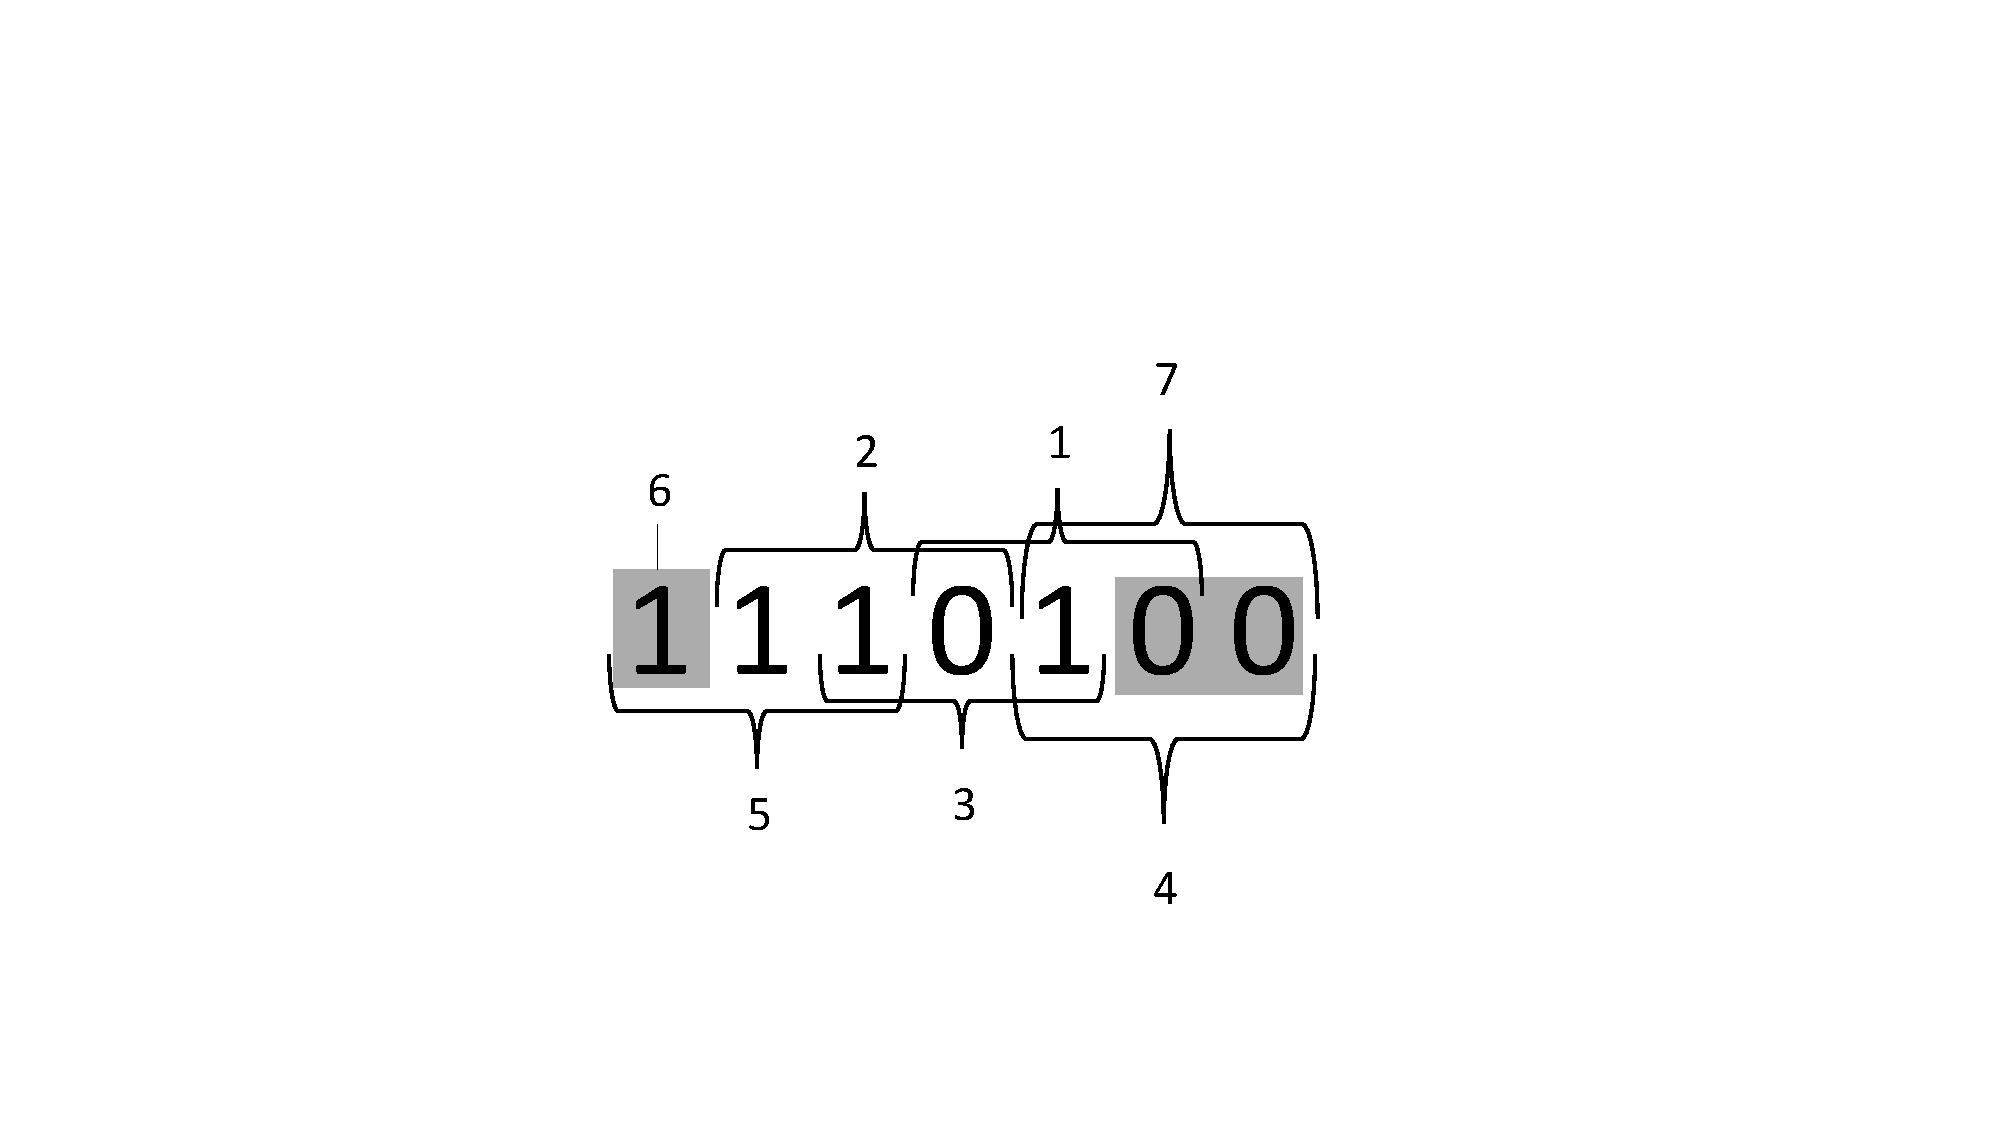
\includegraphics[width=\textwidth]{./lib/binary_source/figures/BinarySequenceN3.pdf}
\caption{Example of a pseudorandom sequence with a pattern length equal to 3.}\label{BinarySequenceN3}
\end{figure}

\paragraph*{DeterministicCyclic Mode}

As an example take the \textit{bit stream} '0100011101010101'. The generated binary signal is displayed in.

\paragraph*{DeterministicAppendZeros Mode}

Take as an example the \textit{bit stream} '0100011101010101'. The generated binary signal is displayed in \ref{MQAM1_DeterministAppendZeros}.

\begin{figure}
	\centering
	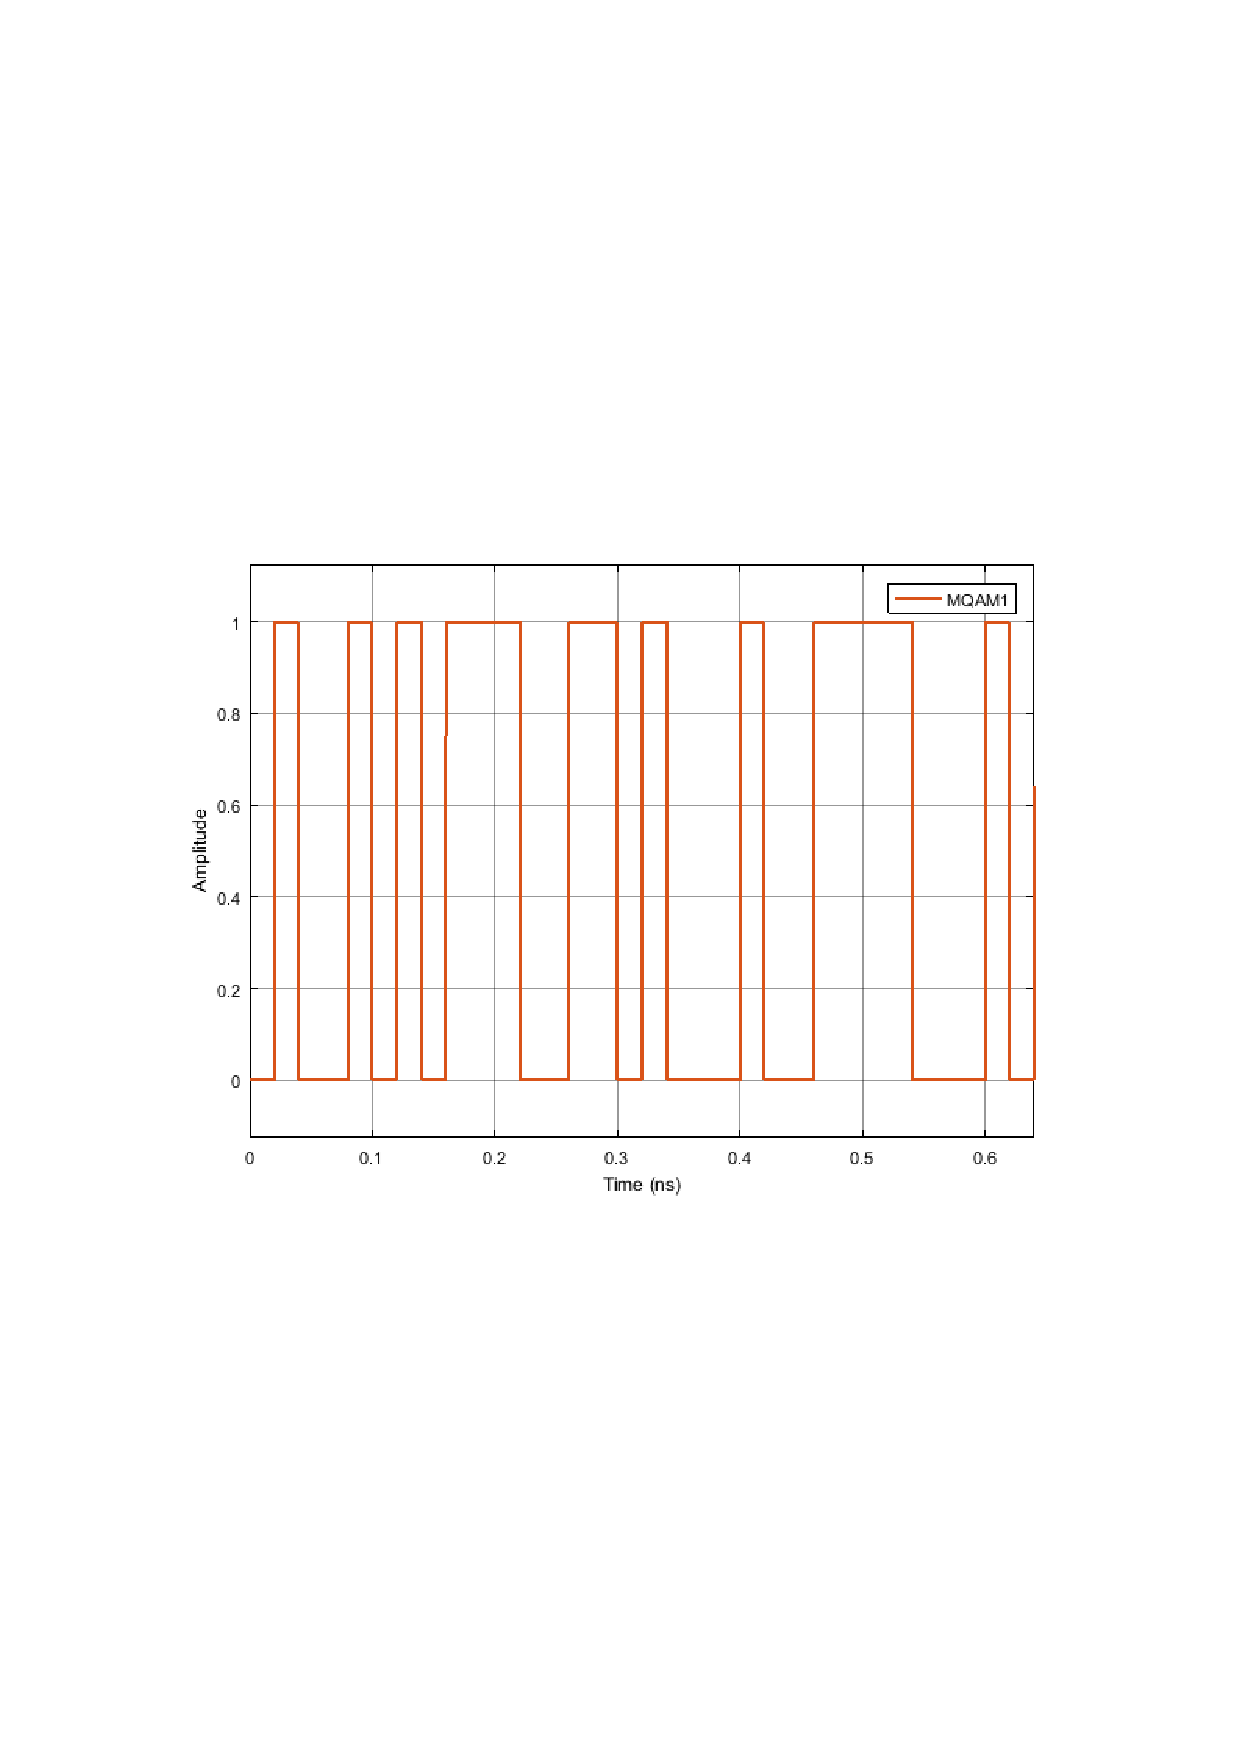
\includegraphics[clip, trim=0.5cm 9cm 0.5cm 9cm, width=\textwidth]{./lib/binary_source/figures/BinarySource_output.pdf}
	
	\caption{Binary signal generated by the block operating in the \textit{Deterministic Append Zeros} mode with a binary sequence 01000...}\label{MQAM1_DeterministAppendZeros}
\end{figure}

\subsection*{Sugestions for future improvement}

Implement an input signal that can work as trigger.


\clearpage

\section{Bit Decider}

\begin{tcolorbox}	
\begin{tabular}{p{2.75cm} p{0.2cm} p{10.5cm}} 	
\textbf{Header File}   &:& bit\_decider.h \\
\textbf{Source File}   &:& bit\_decider.cpp \\
\textbf{Version}       &:& 20170818
\end{tabular}
\end{tcolorbox}

\subsection*{Input Parameters}

\begin{table}[H]
\centering
\begin{tabular}{|l|l|l|}
\hline
Name           & Type   & Default Value     \\ \hline
decisionLevel  & double &  0.0              \\ \hline
\end{tabular}
\end{table}

\subsection*{Functional Description}

This block accepts one real discrete signal and outputs a binary string, outputting a 1 if the input sample is greater than the decision level and 0 if it is less or equal to the decision level.

\subsection*{Input Signals}

\textbf{Number}: 1

\textbf{Type}: Real signal (DiscreteTimeContinuousAmplitude)

\subsection*{Output Signals}

\textbf{Number}: 1

\textbf{Type}: Binary (DiscreteTimeDiscreteAmplitude)

\clearpage

\section{Clock}

\begin{tcolorbox}	
	\begin{tabular}{p{2.75cm} p{0.2cm} p{10.5cm}} 	
		\textbf{Header File}   &:& clock.h \\
		\textbf{Source File}   &:& clock.cpp \\
	\end{tabular}
\end{tcolorbox}

This block doesn't accept any input signal. It outputs one signal that corresponds to a sequence of Dirac's delta functions with a user defined \textit{period}.

\subsection*{Input Parameters}

%\begin{itemize}
%	\item period\{ 0.0 \};
%	\item samplingPeriod\{ 0.0 \};
%\end{itemize}

\begin{table}[h]
	\centering
	\begin{tabular}{|c|c|c|c|cccc}
		\cline{1-4}
		\textbf{Parameter} & \textbf{Type} & \textbf{Values} &   \textbf{Default}& \\ \cline{1-4}
		period & double & any & $0.0$ \\ \cline{1-4}
		samplingPeriod & double & any & $0.0$ \\ \cline{1-4}
	\end{tabular}
	\caption{Binary source input parameters}
	\label{table:clock_in_par}
\end{table}

\subsection*{Methods}

Clock() {}
\bigbreak
Clock(vector$<$Signal *$>$ \&InputSig, vector$<$Signal *$>$ \&OutputSig) :Block(InputSig, OutputSig) {}
\bigbreak
void initialize(void)
\bigbreak
bool runBlock(void)
\bigbreak
void setClockPeriod(double per)
\bigbreak
void setSamplingPeriod(double sPeriod)

\subsection*{Functional description}


\pagebreak

\subsection*{Input Signals}

\subparagraph*{Number:} 0

\subsection*{Output Signals}

\subparagraph*{Number:} 1

\subparagraph*{Type:} Sequence of Dirac's delta functions. (TimeContinuousAmplitudeContinuousReal)

\subsection*{Examples}

%\begin{figure}[h]
%	\centering
%	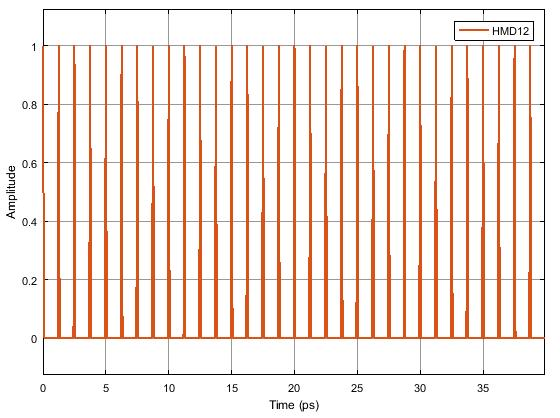
\includegraphics[width=\textwidth]{./lib/clock/figures/Clock_output}
%	\caption{Example of the output signal of the clock}\label{Clock_output}
%\end{figure}

\subsection*{Sugestions for future improvement}


\clearpage

\section{Clock\_20171219}

This block doesn't accept any input signal. It outputs one signal that corresponds to a sequence of Dirac's delta functions with a user defined \textit{period}, \textit{phase} and \textit{sampling period}.

\subsection*{Input Parameters}

\begin{itemize}
	\item period\{ 0.0 \};
	\item samplingPeriod\{ 0.0 \};
    \item phase \{0.0\};
\end{itemize}

\subsection*{Methods}

Clock() {}
\bigbreak
Clock(vector$<$Signal *$>$ \&InputSig, vector$<$Signal *$>$ \&OutputSig) :Block(InputSig, OutputSig) {}
\bigbreak
void initialize(void)
\bigbreak
bool runBlock(void)
\bigbreak
void setClockPeriod(double per)
double getClockPeriod()
\bigbreak
void setClockPhase(double pha)
double getClockPhase()
\bigbreak
void setSamplingPeriod(double sPeriod)
double getSamplingPeriod()

\subsection*{Functional description}


\subsection*{Input Signals}

\subparagraph*{Number:} 0

\subsection*{Output Signals}

\subparagraph*{Number:} 1

\subparagraph*{Type:} Sequence of Dirac's delta functions. (TimeContinuousAmplitudeContinuousReal)

\subsection*{Examples}

\begin{figure}[h]
	\centering
	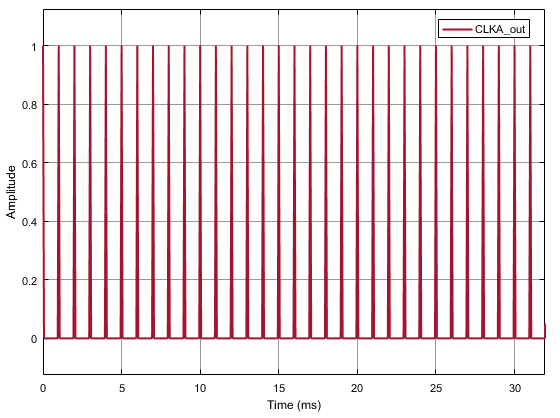
\includegraphics[width=\textwidth]{./lib/clock_20171219/figures/clock_withoutpha}
	\caption{Example of the output signal of the clock without phase shift.}
\end{figure}

\begin{figure}[h]
	\centering
	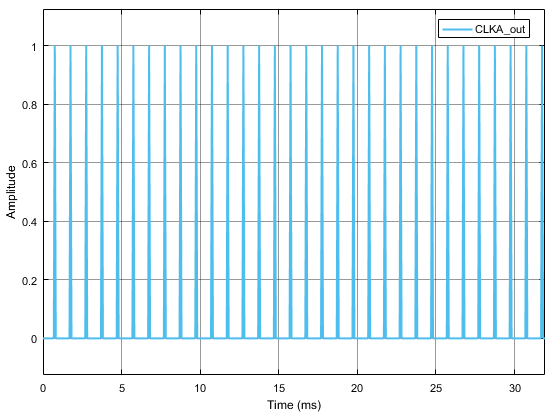
\includegraphics[width=\textwidth]{./lib/clock_20171219/figures/clockPhased}
	\caption{Example of the output signal of the clock with phase shift.}
\end{figure}

\subsection*{Sugestions for future improvement}


\input{./lib/coupler_2_by_2/coupler_2_by_2}
\clearpage

\section{Carrier Phase Compensation}

\begin{tcolorbox}	
	\begin{tabular}{p{2.75cm} p{0.2cm} p{10.5cm}} 	
		\textbf{Header File}   &:& cpe$\_*$.h \\
		\textbf{Source File}   &:& cpe$\_*$.cpp \\
        \textbf{Version}       &:& 20180423 (Celestino Martins) \\
	\end{tabular}
\end{tcolorbox}

This block performs the laser phase noise compensation using either Viterbi-Viterbi (VV) algorithm or blind phase search algorithm (BPS). For both cases, it receives one input complex signal and outputs one complex signal.

\subsection*{Input Parameters For VV Algorithms}

\begin{table}[h]
	\centering
	\begin{tabular}{|c|c|c|c|cccc}
		\cline{1-4}
		\textbf{Parameter} & \textbf{Type} & \textbf{Values} &   \textbf{Default}& \\ \cline{1-4}
		nTaps              & int & any & $25$ \\ \cline{1-4}
        methodType         & string & VV & VV \\ \cline{1-4}
		samplingPeriod     & double & any & $0.0$ \\ \cline{1-4}	
        symbolPeriod       & double & any & $0.0$ \\ \cline{1-4}	
	\end{tabular}
	\caption{CPE input parameters}
	\label{table:cpe_in_par_vv}
\end{table}


\subsection*{Input Parameters For BPS Algorithms}

\begin{table}[h]
	\centering
	\begin{tabular}{|c|c|c|c|cccc}
		\cline{1-4}
		\textbf{Parameter} & \textbf{Type} & \textbf{Values} &   \textbf{Default}& \\ \cline{1-4}
		nTaps              & int & any & $25$ \\ \cline{1-4}
        NtestPhase         & int & any & $32$ \\ \cline{1-4}
        methodType         & string & BPS & VV \\ \cline{1-4}
		samplingPeriod     & double & any & $0.0$ \\ \cline{1-4}	
        symbolPeriod       & double & any & $0.0$ \\ \cline{1-4}	
	\end{tabular}
	\caption{CPE input parameters}
	\label{table:cpe_in_par_bps}
\end{table}

\subsection*{Methods}

CPE() {};
\bigbreak
CPE(vector$<$Signal *$>$ \&InputSig, vector$<$Signal *$>$ \&OutputSig) :Block(InputSig, OutputSig)\{\};
\bigbreak
void initialize(void);
\bigbreak
bool runBlock(void);
\bigbreak
void setSamplingPeriod(double sPeriod) { samplingPeriod = sPeriod; }
\bigbreak
void setSymbolPeriod(double sPeriod) { symbolPeriod = sPeriod; }
\bigbreak
void setnTaps(double ntaps) { nTaps = ntaps; }
\bigbreak
double getnTaps() { return nTaps; }
\bigbreak
void setTestPhase(double nTphase) { nTestPhase = nTphase; }
\bigbreak
double getTestPhase() { return nTestPhase; }
\bigbreak
void setmethodType(string mType) { methodType = mType; }
\bigbreak
double getmethodType() { return methodType; }

\subsection*{Functional description}

This block can perform the carrier phase noise compensation originated by the laser source and local oscillator in coherent optical communication systems. For the sake of simplicity, in this simulation we have restricted all the phase noise at the transmitter side, in this case generated by the laser source, which is then compensated at the receiver side using DSP algorithms.
In this simulation, the carrier phase noise compensation can be performed by applying either the well known Viterbi-Viterbi (VV) algorithm or blind phase search algorithm (BPS), by configuring the parameter $methodType$. The parameter $methodType$ is defined as a string type and it can be configured as: i) When the parameter $methodType$ is $\textit{VV}$ it is applied the VV algorithm; When the parameter $methodType$ is $\textit{BPS}$ it is applied the BPS algorithm.


\pagebreak
\subsection*{Input Signals}

\subparagraph*{Number:} 1

\subsection*{Output Signals}

\subparagraph*{Number:} 1

\subparagraph*{Type:} Electrical complex signal

\subsection*{Examples}

\subsection*{Sugestions for future improvement}



\clearpage

\section{Decoder}

\begin{tcolorbox}	
	\begin{tabular}{p{2.75cm} p{0.2cm} p{10.5cm}} 	
		\textbf{Header File}   &:& decoder.h \\
		\textbf{Source File}   &:& decoder.cpp \\
	\end{tabular}
\end{tcolorbox}


This block accepts a complex electrical signal and outputs a sequence of binary values (0's and 1's). Each point of the input signal corresponds to a pair of bits.

\subsection*{Input Parameters}

%\begin{itemize}
%	\item\texttt{t\_integer} m\{ 4 \}
%	\item vector$<$\texttt{t\_complex}$>$ iqAmplitudes\{ \{ 1.0, 1.0 \},\{ -1.0, 1.0 \},\{ -1.0, -1.0 \},\{ 1.0, -1.0 \} \};
%\end{itemize}


\begin{table}[h]
	\centering
	\begin{tabular}{|c|c|c|c|ccp{60mm}}
		\cline{1-4}
		\textbf{Parameter} & \textbf{Type} & \textbf{Values} &   \textbf{Default}& \\ \cline{1-4}
		m & int & $\geq 4$ & $4$ \\ \cline{1-4}
		iqAmplitudes & vector$<$\texttt{t\_complex}$>$ & \---- & \{ \{ 1.0, 1.0 \},\{ -1.0, 1.0 \},\{ -1.0, -1.0 \},\{ 1.0, -1.0 \} \} \\ \cline{1-4}
	\end{tabular}
	\caption{Binary source input parameters}
	\label{table:decoder_in_par}
\end{table}

\subsection*{Methods}

Decoder() {}
\bigbreak
Decoder(vector$<$Signal *$>$ \&InputSig, vector$<$Signal *$>$ \&OutputSig) :Block(InputSig, OutputSig) {}
\bigbreak
void initialize(void)
\bigbreak
bool runBlock(void)
\bigbreak
void setM(int mValue)
\bigbreak
void getM()
\bigbreak
void setIqAmplitudes(vector$<$\texttt{t\_iqValues}$>$ iqAmplitudesValues)
\bigbreak
vector$<$\texttt{t\_iqValues}$>$getIqAmplitudes()

\subsection*{Functional description}

This block makes the correspondence between a complex electrical signal and pair of binary values using a predetermined constellation.

To do so it computes the distance in the complex plane between each value of the input signal and each value of the \textit{iqAmplitudes} vector selecting only the shortest one. It then converts the point in the IQ plane to a pair of bits making the correspondence between the input signal and a pair of bits.

\pagebreak

\subsection*{Input Signals}

\subparagraph*{Number:} 1

\subparagraph*{Type:} Electrical complex (TimeContinuousAmplitudeContinuousReal)

\subsection*{Output Signals}

\subparagraph*{Number:} 1

\subparagraph*{Type:} Binary

\subsection*{Examples}

As an example take an input signal with positive real and imaginary parts. It would correspond to the first point of the \textit{iqAmplitudes} vector and therefore it would be associated to the  pair of bits $00$.

\begin{figure}[h]
	\centering
	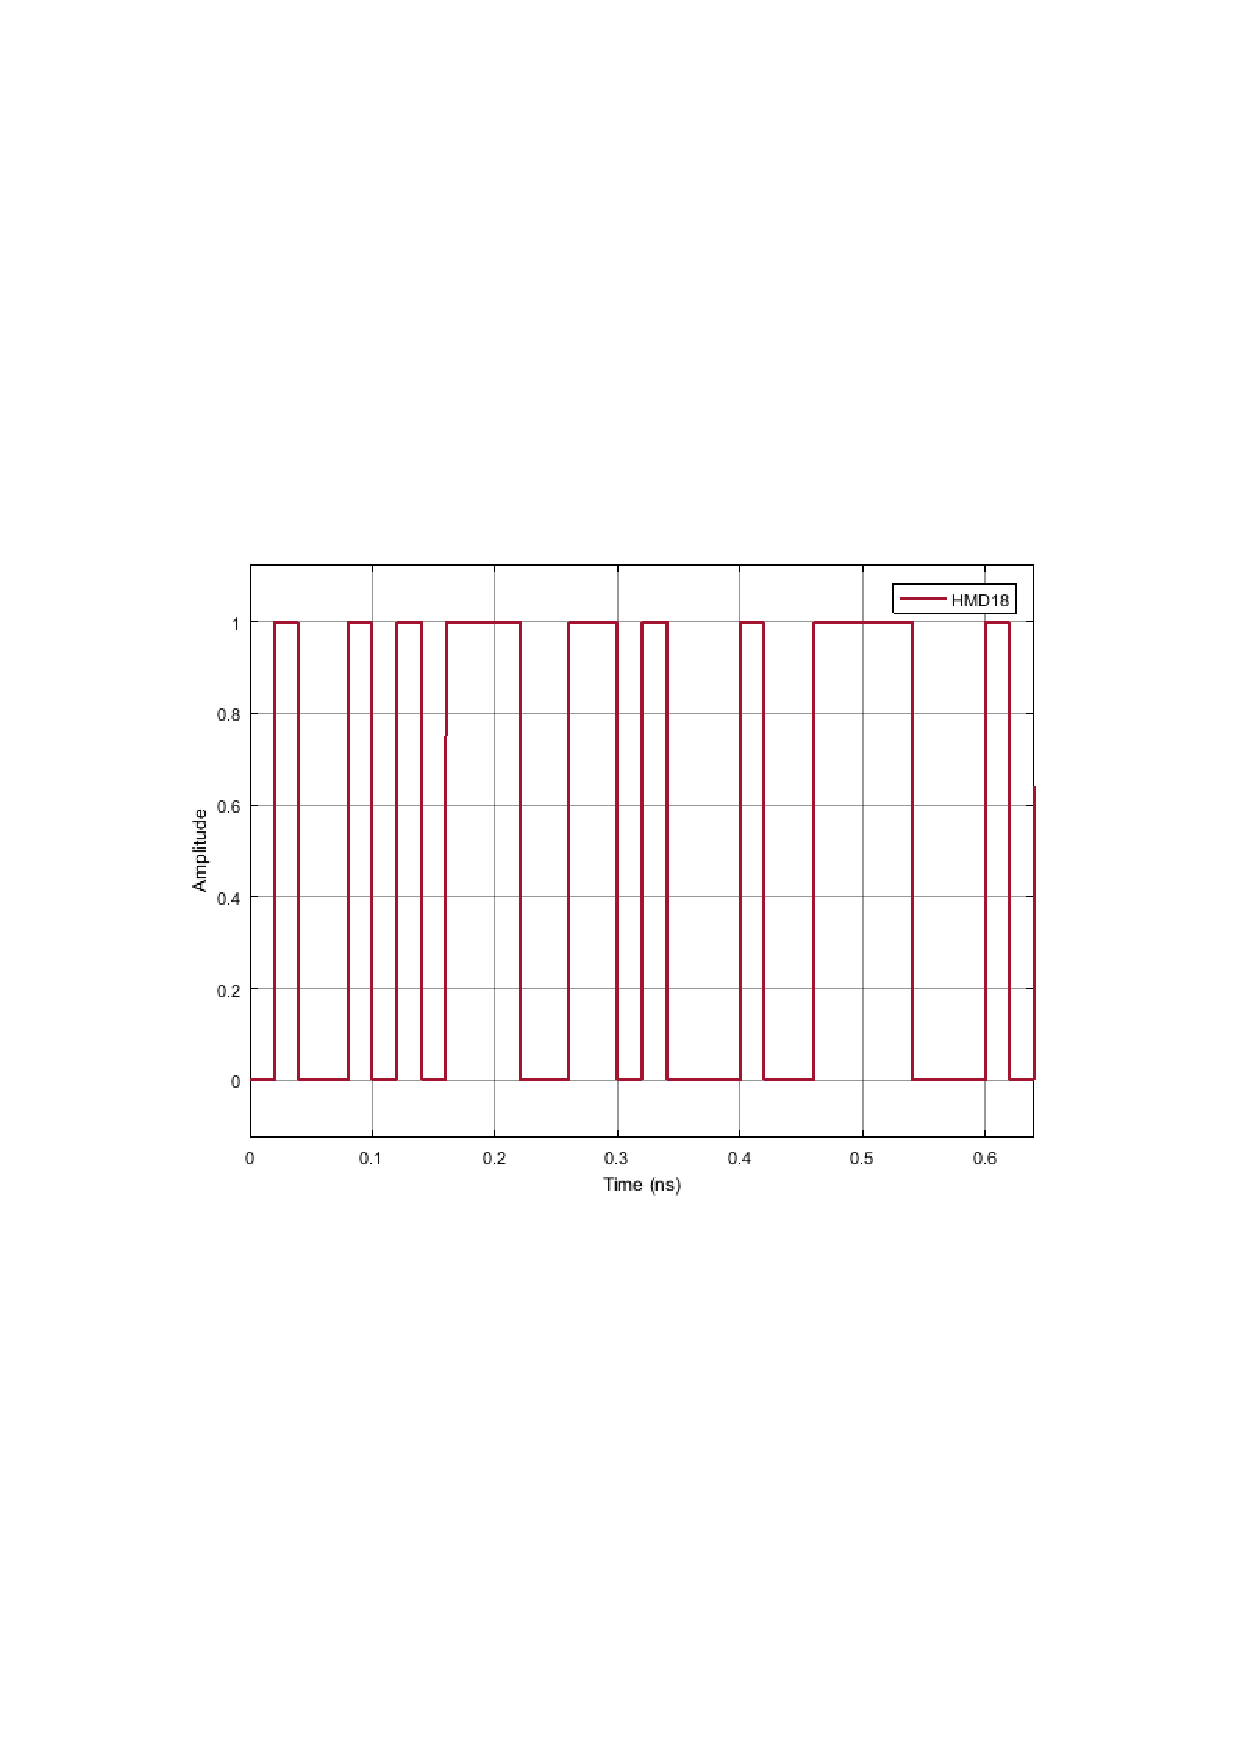
\includegraphics[clip, trim=0.5cm 9cm 0.5cm 9cm, width=\textwidth]{./lib/decoder/figures/MQAM_decoder_output.pdf}
	\caption{Example of the output signal of the decoder for a binary sequence 01. As expected it reproduces the initial bit stream}\label{Decoder_output}
\end{figure}

\subsection*{Sugestions for future improvement}

\clearpage

\section{Discrete To Continuous Time}

\begin{tcolorbox}	
	\begin{tabular}{p{2.75cm} p{0.2cm} p{10.5cm}} 	
		\textbf{Header File}   &:& discrete\_to\_continuous\_time.h \\
		\textbf{Source File}   &:& discrete\_to\_continuous\_time.cpp \\
	\end{tabular}
\end{tcolorbox}

This block converts a signal discrete in time to a signal continuous in time. It accepts one input signal that is a sequence of 1's and -1's and it produces one output signal that is a sequence of Dirac delta functions.

\subsection*{Input Parameters}

\begin{table}[h]
	\centering
	\begin{tabular}{|c|c|c|c|cccc}
		\cline{1-4}
		\textbf{Parameter} & \textbf{Type} & \textbf{Values} &   \textbf{Default}& \\ \cline{1-4}
		numberOfSamplesPerSymbol & int & any & $8$ \\ \cline{1-4}
	\end{tabular}
	\caption{Binary source input parameters}
	\label{table:disc2cont_in_par}
\end{table}

%\begin{itemize}
%	\item numberOfSamplesPerSymbol\{8\} \linebreak
%	(int)
%\end{itemize}

\subsection*{Methods}

DiscreteToContinuousTime(vector$<$Signal *$>$ \&inputSignals, vector$<$Signal *$>$ \&outputSignals) :Block(inputSignals, outputSignals)\{\};
\bigbreak	
void initialize(void);
\bigbreak	
bool runBlock(void);
\bigbreak	
void setNumberOfSamplesPerSymbol(int nSamplesPerSymbol)
\bigbreak
int const getNumberOfSamplesPerSymbol(void)

\subsection*{Functional Description}

This block reads the input signal buffer value, puts it in the output signal buffer and it fills the rest of the space available for that symbol with zeros. The space available in the buffer for each symbol is given by the parameter \textit{numberOfSamplesPerSymbol}.

\subsection*{Input Signals}

\subparagraph*{Number}: 1

\subparagraph*{Type}: Sequence of 1's and -1's. (DiscreteTimeDiscreteAmplitude)

\subsection*{Output Signals}

\subparagraph*{Number}: 1

\subparagraph*{Type}: Sequence of Dirac delta functions (ContinuousTimeDiscreteAmplitude)

\subsection*{Example}

\begin{figure}[h]
	\centering
	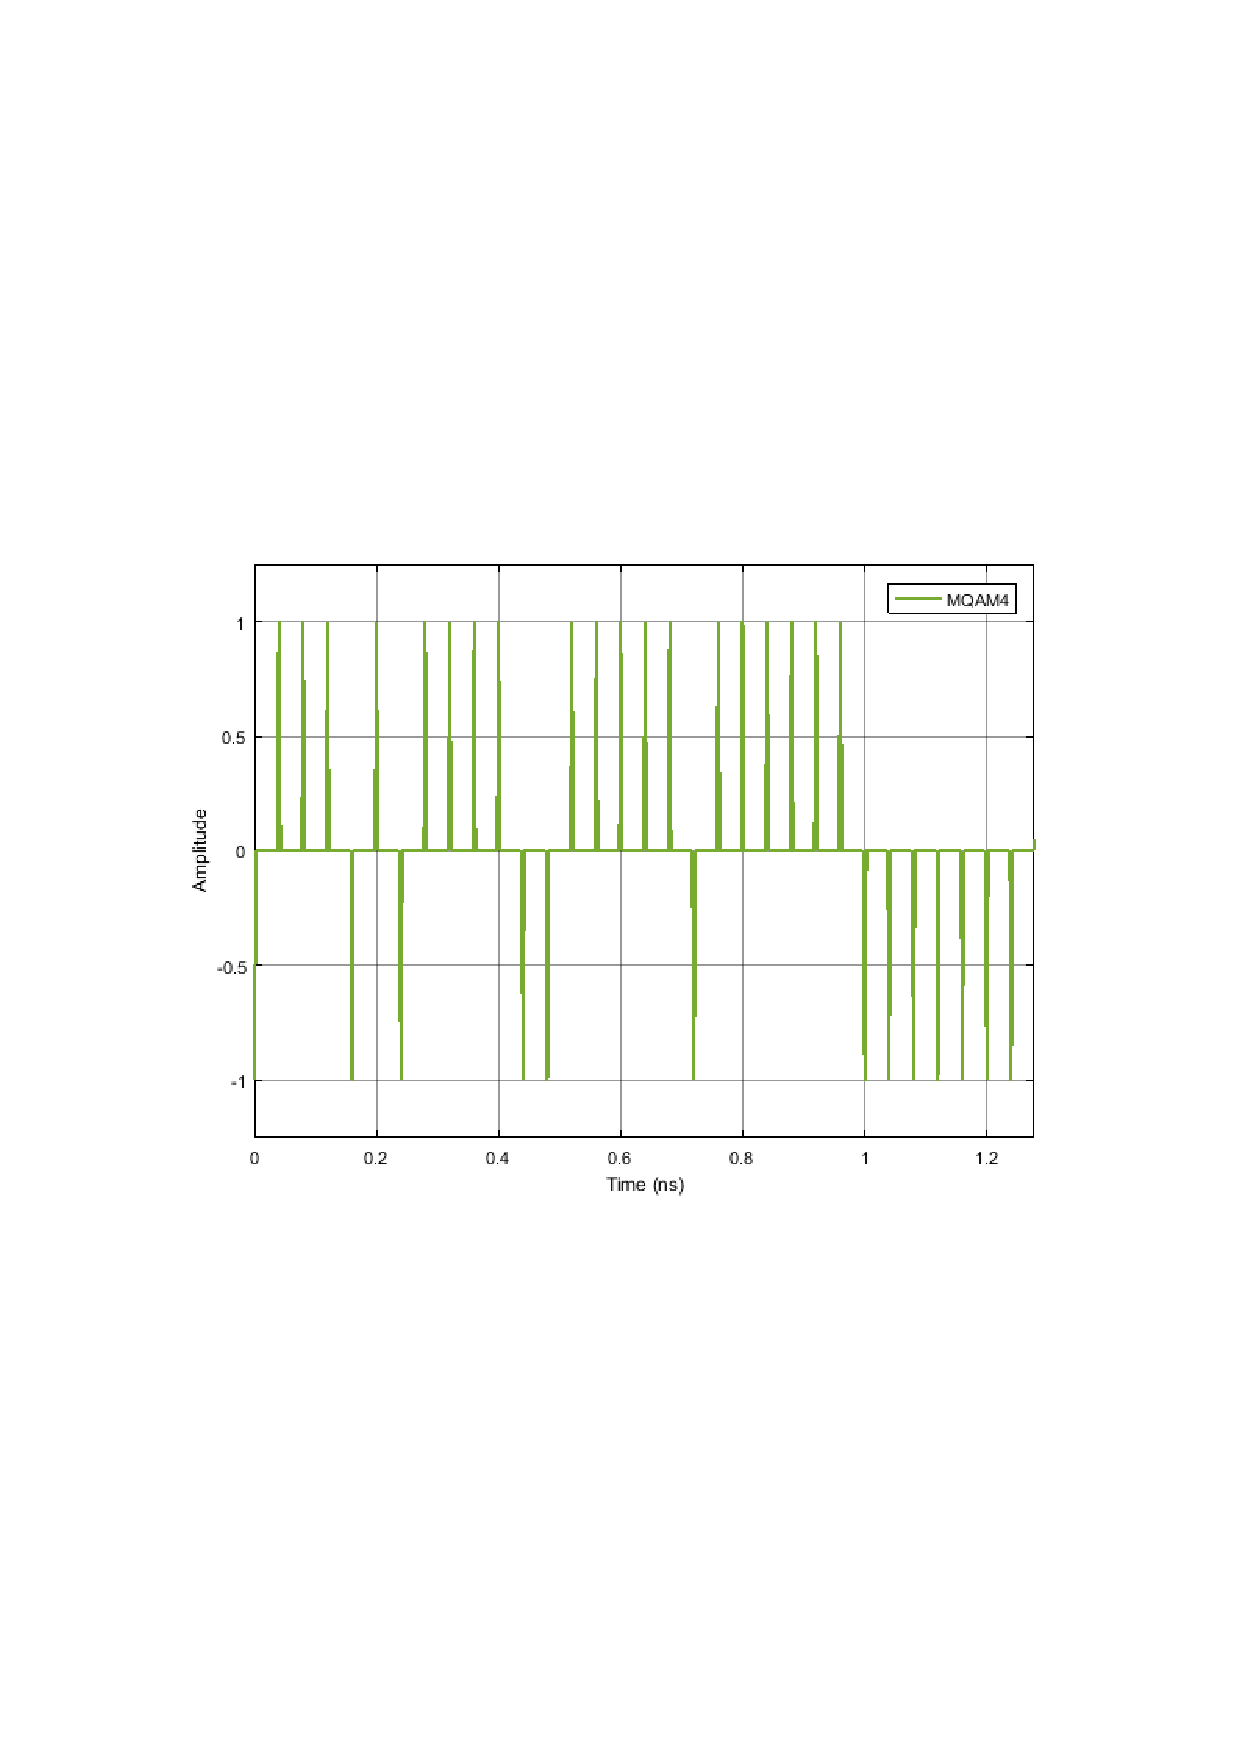
\includegraphics[clip, trim=0.5cm 9cm 0.5cm 9cm, width=\textwidth]{./lib/discrete_to_continuous_time/figures/MQAM_discrete_to_continuous_time_output.pdf}
	\label{MQAM4_DeterministicAppendZeros}\caption{Example of the type of signal generated by this block for a binary sequence 0100...}
\end{figure}

%\subsection*{Sugestions for future improvement}

\pagebreak

\clearpage

\section{DSP}

\begin{tcolorbox}	
	\begin{tabular}{p{2.75cm} p{0.2cm} p{10.5cm}} 	
		\textbf{Header File}   &:& dsp$\_*$.h \\
		\textbf{Source File}   &:& dsp$\_*$.cpp \\
        \textbf{Version}       &:& 20180423 (Celestino Martins) \\
	\end{tabular}
\end{tcolorbox}

This super block simulates the digital signal processing (DSP) algorithms for system impairments compensation in digital domain. It includes the real to complex block and carrier phase recovery block (CPE). It receives two real input signal and outputs a complex signal.

\subsection*{Input Parameters}

\begin{table}[h]
	\centering
	\begin{tabular}{|c|c|c|c|cccc}
		\cline{1-4}
		\textbf{Parameter} & \textbf{Type} & \textbf{Values} &   \textbf{Default}& \\ \cline{1-4}
		nTaps              & int & any & $25$ \\ \cline{1-4}
        NtestPhase         & int & any & $32$ \\ \cline{1-4}
        methodType         & int & any & $[0,1]$ \\ \cline{1-4}
		samplingPeriod     & double & any & $0.0$ \\ \cline{1-4}	
	\end{tabular}
	\caption{DSP input parameters}
	\label{table:dsp_in_par}
\end{table}

\subsection*{Methods}

DSP(vector$<$Signal *$>$ \&InputSig, vector$<$Signal *$>$ \&OutputSig);
\bigbreak
void setCPEnTaps(double nTaps) { B02.setnTaps(nTaps); }
\bigbreak
void setCPETestPhase(double TestPhase) { B02.setTestPhase(TestPhase); }
\bigbreak
void setCPESamplingPeriod(double sPeriod) { B02.setSamplingPeriod(sPeriod); }
\bigbreak
void setCPEmethodType(string mType) { B02.setmethodType(mType); }
\bigbreak
void setSamplingPeriod(double sPeriod) { B02.setSamplingPeriod(sPeriod); };

\subsection*{Functional description}

This super block is composed of two blocks, real to complex block and carrier phase recovery block. The two real input signals are combined into a complex signal using real to complex block. The obtained complex signal is then fed to the CPE block, where the laser phase noise compensation is performed.


\pagebreak
\subsection*{Input Signals}

\subparagraph*{Number:} 2

\subsection*{Output Signals}

\subparagraph*{Number:} 1

\subparagraph*{Type:} Electrical complex signal

\subsection*{Examples}

\subsection*{Sugestions for future improvement}



\clearpage

\section{Electrical Signal Generator}

\maketitle
This block generates time continuous amplitude continuous signal, having only one output and no input signal.

\subsection{ContinuousWave}
Continuous Wave the function of the desired signal. This must be introduce by using the function \textit{setFunction(ContinuousWave)}. This function generates a continuous signal with value 1. However, this value can be multiplied by a specific gain, which can be set by using the function \textit{setGain()}. This way, this block outputs a continuous signal with value $1 \times \textrm{gain}$.

\subsection*{Input Parameters}

	\begin{itemize}
		\item ElectricalSignalFunction signalFunction{}\linebreak
		(ContinuousWave)
		\item samplingPeriod\{\}\linebreak
        (double)
		\item symbolPeriod\{\} \linebreak
        (double)
		
	\end{itemize}

\subsection*{Methods}

ElectricalSignalGenerator() \{\};
\bigbreak	
void initialize(void);
\bigbreak	
bool runBlock(void);
\bigbreak	
void setFunction(ElectricalSignalFunction fun)
ElectricalSignalFunction getFunction()
\bigbreak	
void setSamplingPeriod(double speriod)
double getSamplingPeriod()
\bigbreak
void setSymbolPeriod(double speriod)
double getSymbolPeriod()

\bigbreak	
void setGain(double gvalue) 
double getGain() 


\subsection*{Functional description}

The \textit{signalFunction} parameter allows the user to select the signal function that the user wants to output.

\subparagraph*{Continuous Wave}
Outputs a time continuous amplitude continuous signal with amplitude 1 multiplied by the gain inserted.


\subsection*{Input Signals}

\subparagraph*{Number:} 0

\subparagraph*{Type:}No type

\subsection*{Output Signals}

\subparagraph*{Number:} 1 

\subparagraph*{Type:} TimeContinuousAmplitudeContinuous

\subsection*{Examples}


\subsection*{Sugestions for future improvement}

Implement other functions according to the needs.


\clearpage

\section{Fork}

\begin{tcolorbox}	
\begin{tabular}{p{2.75cm} p{0.2cm} p{10.5cm}} 	
\textbf{Header File}   &:& fork\_20171119.h \\
\textbf{Source File}   &:& fork\_20171119.cpp \\
\textbf{Version}       &:& 20171119 (\textbf{Student Name}: Romil Patel)
\end{tabular}
\end{tcolorbox}

\subsection*{Input Parameters}

--- NA ---

\subsection*{Input Signals}

\textbf{Number}: 1\\
\textbf{Type}: Any type (BinaryValue, IntegerValue, RealValue, ComplexValue, ComplexValueXY, PhotonValue, PhotonValueMP, Message)

\subsection*{Output Signals}

\textbf{Number}: 2\\
\textbf{Type}: Same as applied to the input.\\
\\
\textbf{Number}: 3\\
\textbf{Type}: Same as applied to the input.

\subsection*{Functional Description}

This block accepts any type signal and outputs two replicas of the input signal.

\begin{figure}[h]
	\centering
	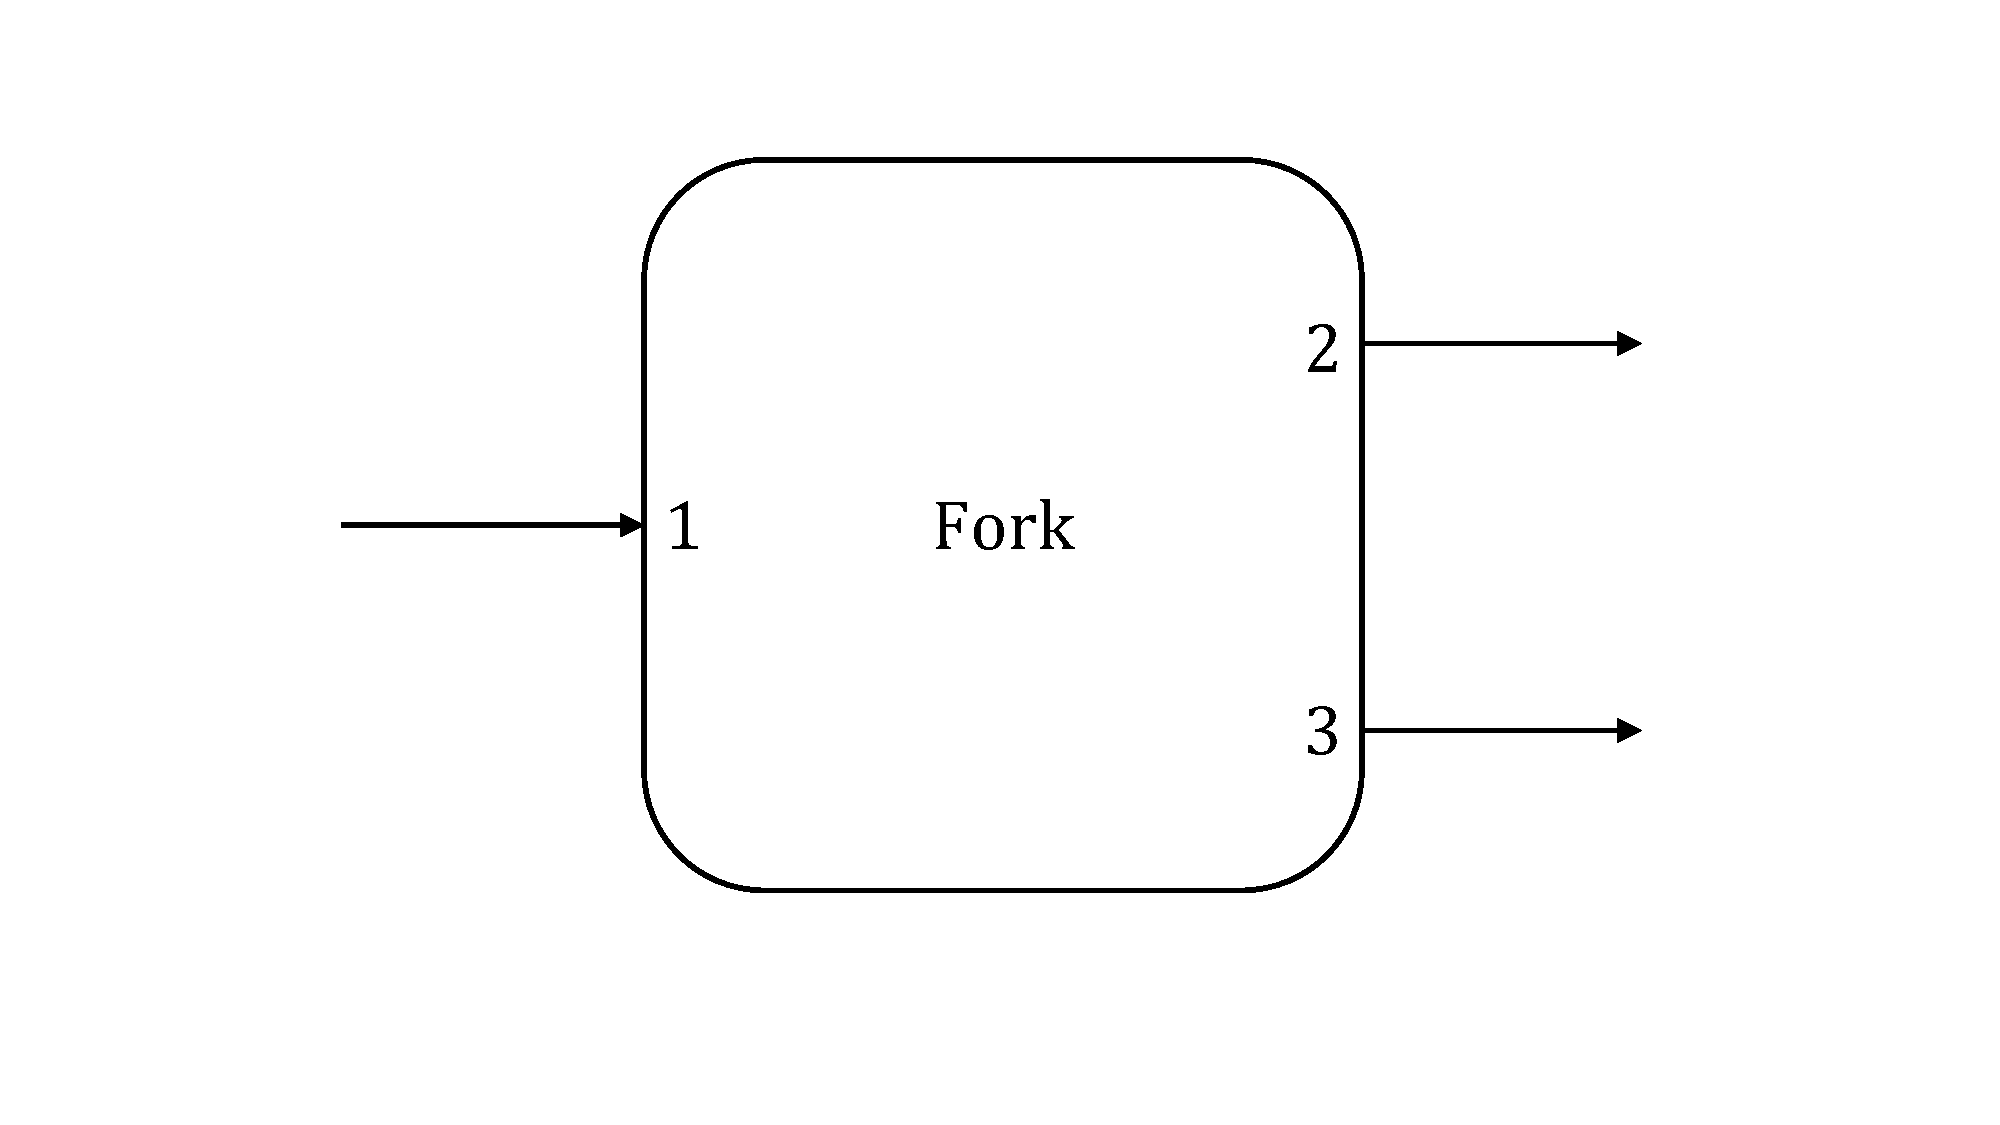
\includegraphics[width=0.6\textwidth, height=4.5cm]{./lib/fork/figures/fork.pdf}
	\caption{Fork}\label{}
\end{figure}
\clearpage

\section{Gaussian Source}

\begin{tcolorbox}	
	\begin{tabular}{p{2.75cm} p{0.2cm} p{10.5cm}} 	
		\textbf{Header File}   &:& gaussian\_source.h \\
		\textbf{Source File}   &:& gaussian\_source.cpp \\
	\end{tabular}
\end{tcolorbox}

This block simulates a random number generator that follows a Gaussian statistics. It produces one output real signal and it doesn't accept input signals.

\subsection*{Input Parameters}

\begin{table}[h]
	\centering
	\begin{tabular}{|c|c|c|c|cccc}
		\cline{1-4}
		\textbf{Parameter} & \textbf{Type} & \textbf{Values} &   \textbf{Default}& \\ \cline{1-4}
		mean & double & any & $0$ \\ \cline{1-4}
		Variance & double & any & $1$ \\ \cline{1-4}
	\end{tabular}
	\caption{Gaussian source input parameters}
	\label{table_Gaussian_Source}
\end{table}


\subsection*{Methods}

GaussianSource() {}
\bigbreak
GaussianSource(vector$<$Signal *$>$ \&InputSig, vector$<$Signal *$>$ \&OutputSig) :Block(InputSig, OutputSig)\{\};
\bigbreak
void initialize(void);
\bigbreak
bool runBlock(void);
\bigbreak
void setAverage(double Average) ;

\subsection*{Functional description}

This block generates a complex signal with a specified phase given by the input parameter \textit{phase}.

\pagebreak
\subsection*{Input Signals}

\subparagraph*{Number:} 0

\subsection*{Output Signals}

\subparagraph*{Number:} 1

\subparagraph*{Type:} Continuous signal (TimeDiscreteAmplitudeContinuousReal)

\subsection*{Examples}

\subsection*{Sugestions for future improvement}



\clearpage

\section{MQAM Receiver}

\begin{tcolorbox}	
	\begin{tabular}{p{2.75cm} p{0.2cm} p{10.5cm}} 	
		\textbf{Header File}   &:& m\_qam\_receiver.h \\
		\textbf{Source File}   &:& m\_qam\_receiver.cpp \\
	\end{tabular}
\end{tcolorbox}

\paragraph{Warning:}\textit{homodyne\_receiver} is not recommended. Use \textit{m\_qam\_homodyne\_receiver} instead.
\newline

This block of code simulates the reception and demodulation of an optical signal (which is the input signal of the system) outputing a binary signal. A simplified schematic representation of this block is shown in figure \ref{MQAM_receiver_block_diagram_simple}.

\begin{figure}[h]
	\centering
	\includegraphics[width=0.8\textwidth]{../lib/homodyne_receiver/figures/MQAM_receiver_block_diagram_simple}
	\caption{Basic configuration of the MQAM receiver}\label{MQAM_receiver_block_diagram_simple}
\end{figure}

\subsection*{Functional description}

This block accepts one optical input signal and outputs one binary signal that corresponds to the M-QAM demodulation of the input signal. It is a complex block (as it can be seen from figure \ref{MQAM_receiver_block_diagram}) of code made up of several simpler blocks whose description can be found in the \textit{lib} repository.

In can also be seen from figure \ref{MQAM_receiver_block_diagram} that there's an extra internal (generated inside the homodyne receiver block) input signal generated by the \textit{Clock}. This block is used to provide the sampling frequency to the \textit{Sampler}.


\begin{figure}[h]
	\centering
	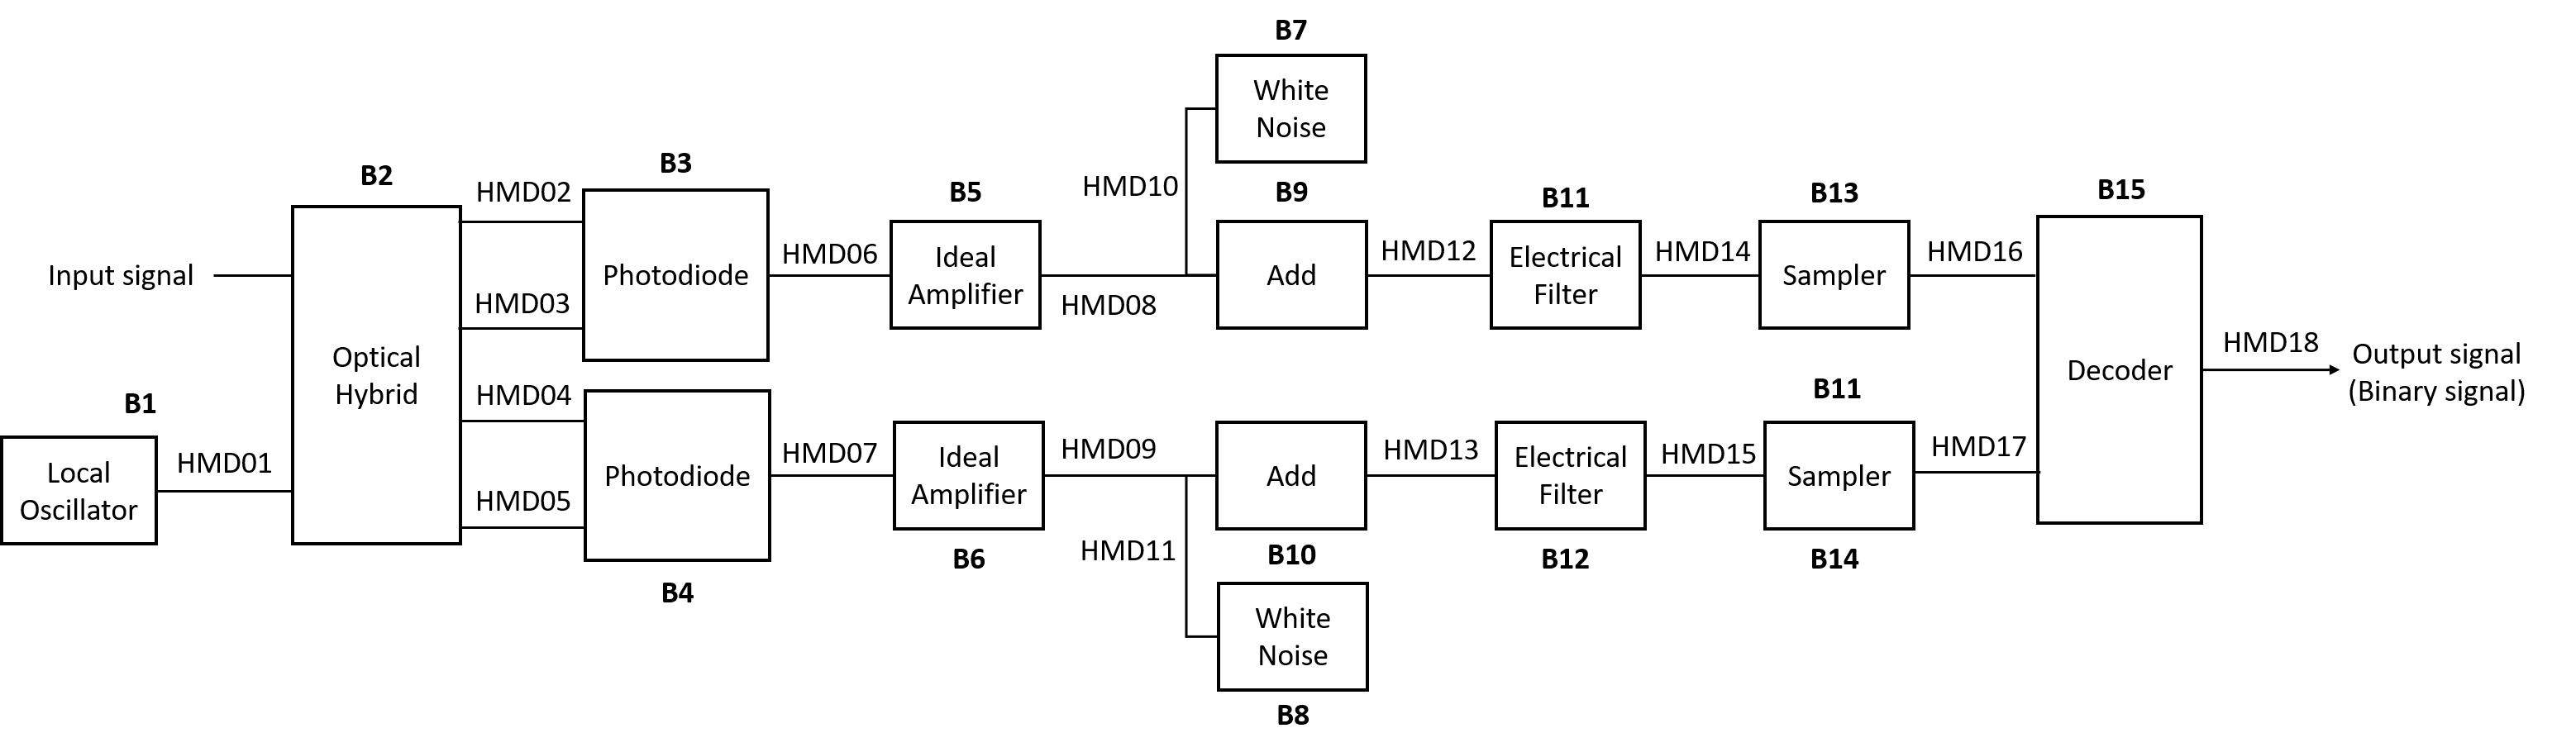
\includegraphics[width=\textwidth]{../lib/homodyne_receiver/figures/MQAM_receiver_block_diagram_20180206.png}
	\caption{Schematic representation of the block homodyne receiver.}\label{MQAM_receiver_block_diagram}
\end{figure}

\subsection*{Input parameters}

This block has some input parameters that can be manipulated by the user in order oto change the basic configuration of the receiver. Each parameter has associated a function that allows for its change. In the following table (table~\ref{table}) the input parameters and corresponding functions are summarized.

\begin{table}[h]
	\begin{center}
		\begin{tabular}{| m{3,2cm} | m{6,2cm} |  m{2,2cm} | m{4cm} | }
			\hline
			\textbf{Input parameters} & \textbf{Function} & \textbf{Type} & \textbf{Accepted values} \\ \hline
			IQ amplitudes & setIqAmplitudes & Vector of coordinate points in the I-Q plane & \textbf{Example} for a 4-QAM mapping: \{ \{ 1.0, 1.0 \}, \{ -1.0, 1.0 \}, \{ -1.0, -1.0 \}, \{ 1.0, -1.0 \} \} \\ \hline
			Local oscillator power (in dBm) & setLocalOscillatorOpticalPower\_dBm & double(t\_real) & Any double greater than zero\\ \hline
			Local oscillator phase & setLocalOscillatorPhase & double(t\_real) & Any double greater than zero\\ \hline
			Responsivity of the photodiodes & setResponsivity & double(t\_real) &$\in$ [0,1] \\ \hline
			Amplification (of the TI amplifier) & setAmplification & double(t\_real) & Positive real number\\ \hline
			Noise amplitude (introduced by the TI amplifier) & setNoiseAmplitude & double(t\_real) & Real number greater than zero \\ \hline
			Samples to skipe & setSamplesToSkip & int(t\_integer) &  \\ \hline
			Save internal signals & setSaveInternalSignals & bool & True or False\\ \hline
			Sampling period & setSamplingPeriod & double & Given by \textit{symbolPeriod}/\textit{samplesPerSymbol}\\
			\hline
		\end{tabular}
		\caption{List of input parameters of the block MQAM receiver} \label{table}
	\end{center}
\end{table}

\pagebreak

\subsection*{Methods}

HomodyneReceiver(vector$<$Signal *$>$ \&inputSignal, vector$<$Signal *$>$ \&outputSignal) (\textbf{constructor})
\bigbreak
void setIqAmplitudes(vector$<$t\_iqValues$>$ iqAmplitudesValues)
\bigbreak
vector$<$t\_iqValues$>$ const getIqAmplitudes(void)
\bigbreak
void setLocalOscillatorSamplingPeriod(double sPeriod)
\bigbreak
void setLocalOscillatorOpticalPower(double opticalPower)
\bigbreak
void setLocalOscillatorOpticalPower\_dBm(double opticalPower\_dBm)
\bigbreak
void setLocalOscillatorPhase(double lOscillatorPhase)
\bigbreak
void setLocalOscillatorOpticalWavelength(double lOscillatorWavelength)
\bigbreak
void setSamplingPeriod(double sPeriod)
\bigbreak
void  setResponsivity(t\_real Responsivity)
\bigbreak
void setAmplification(t\_real Amplification)
\bigbreak
void setNoiseAmplitude(t\_real NoiseAmplitude)
\bigbreak
void setImpulseResponseTimeLength(int impResponseTimeLength)
\bigbreak
void setFilterType(PulseShaperFilter fType)
\bigbreak
void setRollOffFactor(double rOffFactor)
\bigbreak
void setClockPeriod(double per)
\bigbreak
void setSamplesToSkip(int sToSkip)

\pagebreak

\subsection*{Input Signals}

\subparagraph*{Number:} 1

\subparagraph*{Type:} Optical signal

\subsection*{Output Signals}

\subparagraph*{Number:} 1

\subparagraph*{Type:} Binary signal

\subsection*{Example}

\subsection*{Sugestions for future improvement}

\clearpage

\section{IQ Modulator}

\begin{tcolorbox}	
	\begin{tabular}{p{2.75cm} p{0.2cm} p{10.5cm}} 	
		\textbf{Header File}   &:& iq\_modulator.h \\
		\textbf{Source File}   &:& iq\_modulator.cpp \\
	\end{tabular}
\end{tcolorbox}

This blocks accepts one inupt signal continuous in both time and amplitude and it can produce either one or two output signals. It generates an optical signal and it can also generate a binary signal.

\subsection*{Input Parameters}

\begin{table}[h]
	\centering
	\begin{tabular}{|c|c|c|c|cccc}
		\cline{1-4}
		\textbf{Parameter} & \textbf{Type} & \textbf{Values} &   \textbf{Default}& \\ \cline{1-4}
		outputOpticalPower & double & any & $1e-3$ \\ \cline{1-4}
		outputOpticalWavelength & double & any & $1550e-9$ \\ \cline{1-4}
		outputOpticalFrequency & double & any & speed\_of\_light/outputOpticalWavelength \\ \cline{1-4}
	\end{tabular}
	\caption{Binary source input parameters}
	\label{table:iqmod_in_par}
\end{table}

%\begin{itemize}
%	\item outputOpticalPower\{1e-3\} \linebreak
%	(double)
%	\item outputOpticalWavelength\{1550e-9\} \linebreak (double)
%	\item outputOpticalFrequency\{speed$\_$of$\_$light/outputOpticalWavelength\} \linebreak
%	(double)
%\end{itemize}

\subsection*{Methods}

IqModulator(vector$<$Signal *$>$ \&InputSig, vector$<$Signal *$>$ \&OutputSig) :Block(InputSig, OutputSig)\{\};
\bigbreak
void initialize(void);
\bigbreak
bool runBlock(void);
\bigbreak
void setOutputOpticalPower(double outOpticalPower)
\bigbreak
void setOutputOpticalPower$\_$dBm(double outOpticalPower$\_$dBm)
\bigbreak
void setOutputOpticalWavelength(double outOpticalWavelength)
\bigbreak
void setOutputOpticalFrequency(double outOpticalFrequency)

\subsection*{Functional Description}

This block takes the two parts of the signal: in phase and in amplitude and it combines them to produce a complex signal that contains information about the amplitude and the phase.

This complex signal is multiplied by $\frac{1}{2}\sqrt{\textit{outputOpticalPower}}$ in order to reintroduce the information about the energy (or power) of the signal. This signal corresponds to an optical signal and it can be a scalar or have two polarizations along perpendicular axis. It is the signal that is transmited to the receptor.

The binary signal is sent to the Bit Error Rate (BER) meaurement block.

\subsection*{Input Signals}

\subparagraph*{Number}: 2

\subparagraph*{Type}: Sequence of impulses modulated by the filter (ContinuousTimeContiousAmplitude))

\subsection*{Output Signals}

\subparagraph*{Number}: 1 or 2

\subparagraph*{Type}: Complex signal (optical) (ContinuousTimeContinuousAmplitude) and binary signal (DiscreteTimeDiscreteAmplitude)

\subsection*{Example}
\begin{figure}[h]
	\centering
	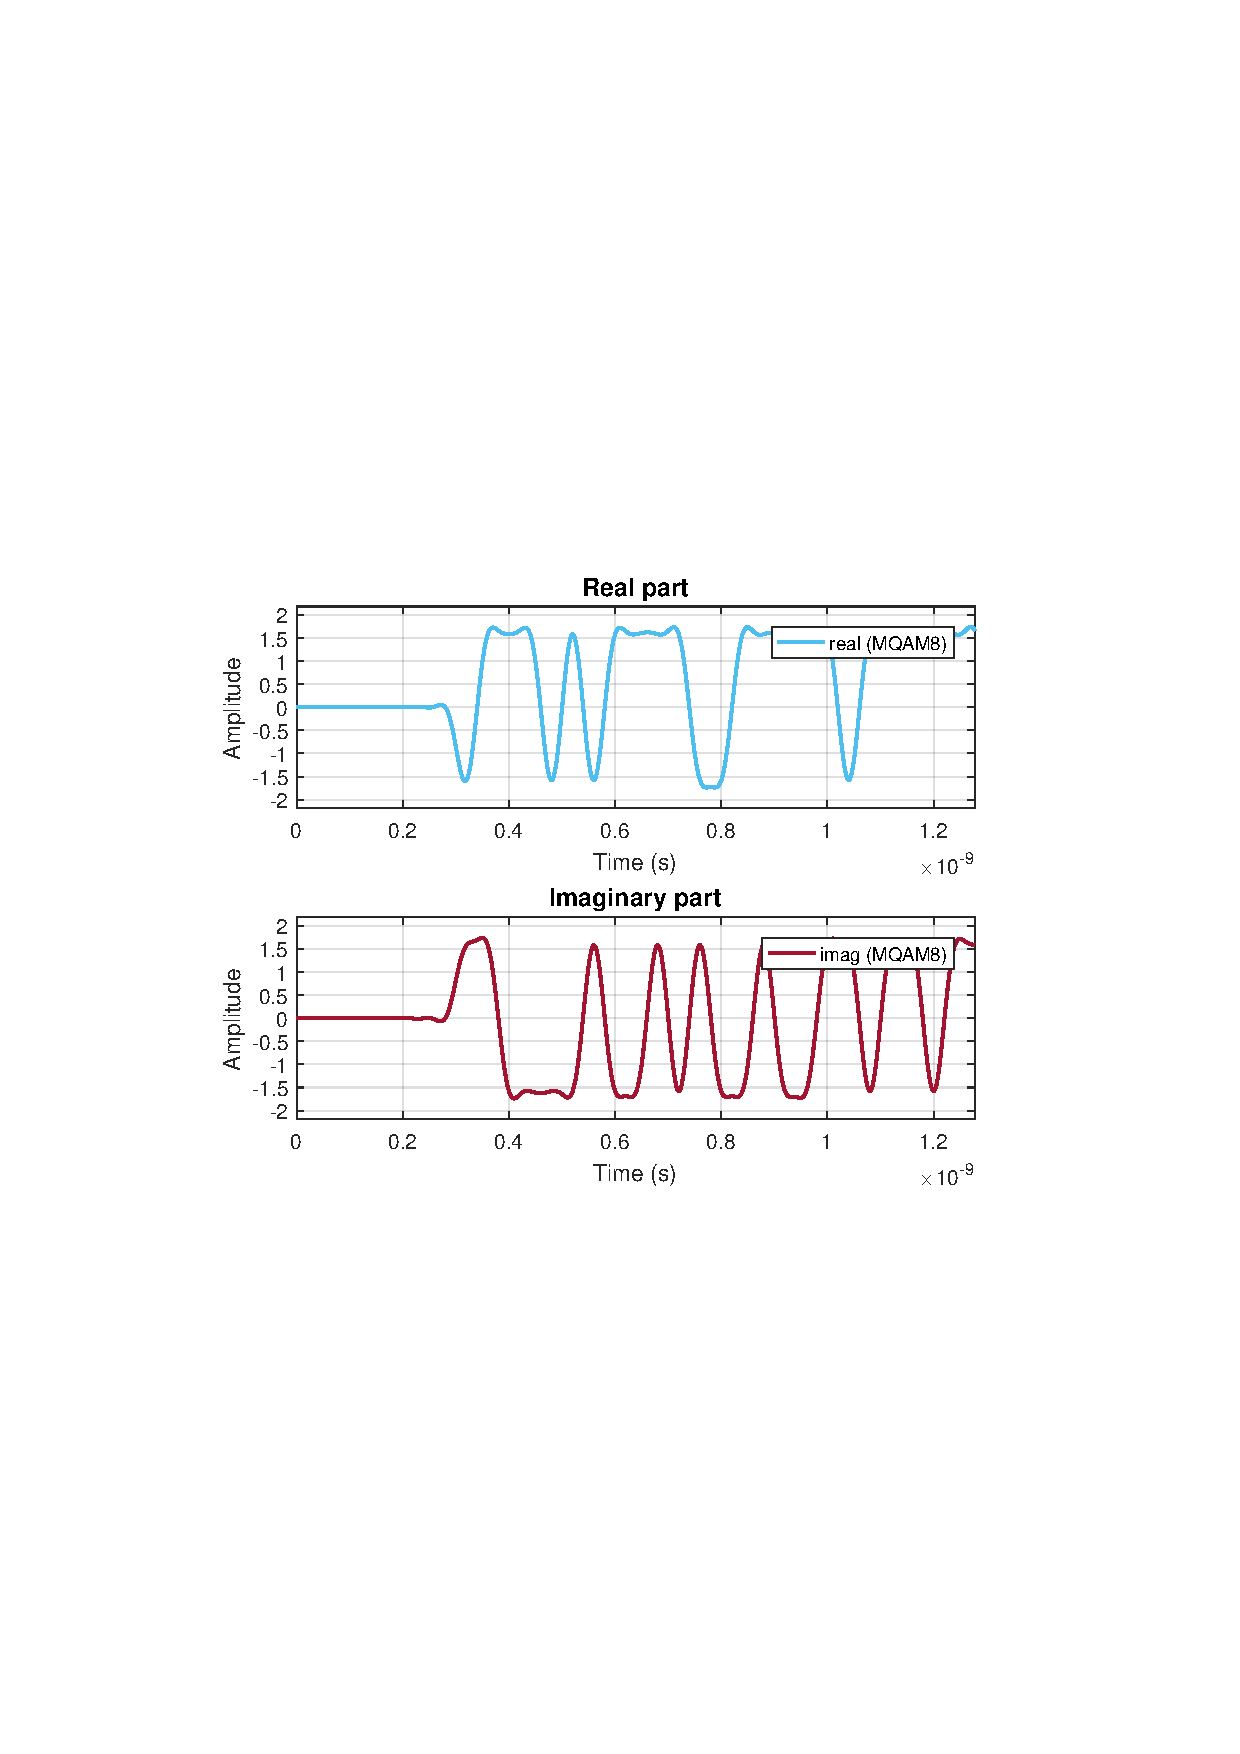
\includegraphics[clip, trim=0.5cm 9cm 0.5cm 9cm, width=\textwidth]{./lib/iq_modulator/figures/MQAM_iq_modulator_output.pdf}
	\label{MQAM8_DeterministicAppendZeros}\caption{Example of a signal generated by this block for the initial binary signal 0100...}
\end{figure}

%\subsection*{Sugestions for future improvement}

\clearpage

\section{Local Oscillator}

\begin{tcolorbox}	
	\begin{tabular}{p{2.75cm} p{0.2cm} p{10.5cm}} 	
		\textbf{Header File}   &:& local\_oscillator.h \\
		\textbf{Source File}   &:& local\_oscillator.cpp \\
        \textbf{Version}       &:& 20180130
	\end{tabular}
\end{tcolorbox}

This block simulates a local oscillator with constant power and initial phase. It produces one output complex signal and it doesn't accept input signals.

\subsection*{Input Parameters}

\begin{table}[h]
	\centering
	\begin{tabular}{|c|c|c|c|cccc}
		\cline{1-4}
		\textbf{Parameter} & \textbf{Type} & \textbf{Values} &   \textbf{Default}& \\ \cline{1-4}
		opticalPower & double & any & $1\text{e}-3$ \\ \cline{1-4}
		outputOpticalWavelength & double & any & $1550\text{e}-9$ \\ \cline{1-4}
		outputOpticalFrequency & double & any &  SPEED\_OF\_LIGHT / outputOpticalWavelength \\ \cline{1-4}
		phase & double & $\in \left[0,\frac{\pi}{2}\right]$ & $0$ \\ \cline{1-4}
		samplingPeriod & double & any & $0.0$ \\ \cline{1-4}
        symbolPeriod   & double & any & $0.0$ \\ \cline{1-4}
        signaltoNoiseRatio & double & any & $0.0$ \\ \cline{1-4}
        laserLineWidth & double & any & $0.0$ \\ \cline{1-4}
        laserRIN       & double & any & $0.0$ \\ \cline{1-4}
	\end{tabular}
	\caption{Binary source input parameters}
	\label{table:LO_in_par}
\end{table}

%
%\begin{itemize}
%	\item opticalPower\{ 1e-3 \}
%	\item wavelength\{ 1550e-9 \}
%	\item frequency\{ SPEED\_OF\_LIGHT / wavelength \}
%	\item phase\{ 0 \}
%	\item samplingPeriod\{ 0.0 \}
%\end{itemize}

\subsection*{Methods}

LocalOscillator() {}
\bigbreak
LocalOscillator(vector$<$Signal *$>$ \&InputSig, vector$<$Signal *$>$ \&OutputSig) :Block(InputSig, OutputSig)\{\};
\bigbreak
void initialize(void);
\bigbreak
bool runBlock(void);
\bigbreak
void setSamplingPeriod(double sPeriod);
\bigbreak
void setSymbolPeriod(double sPeriod);
\bigbreak
void setOpticalPower(double oPower);
\bigbreak
void setOpticalPower\_dBm(double oPower\_dBm);
\bigbreak
void setWavelength(double wlength);
\bigbreak
void setFrequency(double freq);
\bigbreak
void setPhase(double lOscillatorPhase);
\bigbreak
void setSignaltoNoiseRatio(double sNoiseRatio);
\bigbreak
void setLaserLinewidth(double laserLinewidth);
\bigbreak
void setLaserRIN(double laserRIN);

\subsection*{Functional description}

This block generates a complex signal with a specified phase given by the input parameter \textit{phase}.

\subsection*{Input Signals}

\textbf{Number:} 0

\subsection*{Output Signals}

\textbf{Number:} 1\\
\textbf{Type:} Optical signal


\clearpage

\section{Local Oscillator}

\begin{tcolorbox}	
	\begin{tabular}{p{2.75cm} p{0.2cm} p{10.5cm}} 	
		\textbf{Header File}   &:& local\_oscillator.h \\
		\textbf{Source File}   &:& local\_oscillator.cpp \\
	\end{tabular}
\end{tcolorbox}

This block simulates a local oscillator with constant power and initial phase. It produces one output complex signal and it doesn't accept input signals.

\subsection*{Input Parameters}

\begin{table}[h]
	\centering
	\begin{tabular}{|c|c|c|c|cccc}
		\cline{1-4}
		\textbf{Parameter} & \textbf{Type} & \textbf{Values} &   \textbf{Default}& \\ \cline{1-4}
		opticalPower & double & any & $1\text{e}-3$ \\ \cline{1-4}
		outputOpticalWavelength & double & any & $1550\text{e}-9$ \\ \cline{1-4}
		outputOpticalFrequency & double & any &  SPEED\_OF\_LIGHT / outputOpticalWavelength \\ \cline{1-4}
		phase0 & double & $\in \left[0,\frac{\pi}{2}\right]$ & $0$ \\ \cline{1-4}
		samplingPeriod & double & any & $0.0$ \\ \cline{1-4}
        laserLW & double & any & $0.0$ \\ \cline{1-4}
        laserRIN & double & any & $0.0$ \\ \cline{1-4}
	\end{tabular}
	\caption{Local oscillator input parameters}
	\label{table:LO_in_par}
\end{table}

%
%\begin{itemize}
%	\item opticalPower\{ 1e-3 \}
%	\item wavelength\{ 1550e-9 \}
%	\item frequency\{ SPEED\_OF\_LIGHT / wavelength \}
%	\item phase\{ 0 \}
%	\item samplingPeriod\{ 0.0 \}
%\end{itemize}

\subsection*{Methods}

LocalOscillator() {}
\bigbreak
LocalOscillator(vector$<$Signal *$>$ \&InputSig, vector$<$Signal *$>$ \&OutputSig) :Block(InputSig, OutputSig)\{\};
\bigbreak
void initialize(void);
\bigbreak
bool runBlock(void);
\bigbreak
void setSamplingPeriod(double sPeriod);
\bigbreak
void setOpticalPower(double oPower);
\bigbreak
void setOpticalPower\_dBm(double oPower\_dBm);
\bigbreak
void setWavelength(double wlength);
\bigbreak
void setPhase(double lOscillatorPhase);
\bigbreak
void setLaserLinewidth(double laserLinewidth);
\bigbreak
double getLaserLinewidth();
\bigbreak
void setLaserRIN(double LOlaserRIN);
\bigbreak
double getLaserRIN();

\subsection*{Functional description}

This block generates a complex signal with a specified initial phase given by the input parameter \textit{phase0}. The phase noise can be simulated by adjusting the laser linewidth in parameter \textit{laserLW}. The relative intensity noise (RIN) can be also adjusting according to the parameter \textit{laserRIN}.

\pagebreak
\subsection*{Input Signals}

\subparagraph*{Number:} 0

\subsection*{Output Signals}

\subparagraph*{Number:} 1

\subparagraph*{Type:} Optical signal

\subsection*{Examples}

\subsection*{Sugestions for future improvement}



\clearpage

\section{MQAM Mapper}

\begin{tcolorbox}	
	\begin{tabular}{p{2.75cm} p{0.2cm} p{10.5cm}} 	
		\textbf{Header File}   &:& m\_qam\_mapper.h \\
		\textbf{Source File}   &:& m\_qam\_mapper.cpp \\
	\end{tabular}
\end{tcolorbox}

This block does the mapping of the binary signal using a \textit{m}-QAM modulation. It accepts one input signal of the binary type and it produces two output signals which are a sequence of 1's and -1's.

\subsection*{Input Parameters}

\begin{table}[h]
	\centering
	\begin{tabular}{|c|c|c|p{50mm}|cccp{50mm}}
		\cline{1-4}
		\textbf{Parameter} & \textbf{Type} & \textbf{Values} &   \textbf{Default}& \\ \cline{1-4}
		m & int & $2^n$ with $n$ integer & $4$ \\ \cline{1-4}
		iqAmplitudes & vector$<$\texttt{t\_complex}$>$ & \---- & \{ \{ 1.0, 1.0 \},\{ -1.0, 1.0 \},\{ -1.0, -1.0 \},\{ 1.0, -1.0 \} \} \\ \cline{1-4}
	\end{tabular}
	\caption{Binary source input parameters}
	\label{table:mapper_in_par}
\end{table}

%\begin{itemize}
%	\item m\{4\} \linebreak
%	(m should be of the form $2^n$ with n integer)
%	\item iqAmplitudes\{\{ 1.0, 1.0 \}, \{ -1.0, 1.0 \}, \{ -1.0, -1.0 \}, \{ 1.0, -1.0 \}\} \linebreak
%	
%\end{itemize}

\subsection*{Methods}

MQamMapper(vector$<$Signal *$>$ \&InputSig, vector$<$Signal *$>$ \&OutputSig) :Block(InputSig, OutputSig) \{\};
\bigbreak	
void initialize(void);
\bigbreak	
bool runBlock(void);
\bigbreak	
void setM(int mValue);
\bigbreak	
void setIqAmplitudes(vector$<$t\_iqValues$>$ iqAmplitudesValues);

\subsection*{Functional Description}

In the case of m=4 this block atributes to each pair of bits a point in the I-Q space. The constellation used is defined by the \textit{iqAmplitudes} vector. The constellation used in this case is ilustrated in figure \ref{constellation}.

\begin{figure}
	\centering
	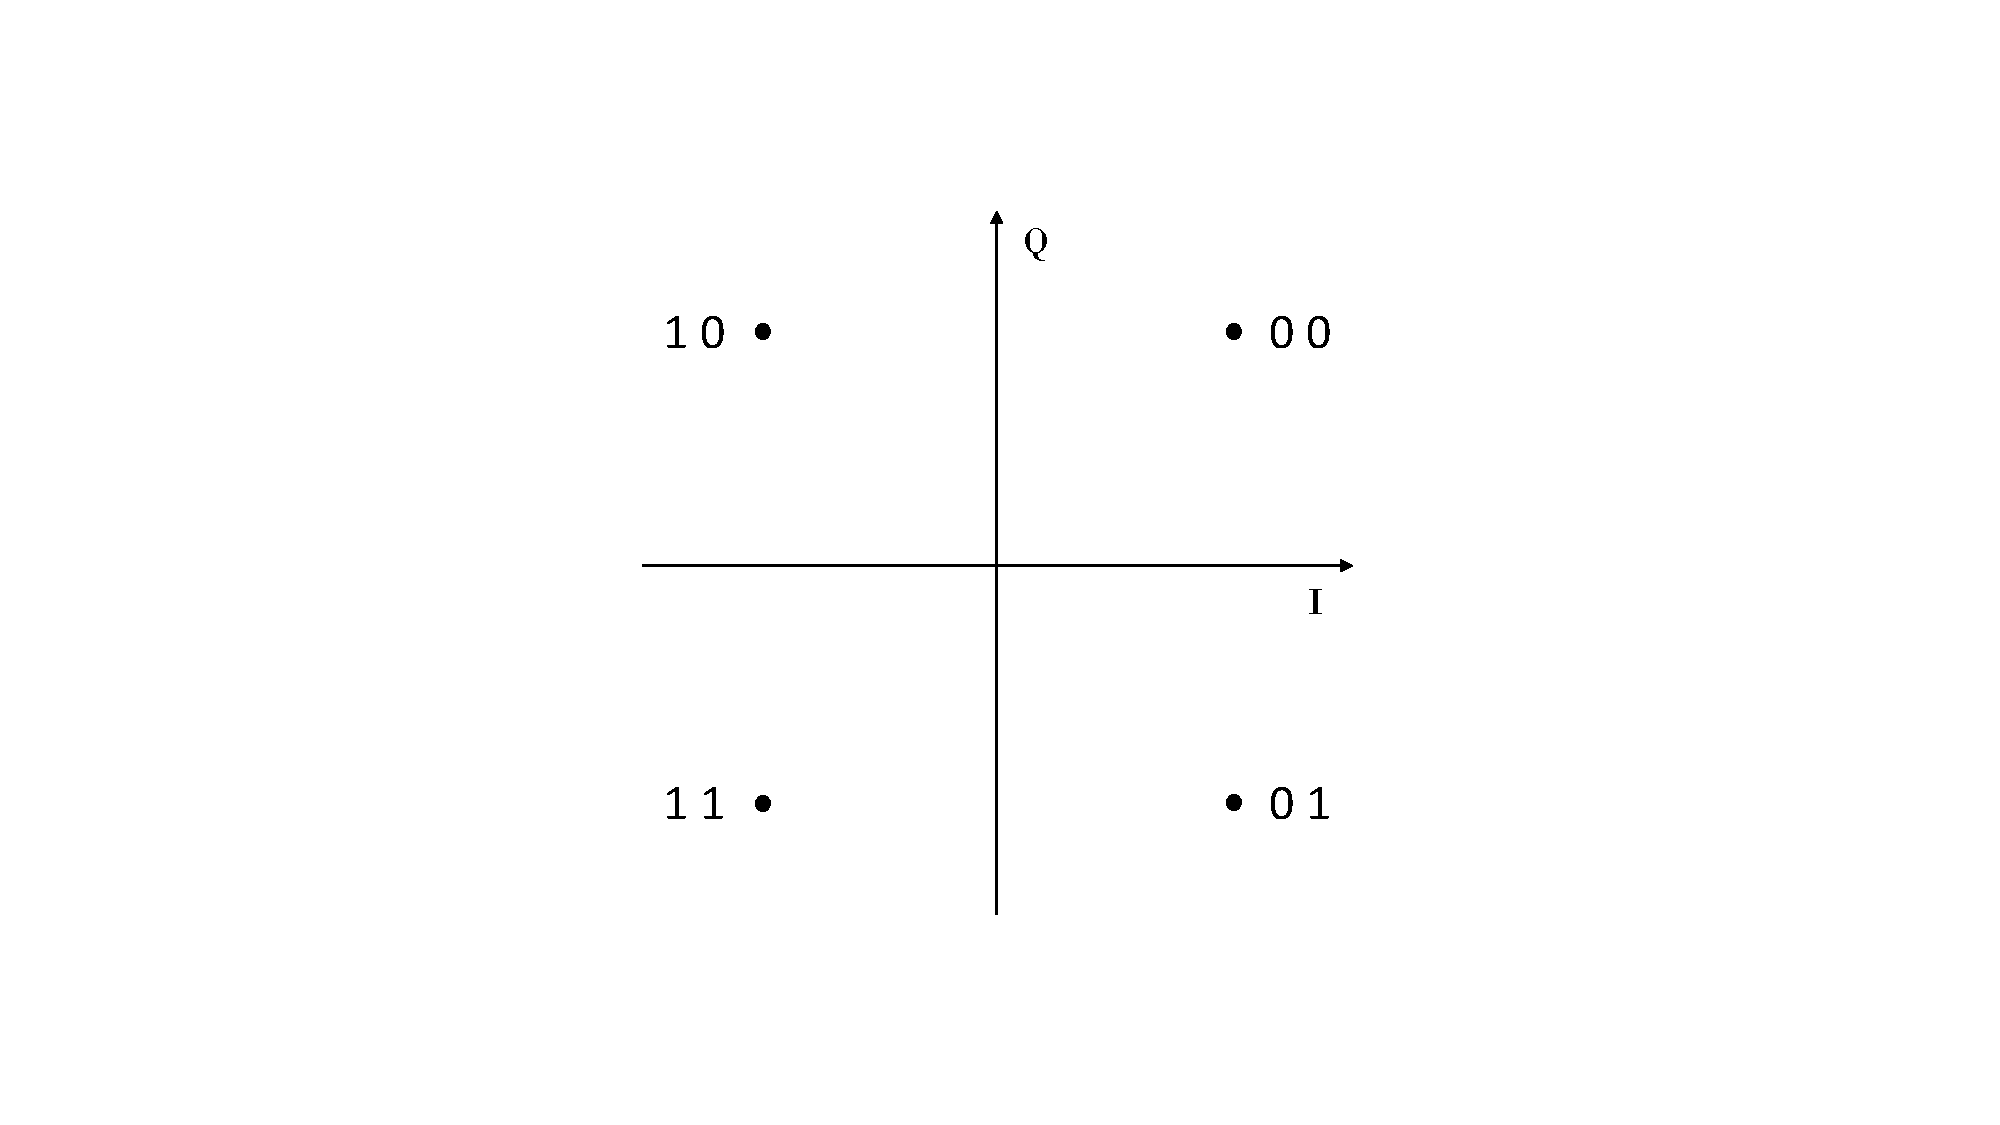
\includegraphics[width=\textwidth]{./lib/m_qam_mapper/figures/MQAM_constellation.pdf}
	
	\caption{Constellation used to map the signal for m=4 }\label{constellation}
	
\end{figure}

\subsection*{Input Signals}

\subparagraph*{Number}: 1

\subparagraph*{Type}: Binary (DiscreteTimeDiscreteAmplitude)

\subsection*{Output Signals}

\subparagraph*{Number}: 2

\subparagraph*{Type}: Sequence of 1's and -1's (DiscreteTimeDiscreteAmplitude)

\subsection*{Example}

\begin{figure}[h]
	\centering
	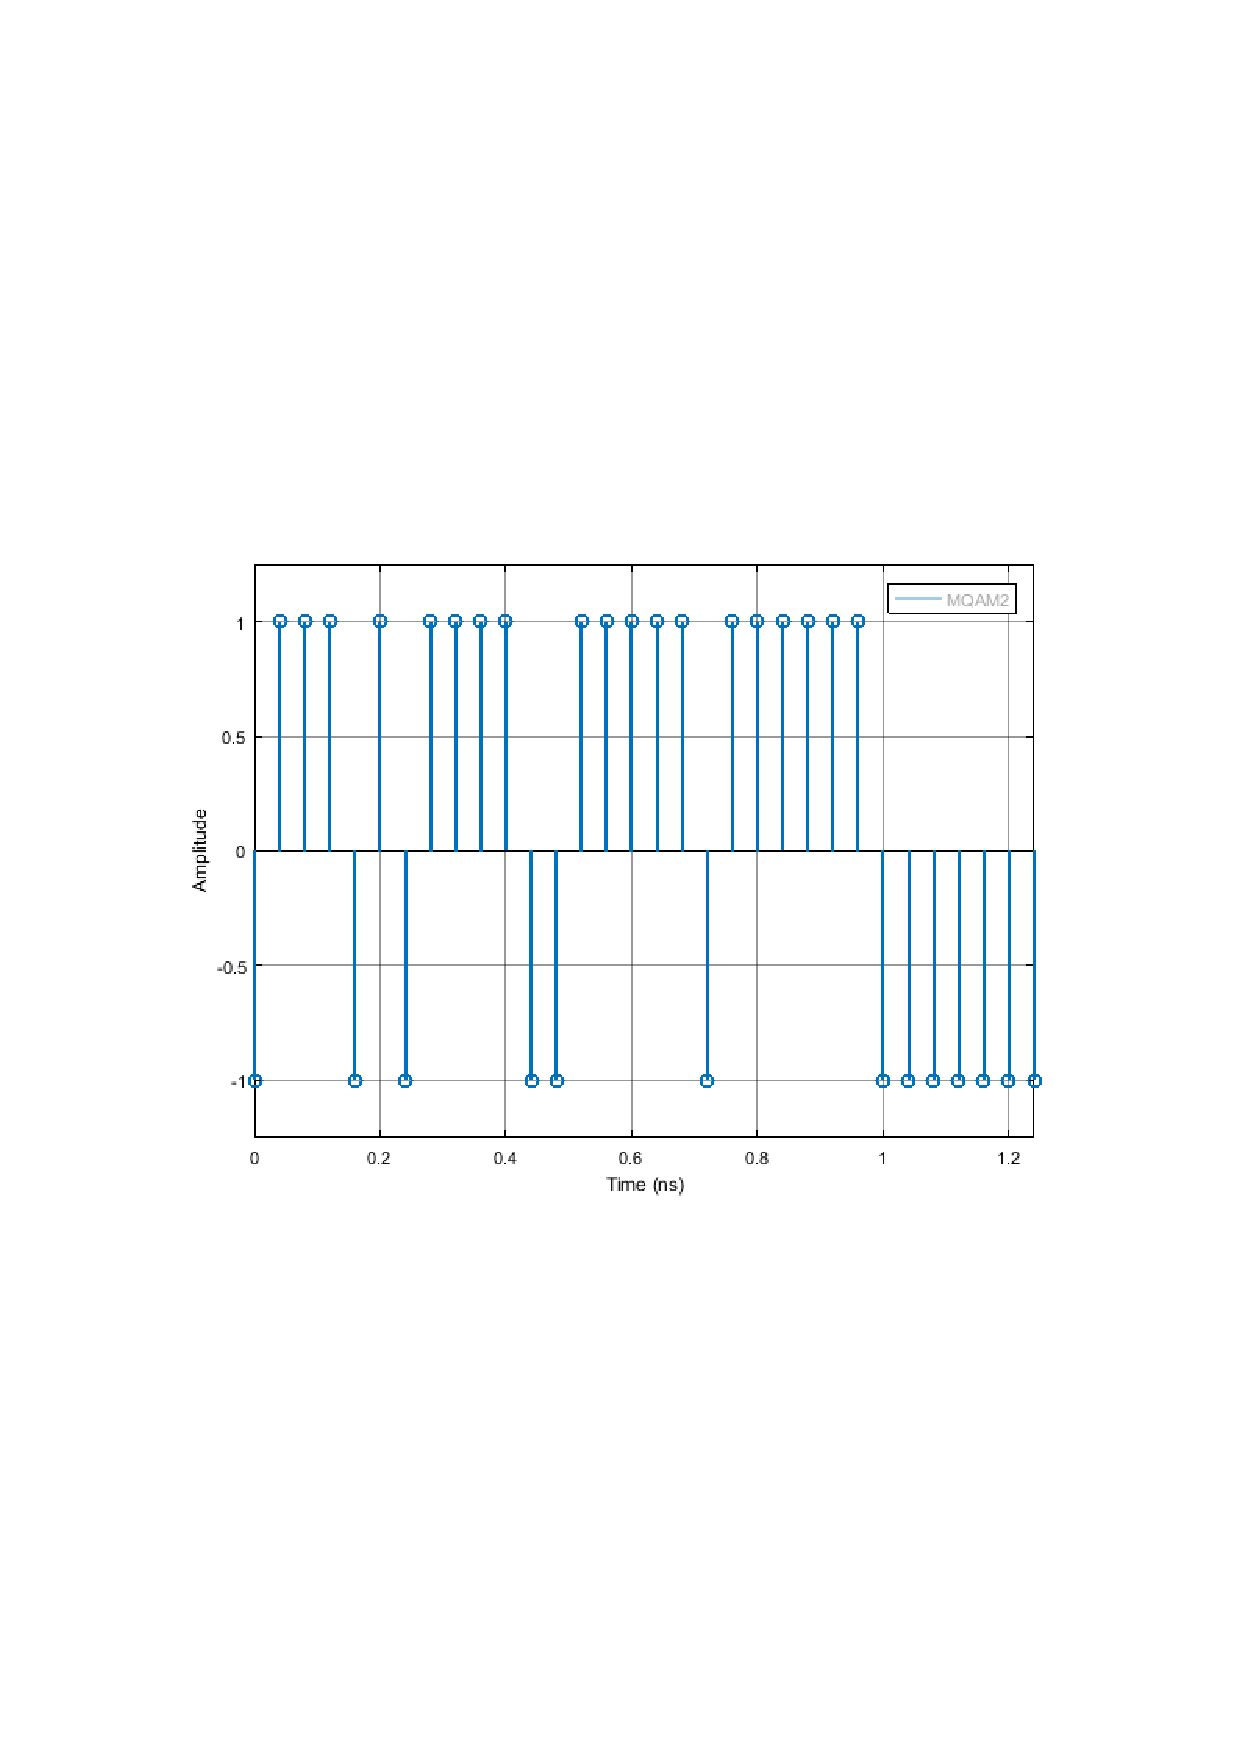
\includegraphics[clip, trim=0.5cm 9cm 0.5cm 9cm, width=\textwidth]{./lib/m_qam_mapper/figures/MQAM_mapper_output.pdf}
	
	\caption{Example of the type of signal generated by this block for the initial binary signal 0100... }\label{DeterministicAppendZeros}

\end{figure}

%\subsection*{Sugestions for future improvement}

\clearpage

\section{MQAM Transmitter}

\begin{tcolorbox}	
	\begin{tabular}{p{2.75cm} p{0.2cm} p{10.5cm}} 	
		\textbf{Header File}   &:& m\_qam\_transmitter.h \\
		\textbf{Source File}   &:& m\_qam\_transmitter.cpp \\
	\end{tabular}
\end{tcolorbox}

This block generates a MQAM optical signal. It can also output the binary sequence. A schematic representation of this block is shown in figure \ref{MQAM_transmitter_block_diagram_simple}.

\begin{figure}[h]
	\centering
	\includegraphics[width=0.6\textwidth]{./lib/m_qam_transmitter/figures/MQAM_transmitter_block_diagram_simple}
	\caption{Basic configuration of the MQAM transmitter}\label{MQAM_transmitter_block_diagram_simple}
\end{figure}

\subsection*{Functional description}

This block generates an optical signal (output signal 1 in figure \ref{MQAM_transmitter_block_diagram}). The binary signal generated in the internal block Binary Source (block B1 in figure \ref{MQAM_transmitter_block_diagram}) can be used to perform a Bit Error Rate (BER) measurement and in that sense it works as an extra output signal (output signal 2 in figure \ref{MQAM_transmitter_block_diagram}).

\begin{figure}[h]
	\centering
	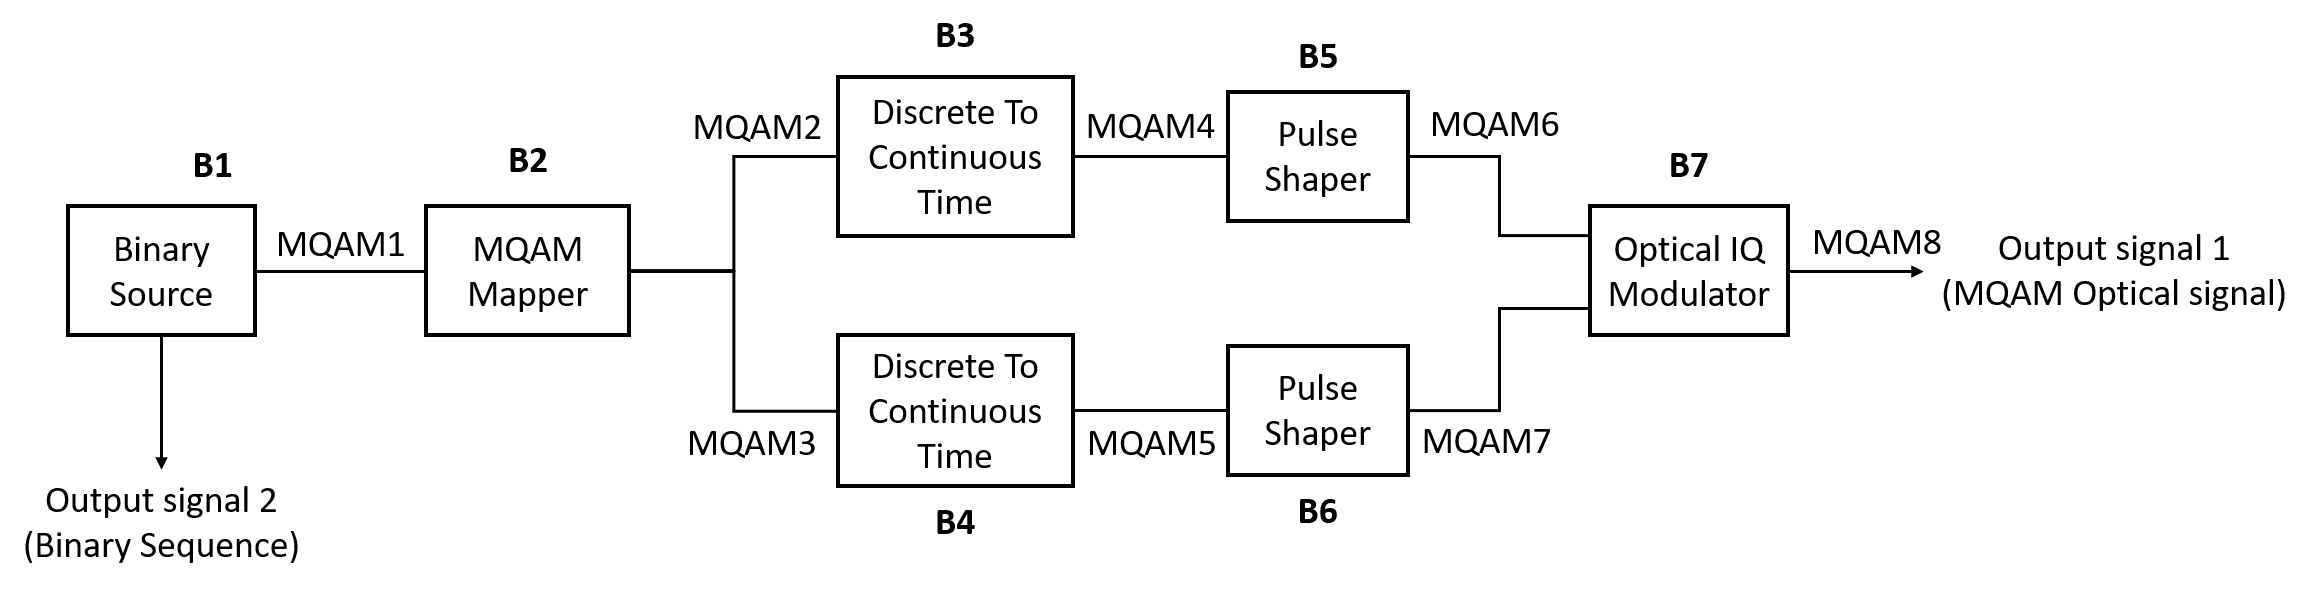
\includegraphics[width=\textwidth]{./lib/m_qam_transmitter/figures/MQAM_transmitter_block_diagram}
	\caption{Schematic representation of the block MQAM transmitter.}\label{MQAM_transmitter_block_diagram}
\end{figure}

\subsection*{Input parameters}

This block has a special set of functions that allow the user to change the basic configuration of the transmitter. The list of input parameters, functions used to change them and the values that each one can take are summarized in table \ref{table}.

\begin{table}[h]
\begin{center}
	\begin{tabular}{| m{3cm} | m{6cm} |  m{2cm} | m{4,3cm} | }
		\hline
		\textbf{Input parameters} & \textbf{Function} & Type & \textbf{Accepted values} \\ \hline
		Mode & setMode() & string & PseudoRandom \newline Random \newline DeterministicAppendZeros \newline DeterministicCyclic \\ \hline
		Number of bits generated & setNumberOfBits() & int & Any integer\\ \hline
		Pattern length & setPatternLength() & int & Real number greater than zero\\ \hline
		Number of bits & setNumberOfBits() & long & Integer number greater than zero\\ \hline
		Number of samples per symbol & setNumberOfSamplesPerSymbol() & int & Integer number of the type $2^n$ with n also integer\\ \hline
		Roll of factor & setRollOfFactor() & double & $\in$ [0,1] \\ \hline
		IQ amplitudes & setIqAmplitudes() & Vector of coordinate points in the I-Q plane & \textbf{Example} for a 4-qam mapping: \{ \{ 1.0, 1.0 \}, \{ -1.0, 1.0 \}, \{ -1.0, -1.0 \}, \{ 1.0, -1.0 \} \} \\ \hline
		Output optical power & setOutputOpticalPower() & int & Real number greater than zero\\ \hline
		Save internal signals & setSaveInternalSignals() & bool & True or False\\
		\hline
	\end{tabular}
	\caption{List of input parameters of the block MQAM transmitter} \label{table}
\end{center}
\end{table}

%\begin{itemize}
%	\item setMode(PseudoRandom);
%	\item setBitPeriod(1.0/50e9);
%	\linebreak (double)
%	\item setPatternLength(3);
%	\linebreak (int)
%	\item setNumberOfBits(10000);
%	\linebreak (long)
%	\item setNumberOfSamplesPerSymbol(32);
%	\linebreak (int)
%	\item setRollOffFactor(0.9);
%	\linebreak (double $\in$ [0,1])
%	\item setIqAmplitudes(\{ \{ 1, 1 \}, \{ -1, 1 \}, \{ -1, -1 \}, \{ 1, -1 \} \});
%	\item setOutputOpticalPower\_dBm(0);
%	\item setSaveInternalSignals(true);
%\end{itemize}

\pagebreak

\subsection*{Methods}

MQamTransmitter(vector$<$Signal *$>$ \&inputSignal, vector$<$Signal *$>$ \&outputSignal); (\textbf{constructor})
\bigbreak

void set(int opt);
\bigbreak
void setMode(BinarySourceMode m)
\bigbreak
BinarySourceMode const getMode(void)
\bigbreak
void setProbabilityOfZero(double pZero)
\bigbreak
double const getProbabilityOfZero(void)
\bigbreak
void setBitStream(string bStream)
\bigbreak
string const getBitStream(void)
\bigbreak
void setNumberOfBits(long int nOfBits)
\bigbreak
long int const getNumberOfBits(void)
\bigbreak
void setPatternLength(int pLength)
\bigbreak
int const getPatternLength(void)
\bigbreak
void setBitPeriod(double bPeriod)
\bigbreak
double const getBitPeriod(void)
\bigbreak
void setM(int mValue)
int const getM(void)
\bigbreak
void setIqAmplitudes(vector$<$t\textunderscore iqValues$>$ iqAmplitudesValues)
\bigbreak
vector$<$t\textunderscore iqValues$>$ const getIqAmplitudes(void)
\bigbreak
void setNumberOfSamplesPerSymbol(int n)
\bigbreak
int const getNumberOfSamplesPerSymbol(void)
\bigbreak
void setRollOffFactor(double rOffFactor)
\bigbreak
double const getRollOffFactor(void)
\bigbreak
void setSeeBeginningOfImpulseResponse(bool sBeginningOfImpulseResponse)
\bigbreak
double const getSeeBeginningOfImpulseResponse(void)
\bigbreak
void setOutputOpticalPower(t\textunderscore real outOpticalPower)
\bigbreak
t\textunderscore real const getOutputOpticalPower(void)
\bigbreak
void setOutputOpticalPower\_dBm(t\_real outOpticalPower\_dBm)
\bigbreak
t\_real const getOutputOpticalPower\_dBm(void)
\pagebreak

\subsection*{Output Signals}

\subparagraph*{Number:} 1 optical and 1 binary (optional)

\subparagraph*{Type:} Optical signal

\subsection*{Example}

%\begin{figure}[h]
%	\centering
%	\includegraphics[width=0.8\textwidth]{./lib/m_qam_transmitter/figures/BinarySource_output}
%	\caption{Example of the binary sequence generated by this block for a sequence 0100...}
%\end{figure}

%\begin{figure}[h]
%	\centering
%	\includegraphics[width=0.8\textwidth]{./lib/m_qam_transmitter/figures/IQmodulator0_output}
%	\caption{Example of the output optical signal generated by this block for a sequence 0100...}
%\end{figure}

\subsection*{Sugestions for future improvement}

Add to the system another block similar to this one in order to generate two optical signals with perpendicular polarizations. This would allow to combine the two optical signals and generate an optical signal with any type of polarization.

\clearpage

\section{Netxpto}

\begin{tcolorbox}	
	\begin{tabular}{p{2.75cm} p{0.2cm} p{10.5cm}} 	
		\textbf{Header File}   &:& netxpto.h\\
                               &:& netxpto\_20180118.h\\
		\textbf{Source File}   &:& netxpto.cpp \\
                               &:& netxpto\_20180118.cpp \\
	\end{tabular}
\end{tcolorbox}

This block can work in two configurations: with an external clock or without it. In the latter it accepts two input signals one being the clock and the other the signal to be demodulated. In the other configuration there's only one input signal which is the signal.

The output signal is obtained by sampling the input signal with a predetermined samplig rate provided either internally or by the clock.

\subsection*{Input Parameters}

\begin{table}[h]
	\centering
	\begin{tabular}{|c|c|p{60mm}|c|ccp{60mm}}
		\cline{1-4}
		\textbf{Parameter} & \textbf{Type} & \textbf{Values} &   \textbf{Default}& \\ \cline{1-4}
		samplesToSkip & int & any (smaller than the number of samples generated) & $0$ \\ \cline{1-4}
	\end{tabular}
	\caption{Sampler input parameters}
	\label{table:sampler_in_par}
\end{table}

%\begin{itemize}
%	\item samplesToSkip\{ 0 \}
%\end{itemize}

\subsection*{Methods}

Sampler() {}
\bigbreak
Sampler(vector$<$Signal *$>$ \&InputSig, vector$<$Signal *$>$ \&OutputSig) :Block(InputSig, OutputSig) {}
\bigbreak
void initialize(void)
\bigbreak
bool runBlock(void)
\bigbreak
void setSamplesToSkip(\texttt{t\_integer} sToSkip)

\subsection*{Functional description}

This block can work with an external clock or without it.

In the case of having an external clock it accepts two input signals. The signal to be demodulate which is complex and a clock signal that is a sequence of Dirac delta functions with a predetermined period that corresponds to the sampling period. The signal and the clock signal are scanned and when the clock has the value of 1.0 the correspondent complex value of the signal is placed in the buffer corresponding to the output signal.

There's a detail worth noting. The electrical filter has an impulse response time length of 16 (in units of symbol period). This means that when modulating a bit the spike in the signal corresponding to that bit will appear 8 units of symbol period later. For this reason there's the need to skip the earlier samples of the signal when demodulating it. That's the purpose of the \textit{samplesToSkip} parameter.

Between the binary source and the current block the signal is filtered twice which means that this effect has to be taken into account twice. Therefore the parameter \textit{samplesToSkip} is given by $2*8*samplesPerSymbol$.

\subsection*{Input Signals}

\subparagraph*{Number:} 1

\subparagraph*{Type:} Electrical real (TimeContinuousAmplitudeContinuousReal)

\subsection*{Output Signals}

\subparagraph*{Number:} 1

\subparagraph*{Type:} Electrical real (TimeDiscreteAmplitudeContinuousReal)

\subsection*{Examples}

\begin{figure}[h]
	\centering
	\includegraphics[clip, trim=0.5cm 9cm 0.5cm 9cm, width=\textwidth]{./lib/sampler/figures/MQAM_sampler_output.pdf}
	\caption{Example of the output signal of the sampler}\label{Sampler_output}
\end{figure}

\subsection{ Version 20180118}

Adds the type t\_photon\_mp\_xy, to support multi-path photon signals with polarization information.

Changes the signal data type to make private its data structure, only allowing its access through appropriate methods.


\subsection*{Sugestions for future improvement}

\clearpage

\section{Alice QKD}

\maketitle
This block is the processor for Alice does all tasks that she needs. This block accepts binary, messages, and real continuous time signals. It produces messages, binary and real discrete time signals.


\subsection*{Input Parameters}

	\begin{itemize}
		\item double RateOfPhotons\{1e3\}
	
		\item int StringPhotonsLength\{ 12 \}
	\end{itemize}

\subsection*{Methods}
    AliceQKD (vector <Signal*> \&inputSignals, vector <Signal*> \&outputSignals) : Block(inputSignals, outputSignals) \{\};

	void initialize(void);

	bool runBlock(void);

	void setRateOfPhotons(double RPhotons) \{ RateOfPhotons = RPhotons; \};
	double const getRateOfPhotons(void) \{ return RateOfPhotons; \};

	void setStringPhotonsLength(int pLength) \{ StringPhotonsLength = pLength; \};
	int const getStringPhotonsLength(void) \{ return StringPhotonsLength; \};


\subsection*{Functional description}

This block receives a sequence of binary numbers (1's or 0's) and a clock signal which will set the rate of the signals produced to generate single polarized photons. The real discrete time signal \textbf{SA\_1} is generated based on the clock signal and the real discrete time signal \textbf{SA\_2} is generated based on the random sequence of bits received through the signal \textbf{NUM\_A}. This last sequence is analysed by the polarizer in pairs of bits in which each pair has a bit for basis choice and other for direction choice.

This block also produces classical messages signals to send to Bob as well as binary messages to the mutual information block with information about the photons it sent.

\subsection*{Input Signals}
\paragraph*{Number}: 3
\paragraph*{Type}: Binary, Real Continuous Time and Messages signals.

\subsection*{Output Signals}
\paragraph*{Number}: 3
\paragraph*{Type}: Binary, Real Discrete Time and Messages signals.

\subsection*{Examples}


\subsection*{Sugestions for future improvement}




\clearpage

\section{Polarizer}

\maketitle
This block is responsible of changing the polarization of the input photon stream signal by using the information from the other real time discrete input signal. This way, this block accepts two input signals: one photon stream and other real discrete time signal. The real discrete time input signal must be a signal discrete in time in which the amplitude can be 0 or 1. The block will analyse the pairs of values by interpreting them as basis and polarization direction.


\subsection*{Input Parameters}

	\begin{itemize}
		\item m\{4\}
		\item Amplitudes \{ \{1,1\}, \{-1,1 \}, \{-1,-1 \}, \{ 1,-1\} \}
	\end{itemize}

\subsection*{Methods}

Polarizer (vector <Signal*> \&inputSignals, vector <Signal*>\&outputSignals) : Block(inputSignals, outputSignals) \{\};

void initialize(void);

bool runBlock(void);

void setM(int mValue);

void setAmplitudes(vector <t\_iqValues> AmplitudeValues);


\subsection*{Functional description}
Considering m=4, this block atributes for each pair of bits a point in space. In this case, it is be considered four possible polarization states: $0^\circ$, $45^\circ$, $90^\circ$ and $^135^\circ$.


\subsection*{Input Signals}
\subparagraph*{Number}: 2
\subparagraph*{Type}: Photon Stream and a Sequence of 0's and '1s (DiscreteTimeDiscreteAmplitude).

\subsection*{Output Signals}
\subparagraph*{Number}:1
\subparagraph*{Type}: Photon Stream

\subsection*{Examples}


\subsection*{Sugestions for future improvement} 
\clearpage

\section{Probability Estimator}

\maketitle

This blocks accepts an input binary signal and it calculates the probability of having a value "1" \space or "0" \space according to the number of samples acquired and according to the z-score value set depending on the confidence interval. It produces an output binary signal equals to the input. Nevertheless, this block has an additional output which is a txt file with information related with probability values, number of samples acquired and margin error values for each probability value.

In statistics theory, considering the results space $\Omega$ associated with a random experience and $A$ an event such that $P(A)=p\in]0,1[$. Lets $X:\Omega\longrightarrow\mathbb{R}$ such that

\begin{eqnarray}
		X(\omega) = 1&\textrm{ ,if } \omega \in A \nonumber \\
		X(\omega) = 0&\textrm{ ,if } \omega \in \bar{A} \nonumber\\
\end{eqnarray}

This way, there only are two possible results: success when the outcome is $1$ or failure when the outcome is $0$. The probability of success is $P(X=1)$ and the probability of failure is $P(X=0)$,
\begin{eqnarray}
		P(X=1) =& P(A) & = p \nonumber\\
		P(X=0) =&P(\bar{A})&=1-p  \nonumber\\
\end{eqnarray}

$X$ follows the Bernoulli law with parameter \textbf{p}, $X \sim \mathbf{B}(p)$, being the expected value of the Bernoulli random value $\textrm{E(X)}=p$ and the variance $\textrm{VAR(X)}=p(1-p)$ \cite{probabilitySheldon}.

Assuming that \textit{N} independent trials are performed, in which a success occurs with probability \textit{p} and a failure occurs with probability \textit{1-p}. If \textit{X} is the number of successes that occur in the \textit{N} trials, \textit{X} is a binomial random variable with parameters \textit{(n,p)}. Since \textit{N} is large enough, \textit{X} can be approximately normally distributed with mean $np$ and variance $np(1-p)$.
\begin{equation}\label{eq:binomialtonormal}
  \frac{X-np}{\sqrt{np(1-p)}}\backsim \emph{N}(0,1).
\end{equation}
In order to obtain a confidence interval for \textit{p}, lets assume the estimator $\hat{p}=\frac{X}{N}$ the fraction of samples equals to $1$ with regard to the total number of samples acquired. Since $\hat{p}$ is the estimator of \textit{p}, it should be approximately equal to \textit{p}. As a result, for any $\alpha \in {0,1}$ we have that:

\begin{equation}\label{eq:eq1}
   \frac{X-np}{\sqrt{n\hat{p}(1-\hat{p})}} \backsim \emph{N}(0,1) 
\end{equation}


\begin{align}\label{eq:eq2}
  \nonumber
  P \{-z_{\alpha/2} < \frac{X-np}{\sqrt{n\hat{p}(1-\hat{p})}} < z_{\alpha/2}\} &\approx& 1-\alpha \\ \nonumber
  P \{-z_{\alpha/2}\sqrt{n\hat{p}(1-\hat{p})}<np-X<z_{\alpha/2}\sqrt{n\hat{p}(1-\hat{p})}\} &\approx& 1-\alpha \\
  P\{\hat{p}-z_{\alpha/2}\sqrt{\hat{p}(1-\hat{p})/n} <p<\hat{p}+z_{\alpha/2}\sqrt{\hat{p}(1-\hat{p})/n}\} &\approx& 1-\alpha
\end{align}

This way, a confidence interval for \textit{p} is approximately $100(1-\alpha)$ percent.

\subsection*{Input Parameters}

	\begin{itemize}
		\item zscore \linebreak
		(double)
    \item fileName \linebreak
		(string)
	
	\end{itemize}

\subsection*{Methods}

ProbabilityEstimator(vector$\langle$Signal *$\rangle$ \&InputSig, vector$\langle$Signal *$\rangle$ \&OutputSig) :Block(InputSig, OutputSig)\{\};
\bigbreak	
void initialize(void);
\bigbreak	
bool runBlock(void);
\bigbreak	
void setProbabilityExpectedX(double probx)
double getProbabilityExpectedX()
\bigbreak	
void setProbabilityExpectedY(double proby)
double getProbabilityExpectedY()
\bigbreak
void setZScore(double z)
double getZScore()


\subsection*{Functional description}

This block receives an input binary signal with values "0" \space or "1" \space and it calculates the probability of having each number according with the number of samples acquired. This probability is calculated using the following formulas:
\begin{equation}\label{eq:prob1}
  \textrm{Probability}_{1}=\frac{\textrm{Number of 1's}}{\textrm{Number of Received Bits}}
\end{equation}

\begin{equation}\label{eq:prob0}
  \textrm{Probability}_{0}=\frac{\textrm{Number of 0's}}{\textrm{Number of Received Bits}}.
\end{equation}

The error margin is calculated based on the z-score set which specifies the confidence interval using the following formula:

\begin{equation}\label{eq:marginerror}
  \textrm{ME} = \textrm{z}_{\textrm{score}}\times \sqrt{\frac{\hat{p}(1-\hat{p})}{N}}
\end{equation}

being $\hat{p}$ the expected probability calculated using the formulas above and $N$ the total number of samples.

This block outputs a txt file with information regarding with the total number of received bits, the probability of 1, the probability of 0 and the respective errors.

\subsection*{Input Signals}


\subparagraph*{Number:} 1

\subparagraph*{Type:} Binary

\subsection*{Output Signals}

\subparagraph*{Number:} 2

\subparagraph*{Type:} Binary
\subparagraph*{Type:} txt file

\subsection*{Examples}


Lets calculate the margin error for N of samples in order to obtain $X$ inside a specific confidence interval, which in this case we assume a confidence interval of $99\%$.

We will use \textit{z-score } from a table about standard normal distribution, which in this case is $2.576$, since a confidence interval of $99\%$was chosen, to calculate the expected error margin,

\begin{eqnarray}
  \nonumber % Remove numbering (before each equation)
  \textrm{ME} &=&  \pm z_{\alpha/2}\frac{\sigma}{\sqrt{N}} \\
  \textrm{ME} &=& \pm z_{\alpha/2}\sqrt{\frac{\hat{p}(1-\hat{p})}{N}},
\end{eqnarray}

where, \textrm{ME} is the error margin, $z_{\alpha/2}$ is the \textit{z-score} for a specific confidence interval, $\sigma = \sqrt{\textrm{VAR(X})} = \sqrt{\hat{p}(1-\hat{p})}$ is the standard deviation and $N$ the number of samples.

This way, with a $99\%$ confidence interval, between $(\hat{p}-\textrm{ME}) \times 100$  and $(\hat{p}+\textrm{ME}) \times 100$ percent of the samples meet the standards.



\subsection*{Sugestions for future improvement}




\clearpage

\section{Bob QKD}

\maketitle
This block is the processor for Bob does all tasks that she needs. This block accepts and produces:

\begin{enumerate}
  \item 
  \item 
\end{enumerate}


\subsection*{Input Parameters}

	\begin{itemize}
		\item
		\item
		
	\end{itemize}

\subsection*{Methods}



\subsection*{Functional description}



\subsection*{Input Signals}


\subsection*{Examples}


\subsection*{Sugestions for future improvement} 
\clearpage

\section{Eve QKD}

\maketitle
This block is the processor for Eve does all tasks that she needs. This block accepts and produces:

\begin{enumerate}
    \item
    \item
\end{enumerate}


\subsection*{Input Parameters}

	\begin{itemize}
		\item
		\item
		
	\end{itemize}

\subsection*{Methods}



\subsection*{Functional description}



\subsection*{Input Signals}


\subsection*{Examples}


\subsection*{Sugestions for future improvement}

\clearpage

\section{Rotator Linear Polarizer}

\maketitle
This block accepts a Photon Stream signal and a Real discrete time signal. It produces a photon stream by rotating the polarization axis of the linearly polarized input photon stream by an angle of choice.


\subsection*{Input Parameters}
    \begin{itemize}
		\item m\{2\}
		\item axis \{ \{1,0\}, \{$\frac{\sqrt{2}}{2}$,$\frac{\sqrt{2}}{2}$ \} \}
	\end{itemize}

\subsection*{Methods}

RotatorLinearPolarizer(vector <Signal*> \&inputSignals, vector <Signal*> \&outputSignals) : Block(inputSignals, outputSignals) \{\};

void initialize(void);

bool runBlock(void);

void setM(int mValue);

void setAxis(vector <t\_iqValues> AxisValues);

\subsection*{Functional description}
This block accepts the input parameter m, which defines the number of possible rotations. In this case m=2, the block accepts the rectilinear basis, defined by the first position of the second input parameter axis, and the diagonal basis, defined by the second position of the second input parameter axis.
This block rotates the polarization axis of the linearly polarized input photon stream to the basis defined by the other input signal. If the discrete value of this signal is 0, the rotator is set to rotate the input photon stream by $0^\circ$, otherwise, if the value is 1, the rotator is set to rotate the input photon stream by an angle of $45^\circ$.


\subsection*{Input Signals}
\paragraph*{Number}: 2
\paragraph*{Type}: Photon Stream and a Sequence of 0's and '1s (DiscreteTimeDiscreteAmplitude)

\subsection*{Output Signals}
\paragraph*{Number}: 1
\paragraph*{Type}: Photon Stream

\subsection*{Examples}


\subsection*{Sugestions for future improvement} 
\clearpage

\section{Optical Switch}

\maketitle
This block has one input signal and two input signals. Furthermore, it accepts an additional input binary input signal which is used to decide which of the two outputs is activated. 


\subsection*{Input Parameters}
    No input parameters.

\subsection*{Methods}

OpticalSwitch(vector <Signal*> \&inputSignals, vector <Signal*> \&outputSignals) : Block(inputSignals, outputSignals) \{\};

void initialize(void);

bool runBlock(void);


\subsection*{Functional description}
This block receives an input photon stream signal and it decides which path the signal must follow. In order to make this decision it receives a binary signal (0's and 1's) and it switch the output path according with this signal.

\subsection*{Input Signals}
\paragraph*{Number}: 1
\paragraph*{Type}: Photon Stream

\subsection*{Output Signals}
\paragraph*{Number}: 2
\paragraph*{Type}: Photon Stream

\subsection*{Examples}


\subsection*{Sugestions for future improvement} 
\clearpage

\section{Optical Hybrid}

\begin{tcolorbox}	
	\begin{tabular}{p{2.75cm} p{0.2cm} p{10.5cm}} 	
		\textbf{Header File}   &:& optical\_hybrid.h \\
		\textbf{Source File}   &:& optical\_hybrid.cpp \\
	\end{tabular}
\end{tcolorbox}

This block simulates an optical hybrid. It accepts two input signals corresponding to the signal and to the local oscillator. It generates four output complex signals separated by $90^\circ$ in the complex plane. Figure ~\ref{opticalhybrid} shows a schematic representation of this block.

\begin{figure}[h]
	\centering\includegraphics[width=0.6\textwidth]{./lib/optical_hybrid/figures/optical_hybrid_block_diagram.png}
	\caption{Schematic representation of an optical hybrid.}\label{opticalhybrid}
\end{figure}

\subsection*{Input Parameters}

\begin{table}[h]
	\centering
	\begin{tabular}{|c|c|c|c|ccp{60mm}}
		\cline{1-4}
		\textbf{Parameter} & \textbf{Type} & \textbf{Values} &   \textbf{Default}& \\ \cline{1-4}
		outputOpticalPower & double & any & $1e-3$ \\ \cline{1-4}
		outputOpticalWavelength & double & any & $1550e-9$ \\ \cline{1-4}
		outputOpticalFrequency & double & any & SPEED\_OF\_LIGHT / outputOpticalWavelength \\ \cline{1-4}
		powerFactor & double & $\leq 1$ & $0.5$ \\ \cline{1-4} 
	\end{tabular}
	\caption{Optical hybrid input parameters}
	\label{table:optical_hybrid_in_par}
\end{table}

%\begin{itemize}
%	\item outputOpticalPower\{ 1e-3 \} 
%	\item outputOpticalWavelength\{ 1550e-9 \}
%	\item outputOpticalFrequency\{ SPEED\_OF\_LIGHT / wavelength \}
%	\item powerFactor\{0.5\}
%\end{itemize}

\subsection*{Methods}
 
OpticalHybrid() {}
\bigbreak
OpticalHybrid(vector$<$Signal *$>$ \&InputSig, vector$<$Signal *$>$ \&OutputSig) :Block(InputSig, OutputSig) {}
\bigbreak
void initialize(void)
\bigbreak
bool runBlock(void)
\bigbreak
void setOutputOpticalPower(double outOpticalPower)
\bigbreak
void setOutputOpticalPower\_dBm(double outOpticalPower\_dBm)
\bigbreak
void setOutputOpticalWavelength(double outOpticalWavelength)
\bigbreak
void setOutputOpticalFrequency(double outOpticalFrequency) 
\bigbreak
void setPowerFactor(double pFactor)

\subsection*{Functional description}

This block accepts two  input signals corresponding to the signal to be demodulated ($S$) and to the local oscillator ($L$). It generates four output optical signals given by $\textit{powerFactor}\times(S+L)$, $\textit{powerFactor}\times(S-L)$,$\textit{powerFactor}\times(S+iL)$, $\textit{powerFactor}\times(S-iL)$. The input parameter \textit{powerFactor} assures the conservation of optical power.

\subsection*{Input Signals}

\subparagraph*{Number:} 2

\subparagraph*{Type:} Optical (OpticalSignal)

\subsection*{Output Signals}

\subparagraph*{Number:} 4

\subparagraph*{Type:} Optical (OpticalSignal)

\subsection*{Examples} 

%\begin{figure}[h]
%	\centering
%	\includegraphics[width=\textwidth]{./lib/optical_hybrid/MQAM_optical_hybrid_output.pdf}
%	\caption{Example of one of the output signals of this block for a binary sequence 01}\label{OpticalHybrid_output}
%\end{figure}

\subsection*{Sugestions for future improvement}

\documentclass[../../sdf/tex/BPSK_system.tex]{subfiles}
\graphicspath{{../../images/}}
%opening
\onlyinsubfile{\title{Photodiode}}
\date{}

\begin{document}

\onlyinsubfile{\maketitle}

\subsection*{Input Parameters}

\begin{multicols}{2}
	\begin{itemize}
		\item setResponsivity
		\item useNoise
	\end{itemize}
\end{multicols}

\subsection*{Functional Description}

This block accepts two complex signals and outputs one real signal built from an evaluation of the power of the input signals and their subsequent subtraction. The responsivity is defined by the value of \textit{Responsivity}. This block also adds random gaussian distributed shot noise with an amplitude defined by the power of the inputs. The shot noise is activated by the boolean variable set by the \textit{useNoise} parameter.


\subsection*{Low pass representation conversion}

The transmission of signal uses a carrier frequency, which is modulated in amplitude and in phase. Given the high frequency of this carrier signal ($\approx 10^(14) Hz$), the simulation of it would be very hard, so, the Low Pass Representation is used instead. In practice, after modulation, the signal shows a negative and a positive band in the frequency space. To obtain the Low Pass Representation, we start by filtering the signal, outputting only the positive band. This step reduces the energy of the signal to one half of the original. After that, a frequency downshift is made, using the negative of the frequency of the carrier signal.\\
Because a local oscillator will output the Low Pass Representation of a beam, the output power will be $\tilde{P}=\frac{1}{2}P$, in which $P$ is the power of the laser. This will also scale the amplitude of the output signal by $\frac{1}{\sqrt{2}}$.\\
Therefore, given a input signal in the photodiode with amplitude $\tilde{\Psi}$, to recover $P$, we must use:
\begin{equation}
P = 2 |\tilde{\Psi}|^2
\end{equation}


\subsection*{Noise implementation}

{\bf Quantum Noise}\\
The photodiode's out current is modelled as the conversion of the input optical power, which follows the photon number statistics. Using $n$ as the number of input photons, and assuming their source as laser light, we know that this stochastic variable follows:
%
\begin{equation}
n \sim \textrm{Poisson}(\braket{n})
\end{equation}
%
In the simulation, the input of a photodiode corresponds to a mean complex amplitude $\bar{\Psi}$. This amplitude corresponds to the power $\bar{P} = |\bar{\Psi}|^2 = \braket{n}P_\lambda$ in which $P_\lambda$ is the power of a single photon. We want the resulting power after adding noise, $P = n P_\lambda$. To model $n$, we will use a gaussian aproximation of $\sqrt{n}$, for $n \gg 0$, which will give us a continuous distribution:
%
\begin{equation}
\sqrt{n} \sim \textrm{Gaussian}(\sqrt{\braket{n}}, 1/2)
\end{equation}
%
Therefore:
%
\begin{equation}
n \approx \left( \sqrt{\braket{n}} + \frac{1}{2}G \right)^2 = \braket{n} + \sqrt{\braket{n}} G + \frac{1}{4} G^2
\end{equation}
%
in which $G$ is a random variable with a gaussian distribution with mean $0$ and variance $1$.\\
Therefore, the output power of each becomes:
%
\begin{equation}
P = n P_\lambda = \bar{P} + \sqrt{P_\lambda \bar{P}} G + \frac{1}{4} P_\lambda G^2
\end{equation}
%
\\
\\
{\bf Thermal Noise}\\
In the experimental setting, it is assumed that this noise is created by the detection system. To simulate this noise, the photodiode will add it to the output current as a simple gaussian distribution with mean $0$ and variance according to experimental settings.\\

\subsection*{Input Signals}

\textbf{Number}: 2

\textbf{Type}: Complex signal (ContinuousTimeContinuousAmplitude)

\subsection*{Output Signals}

\textbf{Number}: 1

\textbf{Type}: Real signal (ContinuousTimeContinuousAmplitude)

\end{document}

\clearpage

\section{Photoelectron Generator}

\begin{refsection}

\begin{tcolorbox}	
\begin{tabular}{p{2.75cm} p{0.2cm} p{10.5cm}} 	
\textbf{Header File}   &:& photoelectron\_generator\_*.h \\
\textbf{Source File}   &:& photoelectron\_generator\_*.cpp \\
\textbf{Version}       &:& 20180302 (Diamantino Silva)
\end{tabular}
\end{tcolorbox}

\vspace{1em}

This block simulates the generation of photoelectrons by a photodiode, performing the conversion of an incident electric field into an output current proportional to the field's instantaneous power.
It is also capable of simulating shot noise.
%
\begin{figure}[h]
	\centering
	\includegraphics{./lib/photoelectron_generator/figures/photoelectron_generator_scheme.pdf}
	\caption{Schematic representation of the photoelectron generator code block}
\end{figure}

\subsection*{Theoretical description}

The operation of a real photodiode is based on the photoelectric effect, which consists on the removal of one electron from the target material by a single photon, with a probability $\eta$.
Given an input beam with an optical power $P(t)$ in which the photons are around the wavelength $\lambda$, the flux of photons $\phi(t)$ is calculated as
\cite{saleh1991}
%
\begin{equation}
	\phi(t) = \frac{P(t) \lambda}{hc}
\end{equation}
therefore, the mean number of photons in a given interval $\left[ t, t+T \right[$ is
\begin{equation}
	\bar{n}(t) = \int_{t}^{t+T} \phi(\tau) \; \textrm{d}\tau
\end{equation}
%
But the actual number of photons in a given time interval, $n(t)$, is random. If we assume that the electric field is generated by an ideal laser with constant power, then $n(t)$ will follow a Poisson distribution
%
\begin{equation}
	p\left( n \right) = \frac{ \bar{n}^n \exp(-\bar{n})}{n!}
\end{equation}
%
where $n=n(t)$ and $\bar{n} = \bar{n}(t)$.
\\
For each incident photon, there is a probability $\eta$ of generating a phototelectron.
Therefore, we can model the generation of photoelectrons during this time interval, as a binomial process where the number of events is equal to the number of incident photons, $n(t)$, and the rate of success is $\eta$.
If we combine the two random processes, binomial photoelectron generation after poissonian photon flux, the number of output photoelectrons in this time interval, $m(t)$, will follow
\cite{saleh1991}
%
\begin{equation}
	m \sim \textrm{Poisson}\left(\eta \bar{n} \right)
	\label{eq:electron_number_distribution}
\end{equation}
%
with $\bar{m} = \eta \bar{n}$ where $m = m(t)$.
%
%
%
%
\subsection*{Functional description}
%
The input of this block is the electric field amplitude, $A(t)$, with sampling period $T$.
The first step consists on the calculation the instantaneous power.
Given that the input amplitude is a baseband representation of the original signal, then $P(t) = 4 |A(t)|^2$.
From this result, the average number of photons $\bar{n}(t) = T P(t) \lambda / h c$.\\
If the shot-noise is negleted, then the output number of photoelectrons, $n_e(t)$ in the interval, will be equal to
%
\begin{equation}
	m(t) = \eta \overline{n(t)}
\end{equation}
%
If the shot-noise is considered, then the output fluctuations will be simulated by generating a value from a Poissonian random number generator with mean $\eta \overline{n(t)}$
\begin{equation}
	m(t) \sim \textrm{Poisson}\left(\eta \overline{n(t)} \right)
\end{equation}

\subsection*{Input Parameters}

\begin{table}[H]
	\centering
	\label{my-label}
	\begin{tabular}{|c|c|c|}
		\hline
		\textbf{Parameter}	& \textbf{Default Value}	& \textbf{Description} \\
		\hline
		efficiency			& 1.0						& Photodiode's quantum efficiency. \\
		\hline
		shotNoise			& false 					& Shot-noise off/on. \\
		\hline
	\end{tabular}
\end{table}




\subsection*{Methods}

PhotoelectronGenerator()
\bigbreak
PhotoelectronGenerator(vector$<$Signal *$>$ \&InputSig, vector$<$Signal *$>$ \&OutputSig) :Block(InputSig, OutputSig) {}
\bigbreak
void initialize(void)
\bigbreak
bool runBlock(void)
\bigbreak
void setEfficiency(\texttt{t\_real} efficiency)
\bigbreak
void getEfficiency()
\bigbreak
void setShotNoise(\texttt{bool} shotNoise)
\bigbreak
void getShotNoise()
%
%
%
%
\pagebreak

\subsection*{Input Signals}

\subparagraph*{Number:} 1

\subparagraph*{Type:} Optical (OpticalSignal)

\subsection*{Output Signals}

\subparagraph*{Number:} 1

\subparagraph*{Type:} Electrical (TimeDiscreteAmplitudeContinuousReal or TimeContinuousAmplitudeContinuousReal)

\subsection*{Examples}

\begin{figure}[h]
	\centering
	\includegraphics{./lib/photoelectron_generator/figures/scheme_simulation_constant.pdf}
	\caption{Constant power simulation setup}
\end{figure}

To test the output of this block, we recreated the results of figure $11.2-3$ in \cite{saleh1991}.
We started by simulating the constant optical power case, in which the local oscillator power was fixed to a constant value.
Two power levels were tested, $P = 1 \mu W$ and $P = 1 nW$, using a sample period of $20$ picoseconds and photoelectron generator efficiency of $1.0$.
The simulation code is in folder \texttt{lib \textbackslash photoelectron\_generator \textbackslash photoelectron\_generator\_test\_constant}.
The following plots show the number of output electrons per sample when the shot noise is ignored or considered

\begin{figure}[H]
	\centering
	\begin{subfigure}{0.45\textwidth}
		\includegraphics[width=\textwidth]{./lib/photoelectron_generator/figures/plot-constant-1uW}
		\caption{$P=1 \mu W$}
	\end{subfigure}
	\hspace{10mm}
	\begin{subfigure}{0.45\textwidth}
		\includegraphics[width=\textwidth]{./lib/photoelectron_generator/figures/plot-constant-1nW}
		\caption{$P=1 nW$}
	\end{subfigure}
	\caption{Upper plots: input optical squared amplitude on the photoelectron generator; Middle plots: number of output photoelectrons per sample neglecting quantum noise; Bottom plots: number of output photoelectrons per sample considering quantum noise.}
	\label{plot:quantum_noise_sim_constant}
\end{figure}
%
Figure \ref{plot:quantum_noise_sim_constant} shows clearly that turning the quantum noise on or off will produce a signal with or without variance, as predicted.
If we compare this result with plot $(a)$ in \cite{saleh1991}, in particular $P=1nW$, we see that they are in conformance, with a slight difference, where a sample has more than one photoelectron.
In constrast with the reference result, where only single events are represented, the $P=1 \mu W$ case shows that all samples account many photoelectrons.
Given it's input power, multiple photoelectron generation events will occur during the sample time window.
Therefore, to recreate the reference result, we just need to reduce the sample period until the probability of generating more than $1$ photoelectron per sample goes to $0$.
\\
%
\begin{figure}[H]
	\centering
	\includegraphics{./lib/photoelectron_generator/figures/scheme_simulation_variable.pdf}
	\caption{Variable power simulation setup}
\end{figure}
%
To recreate plot $(b)$ in \cite{saleh1991}, a more complex setup was used, where a series of states are generated and shaped by a MQAM, creating a input electric field with time-varying power.\\
The simulation code is in folder \texttt{lib \textbackslash photoelectron\_generator \textbackslash photoelectron\_generator\_test\_variable}.
%
\begin{figure}[H]
	\centering
	\includegraphics[width=0.45\textwidth]{./lib/photoelectron_generator/figures/plot-variable}
	\caption{Upper plots: input optical squared amplitude on the photoelectron generator; Middle plots: number of output photoelectrons per sample neglecting quantum noise; Bottom plots: number of output photoelectrons per sample considering quantum noise.}
	\label{plot:quantum_noise_sim_variable}
\end{figure}
%
Figure \ref{plot:quantum_noise_sim_variable} shows that the output without shot-noise is following the input power perfectly, apart from a constant factor. In the case with shot-noise, we see a that there are only output samples in high power input samples.\\
These results are not following strictly plot $(b)$ in \cite{saleh1991}, because has already discussed previously, in the high power input samples, we have a great probability of generating many photoelectrons.
%
\subsection*{Sugestions for future improvement}


% bibliographic references for the section ----------------------------
\clearpage
\printbibliography[heading=subbibliography]
\end{refsection}
\addcontentsline{toc}{subsection}{Bibliography}
\cleardoublepage
% ---------------------------------------------------------------------



%\bibliography{./lib/photoelectron_generator/photoelectron_generator}

\clearpage

\section{Pulse Shaper}

\begin{tcolorbox}	
	\begin{tabular}{p{2.75cm} p{0.2cm} p{10.5cm}} 	
		\textbf{Header File}   &:& pulse\_shaper.h \\
		\textbf{Source File}   &:& pulse\_shaper.cpp \\
	\end{tabular}
\end{tcolorbox}

This block applies an electrical filter to the signal. It accepts one input signal that is a sequence of Dirac delta functions and it produces one output signal continuous in time and in amplitude.

\subsection*{Input Parameters}

\begin{table}[h]
	\centering
	\begin{tabular}{|c|c|p{60mm}|c|ccp{60mm}}
		\cline{1-4}
		\textbf{Parameter} & \textbf{Type} & \textbf{Values} &   \textbf{Default}& \\ \cline{1-4}
		filterType & string & RaisedCosine, Gaussian & RaisedCosine \\ \cline{1-4}
		impulseResponseTimeLength & int & any & $16$ \\ \cline{1-4}
		rollOfFactor & real & $\in \left[0,1\right]$ & $0.9$ \\ \cline{1-4} 
	\end{tabular}
	\caption{Pulse shaper input parameters}
	\label{table:pulse_shaper_in_par}
\end{table}

%\begin{itemize}
%	\item filterType\{RaisedCosine\} \linebreak
%	\item impulseResponseTimeLength\{16\}\linebreak (int) 
%	\linebreak (This parameter is given in units of symbol period)
%	\item rollOfFactor\{0.9\} \linebreak
%	(real $\in$ [0,1])
%\end{itemize}

\subsection*{Methods}

PulseShaper(vector$<$Signal *$>$ \&InputSig, vector$<$Signal *$>$ OutputSig) :FIR$\_$Filter(InputSig, OutputSig)\{\};
\bigbreak	
void initialize(void);
\bigbreak	
void setImpulseResponseTimeLength(int impResponseTimeLength)
\bigbreak
int const getImpulseResponseTimeLength(void)
\bigbreak	
void setFilterType(PulseShaperFilter fType)
\bigbreak
PulseShaperFilter const getFilterType(void)
\bigbreak	
void setRollOffFactor(double rOffFactor)
\bigbreak
double const getRollOffFactor()

\subsection*{Functional Description}

The type of filter applied to the signal can be selected trough the input parameter \textit{filterType}. Currently the only available filter is a raised cosine.

The filter's transfer function is defined by the vector \textit{impulseResponse}. The parameter \textit{rollOfFactor} is a characteristic of the filter and is used to define its transfer function.

\subsection*{Input Signals}

\subparagraph*{Number}: 1

\subparagraph*{Type}: Sequence of Dirac Delta functions (ContinuousTimeDiscreteAmplitude)

\subsection*{Output Signals}

\subparagraph*{Number}: 1

\subparagraph*{Type}: Sequence of impulses modulated by the filter (ContinuousTimeContinuousAmplitude)

\subsection*{Example}

\begin{figure}[h]
	\centering
	\includegraphics[clip, trim=0.5cm 9cm 0.5cm 9cm, width=\textwidth]{./lib/pulse_shaper/figures/MQAM_pulse_shaper_output.pdf}
	\label{MQAM6_DeterministicAppendZeros}\caption{Example of a signal generated by this block for the initial binary signal 0100...}
\end{figure}

\subsection*{Sugestions for future improvement}

Include other types of filters.

\clearpage

\section{Quantizer}

\begin{tcolorbox}	
	\begin{tabular}{p{2.75cm} p{0.2cm} p{10.5cm}} 	
		\textbf{Header File}   &:& quantizer$\_*$.h \\
		\textbf{Source File}   &:& quantizer$\_*$.cpp \\
        \textbf{Version}       &:& 20180423 (Celestino Martins) \\
	\end{tabular}
\end{tcolorbox}

This block simulates a quantizer, where the signal is quantized into discrete levels. Given a quantization bit precision, $resolution$, the outputs signal will be comprise $2^{nBits}-1$ levels.

\subsection*{Input Parameters}

\begin{table}[h]
	\centering
	\begin{tabular}{|c|c|c|c|c|cccc}
		\cline{1-4}
		\textbf{Parameter} & \textbf{Unity} & \textbf{Type} & \textbf{Values} &   \textbf{Default}& \\ \cline{1-5}
		resolution & bits  & double & any & $inf$ \\ \cline{1-5}	
        maxValue   & volts & double & any & $1.5$ \\ \cline{1-5}	
        minValue   & volts & double & any    & $-1.5$ \\ \cline{1-5}	
	\end{tabular}
	\caption{Quantizer input parameters}
	\label{table:quantizer_in_par}
\end{table}


\subsection*{Methods}

Quantizer() {};
\bigbreak
Quantizer(vector$<$Signal *$>$ \&InputSig, vector$<$Signal *$>$ \&OutputSig) :Block(InputSig, OutputSig)\{\};
\bigbreak
void initialize(void);
\bigbreak
bool runBlock(void);
\bigbreak
void setSamplingPeriod(double sPeriod) { samplingPeriod = sPeriod; }
\bigbreak
void setSymbolPeriod(double sPeriod) { symbolPeriod = sPeriod; }
\bigbreak
void setResolution(double nbits) { resolution = nbits; }
\bigbreak
double getResolution() { return resolution; }
\bigbreak
void setMinValue(double maxvalue) { maxValue = maxvalue; }
\bigbreak
double getMinValue() { return maxValue; }
\bigbreak
void setMaxValue(double maxvalue) { maxValue = maxvalue; }
\bigbreak
double getMaxValue() { return maxValue; }

\subsection*{Functional description}

This block can performs the signal quantization according to the defined input parameter \textit{resolution}.

Firstly, the parameter \textit{resolution} is checked and if it is equal to the infinity, the output signal correspond to the input signal. Otherwise, the quantization process is applied. The input signal is quantized into $2^{resolution-1}$ discrete levels using the standard \textit{round} function.

\pagebreak
\subsection*{Input Signals}

\subparagraph*{Number:} 1

\subsection*{Output Signals}

\subparagraph*{Number:} 1

\subparagraph*{Type:} Electrical complex signal

\subsection*{Examples}

\subsection*{Sugestions for future improvement}



\clearpage

\section{Resample}

\begin{tcolorbox}	
	\begin{tabular}{p{2.75cm} p{0.2cm} p{10.5cm}} 	
		\textbf{Header File}   &:& resample$\_*$.h \\
		\textbf{Source File}   &:& resample$\_*$.cpp \\
        \textbf{Version}       &:& 20180423 (Celestino Martins) \\
	\end{tabular}
\end{tcolorbox}

This block simulates the resampling of a signal. It receives one input signal and outputs a signal with the sampling rate defined by sampling rate, which is externally configured.

\subsection*{Input Parameters}

\begin{table}[h]
	\centering
	\begin{tabular}{|c|c|c|c|cccc}
		\cline{1-4}
		\textbf{Parameter} & \textbf{Type} & \textbf{Values} &   \textbf{Default}& \\ \cline{1-4}
		rFactor           & double & any & $inf$ \\ \cline{1-4}
		samplingPeriod    & double & any & $0.0$ \\ \cline{1-4}	
        symbolPeriod      & double & any & $1.5$ \\ \cline{1-4}	
	\end{tabular}
	\caption{Resample input parameters}
	\label{table:resample_in_par}
\end{table}


\subsection*{Methods}

Resample() {};
Resample(vector$<$Signal *$>$ \&InputSig, vector$<$Signal *$>$ \&OutputSig) :Block(InputSig, OutputSig)\{\};

void initialize(void);
bool runBlock(void);

void setSamplingPeriod(double sPeriod) { samplingPeriod = sPeriod; }
void setSymbolPeriod(double sPeriod) { symbolPeriod = sPeriod; }

void setOutRateFactor(double OUTsRate) { rFactor = OUTsRate; }
double getOutRateFactor() { return rFactor; }

\subsection*{Functional description}

This block can performs the signal resample according to the defined input parameter \textit{rFactor}. It resamples the input signal at rFactor times the original sample rate.

Firstly, the parameter \textit{nBits} is checked and if it is greater than 1 it is performed a linear interpolation, increasing the input signal original sample rate to rFactor times.


\pagebreak
\subsection*{Input Signals}

\subparagraph*{Number:} 1

\subsection*{Output Signals}

\subparagraph*{Number:} 1

\subparagraph*{Type:} Electrical complex signal

\subsection*{Examples}

\subsection*{Sugestions for future improvement}



\clearpage

\section{Sampler}

\begin{tcolorbox}	
	\begin{tabular}{p{2.75cm} p{0.2cm} p{10.5cm}} 	
		\textbf{Header File}   &:& sampler.h \\
		\textbf{Source File}   &:& sampler\_20171119.cpp \\
	\end{tabular}
\end{tcolorbox}

This block can work in two configurations: with an external clock or without it. In the latter it accepts two input signals one being the clock and the other the signal to be demodulated. In the other configuration there's only one input signal which is the signal.

The output signal is obtained by sampling the input signal with a predetermined sampling rate provided either internally or by the clock.

\subsection*{Input Parameters}

\begin{table}[h]
	\centering
	\begin{tabular}{|c|c|p{60mm}|c|ccp{60mm}}
		\cline{1-4}
		\textbf{Parameter} & \textbf{Type} & \textbf{Values} &   \textbf{Default}& \\ \cline{1-4}
		samplesToSkip & int & any (smaller than the number of samples generated) & $0$ \\ \cline{1-4}
	\end{tabular}
	\caption{Sampler input parameters}
	\label{table:sampler_in_par}
\end{table}

%\begin{itemize}
%	\item samplesToSkip\{ 0 \}
%\end{itemize}

\subsection*{Methods}

Sampler() {}
\bigbreak
Sampler(vector$<$Signal *$>$ \&InputSig, vector$<$Signal *$>$ \&OutputSig) :Block(InputSig, OutputSig) {}
\bigbreak
void initialize(void)
\bigbreak
bool runBlock(void)
\bigbreak
void setSamplesToSkip(\texttt{t\_integer} sToSkip)

\subsection*{Functional description}

This block can work with an external clock or without it.

In the case of having an external clock it accepts two input signals. The signal to be demodulate which is complex and a clock signal that is a sequence of Dirac delta functions with a predetermined period that corresponds to the sampling period. The signal and the clock signal are scanned and when the clock has the value of 1.0 the correspondent complex value of the signal is placed in the buffer corresponding to the output signal.

There's a detail worth noting. The electrical filter has an impulse response time length of 16 (in units of symbol period). This means that when modulating a bit the spike in the signal corresponding to that bit will appear 8 units of symbol period later. For this reason there's the need to skip the earlier samples of the signal when demodulating it. That's the purpose of the \textit{samplesToSkip} parameter.

Between the binary source and the current block the signal is filtered twice which means that this effect has to be taken into account twice. Therefore the parameter \textit{samplesToSkip} is given by $2*8*samplesPerSymbol$.

\subsection*{Input Signals}

\subparagraph*{Number:} 1

\subparagraph*{Type:} Electrical real (TimeContinuousAmplitudeContinuousReal)

\subsection*{Output Signals}

\subparagraph*{Number:} 1

\subparagraph*{Type:} Electrical real (TimeDiscreteAmplitudeContinuousReal)

\subsection*{Examples}

\begin{figure}[h]
	\centering
	\includegraphics[clip, trim=0.5cm 9cm 0.5cm 9cm, width=\textwidth]{./lib/sampler/figures/MQAM_sampler_output.pdf}
	\caption{Example of the output signal of the sampler}\label{Sampler_output}
\end{figure}

\subsection*{Sugestions for future improvement}

\clearpage

\begin{refsection}

\section{SNR of the Photoelectron Generator}

\begin{tcolorbox}	
\begin{tabular}{p{2.75cm} p{0.2cm} p{10.5cm}} 	
\textbf{Header File}   &:& srn\_photoelectron\_generator\_*.h \\
\textbf{Source File}   &:& snr\_photoelectron\_generator\_*.cpp \\
\textbf{Version}       &:& 20180309 (Diamantino Silva)
\end{tabular}
\end{tcolorbox}

\vspace{1em}
%
This block estimates the signal to noise ratio (SNR) of a input stream of photoelectrons, for a given time window.
%
\begin{figure}[h]
	\centering
	\includegraphics{./lib/snr_photoelectron_generator/figures/snr_photoelectron_generator_scheme.pdf}
	\caption{Schematic representation of the SNR of the Photoelectron Generator code block}
\end{figure}

\subsection*{Theoretical description}
%
The input of this block is a stream of samples, $y_j$, each one of them corresponding to a number of photoelectrons generated in a time interval $\Delta t$. These photoelectrons are usually the output of a photodiode (photoelectron generator).
To calculate the SNR of this stream, we will use the definition used in
\cite{saleh1991}
%
\begin{equation}
	\textrm{SNR} = \frac{\bar{n}^2}{\sigma_n^2}
\end{equation}
%
in which $\bar{n}$ is the mean value and $\sigma_n^2$ is the variance of the photon number in a given time interval $T$.
\\
To apply this definition to our input stream, we start by separate it's samples in contiguous time windows with duration $T$. Each time window $k$ is defined as the time interval $\left[ k T, (k+1) T \right[$. To estimate the SNR for each time window, we will use the following estimators for the mean, $\mu_k$, and variance, $s_k^2$
\cite{smith1997}
%
\begin{equation}
	\mu_k = \braket{y}_k
	\qquad \qquad
	s_k^2 = \frac{N}{N-1} \left( \braket{y^2}_k - \braket{y}_k^2 \right)
\end{equation}
%
were $\braket{y^n}_k$ is the $n$ moment of the $k$ window given by
%
\begin{equation}
	\braket{y^n}_k = \frac{1}{N_k} \sum_{j = j_\textrm{min}(k)}^{j_\textrm{max}(k)} y_j^n
\end{equation}
in which
\begin{align}
	j_{min}(k) &= \lceil{t_k/\Delta t \rceil}\\
	\label{eq:sample_limit_min}
	j_{max}(k) &= \lceil{t_{k+1}/\Delta t \rceil} - 1\\
	\label{eq:sample_limit_max}
	N_k &= j_{max}(k) - j_{min}(k) + 1\\
	\label{eq:n_window_samples}
	t_k &= k T
\end{align}
where $\lceil x \rceil$ is the ceiling function.\\
%
In our implementation, we define two variables, $S_1(k)$ and $S_2(k)$, corresponding to the sum of the samples and the sum of the squares of the sample in the time interval $k$.
These two sums are related to the moments as
\begin{align}
	S_1(k) &= N_k \braket{y}_k\\
	S_2(k) &= N_k \braket{y^2}_k
\end{align}
Using these two variables, we can rewrite $\mu_k$ and $s^2_k$ as
\begin{equation}
	\mu_k = \frac{S_1(k)}{N_k}
	\qquad \qquad
	s_k^2 = \frac{1}{N_k-1} \left( S_2(k) - \frac{1}{N_k}(S_1(k))^2 \right)
\end{equation}
The signal to noise ratio of the time interval $k$, $\textrm{SNR}_k$, can be expressed as
\begin{equation}
	\textrm{SNR}_k = \frac{\mu_k^2}{\sigma_k^2} =  \frac{N_k - 1}{N_k}\frac{(S_1(k))^2}{N_k S_2(k) - (S_1(k))^2}
	\label{eq:snr_estimation}
\end{equation}
%
One particularly important case is the phototelectron stream resulting from the conversion of a laser photon stream by a photodiode (photoelectron generator). The resulting SNR will be
\cite{saleh1991}
%
\begin{equation}
	\textrm{SNR} = \eta \bar{n}
	\label{eq:ideal_poisson_snr}
\end{equation}
in which $\eta$ is the photodiode quantum efficiency.
%
\subsection*{Functional description}
%
This block is designed to operate in time windows, dividing the input stream in contiguous sets of samples with a duration $\texttt{tWindow} = T$.
For each time window, the general process consists in accumulating the input sample values and the square of the input sample values, and calculating the SNR of the time window based on these two variables.\\
To process this accumulation, the block uses two state variables, \texttt{aux\_sum1} and \texttt{aux\_sum2}, which hold the accumulation of the sample values and accumulation of the square of sample values, respectively.\\
The block starts by calculating the number of samples it has to process for the current time window, using equations \ref{eq:sample_limit_min}, \ref{eq:sample_limit_max} and \ref{eq:n_window_samples}.
If the duration of \texttt{tWindow} is $0$, then we assume that this time window has infinite time (infinite samples).
The values of \texttt{aux\_sum1} and \texttt{aux\_sum2} are set to $0$, and the processing of the samples of current window begins.\\
After processing all the samples of the time window, we obtain $S1(k)$ and $S2(k)$ from the state variables as $S1(k) = \texttt{aux\_sum1}$ and $S_2(k) = \texttt{aux\_sum2}$, and proceed to the calculation of the $\textrm{SNR}_k$, using equation \ref{eq:snr_estimation}.\\
If the simulation ends before reaching the end of the current time window, we calculate the $\textrm{SNR}_k$, using the current values of \texttt{aux\_sum1}, \texttt{aux\_sum2} for $S_1(k)$ and $S_2(k)$, and the number of samples already processed, $\texttt{currentWindowSample}$, for $N_k$.
%
%
%
%
\subsection*{Input Parameters}

\begin{table}[H]
	\centering
	\begin{tabular}{|c|c|c|}
		\hline
		\textbf{Parameter}	& \textbf{Default Value}	& \textbf{Description} \\
		\hline
		windowTime			& 0							& SNR time window. \\
		\hline
		%confidenceInterval	& 0.9						& Output SNR confidence interval. \\
		%\hline
	\end{tabular}
\end{table}




\subsection*{Methods}

SnrPhotoelectronGenerator() {}
\bigbreak
SnrPhotoelectronGenerator(vector$<$Signal *$>$ \&InputSig, vector$<$Signal *$>$ \&OutputSig) :Block(InputSig, OutputSig) {}
\bigbreak
void initialize(void)
\bigbreak
bool runBlock(void)
\bigbreak
void setTimeWindow(\texttt{t\_real} timeWindow)
%\bigbreak
%void setConfidenceInterval(\texttt{t\_real} confidenceInterval)
%
%
%
%
\pagebreak

\subsection*{Input Signals}

\subparagraph*{Number:} 1

\subparagraph*{Type:} Electrical (TimeDiscreteAmplitudeContinuousReal)

\subsection*{Output Signals}

\subparagraph*{Number:} 1

\subparagraph*{Type:} Electrical (TimeDiscreteAmplitudeContinuousReal)

\subsection*{Examples}

\begin{figure}[h]
	\centering
	\includegraphics[width=\textwidth]{./lib/snr_photoelectron_generator/figures/scheme-simulation.pdf}
	\caption{Simulation setup}
\end{figure}

To confirm the block's correct output, we have designed a simulation setup which calculates the SNR of a stream of photoelectrons generated by the detection of a laser photon stream by a photodiode.\\
The simulation has three main parameters, the power of the local oscillator, $P_{LO}$, the duration of the time window, $T$, and the photodiode's quantum efficiency, $\eta$. For each combination of these three parameters, the simulation generates $1000$ SNR samples, during which all parameters stay constant.
The final result is the average of these SNR samples.\\
The simulations were performed with a sample time $\Delta t = 10^{-10} s$.
%
\begin{figure}[H]
	\centering
	\begin{subfigure}{0.45\textwidth}
		\includegraphics[width=\textwidth]{./lib/snr_photoelectron_generator/figures/plot-snr-eff-0_7.png}
		\caption{$\eta = 0.7$}
		\label{pl:sim-results-07}
	\end{subfigure}
	\hspace{10mm}
	\begin{subfigure}{0.45\textwidth}
		\includegraphics[width=\textwidth]{./lib/snr_photoelectron_generator/figures/plot-snr-eff-1.png}
		\caption{$\eta = 1$}
	\end{subfigure}
	\caption{Theoretical and simulated results of the average SNR, for two photodiode efficiencies.}
	\label{pl:sim-results}
\end{figure}
%
The plots in \ref{pl:sim-results} show the comparison between the theoretical result \ref{eq:ideal_poisson_snr} and the simulation results.
We see that for low values of $T$, the average SNR shows a systematic deviation form the theoretical resul, but for $T > 10^{-6}s$ ($10000$ samples per time window), the simulation result shows a very good agreement with the theoretical result.\\
\\
The simulations also show a lack of average SNR results when low power, low efficiency and small time window are combined (see plot \ref{pl:sim-results-07}). This is because in those conditions, the probability of having a time windows with no photoelectrons, creating a invalid SNR, is very high, which will prevent the calculation of the average SNR.\\
We can estimate the probability of calculating a valid SNR average by calculating the probability of no time window having $0$ phototelectrons, $p_{ave} = (1-q)^M$, in which $q$ is the probability of a time window having all it's samples equal to $0$ and $M$ is the number of time windows.
We know that the input stream follows a Poisson distribution with mean $\bar{m}$, therefore $q = (\exp (- \bar{m}))^N$, in which $\bar{m} = \eta P \lambda /h c$ and $N = T/\Delta t$, is the average number of samples per time window.
Using this result, we obtain the probability of calculating a valid SNR average as
\begin{equation}
	p_{ave} = \left( 1 - \exp( - N \bar{m}) \right)^M
\end{equation}



\subsection*{Block problems}




\subsection*{Future work}

The block could also output a confidence interval for the calculated SNR.
Given that the output of the Photoelectron Generator follows a Poissonian distribuition when the shot noise is on, the article "Confidence intervals for signal to noise ratio of a Poisson distribution" by Florence George and B.M. Kibria \cite{george2011}, could be used as a reference to implement such feature.



% bibliographic references for the section ----------------------------
\clearpage
\printbibliography[heading=subbibliography]
\end{refsection}
\addcontentsline{toc}{subsection}{Bibliography}
\cleardoublepage
% --------------------------------------------------------------------- 

\clearpage

\section{Sink}

\begin{tcolorbox}	
	\begin{tabular}{p{2.75cm} p{0.2cm} p{10.5cm}} 	
		\textbf{Header File}   &:& sink.h \\
		\textbf{Source File}   &:& sink.cpp \\
	\end{tabular}
\end{tcolorbox}

This block accepts one input signal and it does not produce output signals. It takes samples out of the buffer until the buffer is empty. It has the option of displaying the number of samples still available. 

\subsection*{Input Parameters}

\begin{table}[h]
	\centering
	\begin{tabular}{|c|c|p{60mm}|c|ccp{60mm}}
		\cline{1-4}
		\textbf{Parameter} & \textbf{Type} & \textbf{Values} &   \textbf{Default}& \\ \cline{1-4}
		numberOfSamples & long int & any & $-1$ \\ \cline{1-4}
	\end{tabular}
	\caption{Sampler input parameters}
	\label{table:sink_in_par}
\end{table}

\subsection*{Methods}

Sink(vector$<$Signal *$>$ \&InputSig, vector$<$Signal *$>$ \&OutputSig)
\bigbreak
bool runBlock(void)
\bigbreak
void setNumberOfSamples(long int nOfSamples)
\bigbreak
void setDisplayNumberOfSamples(bool opt)

\subsection*{Functional Description}
\clearpage

\section{White Noise}

\begin{tcolorbox}	
	\begin{tabular}{p{2.75cm} p{0.2cm} p{10.5cm}} 	
		\textbf{Header File}   &:& white\_noise\_20180420.h \\
		\textbf{Source File}   &:& white\_noise\_20180420.cpp \\
	\end{tabular}
\end{tcolorbox}

\maketitle
This block generates a gaussian pseudo-random noise signal with a given spectral density. It can be initialized with three different seeding methods to allow control over correlation and reproducibility:

\begin{enumerate}
	\item DefaultDeterministic
	\item RandomDevice
	\item Selected
\end{enumerate}

This block does not accept any input signal. It produces can produce a real or complex output, depending on the used output signal.

\subsection*{Input Parameters}

\begin{table}[h]
	\centering
	\begin{tabular}{|c|c|c|c|c}
		\cline{1-4}
		\textbf{Parameter} & \textbf{Type} &\textbf{Values} &   \textbf{Default}& \\ \cline{1-4}
		seedType 		 & enum 	& DefaultDeterministic, RandomDevice, Selected & RandomDevice \\ \cline{1-4}
		spectralDensity  & real 	& > 0  			& $1.5\times10^{-17}$ \\ \cline{1-4}
		seed 	   		 & int 		& $\in$ [1, $2^{32}-1$] 	& 1 \\ \cline{1-4}
		samplingPeriod	 & double 	& > 0 & 1.0 \\ \cline{1-4} \cline{1-4}
	\end{tabular}
	\caption{White noise input parameters}
	\label{table:noise_in_par}
\end{table}

\subsection*{Methods}

WhiteNoise(vector<Signal *> \&InputSig, vector<Signal *> \&OutputSig) :Block(InputSig, OutputSig){};
\bigbreak	
void initialize(void);
\bigbreak
bool runBlock(void);
\bigbreak
void setNoiseSpectralDensity(double SpectralDensity) { spectralDensity = SpectralDensity; }
\bigbreak
double const getNoiseSpectralDensity(void){ return spectralDensity; }
\bigbreak
void setSeedType(SeedType sType){ seedType = sType; };
\bigbreak
SeedType const getSeedType(void){ return seedType; };
\bigbreak
void setSeed(int newSeed) { seed = newSeed; }
\bigbreak
int getSeed(void){ return seed; }

\subsection*{Functional description}

The \textit{seedType} parameter allows the user to select between one of the three seeding methods to initialize the pseudo-random number generators (PRNGs) responsible for generating the noise signal.


\textbf{DefaultDeterministic}: Uses default seeds to initialize the PRNGs. These are different for all generators used within the same block, but remain the same for sequential runs or different \textit{white\_noise} blocks. Therefore, if more than one \textit{white\_noise} block is used, another seeding method should be chosen to avoid producing the exact same noise signal in all sources.

\textbf{RandomDevice}: Uses randomly chosen seeds using \textit{std::random\_device} to initialize the PRNGs.

\textbf{SingleSelected}: Uses one user selected seed to initialize the PRNGs. The selected seed is passed through the variable \textit{seed}. If more than one generator is used, additional seeds are created by choosing the next sequential integers. For instance, if the user selected seed is $10$, and all the four PRNGs are used, the used seeds will be $[10, 11, 12, 13]$.

The noise is obtained from a gaussian distribution with zero mean and a given variance. The variance is equal to the noise power, which can be calculated from the spectral density $n_0$ and the signal's bandwidth $B$, where the bandwidth is obtained from the defined sampling time $T$.

\begin{equation}
N = n_0 B = n_0 \frac{2}{T}
\end{equation}

If the signal is complex, the noise is calculated independently for the real and imaginary parts, and the spectral density value is divided by two, to account for the two-sided noise spectral density.


%\subparagraph*{AllSelected}
%Uses user selected seeds to initialize the PRNGs. The selected seed is passed through the variable \textit{seed}. If more than one generator is used, additional seeds are created by choosing the next sequential integers.

\subsection*{Input Signals}


\subparagraph*{Number:} 0

\subsection*{Output Signals}

\subparagraph*{Number:} 1 or more

\subparagraph*{Type:} RealValue, ComplexValue or ComplexValueXY

\subsection*{Examples}

\paragraph*{Random Mode}

\subsection*{Suggestions for future improvement}

\clearpage

\section{Ideal Amplifier}

\maketitle

This block has one input signal and one output signal both corresponding to electrical signals. The output signal is a perfect amplification of the input signal.


\subsection*{Input Parameters}


\begin{table}[h]
	\centering
	\begin{tabular}{|c|c|c|c|c}
		\cline{1-4}
		\textbf{Parameter} & \textbf{Type} &\textbf{Values} &   \textbf{Default}& \\ \cline{1-4}
		gain 	   		 & double & any 	& $1 \times 10^{4}$& \\ \cline{1-4} \cline{1-4}
	\end{tabular}
	\caption{Ideal Amplifier input parameters}
	\label{table:idealamp_in_par}
\end{table}


\subsection*{Methods}
 
IdealAmplifier() {}
\bigbreak
IdealAmplifier(vector<Signal *> \&InputSig, vector<Signal *> \&OutputSig) :Block(InputSig, OutputSig){};
\bigbreak
void initialize(void);
\bigbreak
bool runBlock(void);
\bigbreak
void setGain(double ga) { gain = ga; }
\bigbreak
double getGain() { return gain; }


\subsection*{Functional description}

The output signal is the product of the input signal with the parameter \textit{gain}. 

\pagebreak

\subsection*{Input Signals}

\subparagraph*{Number:} 1

\subparagraph*{Type:} Electrical (TimeContinuousAmplitudeContinuousReal)

\subsection*{Output Signals}

\subparagraph*{Number:} 1

\subparagraph*{Type:} Electrical (TimeContinuousAmplitudeContinuousReal)

\subsection*{Examples} 

%\begin{figure}[h]
%	\centering
%	\includegraphics[width=\textwidth]{../homodyne_receiver/figures/TIAmplifier_output}
%	\caption{Example of the output signal of the amplifier block for a binary sequence 01. Note the scale of the y axis in comparison to the one in the output signal of the photodiode. The shape of the signal is the same as expected}\label{IdealAmplifier_output}
%\end{figure}

\subsection*{Sugestions for future improvement}



\include{chapter/mtools}

% ------------------------------------------------------------------------
\chapter{Algorithms}


%Python code highlighting
\definecolor{mygreen}{rgb}{0,0.6,0}
\definecolor{mygray}{rgb}{0.5,0.5,0.5}
\definecolor{mymauve}{rgb}{0.58,0,0.82}

\lstset{ %
	backgroundcolor=\color{white},   % choose the background color; you must add \usepackage{color} or \usepackage{xcolor}; should come as last argument
	basicstyle=\footnotesize,        % the size of the fonts that are used for the code
	breakatwhitespace=false,         % sets if automatic breaks should only happen at whitespace
	breaklines=true,                 % sets automatic line breaking
	captionpos=b,                    % sets the caption-position to bottom
	commentstyle=\color{mygreen},    % comment style
	deletekeywords={...},            % if you want to delete keywords from the given language
	escapeinside={\%*}{*)},          % if you want to add LaTeX within your code
	extendedchars=true,              % lets you use non-ASCII characters; for 8-bits encodings only, does not work with UTF-8
	frame=single,	                   % adds a frame around the code
	keepspaces=true,                 % keeps spaces in text, useful for keeping indentation of code (possibly needs columns=flexible)
	keywordstyle=\color{blue},       % keyword style
	language=Octave,                 % the language of the code
	morekeywords={*,...},            % if you want to add more keywords to the set
	numbers=left,                    % where to put the line-numbers; possible values are (none, left, right)
	numbersep=5pt,                   % how far the line-numbers are from the code
	numberstyle=\tiny\color{mygray}, % the style that is used for the line-numbers
	rulecolor=\color{black},         % if not set, the frame-color may be changed on line-breaks within not-black text (e.g. comments (green here))
	showspaces=false,                % show spaces everywhere adding particular underscores; it overrides 'showstringspaces'
	showstringspaces=false,          % underline spaces within strings only
	showtabs=false,                  % show tabs within strings adding particular underscores
	stepnumber=2,                    % the step between two line-numbers. If it's 1, each line will be numbered
	stringstyle=\color{mymauve},     % string literal style
	tabsize=2,	                   % sets default tabsize to 2 spaces
	title=\lstname                   % show the filename of files included with \lstinputlisting; also try caption instead of title
}
\clearpage
\section{Fast Fourier Transform}
%\begin{refsection}
\begin{tcolorbox}	
	\begin{tabular}{p{2.75cm} p{0.2cm} p{10.5cm}} 	
		\textbf{Header File}   &:& fft\_*.h \\
		\textbf{Source File}   &:& fft\_*.cpp \\
		\textbf{Version}       &:& 20180201 (Romil Patel)
	\end{tabular}
\end{tcolorbox}
%\subsubsection{Definitions of DFT and IDFT}
%The discrete Fourier transform of a sequence of N complex number $x_0, x_1, x_2,...,x_{N-1}$ into another sequance of complex number $X_0, X_1, X_2,...,X_{N-1}$ defined by,
%\begin{equation}
%X_k = \sum\limits_{n=0}^{N-1} x_n \cdot e^{-i2\pi kn/N}		\hspace{2cm}	0\leq k \leq N-1
%\end{equation}
%Similarly, inverse discrete Fourier transform can be given as,
%\begin{equation}
%x_n = \frac{1}{N} \sum\limits_{n=0}^{N-1} X_k \cdot e^{i2\pi kn/N}		\hspace{2cm}	0\leq k \leq N-1
%\end{equation}
%Using these equation, it requires $N^2$ calculation for the transformation from time domain to frequency domain and vice-versa. Therefore, it is not efficient for the practical implementation purpose. Radix-2 based FFT calculation reduces the number of computation to $Nlog n$.

\subsubsection{Algorithm}
The algorithm for the FFT will be implemented according with the following expression,
\begin{equation}
X_k =\dfrac{1}{\sqrt{N}}\sum\limits_{n=0}^{N-1} x_n \hspace{2mm} e^{-i2\pi kn/N}		\hspace{2cm}	0\leq k \leq N-1
\label{FFT}
\end{equation}
Similarly, for IFFT,
\begin{equation}
x_n =\frac{1}{\sqrt{N}} \sum\limits_{k=0}^{N-1} X_k \hspace{2mm}  e^{i2\pi kn/N}		\hspace{2cm}	0\leq k \leq N-1
\label{IFFT}
\end{equation}
From equations \ref{FFT} and \ref{IFFT}, we can write only one script for the implementations of the direct and inverse Discrete Fourier Transfer and manipulate its functionality as a FFT or IFFT by applying an appropriate input arguments. The generalized form for the algorithm can be given as,
\begin{equation}
y =\frac{1}{\sqrt{N}} \sum\limits_{n=0}^{N-1} x \hspace{2mm}  e^{m  i2\pi kn/N}		\hspace{2cm}	0\leq k \leq N-1
\label{FT}
\end{equation}
where, $x$ is an input complex signal, $y$ is the output complex signal and $m$ equals -1 or 1 for FFT and IFFT, respectively. An optimized fft function is also implemented without the $1/\sqrt(N) factor$, see below in the optimized fft section.

\subsubsection{Function description}
To perform FFT operation, the fft\_*.h header file must be included and the input argument to the function can be given as follows,
\begin{equation*}
y=f\hspace{-0.85mm}ft(x,-1)
\end{equation*}
or
\begin{equation*}
	y = f\hspace{-0.85mm}ft(x)
\end{equation*}
where $x$ and $y$ are of the C++ type vector<complex>. In a similar way, IFFT can be manipulated as,
\begin{equation*}
x = f\hspace{-0.85mm}ft(y,1)
\end{equation*}
or
\begin{equation*}
	x = if\hspace{-0.85mm}ft(y)
\end{equation*}

\newpage
% Define block styles
\tikzstyle{decision} = [diamond, draw, fill=white!20,
text width=9em, text badly centered, node distance=3cm, inner sep=0pt]
\tikzstyle{block} = [rectangle, draw, fill=white!20,
text width=15em, text centered, rounded corners, minimum height=4em]
\tikzstyle{line} = [draw, -latex']
\tikzstyle{cloud} = [draw, ellipse,fill=white!20, node distance=3cm,
minimum height=3em]

\subsubsection{Flowchart}
The figure \ref{FFT_flowchart} displays top level architecture of the FFT algorithm.  If the length of the input signal is $2^N$, it'll execute Radix-2 algorithm otherwise it'll execute Bluestein algorithm \cite{Rao2010a}. The computational complexity of Radix-2 and Bluestein algorithm is $O(Nlog_{2}N)$, however, the computation of Bluestein algorithm involves the circular convolution which increases the number of computations. Therefore, to reduce the computational time it is advisable to work with the vectors of length $2^N$ \cite{Chu2000}.


\begin{figure}[h]
	\centering
	\includegraphics[width=10.5cm]{./algorithms/fft/figures/FFT_flowchart.pdf}
	\caption{Top level architecture of FFT algorithm}\label{FFT_flowchart}
\end{figure}



\newpage
\subsubsection{Radix-2 algorithm}
\begin{figure}[h]
	\centering
	\includegraphics[width=6cm]{./algorithms/fft/figures/Radix2.pdf}
	\caption{Radix-2 algorithm}\label{Radix-2}
\end{figure}

\newpage
\subsubsection{Cooley-Tukey algorithm}
\begin{figure}[h]
	\centering
	\includegraphics[width=10cm]{./algorithms/fft/figures/Cooley_Tukey.pdf}
	\caption{Cooley-Tukey algorithm}\label{Cooley_Tukey}
\end{figure}

\newpage
\subsubsection{Bluestein algorithm}
\begin{figure}[h]
	\centering
	\includegraphics[width=6cm]{./algorithms/fft/figures/Bluestein.pdf}
	\caption{Bluestein algorithm}\label{Bluestein}
\end{figure}

\newpage
\subsubsection{Convolution algorithm}
\begin{figure}[h]
	\centering
	\includegraphics[width=6cm]{./algorithms/fft/figures/convolution.pdf}
	\caption{Circular convolution algorithm}\label{convolution}
\end{figure}





\newpage
\subsubsection{Test example}
This sections explains the steps to compare our C++ FFT program with the MATLAB FFT program.\\ \\
\textbf{Step 1} : Open the \textbf{fft\_test} folder by following the path "/algorithms/fft/fft\_test".\\ \\
\textbf{Step 2} : Find the \textbf{fft\_test.m} file and open it.\\
This fft\_test.m consists of two sections; section 1 generates the time domain signal and save it in the form of the text file with the name \textit{time\_function.txt} in the same folder. Section 2 reads the fft complex data generated by C++ program.\\
\lstinputlisting[language=Matlab, caption=fft\_test.m code]{../../algorithms/fft/fft_test/fft_test.m}
\textbf{Step 3} : Choose for sig a value between [1, 7] and run the first section namely \textbf{section 1} by pressing "ctrl+Enter".\\
This will generate a \textit{time\_function.txt} file in the same folder which contains the time domain signal data.\\ \\
\textbf{Step 4} : Now, find the \textbf{fft\_test.vcxproj} file in the same folder and open it.\\
In this project file, find \textit{fft\_test.cpp} and click on it. This file is an example of FFT calculation using C++ program. Basically this \textit{fft\_test.cpp} file consists of four sections:\\
\textbf{Section 1.} Read the input text file (import "time\_function.txt" data file)\\
\textbf{Section 2.} It calculates FFT.\\
\textbf{Section 3.} Save FFT calculated data (export \textit{frequency\_function.txt} data file).\\
\textbf{Section 4.}  Displays in the screen the FFT calculated data and length of the data.\\
\lstinputlisting[language=C++, caption=fft\_test.cpp code]{../../algorithms/fft/fft_test/fft_test.cpp}
\textbf{Step 5} : Run the \textit{fft\_test.cpp} file.\\
This will generate a \textit{frequency\_function.txt} file in the same folder which contains the Fourier transformed data.\\ \\
\textbf{Step 6} : Now, go to the \textbf{fft\_test.m} and run section 2 in the code by pressing "ctrl+Enter".\\
The section 2 reads \textit{frequency\_function.txt} and compares both C++ and MATLAB calculation of Fourier transformed data.

%The input signal applied to the C++ program must be a complex value vector. If your signal contains only real value then append 0 as an imaginary part in the vector of input signal.The Figure \ref{FFT_calculation_example}  displays one example of FFT calculation using C++ code in the simulator.

%\begin{figure}[h]
%	\centering
% \includegraphics[width=15cm]{./algorithms/fft/figures/ReIm2complex.jpg}
%	\caption{FFT calculation example}\label{FFT_calculation_example}
%\end{figure}

\subsubsection{Resultant analysis of various test signals}

The following section will display the comparative analysis of MATLAB and C++ FFT program to calculate several type of signals.

\subsubsection{1. Signal with two sinusoids and random noise}

\begin{figure}[h]
	\centering
	\includegraphics[width=12cm]{./algorithms/fft/figures/random_noise.eps}
	\caption{Random noise and two sinusoids}\label{random_noise}
\end{figure}

\begin{figure}[h]
	\centering
	\includegraphics[width=12cm]{./algorithms/fft/figures/random_noise_fft.eps}
	\caption{MATLAB and C++ comparison}\label{random_noise_fft}
\end{figure}

\newpage
\subsubsection{2. Sinusoid with an exponent}

\begin{figure}[h]
	\centering
	\includegraphics[width=12cm]{./algorithms/fft/figures/Single_sinusoid.eps}
	\caption{Sinusoids with exponent}\label{Single_sinusoid}
\end{figure}

\begin{figure}[h]
	\centering
	\includegraphics[width=12cm]{./algorithms/fft/figures/Single_sinusoid_fft.eps}
	\caption{MATLAB and C++ comparison}\label{Single_sinusoid_fft}
\end{figure}

\newpage
\subsubsection{3. Mixed signal}

\begin{figure}[h]
	\centering
	\includegraphics[width=12cm]{./algorithms/fft/figures/mixed_signal.eps}
	\caption{mixed signal}\label{mixed_signal}
\end{figure}

\begin{figure}[h]
	\centering
	\includegraphics[width=12cm]{./algorithms/fft/figures/mixed_signal_fft.eps}
	\caption{MATLAB and C++ comparison}\label{mixed_signal_fft}
\end{figure}
\subsection*{Remarks}
To write the data from the MATLAB in the form of text file, \textbf{fprintf} MATLAB function was used with the accuracy of the 15 digits. Similarly; to write the fft calculated data from the C++ in the form of text file, C++ \textbf{double} data type with precision of 15 digits applied to the object of \textbf{ofstream} class.\
\section*{Optimized FFT}
\subsubsection{Algorithm}
The algorithm for the optimized FFT will be implemented according with the following expression,
\begin{equation}
X_k =\sum\limits_{n=0}^{N-1} x_n \hspace{2mm} e^{mi2\pi kn/N}		\hspace{2cm}	0\leq k \leq N-1
\label{optimized_FFT}
\end{equation}
Similarly, for IFFT,
\begin{equation}
x_n =\frac{1}{N} \sum\limits_{k=0}^{N-1} X_k \hspace{2mm}  e^{mi2\pi kn/N}		\hspace{2cm}	0\leq k \leq N-1
\label{optimized_IFFT}
\end{equation}
where, $X_k$ is the Fourier transform of $x_n$, and $m$ equals -1 or 1 for FFT and IFFT, respectively.

\subsubsection{Function description}
To perform optimized FFT operation, the fft\_*.h header file must be included and the input argument to the function can be given as follows,
\begin{equation*}
	y=f\hspace{-0.85mm}ft(x,-1,1)
\end{equation*}
where $x$ and $y$ are of the C++ type vector<complex>. In a similar way, IFFT can be manipulated as,
\begin{equation*}
	x=f\hspace{-0.85mm}ft(y,1,1)
\end{equation*}
If we manipulate the optimized FFT and IFFT functions as $y=f\hspace{-0.85mm}ft(x,-1,0)$ and  $x=f\hspace{-0.85mm}ft(y,1,0)$ then it'll calculate the FFT and IFFT as discussed in equation \ref{FFT} and \ref{IFFT} respectively.
\subsubsection{Comparative analysis }
The following table displays the comparative analysis of time elapsed by FFT and optimized FFT for the various length of the data sequence. This comparison performed on the computer having configuration of 16 GB RAM, i7-3770 CPU @ 3.40GHz with 64-bit Microsoft Windows 10 operating system.
\begin{center}
	\begin{tabular}{ |p{4cm}||p{3cm}|p{3cm}|p{3cm}|   }
		\hline
		\centering \textbf{Length of data} & \textbf{Optimized FFT}& \textbf{FFT}&\textbf{MATLAB}\\
		\hline
		\hline
		\centering \textbf{$2^{10}$}   & 0.011 s  & 0.012 s & 0.000485 s\\
		\hline
		\centering \textbf{$2^{10}+1$} & 0.174 s  & 0.179 s & 0.000839 s\\
		\hline
		\centering \textbf{$2^{15}$}   & 0.46 s   & 0.56 s  & 0.003470 s\\
		\hline
		\centering \textbf{$2^{15}+1$} & 6.575 s  & 6.839 s & 0.004882 s\\
		\hline
		\centering \textbf{$2^{18}$}   & 4.062 s  & 4.2729 s& 0.016629 s \\
		\hline
		\centering \textbf{$2^{18}+1$} & 60.916 s & 63.024 s& 0.018992 s\\
		\hline
		\centering \textbf{$2^{20}$}   & 18.246 s & 19.226 s&  0.04217 s\\
		\hline
		\centering \textbf{$2^{20}+1$} & 267.932 s & 275.642 s & 0.04217 s \\
		\hline
	\end{tabular}
\end{center}




% bibliographic references for the section ----------------------------
%\clearpage
%\printbibliography[heading=subbibliography]
%\end{refsection}
%\addcontentsline{toc}{subsection}{Bibliography}
%\cleardoublepage
% --------------------------------------------------------------------- 



%\documentclass[a4paper]{article}
%\usepackage[top=1in, bottom=1.25in, left=1.25in, right=1.25in]{geometry}
%\usepackage{amsmath}
%\usepackage{multicol}
%\usepackage{graphicx}
%\usepackage{subfig}
%\usepackage{amssymb}
%%\RequirePackage{ltxcmds}[2010/12/07]
%%opening
%\title{Linear Filtering in Frequency-Domain}
%\author{ }
%\date{ }
%\begin{document}
%
%\maketitle
\clearpage
\section{Overlap-Save Method}
%\begin{refsection}
\begin{tcolorbox}	
	\begin{tabular}{p{2.75cm} p{0.2cm} p{10.5cm}} 	
		\textbf{Header File}   &:&overlap\_save\_*.h \\
		\textbf{Source File}   &:&overlap\_save\_*.cpp \\
		\textbf{Version}       &:& 20180201 (Romil Patel)
	\end{tabular}
\end{tcolorbox}
Overlap-save is an efficient way to evaluate the discrete convolution between a very long signal and a finite impulse response (FIR) filter. The overlap-save procedure cuts the signal into equal length segments with some overlap and then it performs convolution of each segment with the FIR filter.
%Linear filtering can be easily implemented in time-domain resorting to the use of finite impulse response (FIR) digital filters and convolution property as,
%\begin{equation}
%    y(n)= \sum\limits_{k=0}^{R-1} x(n-k)h\left(k\right),
%    \label{genFIR}
%\end{equation}
%where $x(n)$ is the input signal, $h(k)$ is the FIR filter coefficients, $R$ is the length of FIR filter coefficients and $y(n)$ represents the filtered output signal.
%Analysing this equation we can note that, for a block signal of length $R$, the required number of operations for the direct implementation of equation~\eqref{genFIR} evolves with $R^2$, $\mathcal{O}(R^2)$. This limitation imposed the emergence of algorithm, where the linear convolution is calculated faster than the directly implementing of \eqref{genFIR}.
%In this sense, it is used the computation of linear filtering in frequency domain resorting to the use of fast Fourier transform (FFT) and inverse fast Fourier transform (IFFT) algorithms as
%However, for long input sequence, the direct implementation of frequency domain filtering in real-time is limited by the limited memory of the digital processors.
%Hence, the filtering in frequency-domain is implemented by sectioning or block the input signal, such that the practical implementation  of FFT and IFFT is feasible. In order to implement the non-cyclic convolution with the finite-length of cyclic convolution that the FFT provides, overlap-save and overlap-add method are use, enabling that the complexity evolves in log scale $\mathcal{O}(N\log_2N)$. The general method is to split the input signal into manageable blocks, then apply the FFT to to perform the linear convolution and at the end recombine the output blocks such that it is avoided the wrap-around errors due to the circular convolution imposed by FFT.
The overlap-save method can be computed in the following steps \cite{Smith1999,Blahut1985} :\\
\textbf{ Step 1 :} Determine the length $M$ of impulse response, $h(n)$.\\ \\ 
\textbf{ Step 2 :} Define the size of FFT and IFFT operation, $N$. The value of $N$ must greater than $M$ and it should in the form $N = 2^k$ for the efficient implementation.\\ \\
\textbf{ Step 3 :} Determine the length $L$ to section the input sequence $x(n)$, considering that $N=L+M-1$.\\ \\   
\textbf{ Step 4 :} Pad $L-1$ zeros at the end of the impulse response $h(n)$ to obtain the length $N$.\\ \\
\textbf{ Step 5 :} Make the segments of the input sequences of length $L$, $x_i(n)$, where index $i$ correspond to the $i^{th}$ block. Overlap $M-1$ samples of the previous block at the beginning of the segmented block to obtain a block of length $N$. In the first block, it is added $M-1$ null samples.\\ \\
\textbf{ Step 6 :} Compute the circular convolution of segmented input sequence $x_i(n)$ and $h(n)$ described as,
\begin{equation}
y_i(n)= x_i(n) \circledast h(n).
\label{genFIR}
\end{equation}
This is obtained in the following steps:\\
\textbf{1. } Compute the FFT of $x_i$ and $h$ both with length $N$.\\
\textbf{2. }Compute the multiplication of $X_i(f)$ and the transfer function $H(f)$.\\
\textbf{3. }Compute the IFFT of the multiplication result to obtain the time-domain block signal, $y_i$.\\ \\
\textbf{ Step 7 :} Discarded $M-1$ initial samples from the $y_i$, and save only the error-free $N-M-1$ samples in the output record.\\ \\
In the Figure~\ref{overlapSave} it is illustrated an example of overlap-save method.
\begin{figure}[h]
	\centering
	\includegraphics[width=12cm]{./algorithms/overlap_save/figures/overlap-savev2.pdf}
	\caption{Illustration of Overlap-save method.}
	\label{overlapSave}
\end{figure}

%\subsection*{Frequency response of filter}
%The frequency response of filter can be directly defined by using the frequency-domain formula, or it can be equivalently calculated from the FFT of impulse response of the filter. In this sense, we present an example of FIR filter (\textit{raised-cosine filter}) to illustrate these two cases.
%\begin{figure}[h]
%    \centering
%    \includegraphics[width=6cm]{./algorithms/overlap_save/figures/rc-fd-filter-SpS8.pdf}
%    \caption{Frequency response of raised-cosine filter.}
%    \label{freq_rc}
%\end{figure}

%
%\subsubsection{Frequency-domain Formula}
%The frequency-domain description of raised-cosine filter can be given as,
%$$
%H(f) = \left\{
%    \begin{array}{ll}
%        1,       & \quad \left|f\right| \leq \frac{1-\beta}{2T} \\
%    \frac{1}{2}\left[ 1+\cos\left(\frac{\pi T}{\beta}\left[\left|f\right| - \frac{1-\beta}{2T}\right]\right)\right],  & \quad \frac{1-\beta}{2T} < \left|f\right| \leq \frac{1+\beta}{2T}\\
%    0, & \quad \text{otherwise}
%    \end{array}
%\right.
%$$
%where, $f$ is the frequency, $0 \leq \beta \leq 1$ corresponds to the roll-off factor and $T$ is the reciprocal of the symbol-rate.
%A plot of direct implementation of frequency response of raised-cosine filter is presented in Figure~\ref{freq_rc}, for a roll-off factor of 0.3.
%The frequency response, $H(f)$, calculated for $N$ frequency bins, which can be defined as,
%\begin{equation}
%    f= -\frac{fwindowTF}{2}:\frac{fwindowTF}{N}:\left(\frac{fwindowTF}{2}-\frac{fwindowTF}{N}\right),
%    \label{freq}
%\end{equation}
%where $fwindowTF$ is the sampling frequency. This, imposes that the length of $H(f)$ is $N$ as expected for the $N$-point FFT and the transfer function multiplication.
%\subsubsection{FFT of Impulse Response}
%Alternatively to the frequency-domain formula, we can obtain the frequency response of filter by calculating the FFT of its impulse response. In the case of raised-cosine filter, the impulse response is given as,
%
%\begin{equation}
%    h(t)= \frac{\sin(\pi t/T)}{\pi t/T}\frac{\cos(\pi t \beta/T)}{1-(2\beta t/T)^2},
%    \label{hn}
%\end{equation}
%where $t$ is the time. Figure~\ref{td_rc} shows a plot of impulse response of raised-cosine filter for a roll-off factor of 0.3.
%\begin{figure}[h!]
%    \centering
%    \includegraphics[width=8cm]{./algorithms/overlap_save/figures/rc-td-filter-stemv2.pdf}
%    \caption{Impulsee response of raised-cosine filter.}
%    \label{td_rc}
%\end{figure}
%Before calculating the FFT of the impulse response we must zero-pad the impulse response, which has the length $R$, to the length $N$. In this case $N$ is the FFT length, which is efficiently defined as power of 2. The zero-padding process can be performed by appending $L-1$ zeros at the end of impulse response, as shown in the Figure~\ref{zp-hn}.
%
%\begin{figure}[h]
%    \centering
%    \includegraphics[width=6cm]{./algorithms/overlap_save/figures/zp-hn.pdf}
%    \caption{Zero-padding of impulse response $h(n)$.}
%    \label{zp-hn}
%\end{figure}

%
%In both cases, the frequency response of the filter will be limited to the frequency interval $fwindowTF$, [$-\frac{fwindowTF}{2}$, $\frac{fwindowTF}{2}$], and this range show us the $N$ frequency components obtained from FFT. The minimum frequency bin is $-\frac{fwindowTF}{2}$ and the maximum bin is $\frac{fwindowTF}{2}$, in which $fwindowTF$ corresponds to the sampling frequency. We can note that the spectral width of $H(f)$ is $fwindowTF$, which is the inverse of sampling period, $\mathop{dt}$. It is also important to note that, for a given sampling frequency, the frequency resolution, $\Delta f$, of $H(f)$ depends on the parameter $N$ and it increases with $N$, $\Delta f=\frac{fwindowTF}{N}$.


\tikzstyle{decision} = [diamond, draw, fill=white!20, 
text width=9em, text badly centered, node distance=3cm, inner sep=0pt]
\tikzstyle{block} = [rectangle, draw, fill=white!20,
text width=25em, text centered, rounded corners, minimum height=4em]
\tikzstyle{line} = [draw, -latex']
\tikzstyle{cloud} = [draw, ellipse,fill=white!20, node distance=3cm,
minimum height=3em]

\newpage
\subsection*{Function description}
Traditionally, overlap-save method performs the convolution (More precisely, circular convolution) between discrete time-domain signal $x(n)$ and the filter impulse response $h(n)$. Here the length of the signal $x(n)$ is greater than the length of the filter $h(n)$.
To perform convolution between the time domain signal $x(n)$ with the filter $h(n)$, include the header file overlap\_save\_*.h and then supply input argument to the function as follows,
 \begin{equation*}
 y(n) = overlapSave(x(n),h(n))
 \end{equation*}
Where, $x(n)$, $h(n)$ and $y(n)$ are of the C++ type vector< complex<double> > and the length of the signal $x(n)$ and filter  $h(n)$ could be arbitrary.\\
The one noticeable thing in the traditional way of implementation of overlap-save is that it cannot work with the real-time system. Therefore, to make it usable in the real-time environment, one more $overlapSave$ function with three input parameters was implemented and used along with the traditional overlap-save method. The structure of the new function is as follows,
 \begin{equation*}
y(n) =overlapSave(x_{m}(n), x_{m-1}(n), h(n))
\end{equation*}
Here, $x_{m}(n)$, $x_{m-1}(n)$ and $h(n)$ are of the C++ type vector< complex<double> > and the length of each of them are arbitrary. However, the combined length of $x_{m-1}(n)$ and $x_{m}(n)$ must be greater than the length of $h(n)$.
\subsection*{Linear and circular convolution}
In the circular convolution, if we determine the length of the singal $x(n)$ is $N_{1} = 8$ and length of the filter is  $h(n)$ is $N_{2} = 5$; then the length of the output signal is determined by $N = max(N_{1} , N_{2} )=8$. Next, the circular convolution can be performed after padding $0$ in the filter $h(n)$ to make it's length equals $N$. \\ \\
In the linear convolution, if we determine the length of the signal $x(n)$ is $N_{1} = 8$ and length of the filter is  $h(n)$ is $N_{2} = 5$; then the length of the output signal is determined by $N = N_{1}+N_{2}-1 = 12$. Next, the linear convolution using circular convolution can be performed after padding $0$ in the signal $x(n)$ filter $h(n)$ to make it's length equals $N$.

\subsection*{Flowchart of real-time overlap-save method}
\begin{figure}[h]
	\centering
	\includegraphics[width=14cm]{./algorithms/overlap_save/figures/OS_top.pdf}
	\caption{Flowchart for real-time overlap-save method}
	\label{real-time overlap-save}
	\end{figure}

\subsection*{Flowchart of traditional overlap-save method}
The following three flowcharts describe the logical flow of the traditional overlap-save method with two inputs as $overlapSave(x(n), h(n))$. In the flowchart, $x(n)$ and $h(n)$ are regarded as \textit{inTimeDomainComplex} and  \textit{inTimeDomainFilterComplex} respectively.
\subsection*{1. Decide length of FFT, data block and filter}
\begin{figure}[h]
	\centering
	\includegraphics[width=13cm]{./algorithms/overlap_save/figures/overlapSave.pdf}
	\caption{Flowchart for calculating length of FFT, data block and filter}
	\label{overlapSave_length}
\end{figure}

\newpage
\subsection*{2. Create matrix with overlap}
\begin{figure}[h]
	\centering
	\includegraphics[width=14cm]{./algorithms/overlap_save/figures/convolution.pdf}
	\caption{Flowchart of creating matrix with overlap}
	\label{createMatrix}
\end{figure}

\newpage
\subsection*{3. Convolution between filter and data blocks}
\begin{figure}[h]
	\centering
	\includegraphics[width=13cm]{./algorithms/overlap_save/figures/convolution_part2.pdf}
	\caption{Flowchart of the convolution}
	\label{convolution_part2}
\end{figure}


\newpage
\subsection*{Test example of traditional overlap-save function}
This sections explains the steps of comparing our C++ based $overlapSave(x(n), h(n))$ function with the MATLAB overlap-save program and MATLAB's built-in conv() function.\\ \\
\textbf{Step 1} : Open the folder namely \textbf{overlapSave\_test} by following the path "/algorithms/overlapSave/overlapSave\_test".\\ \\
\textbf{Step 2} : Find the \textbf{overlapSave\_test.m} file and open it.\\
This overlapSave\_test.m consists of five sections:\\
\textbf{section 1 :} It generates the time domain signal and filter impulse response  and save them in the form of the text file with the name of \textit{time\_domain\_data.txt} and \textit{time\_domain\_filter.txt} respectively in the same folder.\\
\textbf{Section 2 :} It calculates the length of FFT, data blocks and filter to perform convolution using overlap-save method.\\
\textbf{Section 3 :} It consists of overlap-save code which first converts the data into the form of matrix with 50\% overlap and then performs circular convolution with filter.\\
\textbf{Section 4 :} It read \textit{overlap\_save\_data.txt} data file generated by C++ program and compare with MATLAB implementation. \\
\textbf{Section 5 :} It compares our MATLAB and C++ implementation with the built-in MATLAB function conv(). \\
\lstinputlisting[language=Matlab, caption=overlapSave\_test.m code]{../../algorithms/overlapSave/overlapSave_test/overlap_save_test.m}
\textbf{Step 3} : Choose for a sig and filt value between [1 7] and [1 3] respectively and run the first three sections namely \textbf{section 1}, \textbf{section 2} and \textbf{section 3}.\\
This will generate a \textit{time\_domain\_data.txt} and \textit{time\_domain\_filter.txt} file in the same folder which contains the time domain signal and filter data respectively.\\ \\
\textbf{Step 4} : Find the \textbf{overlapSave\_test.vcxproj} file in the same folder and open it.\\
In this project file, find \textit{overlapSave\_test.cpp} in $Source Files$ section and click on it. This file is an example of using $overlapSave$ function. Basically, \textit{overlapSave\_test.cpp} file consists of four sections:\\
\textbf{ Section 1 :} It reads the \textit{time\_domain\_data.txt} and \textit{ time\_domain\_filter.txt} files.\\
\textbf{ Section 2 :} It converts signal and filter data into complex form. \\
\textbf{ Section 3 :} It calls the $overlapSave$ function to perform convolution.\\
\textbf{ Section 4 :} It saves the result in the text file namely \textit{overlap\_save\_data.txt}.\\
\lstinputlisting[language=C++, caption=overlapSave\_test.cpp code]{../../algorithms/overlapSave/overlapSave_test/overlap_save_test.cpp}
\textbf{Step 5} : Now, go to the \textbf{overlapSave\_test.m} and run section 4 and 5.\\
It'll display the graphs of comparative analysis of the MATLAB and C++ implementation of overlapSave program and also compares results with the MATLAB conv() function.


\subsubsection{Resultant analysis of various test signals}

\subsubsection{1. Signal with two sinusoids and random noise}
\begin{figure}[h]
	\centering
	\includegraphics[width=11cm]{./algorithms/overlap_save/figures/randomNoise.eps}
	\caption{Random noise and two sinusoids signal \& Impulse response of rcos filter}\label{randomNoise}
\end{figure}

\begin{figure}[h]
	\centering
	\includegraphics[width=11cm]{./algorithms/overlap_save/figures/randomNoise_matlab_and_C++.eps}
	\caption{MATLAB and C++ comparison}\label{randomNoise_matlab_and_C++}
\end{figure}

\begin{figure}[h]
	\centering
	\includegraphics[width=12cm]{./algorithms/overlap_save/figures/randomNoise_conv_and_C++.eps}
	\caption{MATLAB function conv() and C++ overlapSave comparison}\label{randomNoise_conv_and_C++}
\end{figure}

\subsubsection{2. Mixed signal2}
\begin{figure}[h]
	\centering
	\includegraphics[width=12cm]{./algorithms/overlap_save/figures/mixed_signal2.eps}
	\caption{Mixed signal2 \& Impulse response of rcos filter}\label{mixed_signal2}
\end{figure}

\begin{figure}[h]
	\centering
	\includegraphics[width=12.5cm]{./algorithms/overlap_save/figures/mixed_signal2_matlab_and_C++.eps}
	\caption{MATLAB and C++ comparison}\label{mixed_signal2_matlab_and_C++}
\end{figure}

\begin{figure}[h]
	\centering
	\includegraphics[width=12.5cm]{./algorithms/overlap_save/figures/mixed_signal2_conv_and_C++.eps}
	\caption{MATLAB function conv() and C++ overlapSave comparison}\label{mixed_signal2_conv_and_C++}
\end{figure}

\newpage

\subsubsection{3. Sinusoid with exponent}
\begin{figure}[h]
	\centering
	\includegraphics[width=12cm]{./algorithms/overlap_save/figures/sinusoid_with_exponent.eps}
	\caption{Sinusoid with exponent \& Impulse response of Gaussian filter}\label{sinusoid_with_exponent}
\end{figure}

\begin{figure}[h]
	\centering
	\includegraphics[width=12cm]{./algorithms/overlap_save/figures/sinusoid_with_exponent_matlab_and_C++.eps}
	\caption{MATLAB and C++ comparison}\label{sinusoid_with_exponent_matlab_and_C++}
\end{figure}

\begin{figure}[h]
	\centering
	\includegraphics[width=11cm]{./algorithms/overlap_save/figures/sinusoid_with_exponent_conv_and_C++.eps}
	\caption{MATLAB function conv() and C++ overlapSave comparison}\label{sinusoid_with_exponent_conv_and_C++}
\end{figure}

\newpage
\subsection*{Test example of real-time overlap-save function with Netxpto simulator}
% $overlapSave(x_{m-1}(n), x_{m}(n), h(n))$ 
This section explains the steps of comparing real-time overlap-save method with the time-domain filtering. The structure of the real-time overlap-save function $overlapSave(x_{m-1}(n), x_{m}(n), h(n))$ requires an impulse response $h(n)$ of the filter. There are two methods to feed the impulse response to the real-time overlap-save function:\\
\textbf{Method 1.} The impulse response $h(n)$ of the filter can be fed using the time-domain impulse response formula of the filter.\\
\textbf{Method 2.} Write the transfer function of the filter and convert it into the impulse response using Fourier transform method. \\
Here, this example uses the method 2 to feed the impulse response of the filter. In order to compare the result, follow the steps given below:\\ \\
\textbf{Step 1} : Open the folder namely \textbf{overlapSaveRealTime\_test} by following the path "/algorithms/overlapSave/overlapSaveRealTime\_test".\\ \\
\textbf{Step 2} : Find the \textbf{overlapSaveRealTime\_test.vcxproj} file and open it.\\
In this project file, find \textit{filter\_20180306.cpp} in $Source Files$ section and click on it. This file includes the several definitions of the two different filter class namely \textbf{FIR\_Filter} and \textbf{FD\_Filter} for filtering in time-domain and frequency-domain respectively. In this file, \textbf{FD\_Filter::runBlock} displays the logic of real-time overlap-save method.\\
\lstinputlisting[firstline=1, lastline=150, language=C++, caption=filter\_20180306.cpp code]{../../algorithms/filter/filter_20180306.cpp}
\textbf{Step 3} : Next, open \textbf{overlapSaveRealTime\_test.cpp} file in the same project and run it. Graphically, this files represents the following Figure \ref*{realTimeOverlapSave}.\\
\begin{figure}[h]
	\centering
	\includegraphics[width=12cm]{./algorithms/overlap_save/figures/realTimeOverlapSave.pdf}
	\caption{Real-time overlap-save example setup}\label{realTimeOverlapSave}
\end{figure}\\
\textbf{Step 4} : Open the MATLAB visualizer and compare the signal \textbf{S6.sgn} and \textbf{S7.sgn} as shown in Figure \ref{S6S7}.
\begin{figure}[h]
	\centering
	\includegraphics[width=12cm]{./algorithms/overlap_save/figures/S6_S7.jpg}
	\caption{Comparison of signal S6 and S7}\label{S6S7}
\end{figure}


% bibliographic references for the section ----------------------------
%\clearpage
%\printbibliography[heading=subbibliography]
%\end{refsection}
%\addcontentsline{toc}{subsection}{Bibliography}
%\cleardoublepage
% --------------------------------------------------------------------- 


%\documentclass[a4paper]{article}
%\usepackage[top=1in, bottom=1.25in, left=1.25in, right=1.25in]{geometry}
%\usepackage{amsmath}
%\usepackage{multicol}
%\usepackage{graphicx}
%\usepackage{subfig}
%\usepackage{amssymb}
%%\RequirePackage{ltxcmds}[2010/12/07]
%%opening
%\title{Linear Filtering in Frequency-Domain}
%\author{ }
%\date{ }
%\begin{document}
%
%\maketitle
%Python code highlighting
\definecolor{mygreen}{rgb}{0,0.6,0}
\definecolor{mygray}{rgb}{0.5,0.5,0.5}
\definecolor{mymauve}{rgb}{0.58,0,0.82}

\lstset{ %
	backgroundcolor=\color{white},   % choose the background color; you must add \usepackage{color} or \usepackage{xcolor}; should come as last argument
	basicstyle=\footnotesize,        % the size of the fonts that are used for the code
	breakatwhitespace=false,         % sets if automatic breaks should only happen at whitespace
	breaklines=true,                 % sets automatic line breaking
	captionpos=b,                    % sets the caption-position to bottom
	commentstyle=\color{mygreen},    % comment style
	deletekeywords={...},            % if you want to delete keywords from the given language
	escapeinside={\%*}{*)},          % if you want to add LaTeX within your code
	extendedchars=true,              % lets you use non-ASCII characters; for 8-bits encodings only, does not work with UTF-8
	frame=single,	                 % adds a frame around the code
	keepspaces=true,                 % keeps spaces in text, useful for keeping indentation of code (possibly needs columns=flexible)
	keywordstyle=\color{blue},       % keyword style
	stringstyle=\color{red},
	language=C++,                    % the language of the code
	morekeywords={*,...},            % if you want to add more keywords to the set
	numbers=left,                    % where to put the line-numbers; possible values are (none, left, right)
	numbersep=5pt,                   % how far the line-numbers are from the code
	numberstyle=\tiny\color{mygray}, % the style that is used for the line-numbers
	rulecolor=\color{black},         % if not set, the frame-color may be changed on line-breaks within not-black text (e.g. comments (green here))
	showspaces=false,                % show spaces everywhere adding particular underscores; it overrides 'showstringspaces'
	showstringspaces=false,          % underline spaces within strings only
	showtabs=false,                  % show tabs within strings adding particular underscores
	stepnumber=2,                    % the step between two line-numbers. If it's 1, each line will be numbered
	stringstyle=\color{mymauve},     % string literal style
	tabsize=2,	                   % sets default tabsize to 2 spaces
	title=\lstname                   % show the filename of files included with \lstinputlisting; also try caption instead of title
}
\clearpage
\section{Filter}
%\begin{refsection}
\begin{tcolorbox}	
	\begin{tabular}{p{2.75cm} p{0.2cm} p{10.5cm}}
		\textbf{Header File}   &:& filter\_*.h \\
		\textbf{Source File}   &:& filter\_*.cpp \\
		\textbf{Version}       &:& 20180201 (Romil Patel)
	\end{tabular}
\end{tcolorbox}
In order to filter any signal, a new generalized version of the filter namely $filter\_*.h$ \& $filter\_*.cpp$ is programmed which facilitate to filtering in both time and frequency domain. Basically, $filter\_*.h$ file contains the declaration two distinct class namely \textbf{FIR\_Filter} and \textbf{FD\_Filter} which help to perform filtering in time-domain (using impulse response) and frequency-domain (using transfer function), respectively (see Figure \ref{FilterClass}). The $filter\_*.cpp$ file contains the definitions of all the functions declared in the  \textbf{FIR\_Filter} and \textbf{FD\_Filter}.\\
\begin{figure}[h]
	\centering
	\includegraphics[width=16cm]{./algorithms/filter/figures/Filter_class.pdf}
	\caption{Filter class}
	\label{FilterClass}
\end{figure}
In the Figure \ref{FilterClass}, the function $\textbf{bool}$ $runblock(void)$ in the transfer function based \textbf{FD\_Filter} class, is the declaration of the real-time overlap-save method for filtering in the frequency domain. On the other hand, the function  $\textbf{bool}$ $runblock(void)$ in the \textbf{FIR\_Filter} class is the declaration of the function to facilitate filtering in the time domain \cite{Kuo,Rappaport2002} .\\
All those function declared in the $filter\_*.h$ file are defined in the $filter\_*.cpp$ file. The definition of $\textbf{bool}$ $runblock(void)$ function for both the classes are the following,
\lstinputlisting[firstline=34, lastline=58, language=C++, caption=Definition of \textbf{bool FIR\_Filter::runBlock(void)}]{../../algorithms/filter/filter_20180306.cpp}
\lstinputlisting[firstline=93, lastline=151, language=C++, caption=Definition of \textbf{bool FD\_Filter::runBlock(void)}]{../../algorithms/filter/filter_20180306.cpp}
Both the class of the filter discussed above are the root class for the filtering operation in time and frequency domain. To perform filtering operation, we have to include  $filter\_*.h$ and $filter\_*.cpp$ in the project. These filter root files require either \textit{impulse response} or \textit{transfer function} of the filter to perform filtering operation in time domain and frequency domain respectively. In the next section, we'll discuss an example of pulse shaping filtering using the proposed filter root class.

\subsection*{Example of pulse shaping filtering}
This section explains how to use \textbf{FIR\_Filter} and \textbf{FD\_Filter} class for the pulse shaping using the impulse response and the transfer function, respectively and it also compares the resultant output of both methods.
The impulse response for the \textbf{FIR\_Filter} class will be generated by a \textit{pulse\_shaper.cpp} file and the transfer function for the \textbf{FD\_Filter} will be generated by a \textit{pulse\_shaper\_fd\_20180306.cpp} file and applied to the $\textbf{bool}$ $runblock(void)$ block as shown in Figure \ref{Pulse_shaping}.
\begin{figure}[h]
	\centering
	\includegraphics[width=17cm]{./algorithms/filter/figures/Pulse_shaping.pdf}
	\caption{Pulse shaping using \textbf{filter\_*.h}}
	\label{Pulse_shaping}
\end{figure}
\subsection*{Example of pulse shaping filtering : Procedural steps}
This section explains the steps of filtering a signal with the various pulse shaping filter using its impulse response and transfer function as well. It also displays the comparison between the resultant output generated by both the methods. In order to conduct the experiment, follow the steps given below:\\ \\
\textbf{Step 1} : In the directory, open the folder namely \textbf{filter\_test} by following the path  "/algorithms/filter/filter\_test".\\ \\
\textbf{Step 2} : Find the \textbf{filter\_test.vcxproj} file in the same folder and open it.\\
In this project file, find \textit{filter\_test.cpp} in $Source Files$ section and click on it. This file represents the simulation set-up as shown in Figure \ref{FilterTest}. \\ \\
\begin{figure}[h]
	\centering
	\includegraphics[width=16cm]{./algorithms/filter/figures/Test_Filter_Dia.pdf}
	\caption{Filter test setup}
	\label{FilterTest}
\end{figure}
\textbf{Step 3} : Check how \textbf{PulseShaper} and  \textbf{PulseShaperFd} blocks are implemented.\\
Check the appendix for the various types of pulse sapping techniques and what are the different parameters used to adjust the shape of the pulse shaper.\\ \\
%\lstinputlisting[firstline=73, lastline=84, language=C++, caption=Definition of \textbf{bool FIR\_Filter::runBlock(void)}]{../../algorithms/filter/filter_20180306.cpp}
\textbf{Step 4} : Run the \textit{filter\_test.cpp} code and compare the  signals \textbf{S6.sgn} and \textbf{S7.sgn} using visualizer.\\
Here, we have used three different types of pulse shaping filter namely, raised cosine, root raised cosine and Gaussian pulse shaper. The following Figure \ref{S6_S7}, \ref{S6_S7_RRCOS}  and \ref{S6_S7_gaussian} display the comparison of the output signals \textbf{S6.sgn} and \textbf{S7.sgn} for the raised cosine, root raised cosine and Gaussian pulse shaping filter, respectively. 

\subsection*{Case 1 : Raised cosine}
\begin{figure}[h]
	\centering
	\includegraphics[width=10cm]{./algorithms/filter/figures/S6_S7.jpg}
	\caption{Raised cosine pulse shaping results comparison}
	\label{S6_S7}
\end{figure}

\subsection*{Case 2 : Root raised cosine}
\begin{figure}[h]
	\centering
	\includegraphics[width=10cm]{./algorithms/filter/figures/RRCOS_result.jpg}
	\caption{Root raised cosine pulse shaping result}
	\label{S6_S7_RRCOS}
\end{figure}

\subsection*{Case 3 : Gaussian}
\begin{figure}[h]
	\centering
	\includegraphics[width=10cm]{./algorithms/filter/figures/S6_S7_gaussian.jpg}
	\caption{Gaussian pulse shaping results comparison}
	\label{S6_S7_gaussian}
\end{figure}



\section*{APPENDICES}
\subsection*{A. Raised cosine pulse shaper}
The raised cosine pulse shaping filter has a transfer function given by,
\begin{equation}
H_{RC}(f) = \begin{cases}
1 &\text{for $|f|\leq \dfrac{1-\beta}{2T_s}$}\\ \\
\dfrac{1}{2} \bigg[1 + cos\bigg(\dfrac{\pi Ts}{\beta}\bigg[|f|- \dfrac{1-\beta}{2T_s} \bigg]\bigg)\bigg] &\text{for $\dfrac{1-\beta}{2T_s}<|f|\leq\dfrac{1+\beta}{2T_s}$}\\ \\
0 & \text{otherwise}
\end{cases}
\end{equation}
The parameter, $\beta$ is the roll-off factor of the raised cosine filter. The impulse response of the raised cosine filter is given by,
\begin{equation}
h_{RC}(t) = \dfrac{sin(\pi t/T_s)}{\pi t/Ts}\dfrac{cos(\pi \beta t/Ts)}{1-4 \beta^2 t^2/T_{s}^2 }
\label{hRC}
\end{equation}
\subsection*{B. Root raised cosine pulse shaper}
The raised cosine pulse shaping filter has a transfer function given by,
\begin{equation}
H_{RC}(f) = \begin{cases}
1 &\text{for $|f|\leq \dfrac{1-\beta}{2T_s}$}\\ \\
  \sqrt{\dfrac{1}{2} \bigg[1 + cos\bigg(\dfrac{\pi Ts}{\beta}\bigg[|f|- \dfrac{1-\beta}{2T_s} \bigg]\bigg)\bigg]} &\text{for $\dfrac{1-\beta}{2T_s}<|f|\leq\dfrac{1+\beta}{2T_s}$}\\ \\
0 & \text{otherwise}
\end{cases}
\end{equation}
The parameter, $\beta$ is the roll-off factor of the raised cosine filter. The impulse response of the root raised cosine filter is given by,
\begin{equation}
h_{RRC}(t) = \begin{cases}
	\dfrac{1}{T_s}\bigg(1+\beta\big(\dfrac{4}{\pi}-1\big)\bigg) &\text{for $t = 0$}\\ \\
	\dfrac{\beta}{T_s \sqrt{2}}\bigg[ \bigg(1+\dfrac{2}{\pi} \bigg) sin\bigg(\dfrac{\pi}{4 \beta}\bigg) + \bigg(1-\dfrac{2}{\pi} \bigg) cos\bigg(\dfrac{\pi}{4 \beta}\bigg)  \bigg]  	&\text{for $t=\dfrac{T_s}{4 \beta}$}\\ \\
	\dfrac{1}{Ts}\dfrac{sin \bigg[\pi\dfrac{t}{T_s}(1-\beta)\bigg] + 4\beta\dfrac{t}{Ts}cos \bigg[\pi\dfrac{t}{T_s}(1+\beta)\bigg] }{\pi\dfrac{t}{T_s}\bigg[1-\bigg(4\beta \dfrac{t}{T_s}\bigg)^2\bigg]} & \text{otherwise}
\end{cases}
\end{equation}

\subsection*{C. Gaussian pulse shaper}
The Gaussian pulse shaping filter has a transfer function given by,
\begin{equation}
H_G(f) =exp(-\alpha^2 f^2)
\label{GPS}
\end{equation} 
The parameter $\alpha$ is related to B, the 3-dB bandwidth of the Gaussian shaping filter is given by,
\begin{equation}
\alpha =\dfrac{\sqrt{ln2}}{\sqrt{2}B}=\dfrac{0.5887}{B}
\label{Bandwidth}
\end{equation} 
From the equation \ref{Bandwidth}, as $\alpha$ increases, the spectral occupancy of the Gaussian filter decreases. The impulse response of the Gaussian filter can be given by,
\begin{equation}
h_G(t) =\dfrac{\sqrt{\pi}}{\alpha} exp(-\dfrac{\pi^2}{\alpha^2} t^2)
\label{IR}
\end{equation} 
From the equation \ref{Bandwidth},  we can also write that,
\begin{equation}
\alpha =\dfrac{0.5887}{BT_s}T_s
\label{Bandwidth2}
\end{equation} 
Where, $BT_s$ is the 3-dB bandwidth-symbol time product which ranges from $0\leq BT_s \leq 1$ given as the input parameter for designing the Gaussian pulse shaping filter.




% bibliographic references for the section ----------------------------
%\clearpage
%\printbibliography[heading=subbibliography]
%\end{refsection}
%\addcontentsline{toc}{subsection}{Bibliography}
%\cleardoublepage
% --------------------------------------------------------------------- 




%\documentclass[a4paper]{article}
%\usepackage[top=1in, bottom=1.25in, left=1.25in, right=1.25in]{geometry}
%\usepackage{amsmath}
%\usepackage{multicol}
%\usepackage{graphicx}
%\usepackage{subfig}
%\usepackage{amssymb}
%%\RequirePackage{ltxcmds}[2010/12/07]
%%opening
%\title{Linear Filtering in Frequency-Domain}
%\author{ }
%\date{ }
%\begin{document}
%
%\maketitle
%Python code highlighting
\definecolor{mygreen}{rgb}{0,0.6,0}
\definecolor{mygray}{rgb}{0.5,0.5,0.5}
\definecolor{mymauve}{rgb}{0.58,0,0.82}

\lstset{ %
	backgroundcolor=\color{white},   % choose the background color; you must add \usepackage{color} or \usepackage{xcolor}; should come as last argument
	basicstyle=\footnotesize,        % the size of the fonts that are used for the code
	breakatwhitespace=false,         % sets if automatic breaks should only happen at whitespace
	breaklines=true,                 % sets automatic line breaking
	captionpos=b,                    % sets the caption-position to bottom
	commentstyle=\color{mygreen},    % comment style
	deletekeywords={...},            % if you want to delete keywords from the given language
	escapeinside={\%*}{*)},          % if you want to add LaTeX within your code
	extendedchars=true,              % lets you use non-ASCII characters; for 8-bits encodings only, does not work with UTF-8
	frame=single,	                   % adds a frame around the code
	keepspaces=true,                 % keeps spaces in text, useful for keeping indentation of code (possibly needs columns=flexible)
	keywordstyle=\color{blue},       % keyword style
	language=Octave,                 % the language of the code
	morekeywords={*,...},            % if you want to add more keywords to the set
	numbers=left,                    % where to put the line-numbers; possible values are (none, left, right)
	numbersep=5pt,                   % how far the line-numbers are from the code
	numberstyle=\tiny\color{mygray}, % the style that is used for the line-numbers
	rulecolor=\color{black},         % if not set, the frame-color may be changed on line-breaks within not-black text (e.g. comments (green here))
	showspaces=false,                % show spaces everywhere adding particular underscores; it overrides 'showstringspaces'
	showstringspaces=false,          % underline spaces within strings only
	showtabs=false,                  % show tabs within strings adding particular underscores
	stepnumber=2,                    % the step between two line-numbers. If it's 1, each line will be numbered
	stringstyle=\color{mymauve},     % string literal style
	tabsize=2,	                   % sets default tabsize to 2 spaces
	title=\lstname                   % show the filename of files included with \lstinputlisting; also try caption instead of title
}
\clearpage
\section{Hilbert Transform}
%\begin{refsection}
\begin{tcolorbox}	
	\begin{tabular}{p{2.75cm} p{0.2cm} p{10.5cm}} 	
		\textbf{Header File}   &:& hilbert\_filter\_*.h \\
		\textbf{Source File}   &:& hilbert\_filter\_*.cpp \\
		\textbf{Version}       &:& 20180306 (Romil Patel)
	\end{tabular}
\end{tcolorbox}
\subsection*{What is the purpose of Hilbert transform?}
The Hilbert transform facilitates the formation of analytical signal. An analytic signal is a complex-valued signal that has no negative frequency components, and its real and imaginary parts are related to each other by the Hilbert transform. 
\begin{equation}
s_a(t)=s(t)+i\hat{s}(t)
\label{Analytical signal}
\end{equation}
where, $s_a(t)$ is an analytical signal and $\hat{s}(t)$ is the Hilbert transform of the signal ${s}(t)$. Such analytical signal can be used to generate Single Sideband Signal (SSB) signal.
\subsection*{Transfer function for the discrete Hilbert transform}
There are two approached to generate the analytical signal using Hilbert transformation method. First method generates the analytical signal $S_a(t)$ directly, on the other hand, second method will generate the $\hat{s}(t)$ signal which is multiplied with $i$ and added to the ${s}(t)$ to generate the analytical signal $S_a(t)$ .\\
\textbf{Method 1 :}\\
The discrete time analytical signal $S_a(t)$ corresponding to  ${s}(t)$ is defined in the frequency domain as \cite{Marple}
\begin{equation}
S_a(f) = \begin{cases}
2S(f) &\text{for $f>0$}\\ 
S(f) &\text{for $f=0$}\\ 
0 &\text{for $f<0$}
\end{cases}
\end{equation}
which is inverse transformed to obtain an analytical signal $S_a(t)$.\\
\textbf{Method 2 :}\\
The discrete time Hilbert transformed signal  $\hat{s}(t)$ corresponding to  ${s}(t)$ is defined in the frequency domain as \cite{Oppenheim1999}
\begin{equation}
 \hat{S}(f)= \begin{cases}
-i S(f) &\text{for $f>0$}\\ 
0 &\text{for $f=0$}\\ 
i S(f) &\text{for $f<0$}
\end{cases}
\end{equation}
which is inverse transformed to obtain a Hilbert transformed signal $\hat{S}(t)$. To generate an analytical signal,  $\hat{S}(t)$ is added to the $S(t)$ to get the equation \ref{Analytical signal}.\\
\subsection*{Real-time Hilbert transform : Proposed logical flow}
To understand the new proposed method, consider that the signal consists of 2048 samples and the \textbf{bufferLength} is 512. Therefore, by considering the \textbf{bufferLength}, we will process the whole signal in four consecutive blocks namely $A$, $B$, $C$ and $D$; each with the length of 512 samples as shown in Figure \ref{data}.
\begin{figure}[h]
	\centering
	\includegraphics[width=14cm]{./algorithms/hilbert/figures/data.pdf}
	\caption{Logical flow}
	\label{data}
\end{figure}
The filtering process will start only after acquiring first two blocks $A$ and $B$ (see iteration 1 in Figure \ref{Logical flow}), which introduces delay in the system. In the iteration 1, $x(n)$ consists of 512 front Zeros, block $A$ and block $B$ which makes the total length of the $x(n)$ is $512$ x $3 = 1536$ symbols. After applying filter to the $x(n)$, we will capture the data which corresponds to the block $A$ only and discard the remaining data from each side of the filtered output.\\
\begin{figure}[h]
	\centering
	\includegraphics[width=14cm]{./algorithms/hilbert/figures/proposedLogic.pdf}
	\caption{Logical flow of real-time Hilbert transform}
	\label{Logical flow}
\end{figure}
In the next iteration 2, we'll use \textbf{previousCopy} $A$ and $B$ along with the \textbf{currentCopy} "C" and process the signal same as we did in iteration  and we will continue the procedure until the end of the sequence.
\subsection*{Real-time Hilbert transform : Test setup}
\begin{figure}[h]
	\centering
	\includegraphics[width=14cm]{./algorithms/hilbert/figures/test_setup.pdf}
	\caption{Test setup for the real time Hilbert transform }\label{test_setup}
\end{figure}
\subsection*{Real-time Hilbert transform : Results}
\begin{figure}[h]
	\centering
	\includegraphics[width=13cm]{./algorithms/hilbert/figures/S5.eps}
	\caption{Complex analytical signal $S5$ with its real part $S4$ and imaginary part $\hat{S}4$}\label{S5}
\end{figure}
\textbf{Remark :} Here, we have used method 1 to generate analytical signal using Hilbert transform.



% bibliographic references for the section ----------------------------
%\clearpage
%\printbibliography[heading=subbibliography]
%\end{refsection}
%\addcontentsline{toc}{subsection}{Bibliography}
%\cleardoublepage
% --------------------------------------------------------------------- 

 


% ------------------------------------------------------------------------
\chapter{Code Development Guidelines}








\chapter{Building C++ Projects Without Visual Studio}

This is a guide on how to build C++ projects without having Microsoft Visual Studio installed.
All the necessary files will be available in the \textbackslash{}msbuild\textbackslash{} folder on this repository.


\section{Installing Microsoft Visual C++ Build Tools}
  Run the file \textbf{visualcppbuildtools\_full.exe} and follow all the setup instructions;
\section{Adding Path To System Variables}
  Please follow this step-by-step tutorial carefully.
  \begin{enumerate}
    \item Open the \textbf{Control Panel}.
    \item Select the option \textbf{System and Security}.
    \item Select the option \textbf{System}.
    \item Select \textbf{Advanced System Settings} on the menu on the left side of the window.
    \item This should have opened another window. Click on \textbf{Environment variables}.
    \item Check if there is a variable called \textbf{Path} in the \textbf{System Variables} (bottom list).
    \item If it doesn't exist, create a new variable by pressing \textbf{New} in \textbf{System Variables} (bottom list). Insert the name \textbf{Path} as the name of the variable and enter the following value \textbf{C:\textbackslash{}Windows\textbackslash{}Microsoft.Net\textbackslash{}Framework\textbackslash{}v4.0.30319}. Jump to step 10.
    \item If it exists, click on the variable \textbf{Path} and press \textbf{Edit}. This should open another window;
    \item Click on \textbf{New} to add another value to this variable. Enter the following value: \textbf{C:\textbackslash{}Windows\textbackslash{}Microsoft.Net\textbackslash{}Framework\textbackslash{}v4.0.30319}.
    \item Press \textbf{Ok} and you're done.
  \end{enumerate}
\pagebreak
\section{How To Use MSBuild To Build Your Projects}
  You are now able to build (compile and link) your C++ projects without having Visual Studio installed on your machine.
  To do this, please follow the instructions below:
  \begin{enumerate}
    \item Open the \textbf{Command Line} and navigate to your project folder (where the .vcxproj file is located).
    \item Enter the command:\\ \hbox{\textbf{msbuild <filename> /tv:14.0 /p:PlatformToolset=v140,TargetPlatformVersion=8.1,OutDir=``.\textbackslash{}''}} , where <filename> is your .vcxproj file.
  \end{enumerate}
  After building the project, the .exe file should be automatically generated to the current folder.\\
  The signals will be generated into the sub-directory \textbf{\textbackslash{}signals\textbackslash{}}, which must already exist.
\section{Known Issues}
  \subsection{Missing ucrtbased.dll}
  In order to solve this issue, please follow the instructions below:
  \begin{enumerate}
     \item Navigate to \textbf{C:\textbackslash{}Program Files (x86)\textbackslash{}Windows Kits\textbackslash{}10\textbackslash{}bin\textbackslash{}x86\textbackslash{}ucrt\textbackslash{}}
     \item Copy the following file: \textbf{ucrtbased.dll}
     \item Paste this file in the following folder: \textbf{C:\textbackslash{}Windows\textbackslash{}System32\textbackslash{}}
     \item Paste this file in the following folder: \textbf{C:\textbackslash{}Windows\textbackslash{}SysWOW64\textbackslash{}}
   \end{enumerate}
   \textbf{Attention}:you need to paste the file in BOTH of the folders above.

% ------------------------------------------------------------------------
\chapter{Git Helper}

Git creates and maintains a database that store versions of a repository, i.e. versions of a folder.
To create this database for a specific folder the Git application must be installed on the computer. Open the Git console program and go to the specific folder and execute the following command:
\\[0mm]
\par\textbf{git init}
\\[5mm]
The Git database is created and stored in the folder \emph{.git} in the root of your repository. The Git commands allow you to manipulate this database.

\section{Data Model}

To understand Git is fundamental to understand the Git data model.
\begin{figure}[h!]
  \centering
  \includegraphics[width=12cm]{../chapter/git/figures/git_data_model.png}
  \caption{Git data model.}\label{git_data_model}
\end{figure}

Git manipulates the following objects:

\begin{itemize}
    \item[\textbullet] {commits - text files that store a description of the repository;}
    \item[\textbullet] {trees - text files that store a description of a folder;}
    \item[\textbullet] {blobs - the files that exist in your repository.}
\end{itemize}
%
\noindent The objects are stored in the folder \emph{.git/objects}. Each store object is identified by its SHA1 hash value, i.e. 20 bytes which identifies unequivocally the object. Note that 20 bytes can be represented by a 40 characters hexadecimal string. The identifier of each object is the 40 characters hexadecimal string. Each particular object is stored in a sub-folder inside the \emph{.git/objects}. The name of the sub-folder is the two most significative characters of the SHA1 hash value. The name of the file that is inside the sub-folder is the remanning thirty eight characters of the SHA1 hash value. The Git stores all committed versions of a file. The Git maintains a contend-addressable file systems, i.e. a file system in which the files can be accessed based on its contend.

A commit object is identified by a SHA1 hash value, and has the following information: a pointer for a tree (the root of your repository), a pointer for the previous commit, the author of the commit, the committer and a commit message.
The author is the person who did the work. The committer is the person who validate the work and who apply the work by doing the commit. By doing this difference git allow both to get the credit, the author and the committer. Example of a commit file contend:\\
\\
tree 2c04e4bad1e2bcc0223239e65c0e6e822bba4f16\\
parent bd3c8f6fed39a601c29c5d101789aaa1dab0f3cd\\
author NetXPTO <netxpto@gmail.com> 1514997058 +0000\\
committer NetXPTO <netxpto@gmail.com> 1514997058 +0000\\
\\
Here goes the commit message.\\

A tree object is identified by a SHA1 hash value, and has a list of blobs and trees that are inside that tree.
Example of a tree file contend:\\
\\
\begin{tabular}{l l l l}
100644 & blob & bdb0cabc87cf50106df6e15097dff816c8c3eb34 &   .gitattributes\\
100644 & blob & 50492188dc6e12112a42de3e691246dafdad645b &   .gitignore\\
100644 & blob & 8f564c4b3e95add1a43e839de8adbfd1ceccf811 &   bfg-1.12.16.jar\\
040000 & tree & de44b36d96548240d98cb946298f94901b5f5a05 &   doc\\
040000 & tree & 8b7147dbfdc026c78fee129d9075b0f6b17893be &   garbage\\
040000 & tree & bdfcd8ef2786ee5f0f188fc04d9b2c24d00d2e92 &   include\\
040000 & tree & 040373bd71b8fe2fe08c3a154cada841b3e411fb &   lib\\
040000 & tree & 7a5fce17545e55d2faa3fc3ab36e75ed47d7bc02 &   msbuild\\
040000 & tree & b86efba0767e0fac1a23373aaf95884a47c495c5 &   mtools\\
040000 & tree & 1f981ea3a52bccf1cb00d7cb6dfdc687f33242ea &   references\\
040000 & tree & 86d462afd7485038cc916b62d7cbfc2a41e8cf47 &   sdf\\
040000 & tree & 13bfce10b78764b24c1e3dfbd0b10bc6c35f2f7b &   things\_to\_do\\
040000 & tree & 232612b8a5338ea71ab6a583d477d41f17ebae32 &  visualizerXPTO\\
040000 & tree & 1e5ee96669358032a4a960513d5f5635c7a23a90 &   work\_in\_progress\\
\end{tabular}
\\
A blob is identified by a SHA1 hash value, and has the file contend compressed. A git header and tailor is added to each file and the file is compressed using the zlib library. The git header is just the file type, file size and the \textbackslash NUL caracter, for instance "blob 13\textbackslash NUL", the tailor is just the \textbackslash n caracter. The blob is stored as a binary file.

\section{Refs}

SHA1 hash values are hard to memorize by humans. To make life easier to humans we use refs. A ref associate a name, easier to memorize by humans, with a SHA1 hash value. Therefore refs are pointers to objects. Refs are implementes by text files, the name of the file is the name of the ref and inside the file is a string with the SHA1 hash value.

There are different type of refs. Some are static, for instance the tags, others are actualized automatically, for instance the branches.

\section{Tags}

A tag is just a ref for a specific commit. A tag do not change over time.

\section{Branch}

A branch is a ref that points for a commit that is originated by a divergence from a common point.
A branch is automatically actualized so that it always points for the most recent commit of that branch.

\section{Heads}

Heads is a pointer for the commit where you are.

\section{Database Folders and Files}

\subsection{Objects Folder}

Git stores the database and the associated information in a set of folders and files inside the the folder \emph{.git} in the root of your repository.

The folder \emph{.git/objects} stores information about all objects (commits, trees and blobs).
The objects are stored in files inside folders.
The name of the folders are the 2 first characters of the SHA1 40 characters hexadecimal string.
The name of the files are the other 38 hexadecimal characters of the SHA1.
The information is compressed to save same space but it can be access using some applications.

\subsection{Refs Folder}

The \emph{.git/refs} folder has inside the following folders \emph{heads},\emph{remotes}, and \emph{tags}.
The \emph{heads} has inside a ref for all local branches of your repository.
The \emph{remotes} folder has inside a set of folders with the name of all remote repositories, inside each folder is a ref for all branches in that remote repository.
The \emph{tag} folder has a ref for each tag.

\section{Git Spaces}

Git uses several spaces.

\begin{itemize}
    \item[\textbullet] {workspace - is your directories where you are working;}
    \item[\textbullet] {index - when you record changes before commit them;}
    \item[\textbullet] {blobs - the files that exist in your repository.}
\end{itemize}



\begin{figure}[h!]
  \centering
  \includegraphics[width=12cm]{../chapter/git/figures/git_spaces.png}
  \caption{Git spaces.}\label{git_spaces}
\end{figure}


\section{Workspace}

\section{Index}

\section{Merge}

Merge is a fundamental concept to git. It is the way you consolidate your work.

\subsection{Fast-Forward Merge}

\subsection{Resolve}

\subsection{Recursive}

\subsection{Octopus}

\subsection{Ours}

\subsection{Subtree}

\subsection{Custom}

\section{Commands}


\subsection{Porcelain Commands}

\textbf{git add}

\noindent \emph{git add}, store a file that was changed to the index.


\noindent \textbf{git bisect}

\noindent \textbf{git branch}

\noindent \emph{git branch --set-upstream-to=<remote>/<branch> <local branch>}, links a local branch with a branch in a remote repository.


\textbf{git cat-file}

git cat-file -t <hash>

shows the type of the objects

git cat-file -p <hash>

shows the contend of the object

\textbf{git clone}

\textbf{git diff}

\emph{git diff} shows the changes in the working space.

\emph{git diff --name-only} shows the changes in the working space, only file names.

\emph{git diff --cached} shows the changes in the index space.

\emph{git diff --cached --name-only} shows the changes in the index space, only file names.

\textbf{git fecth -all}


\noindent \textbf{git init}

\emph{git init}, used to initialize a git repository. It creates the \emph{.git} folder and all its subfolders and files.
The subfolders are \emph{objects}, \emph{refs}, ... There are also the following files \emph{HEAD}.

\textbf{git log}

shows a list of commits from reverse time order (goes back on time), i.e. shows the history of your repository. The history of a repository can be represented by a directed acyclic graph (dag for short), pointing in the forward direction in time.

options

--graph

 shows a graphical representation of the repository commits history.

\noindent \textbf{git rebase}

\emph{git rebase <branch2 or commit2>}, finds a common point between the current branch and branch2 or commit2, reapply all commits of your current branch from that divergent points on top of branch2 or commit2, one by one.

\noindent \textbf{git reset}

\emph{git reset --soft HEAD~1}, moves one commit back but keeps all modified files.

\emph{git reset --hard HEAD~1}, moves one commit back and cleans all the modified files.

\textbf{git reflog}

Keep a log file with all commands from the last 90 days.

\textbf{git show}

Shows what is new in the last commit.

\noindent \textbf{git stash}

Stash is a global branch where you can store the present state.

\emph{git stash}, save the present state of your repository.

\emph{git stash --list}, shows what is in the stash.

\textbf{git status}

\subsection{Pluming Commands}

\noindent \textbf{git count-object}

\emph{git count-object -H}, counts all object and shows the result in a readable form (-H, human).

\textbf{git gc}

Garbage collector.
Eliminates all objects that are not referenced, i.e. has no reference associated with.

git gc --prune=all


\noindent \textbf{git hash-object}

\emph{git hash-object -w <file>}, calculates the SHA1 hash value of a file and write it in the \emph{.git/objects} folder.

\noindent \textbf{git cat-files}

\emph{git cat-files -p <sha1>}, shows the contend of a file in a readable format (flag -p, pretty format).

\emph{git cat-files -t <sha1>}, shows the type of a file.

\noindent \textbf{git update-index}

\emph{git update-index --add <file name>}, creates the hash and adds the <file\_name> to the index.

\noindent \textbf{git ls-files}

\emph{git ls-files --stage}, shows all files that you are tracking.

\noindent \textbf{git write-tree}

\noindent \textbf{git commit-tree}

\noindent \textbf{git update-ref}

\emph{git update-ref refs/heads/<branch name> <commit sha1 value>}, creates a branch that points to the <commit sha1 value>.

\noindent \textbf{git verify-pack}

\section{The Configuration Files}

There is a config file for each repository that is stored in the \emph{.git/} folder with the name \emph{config}.\\
\\
There is a config file for each user that is stored in the \emph{c:/users/<user name>/} folder with the name \emph{.gitconfig}.\\
\\
To open the \emph{c:/users/<user name>/.gitconfig} file type:\\
\\
\textbf{git config --global -e}

\section{Pack Files}

Pack files are binary files that git uses to save data and compress your repository. Pack files are generated periodically by git or with the use of gc command.

\section{Applications}

\subsection{Meld}

%# --------------------------------------D I F F -----------------------------
%
%[diff]
%    guitool = meld
%
%[difftool "meld"]
%    cmd = \"C:/Program Files (x86)/Meld/Meld.exe\" \"$LOCAL\" \"$REMOTE\" --label \"DIFF (ORIGINAL MY)\"
%	
%# --------------------------------------M E R G E -----------------------------
%
%[merge]
%    tool = meld
%
%[mergetool "meld"]
%    cmd = \"C:/Program Files (x86)/Meld/Meld.exe\" --auto-merge \"$LOCAL\" \"$BASE\" \"$REMOTE\" --output \"$MERGED\" --label \"MERGE (REMOTE BASE MY)\"
%    trustExitCode = false
%
%[mergetool]
%    # don't ask if we want to skip merge
%    prompt = false
%
%    # don't create backup *.orig files
%    keepBackup = false

\subsection{GitKraken}

\section{Error Messages}

\subsection{Large files detected}

Clean the repository with the \href{https://rtyley.github.io/bfg-repo-cleaner}{BFG Repo-Cleaner}.\\
\\
Run the Java program:\\

java -jar bfg-1.12.16.jar \texttt{-{}-}strip-blobs-bigger-than 100M\\
\\
This program is going to remote from your repository all files larger than 100MBytes. After do:\\

git push \texttt{-{}-}force.

\chapter{Simulating VHDL Programs with GHDL}

This guide will help you simulate VHDL programs with the open-source simulator GHDL.

\section{Adding Path To System Variables}
Please follow this step-by-step tutorial:
  \begin{enumerate}
    \item Open the \textbf{Control Panel}.
    \item Select the option \textbf{System and Security}.
    \item Select the option \textbf{System}.
    \item Select \textbf{Advanced System Settings} on the menu on the left side of the window.
    \item This should have opened another window. Click on \textbf{Environment variables}.
    \item Check if there is a variable called \textbf{Path} in the \textbf{System Variables} (bottom list).
    \item \textbf{If it doesn't exist}, create a new variable by pressing \textbf{New} in \textbf{System Variables} (bottom list). Insert the name \textbf{Path} as the name of the variable and enter your absolute path to the folder \textbf{\textbackslash{}LinkPlanner\textbackslash{}vhdl\_simulation\textbackslash{}ghdl\textbackslash{}bin}.\\ Example:
        \textbf{C:\textbackslash{}repos\textbackslash{}LinkPlanner\textbackslash{}vhdl\_simulation\textbackslash{}ghdl\textbackslash{}bin}.\\
          Jump to step 10.
    \item \textbf{If it exists}, click on the variable \textbf{Path} and press \textbf{Edit}. This should open another window;
    \item Click on \textbf{New} to add another value to this variable. Enter your absolute path to the folder \textbf{\textbackslash{}LinkPlanner\textbackslash{}vhdl\_simulation\textbackslash{}ghdl\textbackslash{}bin}.\\ Example:
        \textbf{C:\textbackslash{}repos\textbackslash{}LinkPlanner\textbackslash{}vhdl\_simulation\textbackslash{}ghdl\textbackslash{}bin}.\\
    \item Press \textbf{Ok} and you're done.
  \end{enumerate}
\pagebreak
\section{Using GHDL To Simulate VHDL Programs}
This guide will only cover the simulation of the VHDL module in this repository.\\
This simulation will take an .sgn file and output its binary information, removing the header.\\
There are two ways to simulate this module.
\subsection{Requirements}
Place a .sgn file in the directory \textbf{\textbackslash{}vhdl\_simulation\textbackslash{}input\_files\textbackslash{}} and rename it to SIGNAL.sgn

\subsection{Option 1}
Execute the batch file \textbf{simulation.bat}, located in the directory \textbf{\textbackslash{}vhdl\_simulation\textbackslash{}} in this repository.

\subsection{Option 2}
Open the \textbf{Command Line} and navigate to your project folder (where the .vhd file is located).
Execute the following commands:
\begin{itemize}
  \item[] \textbf{ghdl -a --std=08 signal\_processing.vhd}
  \item[] \textbf{ghdl -a --std=08 vhdl\_simulation.vhd}
  \item[] \textbf{ghdl -e --std=08 vhdl\_simulation}
  \item[] \textbf{ghdl -r --std=08 vhdl\_simulation}
\end{itemize}
\textbf{Additional information}: The first two commands are used to compile the program and will generate .cf files. Do not remove these file until the simulation is complete.\\
The third command is used to elaborate the simulation.\\
The last command is used to run the simulation. If you want to simulate the same program again, you will just need to execute this command (as long as you don't delete the .cf files).

\subsection{Simulation Output}
The simulation will output the file SIGNAL.sgn. This file will contain all the processed binary information of the input file, with the header. 
% -----------------------------------------------------------

\pagebreak

% -----------------------------------------------------------
%\bibliographystyle{ieeetr}
% argument is your BibTeX string definitions and bibliography database(s)
%\bibliography{../../../Computadores/Bibtex/IEEEabrv,../../../Computadores/Bibtex/AnpBib}
% -----------------------------------------------------------


\printglossaries

\end{document}
